% Este documento tem a ver com as partes do LIVRO. 

% Tamanhos
% \tiny
% \scriptsize
% \footnotesize
% \small 
% \normalsize
% \large 
% \Large 
% \LARGE 
% \huge
% \Huge

% Posicionamento
% \centering 
% \raggedright
% \raggedleft
% \vfill 
% \hfill 
% \vspace{Xcm}   % Colocar * caso esteja no começo de uma página. Ex: \vspace*{...}
% \hspace{Xcm}

% Estilo de página
% \thispagestyle{<<nosso>>}
% \thispagestyle{empty}
% \thispagestyle{plain}  (só número, sem cabeço)
% https://www.overleaf.com/learn/latex/Headers_and_footers

% Compilador que permite usar fonte de sistema: xelatex, lualatex
% Compilador que não permite usar fonte de sistema: latex, pdflatex

% Definindo fontes
% \setmainfont{Times New Roman}  % Todo o texto
% \newfontfamily\avenir{Avenir}  % Contexto

\begingroup\thispagestyle{empty}

\begin{textblock*}{2.625in}(0pt,0pt)%
\vspace*{-3.5cm}
%\hspace*{-4cm}
\includegraphics[scale=1]{../watermarks/front5ano.pdf}
\end{textblock*}
                
              \vspace*{\fill}
              \begin{center}
              {\HUGE\textbf{Revisa SAEB}}\bigskip

              {\LARGE\textbf{2º ano: Matemática}}

              \bigskip
              \bigskip
              \bigskip

              {\Large
                            AUTORIA

                            }
              \end{center}
              \vspace*{\fill}

\endgroup
\pagebreak       % [Frontistício]
%\newcommand{\linhalayout}[2]{{\tiny\textbf{#1}\quad#2\par}}
\newcommand{\linha}[2]{\ifdef{#2}{\linhalayout{#1}{#2}}{}}

\begingroup\tiny
\parindent=0cm
\thispagestyle{empty}

\textbf{Gerência editorial}\quad			 {Ana Mortara}\\
\textbf{Assistência editorial}\quad			 {Paula Dias}\\
\textbf{Assistência administrativa editorial}\quad {Gisele Cerchiaro}\\

\hspace{-5pt}\begin{tabular}{ll}
\textbf{Elaboração de conteúdo} & Abraão Augusto (Língua Portuguesa),	\\
								& Alessandra Domingues Juliano (Língua Portuguesa),	\\
								& Ana Paula Souza Rios (Língua Portuguesa),	\\
								& André Sanchez Astorino (Língua Portuguesa e Língua Inglesa),	\\
								& Clarissa Ayres Mendes (Língua Portuguesa),	\\
								& Eduardo Toniolo Campos (Matemática),	\\
								& Fernanda Dobashi (Língua Portuguesa),	\\
								& Guilherme Salles (Ciências Humanas),	\\
								& Letícia Leme (Ciências Humanas),	\\
								& Lucas Della Santina (Educação Física),	\\
								& Pilar Espí (Arte),	\\
								& Renata Cândido Carvalho (Ciências da Natureza),	\\
								& Thiago Figueiredo (Matemática),	\\
								& Victor Marques (Ciências da Natureza)	\\
\end{tabular}


\textbf{Edição}\quad	 {Carlos Rogério Duarte Barreiros, Fábia Alvim, Felipe Augusto Neves Silva}\\
\textbf{Preparação e revisão}\quad			 {Saíra Editorial}\\
\textbf{Coordenação de arte}\quad			 {Jorge Sallum}\\
\textbf{Editoração eletrônica}\quad			 {Paulo Henrique Pompermaier}\\
\textbf{Pesquisa iconográfica}\quad			 {Margarita Veloso}\\
\textbf{Projeto gráfico e capa}\quad		 {Luísa Marcelino}\\
\textbf{Código}\quad {\ifdef{\RevisionInfo{}}{\RevisionInfo{} (\today, \currenttime)}{001}\medskip}

\noindent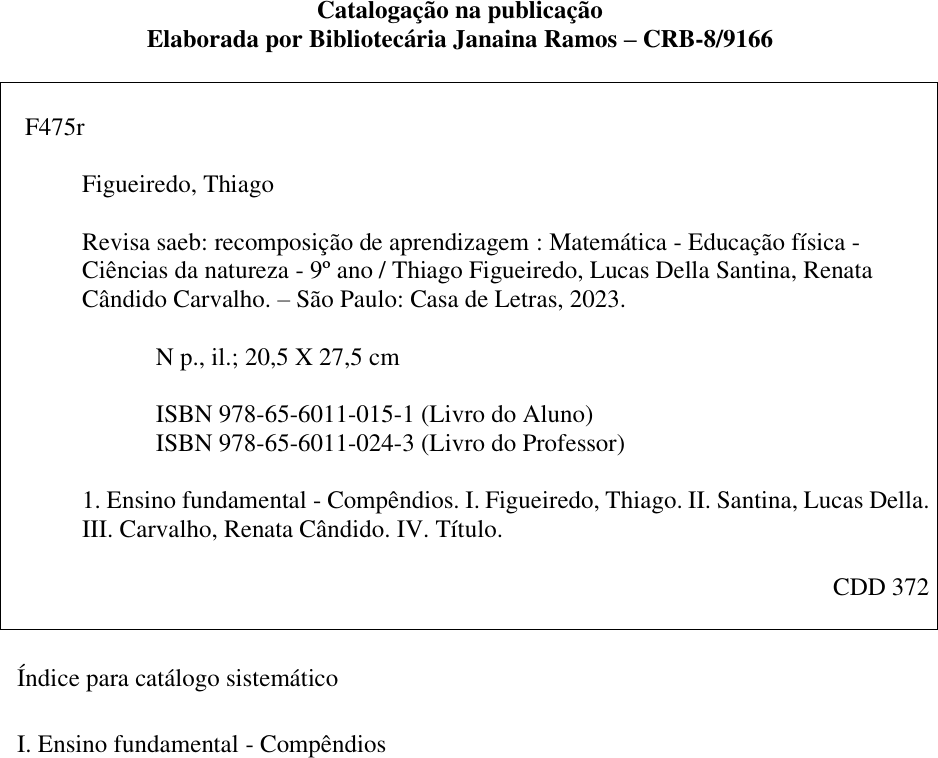
\includegraphics[width=.5\textwidth]{../fichas/9MAT.png}

\vfill

\textsc{casa de letras e gráfica ltda.}\\
Rua Fradique Coutinho, 1139, andar 2, sala 2\\
CEP 05416--011 -- São Paulo/\textsc{sp}, Brasil\\
Telefone: (11) 3914--7790\\\smallskip
www.casadeletras.com.br\\

\endgroup
\pagebreak
     % [Créditos]
% nothing			is level -3
% \book				is level -2
% \part				is level -1
% \chapter 			is level 0
% \section 			is level 1
% \subsection 		is level 2
% \subsubsection 	is level 3
% \paragraph 		is level 4
% \subparagraph 	is level 5
\setcounter{secnumdepth}{2}
\setcounter{tocdepth}{0}
 
% \renewcommand{\contentsname}{Índex} 	% Trocar nome do sumário para 'Índex'
%\ifodd\thepage\relax\else\blankpage\fi 	% Verifica se página é par e coloca página branca
%\tableofcontents*

\pagebreak
{\begingroup\mbox{}\pagestyle{empty}
\pagestyle{empty} 
% \renewcommand{\contentsname}{Índex} 	% Trocar nome do sumário para 'Índex'
%\ifodd\thepage\relax\else\blankpage\fi 	% Verifica se página é par e coloca página branca
\addtocontents{toc}{\protect\thispagestyle{empty}}
%\addtocontents{toc}{\vspace*{-.1cm}}
\tableofcontents*\clearpage\endgroup}

%!TEX root=./LIVRO.tex
\chapter{APRESENTAÇÃO}

O \textbf{SISTEMA DE AVALIAÇÃO DA EDUCAÇÃO BÁSICA (SAEB)} É UM CONJUNTO
DE AVALIAÇÕES EXTERNAS EM LARGA ESCALA QUE PERMITE AO INSTITUTO NACIONAL
DE ESTUDOS E PESQUISAS EDUCACIONAIS ANÍSIO TEIXEIRA (INEP) REALIZAR UM
DIAGNÓSTICO DA EDUCAÇÃO BÁSICA BRASILEIRA E DE FATORES QUE PODEM
INTERFERIR NO DESEMPENHO DOS ESTUDANTES.

POR MEIO DE TESTES E QUESTIONÁRIOS, APLICADOS A CADA DOIS ANOS NA REDE
PÚBLICA E EM UMA AMOSTRA DA REDE PRIVADA, O SAEB REFLETE OS NÍVEIS DE
APRENDIZAGEM DEMONSTRADOS PELOS ESTUDANTES AVALIADOS, EXPLICANDO ESSES
RESULTADOS A PARTIR DE UMA SÉRIE DE INFORMAÇÕES CONTEXTUAIS.

O SAEB PERMITE QUE AS ESCOLAS E AS REDES MUNICIPAIS E ESTADUAIS DE
ENSINO AVALIEM A QUALIDADE DA EDUCAÇÃO OFERECIDA AOS ESTUDANTES. O
RESULTADO DA AVALIAÇÃO É UM INDICATIVO DA QUALIDADE DO ENSINO BRASILEIRO
E OFERECE SUBSÍDIOS PARA ELABORAÇÃO, MONITORAMENTO E APRIMORAMENTO DE
POLÍTICAS EDUCACIONAIS, SEMPRE COM BASE EM EVIDÊNCIAS.

AS MÉDIAS DE DESEMPENHO DOS ESTUDANTES, APURADAS NO SAEB, JUNTAMENTE COM
AS TAXAS DE APROVAÇÃO, REPROVAÇÃO E ABANDONO, APURADAS NO CENSO ESCOLAR,
COMPÕEM O ÍNDICE DE DESENVOLVIMENTO DA EDUCAÇÃO BÁSICA (IDEB).

REALIZADO DESDE 1990, O SAEB PASSOU POR UMA SÉRIE DE APRIMORAMENTOS
TEÓRICO-METODOLÓGICOS AO LONGO DAS EDIÇÕES. A EDIÇÃO DE 2019 MARCA O
INÍCIO DE UM PERÍODO DE TRANSIÇÃO ENTRE AS MATRIZES DE REFERÊNCIA
UTILIZADAS DESDE 2001 E AS NOVAS MATRIZES ELABORADAS EM CONFORMIDADE COM
A BASE NACIONAL COMUM CURRICULAR (BNCC).

\section*{REVISA SAEB: REFORÇO ESCOLAR}

COMO O PRÓPRIO NOME DIZ, A EDUCAÇÃO BÁSICA É AQUELA EM QUE SE PROMOVE A
FORMAÇÃO MAIS ESSENCIAL DOS ALUNOS. O SISTEMA DE AVALIAÇÃO DA EDUCAÇÃO
BÁSICA (SAEB) AJUDA NA DETECÇÃO DOS PONTOS FORTES E FRACOS NA FORMAÇÃO
DOS ALUNOS EM ESTADOS, EM MUNICÍPIOS, EM ESCOLAS, FUNCIONANDO COMO UM
PARÂMETRO PARA QUE PROBLEMAS SEJAM SOLUCIONADOS E PARA QUE, ANO APÓS
ANO, ESSA FORMAÇÃO EVOLUA E AJUDE NO CRESCIMENTO DESSAS ESCOLAS, DESSES
MUNICÍPIOS E DESSES ESTADOS.

A PREPARAÇÃO ADEQUADA PARA AVALIAÇÕES EM LARGA ESCALA, COMO A DO SAEB, É
IMPORTANTE PARA QUE, NO MOMENTO DA PROVA, OS ALUNOS POSSAM ESTAR ATENTOS
E TRANQUILOS PARA DAREM O MELHOR POSSÍVEL DE SEU POTENCIAL. ASSIM, UM
MATERIAL DIDÁTICO DE APOIO QUE, DE FATO, PROMOVA ESSA PREPARAÇÃO É O
MAIOR DOS ALIADOS PARA PROFESSORES E GESTORES. ESTE MATERIAL TEM
EXATAMENTE ESTA INTENÇÃO: GARANTIR UM MELHOR APROVEITAMENTO DE CADA
ESTUDANTE NA RESOLUÇÃO DE ATIVIDADES, PARA QUE CONSIGAM RESULTADOS
EXCELENTES NESSA TRAJETÓRIA DE AVALIAÇÃO.

O \textbf{REVISA SAEB} ESTÁ DIVIDIDO EM 18 VOLUMES, DISTRIBUÍDOS, AO
LONGO DO ENSINO FUNDAMENTAL, DA SEGUINTE MANEIRA:

\begin{itemize}
\item
  NOS ANOS INICIAIS, PARA O \textbf{PRIMEIRO}, O \textbf{SEGUNDO}, O
  \textbf{TERCEIRO} E O \textbf{QUARTO ANO}, E NOS ANOS FINAIS, PARA O
  \textbf{SEXTO}, O \textbf{SÉTIMO} E O \textbf{OITAVO ANO}, EXISTE UM
  VOLUME POR ANO DE LÍNGUA PORTUGUESA E EXISTE UM VOLUME POR ANO DE
  MATEMÁTICA.
\item
  O \textbf{QUINTO ANO} APRESENTA UMA ESTRUTURA ESPECIAL. EM UM VOLUME,
  APARECEM ESTES COMPONENTES: LÍNGUA PORTUGUESA, ARTE E CIÊNCIAS
  HUMANAS. EM OUTRO VOLUME, APARECEM ESTES COMPONENTES: MATEMÁTICA,
  EDUCAÇÃO FÍSICA E CIÊNCIAS DA NATUREZA.
\item
  O \textbf{NONO ANO} TAMBÉM APRESENTA UMA ESTRUTURA ESPECIAL. SÃO DOIS
  VOLUMES: UM CONTÉM LÍNGUA PORTUGUESA, ARTE, LÍNGUA INGLESA E CIÊNCIAS
  HUMANAS; O OUTRO CONTÉM MATEMÁTICA, EDUCAÇÃO FÍSICA E CIÊNCIAS DA
  NATUREZA.
\end{itemize}

CADA VOLUME, EM CADA COMPONENTE, ESTÁ DIVIDIDO EM MÓDULOS TEMÁTICOS (DE
UMA OU DUAS AULAS), E CADA MÓDULO CONTA COM A ESTRUTURA DESCRITA A
SEGUIR.

\begin{itemize}
\item
  A \textbf{ABERTURA DO MÓDULO} APRESENTA UM RESUMO TEÓRICO DE
  CONTEXTUALIZAÇÃO, VINCULADO, PRINCIPALMENTE, A HABILIDADES DAS
  MATRIZES DO SAEB, MAS TAMBÉM A ALGUMAS HABILIDADES DA BNCC QUE TÊM
  RELAÇÃO COM ESSAS PRIMEIRAS HABILIDADES.
\item
  NA SEQUÊNCIA, ABRE-SE UMA SEÇÃO DE \textbf{ATIVIDADES}, QUE CONTÉM
  EXERCÍCIOS DE MODELOS VARIADOS PARA RETOMADA E FIXAÇÃO
  DO CONTEÚDO TRAZIDO PELO MÓDULO.
\item
  NO FECHAMENTO DE CADA MÓDULO, SURGE UMA SEÇÃO CHAMADA \textbf{TREINO},
  QUE CONTÉM TRÊS ITENS (QUESTÕES NO MODELO DO INEP, QUE É O MESMO
  UTILIZADO NOS TESTES COGNITIVOS DO SAEB). CADA ITEM CHECA O
  DESENVOLVIMENTO DE UMA HABILIDADE DAS MATRIZES DO SAEB E, SEMPRE QUE
  HÁ CONEXÃO, ESTÁ VINCULADO A UMA HABILIDADE DA BNCC DO ANO
  CORRESPONDENTE.
\item
  OS VOLUMES SE ENCERRAM COM QUATRO \textbf{SIMULADOS}, PARA SEREM
  APLICADOS BIMESTRALMENTE. AO LONGO DOS QUATROS SIMULADOS, TODAS AS
  HABILIDADES DAS MATRIZES DO SAEB, EM CADA ANO, SÃO TRABALHADAS, DESDE
  QUE VINCULADAS A CONTEÚDOS PREVISTOS PELA BNCC PARA O ANO EM
  ESPECÍFICO. IGUALMENTE COMPOSTOS DE ITENS, EM NÚMEROS VARIADOS, OS
  SIMULADOS TAMBÉM APRESENTAM, SEMPRE QUE HÁ CONEXÃO, HABILIDADES DA
  BNCC.
\end{itemize}

%\addcontentsline{toc}{chapter}{...}

%\chapter{1. Números e mais números}

\coment{Habilidades da BNCC: EF05MA01, EF05MA10, EF05MA11.}

\colorsec{Habilidades do SAEB}

\begin{itemize}
\item Escrever números racionais (naturais de até 6 ordens, representação
fracionária ou decimal finita até a ordem dos milésimos) em sua
representação por algarismos ou em língua materna ou associar o registro
numérico ao registro em língua materna.

\item Identificar a ordem ocupada por um algarismo ou seu valor posicional
(ou valor relativo) em um número natural de até 6 ordens.

\item Comparar ou ordenar números racionais (naturais de até 6 ordens,
representação fracionária ou decimal finita até a ordem dos milésimos),
com ou sem suporte da reta numérica.

\item Compor ou decompor números naturais de até 6 ordens na forma aditiva,
ou em suas ordens, ou em adições e multiplicações.

\item Comparar diferentes sentenças de adições ou de subtrações de dois números naturais.

\item Determinar o número desconhecido que torna verdadeira uma igualdade
que envolve as operações fundamentais com números naturais de até 6
ordens.
\end{itemize}

\conteudo{Professor, neste módulo devemos revisar os conceitos de montagem de
números, frisando muito as classes e até a 6º ordem. É muito importante
os alunos finalizarem o módulo sabendo o valor posicional e relativo de
cada algarismo quando estão em determinada ordem.

Além disso, deve-se trabalhar minuciosamente a decomposição dos números e sua
escrita por extenso.

%Produzir uma tabela igual à apresentada como modelo.

Valor posicional ou relativo: é o valor que o algarismo assume dependendo da classe e da ordem em que ele está posicionado no número.

%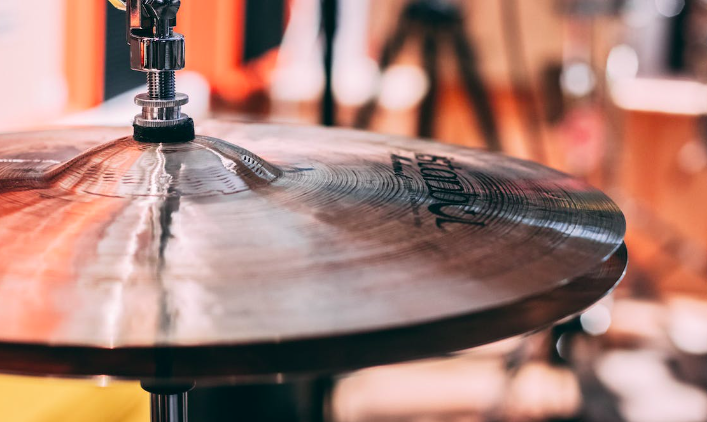
\includegraphics[width=3.55128in,height=1.66618in]{media/image1.png}

Exemplo: No número 352.146, o algarismo 5 possui valor posicional ou
relativo igual a 50.000, pois ocupa a 5º ordem, a qual está dentro da
classe dos milhares, ou seja, está na posição da dezena de milhar; sendo
assim, 5 x 10.000 = 50.000.}

\colorsec{Atividades}

\num{1} Escreva dentro dos retângulos o valor posicional dos algarismos
destacados, ou seja, o valor que eles assumem de acordo com a posição que ocupam no número.

%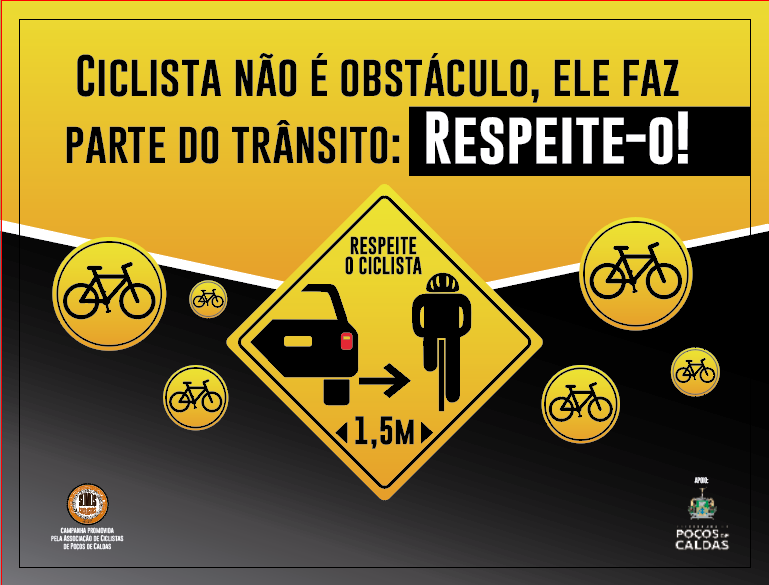
\includegraphics[width=3.65385in,height=2.00568in]{media/image2.png}

%Fazer uma figura conforme a indicada acima trocando os números da seguinte forma:
%
%OBS: os retângulos devem ser maiores (dobro de tamanho do indicado) pois
%assim o aluno consegue escrever por extenso o número dentro dele.


%824.345 e o 8 deve ser o número em destaque associado ao box

%375.678 e os números 7 devem estar associados a cada um dos retângulos
  %além de estarem em destaque.

%148.521 e os números 1 devem estar associados a cada um dos retângulos além de estarem em destaque.

%795.654 todos os números devem estar associados a um box e o número inteiro deve estar em destaque. Deveremos ter então 6 boxes e cada um deve estar associado a um dos algarismos do número.


\coment{
a) O algarismo 8 destacado tem valor posicional igual a 800.000 (oitocentos mil), já que se encontra na centena de milhar.
b)  O primeiro algarismo 7 destacado tem valor posicional igual a 70.000 (setenta mil), já que se encontra na dezena de milhar.
Já o segundo algarismo 7 destacado tem valor posicional igual a 70 (setenta), já que está posicionado na dezena comum.
c)  O primeiro algarismo 1 destacado tem valor posicional igual a 100.000
  (cem mil), já que se encontra na centena de milhar.
Já o segundo algarismo 1 destacado tem o valor posicional igual a 1 (uma
unidade), já que se encontra na unidade comum.
d) O algarismo 7 destacado tem valor posicional igual a 700.000
  (setecentos mil), já que está na centena de milhar.
O algarismo 9 destacado tem valor posicional igual a 90.000 (noventa
mil), já que está na dezena de milhar.
O primeiro algarismo 5 destacado tem valor posicional igual a 5.000
(cinco mil), já que está na unidade de milhar.
O algarismo 6 destacado tem valor posicional igual a 600 (seiscentos), já
que está na centena comum.
O segundo algarismo 5 destacado tem valor posicional igual a 50
(cinquenta), já que está na dezena comum.
O algarismo 4 destacado tem valor posicional igual a 4 (4 unidades), já
que está na unidade comum.}

\num{2} Decomponha os números a seguir de acordo com o valor posicional de
cada algarismo.

\begin{escolha}
\item 32.084

\linhas{1}

\item 26.587

\linhas{1}

\item 2.105

\linhas{1}
\end{escolha}

\coment{
a) 30.000 + 2.000 + 80 + 4 ou
3 x 10.000 + 2 x 1.000 + 0 x 100 + 8 x 10 + 4. 
Além disso, utilize o exercício para treinar a escrita dos alunos. Exemplo: trinta e dois mil e
oitenta e quatro.
b) 20.000 + 6.000 + 500 + 80 + 7 ou 2 x 10.000 + 6 x 1.000 + 5 x 100 + 8 x 10 + 7.
c)  2.000 + 100 + 5 ou 2 x 1.000 + 1 x 100 + 0 x 10 + 5.}

\num{3} Monte os números compostos e registre-os nos locais correspondentes.

\begin{escolha}
\item 7 unidades de milhar, 5 centenas e 4 unidades: \preencher

\item 3 dezenas de milhar, 7 dezenas e 2 unidades: \preencher

\item 9 centenas de milhar, 5 unidades de milhar e 6 centenas: \preencher

\item 2 unidades de milhar, 6 centenas e 3 unidades: \preencher
\end{escolha}

\coment{
a)  7.504.
b)  30.072.
c)  905.600.
d)  2.603.

Professor, devemos explorar bem a escrita dos números a partir da decomposição, pois muitos alunos desenvolvem
dificuldades, conseguindo fazer a decomposição, mas sem compreender a volta (montagem dos números decompostos).}

\num{4} Ligue os retângulos da coluna com 1 a um corresponde da coluna 2
que represente a escrita por extenso do número indicado na primeira
coluna.

\begin{multicols}{2}

\red{352.700}

\red{200.015}

\red{20.003}

\red{314.000}

\blue{Trezentos e catorze mil}

\blue{Vinte mil e três}

\blue{Trezentos e cinquenta e dois mil e setecentos}

\blue{Duzentos mil e quinze}
\end{multicols}

\coment{
352.700 deve estar ligado a "trezentos e cinquenta e dois mil e setecentos".
200.015 deve estar ligado a "duzentos mil e quinze".
20.003 deve estar ligado a "vinte mil e três".
314.000 deve estar ligado a "trezentos e catorze mil".}

\num{5} Utilizando o material dourado, Ana Letícia montou o seguinte número:

%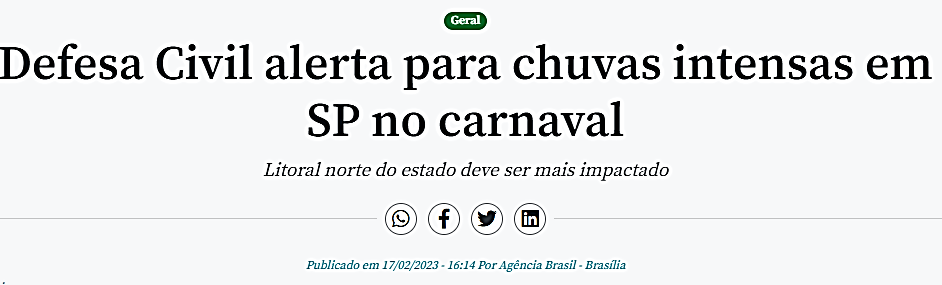
\includegraphics[width=5.02820in,height=0.67949in]{media/image4.png}

%Construir uma figura dessa forma mantendo a quantidade de 1 cubo grande (10 cubinhos x 10 cubinhos x 10 cubinhos), 5 placas (10 cubinhos x10 cubinhos) e 9 cubinhos pequenos.

Qual o número representado por Ana Letícia?

\coment{ 1.509
1 x 1.000 + 5 x 100 + 1 x 9 = 1.509.}

\num{6} Leia o diálogo que ocorreu entre um vendedor de carros e a pessoa interessada em comprar o carro.

%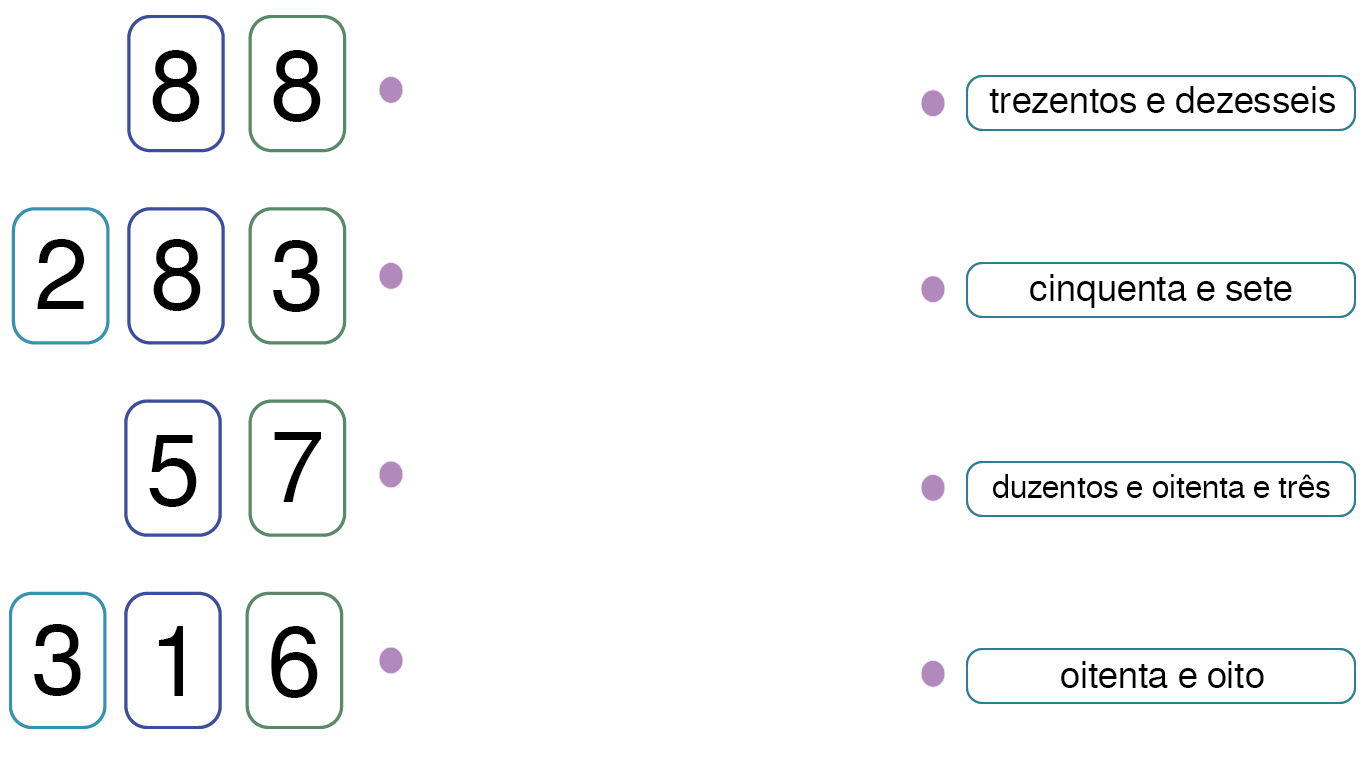
\includegraphics[width=3.09167in,height=2.07953in]{media/image5.png}
%https://img.freepik.com/fotos-gratis/mulher-independente-financeira-comprando-carro-novo_232149571908.jpg?w=1060\&t=st=1677433708~exp=1677434308~hmac=4c085c446d424d16dad6fc6c14af3bf2c68c78d300da5897efac341ef60d6deb

%Fazer um balão de diálogo saindo do vendedor com os seguintes escritos: "Este modelo, com todos os equipamentos, está sendo vendido por noventa e três mil novecentos e noventa reais".

Escreva com algarismos, em reais, o valor pelo qual o vendedor pretende vender o carro ao interessado.

\linhas{1}

\coment{93.990 reais ou R$93.990,00. 

Professor, explore outros exemplos com os alunos
para que realmente entendam como escrever os números utilizando algarismos.}

\num{7} Realize a correspondência entre os retângulos da coluna 1 e os
círculos da segunda coluna, traçando linhas retas.

\begin{multicols}{2}
\blue{O maior número com exatamente 4 ordens.}

\blue{O segundo maior número formado por 4 ordens.}

\blue{Um número ímpar com 6 ordens.}

\blue{Um número de 6 ordens com algarismo da unidade de milhar igual a 3}

\red{143.254}

\red{644.821}

\red{9.999}

\red{9.998}
\end{multicols}

\coment{
"O maior número com exatamente 4 ordens" deverá estar ligado a 9.999.
"O segundo maior número formado por 4 ordens" deverá estar ligado a 9.998.
"Um número ímpar com 6 ordens" deverá estar ligado a 644.821.
"Um número de 6 ordens com algarismo da unidade de milhar igual a 3" deverá estar ligado a 143.254.

Professor, explore ao máximo o conceito de par e ímpar e já comece a
introduzir o conceito sequencial dos números naturais, em que após um par
sempre vem um ímpar e em que depois de um ímpar sempre vem um par (desde que
estejam todos os números naturais escritos).

Além disso, já pode ser introduzido o conceito de sucessor e antecessor, que aparecerá mais à frente, dizendo que 9.999 é sucessor de 9.998, e que 9.998
é o antecessor de 9.999.}

\num{8} Felipe quer realizar uma corrida e resolveu planejá-la. Para isso,
fez uma linha reta e nela marcou intervalos de 1 km, como na representação a seguir.

%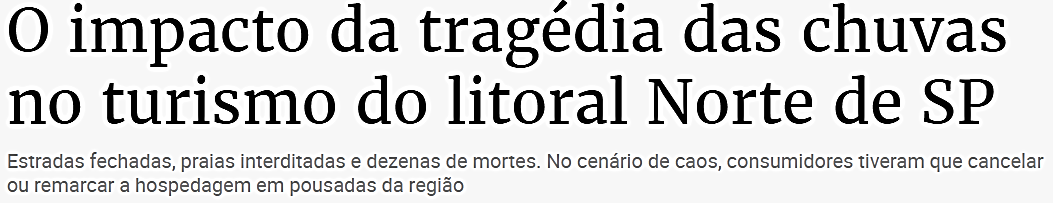
\includegraphics[width=5.90556in,height=0.79514in]{media/image6.png}

%Colocar B no lugar do X no desenho pedido.

%Colocar um desenho de uma pista de corrida com as marcações da forma que estão apresentadas acima. A ponto a deve estar no km 0 e o número de marcações até o ponto B não podem ser alteradas.

Ele pretende começar no ponto A e terminar no ponto B. Se Felipe
conseguir completar a corrida, ele terá parado na marcação:

\begin{escolha}
\item
  Km 9
\item
  Km 10
\item
  Km 11
\item
  Km 12
\end{escolha}

\coment{
Como ele saiu do ponto A, que está em cima da marcação km 0, e chegou ao
ponto B, que está a 12 marcações de distância do ponto, podemos concluir
que ele parou no km 12, ou seja, percorreu 12 km.

Explore ao máximo com os alunos a colocação dos números na reta numérica,
já que é um conceito essencial para outros tópicos do conteúdo.}

\num{9} Complete a frase com o número que representa quanto mede cada um
dos objetos indicados a seguir.

\begin{escolha}
\item O lápis a seguir mede \preencher\coment{11 cm}

%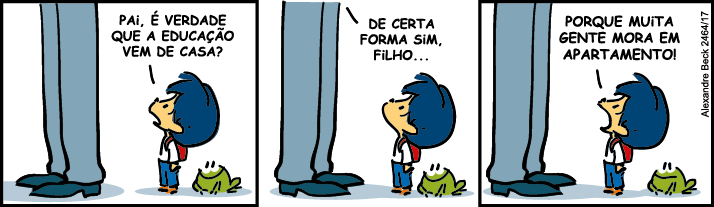
\includegraphics[width=4.00868in,height=0.70839in]{media/image7.png}
%Construir a imagem acima. O lápis na régua deve sair exatamente do 0 e chegar exatamente no 11. Deixar um pedaço de linha nos locais indicados por traços nos itens acima.

\item A borracha representada mede \preencher\coment{5 cm}

%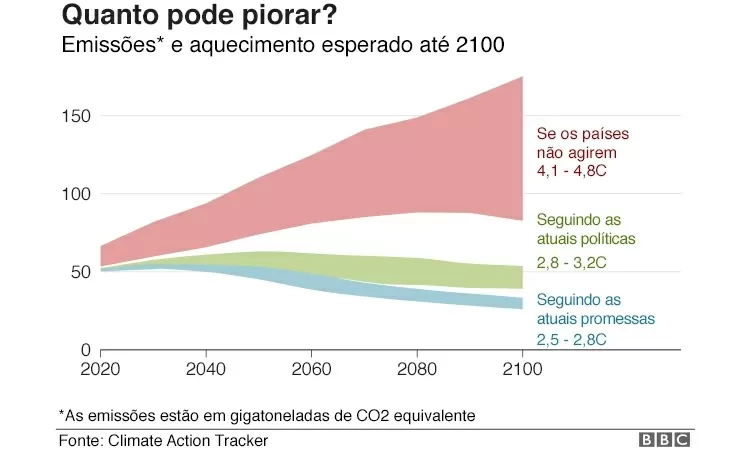
\includegraphics[width=3.24167in,height=0.84476in]{media/image8.png}
%Construir a imagem acima. A borracha deve sair exatamente do zero e chegar exatamente no 5. Deixar um pedaço de linha nos locais indicados por traços nos itens acima.

\item O apontador da imagem mede \preencher\coment{3 cm}

%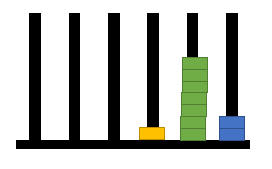
\includegraphics[width=3.19167in,height=0.78934in]{media/image9.png}

%Construir uma imagem semelhante à de cima. O apontador deve começar exatamente no 3 e terminar exatamente no 6. Deixar um pedaço de linha nos locais indicados por traços nos itens acima.

\item A tesoura a seguir mede \preencher\coment{10 cm}

%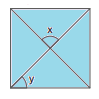
\includegraphics[width=2.65717in,height=1.37500in]{media/image10.png}

%Construir uma imagem semelhante à de cima. Deixar um pedaço de linha nos locais indicados por traços nos itens acima.

%A tesoura deve sair exatamente do 1 e chegar exatamente no 11
\end{escolha}

\coment{Professor, explore bastante a habilidade de medir com o auxílio da reta
numérica, principalmente quando o início não está no zero. Esse conceito é
muito útil para entendimento de assuntos que virão em outros anos e
trabalhar bastante agora pode ser extremamente importante para o desenvolvimento do aluno em anos
posteriores.}

\num{10} A esferas representadas a seguir fazem parte de um jogo conhecido como
"bilhar" ou "sinuca".

%
\includegraphics[width=1.40833in,height=1.33406in]{media/image11.png}
%https://img.freepik.com/vetores-premium/%bola-de-bilhar-azul-com-numero-2-snooker-ou-bola-de-loteria-em-fundo-branco-ilustracao_390775-925.jpg?w=740
%
%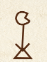
\includegraphics[width=1.66667in,height=1.61877in]{media/image12.png}
%
%https://img.freepik.com/vetores-premium/bilhar_672017-1383.jpg?w=740
%
%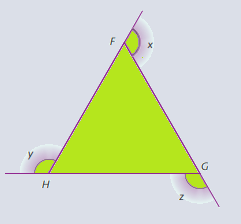
\includegraphics[width=1.68333in,height=1.36449in]{media/image13.png}
%
%https://img.freepik.com/psd-premium/ilustracao-3d-da-bola-de-bilhar-oito_446709-517.jpg?w=740
%
%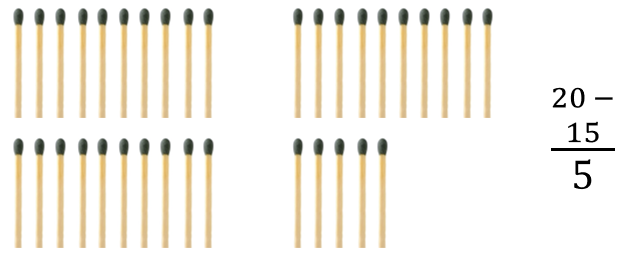
\includegraphics[width=1.61667in,height=1.60236in]{media/image14.png}
%
%https://img.freepik.com/psd-premium/bola-de-bilhar-3d-numero-9_592419-130.jpg?w=740
%
%Colocar as bolinhas na mesma linha

Observando os números representados em cada esfera, responda:

\begin{escolha}
\item  Qual o maior número?

\linhas{1}
\item  Qual o menor número, com exatamente 3 ordens, que se pode formar?

\linhas{1}
\item  Qual o maior número par que se pode formar?

\linhas{1}
\end{escolha}

\coment{
a)  9 (nove).
b)  278 (duzentos e setenta e oito).
c)  9.872 (nove mil oitocentos e setenta e dois).
Explore mais exemplos com os alunos para estimular a formação de números e a criatividade de cada um deles.}

\section{Treino}


\num{1} Amanda estava brincando no escritório de seu pai quando encontrou um pedaço de papel.

%
\includegraphics[width=3.30833in,height=2.17391in]{media/image15.png}
%https://img.freepik.com/vetores-gratis/vetor-de-fundo-de-design-de-pedaco-de-papel-rasgado_1055-13108.jpg?w=900\&t=st=1677434705~exp=1677435305~hmac=787f679840c02b57af4cb87ef851030bb83880366602641e4486462d6d3553f8
%No pedaço de papel colocar bem grande a frase abaixo escrita:

Faturamento semestral: 650.734 reais

Lembrando das aulas de matemática, ela resolveu decompor o número escrito
no papel. Qual a decomposição correta que Amanda deverá fazer desse
número?

\begin{escolha}
\item
  600.000 + 50.000 + 700 + 30 + 4
\item
  600.000 + 5.000 + 70 + 3 + 4
\item
  600.000 + 500 + 700 + 30 + 4
\item
  60.000 + 50.000 + 70 + 300 + 4
\end{escolha}

\coment{SAEB: - Compor ou decompor números naturais de até 6 ordens na forma aditiva, ou em suas ordens, ou em adições e multiplicações.
BNCC: EF05MA01 - Ler, escrever e ordenar números naturais até a ordem das centenas de milhar com
compreensão das principais características do sistema de numeração decimal.

a) Correta. 600 000 + 50 000 + 700 + 30 + 4.
b) Incorreta. Não se trata de 5.000, mas de 50.000; não se trata de 70, mas de 700; não se trata de 3, mas de 30.
c) Incorreta. Não se trata de 500, mas de 50.000.
d) Incorreta. Não se trata de 60.000, nem de 70, nem de 300.}

\num{2} Na reta numérica a seguir, o ponto P representa o número 540 e o
ponto U representa o número 590.

%
\includegraphics[width=3.03205in,height=0.81228in]{media/image16.png}
%Na figura acima ao invés de 960 favor colocar 540 e no lugar de 1 010 colocar 590.

Em qual ponto temos a representação do número 570, sabendo-se que a
distância entre dois pontos consecutivos é de 10 unidades?

\begin{escolha}
\item
  Q
\item
  R
\item
  S
\item
  T
\end{escolha}

\coment{SAEB: - Identificar a ordem ocupada por um algarismo ou seu valor posicional (ou valor relativo) em um número natural de até 6 ordens.
BNCC: EF05MA10 - Concluir, por meio de investigações, que a relação de igualdade existente
entre dois membros permanece ao adicionar, subtrair, multiplicar ou dividir cada um desses
membros por um mesmo número, para construir a noção de equivalência.


a) Incorreta. 570 não pode estar no ponto Q, onde estaria o número 550.
b) Incorreta. No ponto R estaria o número 560, 20 unidades além de 540.
c) Correta. O 570 estará no ponto S, pois, como no ponto P está o 540 e cada
repartição é de 10 unidades, ele deve estar no terceiro ponto após o P
sem contar o ponto S.
d) Incorreta. No ponto T estaria o número 580, 30 unidades além de 540.}

\num{3}José resolveu comprar uma linda placa com o número de sua casa.

%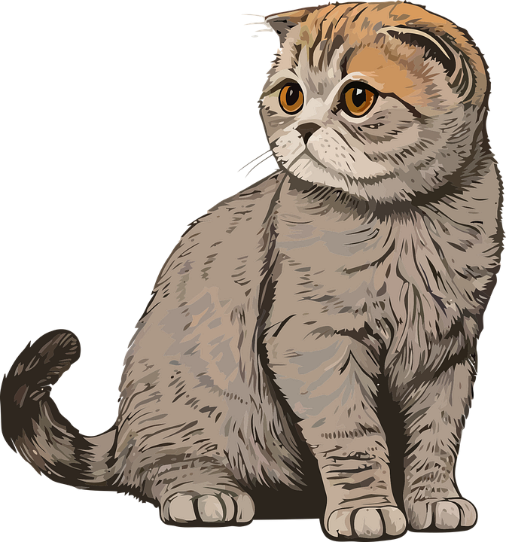
\includegraphics[width=3.02500in,height=1.48973in]{media/image17.png}
%https://img.freepik.com/fotos-gratis/numero-125_1122-1156.jpg?w=1060\&t=st=1677434865~exp=1677435465~hmac=526ac25f92ac28e692177f84842345ca95b5e246e04ca35259750459c4f3e954

Porém, na hora de efetuar a compra, não percebeu que o número estava
errado, já que o primeiro e o último algarismos estão nas posições
trocadas. Qual é o valor relativo do último algarismo no lugar em que ele se
encontra na placa errada e qual deveria ser seu valor relativo no número
correto da casa de José?

\begin{escolha}
\item
  Como está: 5.
  Como deveria ser: 50.
\item
  Como está: 50.
  Como deveria ser: 500.
\item
  Como está: 5.
  Como deveria ser: 500.
\item
  Como está: 50.
  Como deveria ser: 5.
\end{escolha}

\coment{SAEB: - Compor ou decompor números naturais de até 6 ordens na forma aditiva, ou em suas ordens, ou em adições e multiplicações.
BNCC: EF05MA10 - Concluir, por meio de investigações, que a relação de igualdade existente
entre dois membros permanece ao adicionar, subtrair, multiplicar ou dividir cada um desses
membros por um mesmo número, para construir a noção de equivalência.


a) Incorreta. Na posição correta seria a representação de 500, não de 50.
b) Incorreta. No número errado da casa de José, o 5 está na casa das unidades.
c) Correta. Como o número apresentado no enunciado está com o primeiro e o último
algarismos trocados, conclui-se que o número correto seria 521. Na placa,
o último algarismo é o 5 e tem valor relativo de 5 unidades, mas no
número correto ele estaria na centena comum, apresentando, então, um valor
relativo de 500 (quinhentos), ou cinco centenas.
d) Incorreta. No número errado se trata de 5 e, no número correto, de 500.}


\chapter{2. Multiplicar e dividir}

\colorsec{Habilidades do SAEB}

\begin{itemize}
\item Calcular o resultado de adições ou subtrações envolvendo números
naturais de até 6 ordens.

\item Calcular o resultado de multiplicações ou divisões envolvendo números
naturais de até 6 ordens.

\item Associar o quociente de uma divisão com resto zero de um número
natural de até 6 ordens por 2, 3, 4, 5 e 10 às ideias de metade, terça,
quarta, quinta e décima parte.

\item Resolver problemas de adição ou de subtração, envolvendo números
naturais de até 6 ordens, com os significados de juntar, acrescentar,
separar, retirar, comparar ou completar.

\item Resolver problemas de multiplicação ou de divisão, envolvendo números
naturais de até 6ordens, com os significados de formação de grupos
iguais (incluindo repartição equitativa e medida), proporcionalidade ou
disposição retangular.
\end{itemize}

\conteudo{Professor, talvez este seja um dos módulos mais importantes, por se
tratar das quatro operações básicas. Relembre com os alunos cada detalhe delas, bem como os
algoritmos de adição, subtração, multiplicação e divisão, dando ênfase na divisão, que geralmente é o maior desafio enfrentado
pelos alunos.

Adição:

%Fazer a imagem abaixo segundo os padrões do projeto.
%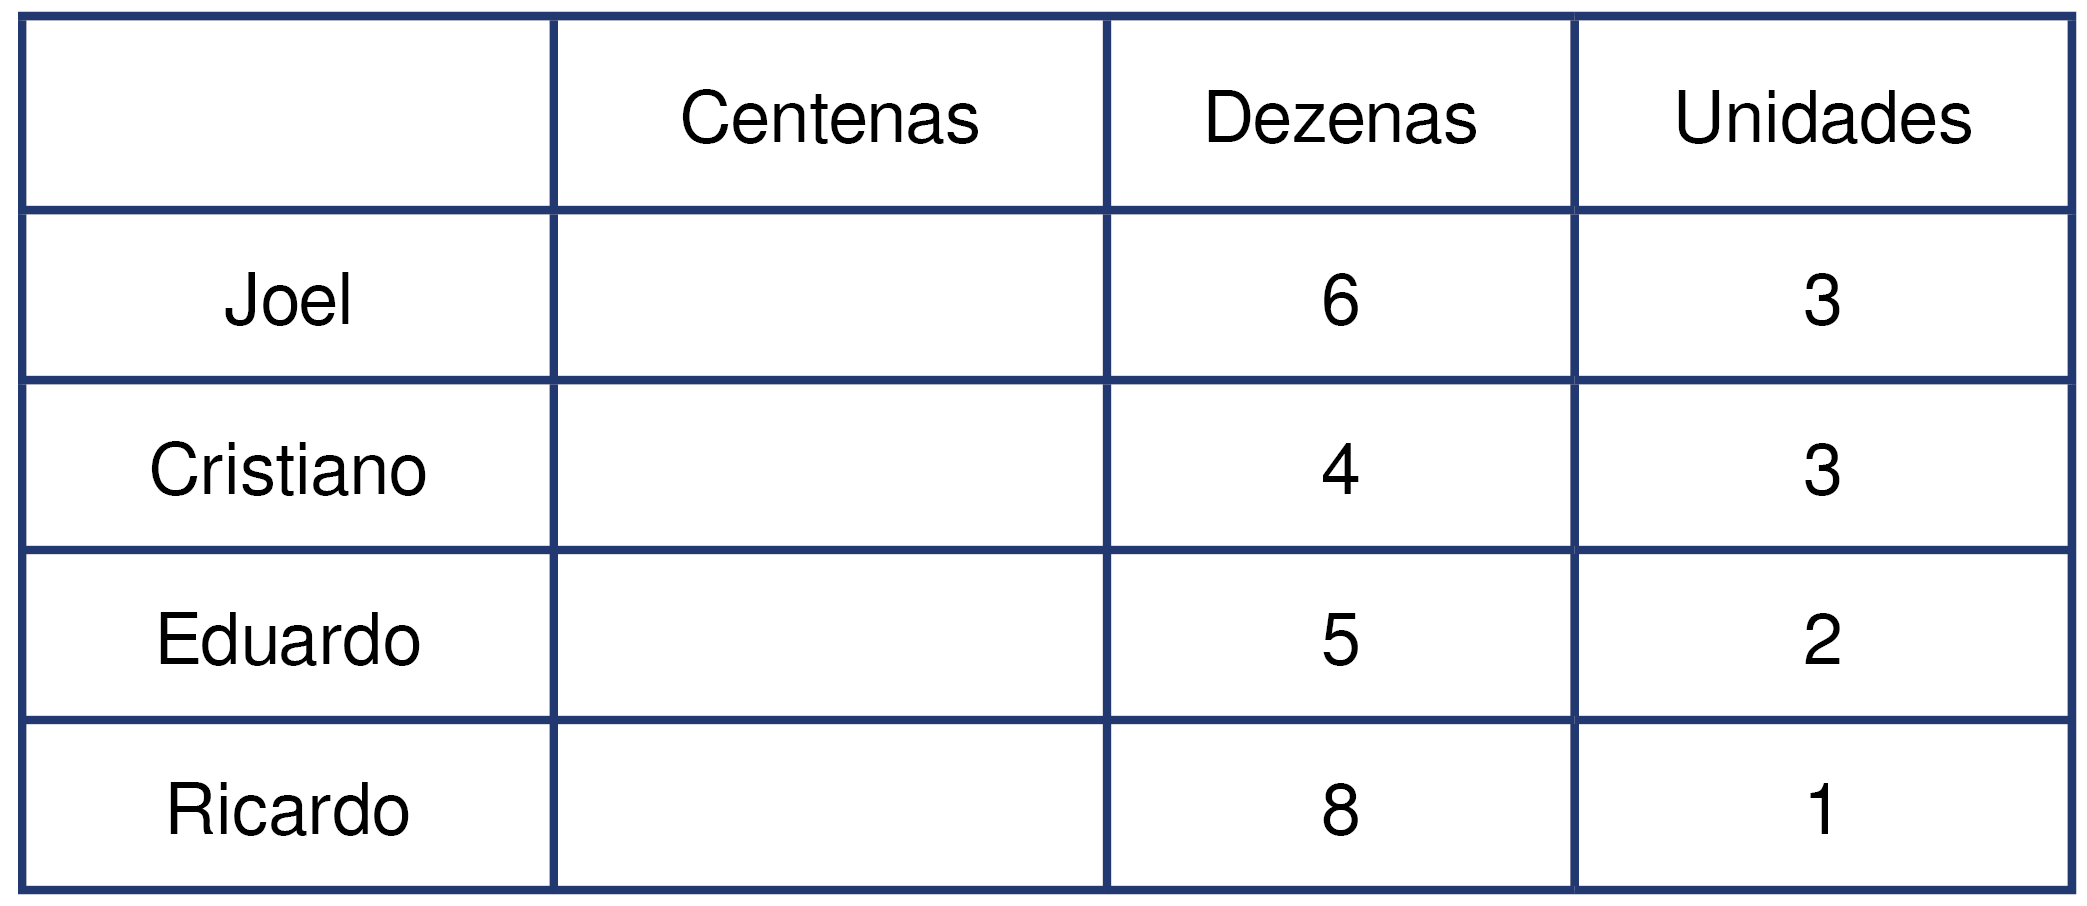
\includegraphics[width=2.26282in,height=1.19473in]{media/image18.png}

Subtração:

%Fazer a imagem abaixo segundo os padrões do projeto.
%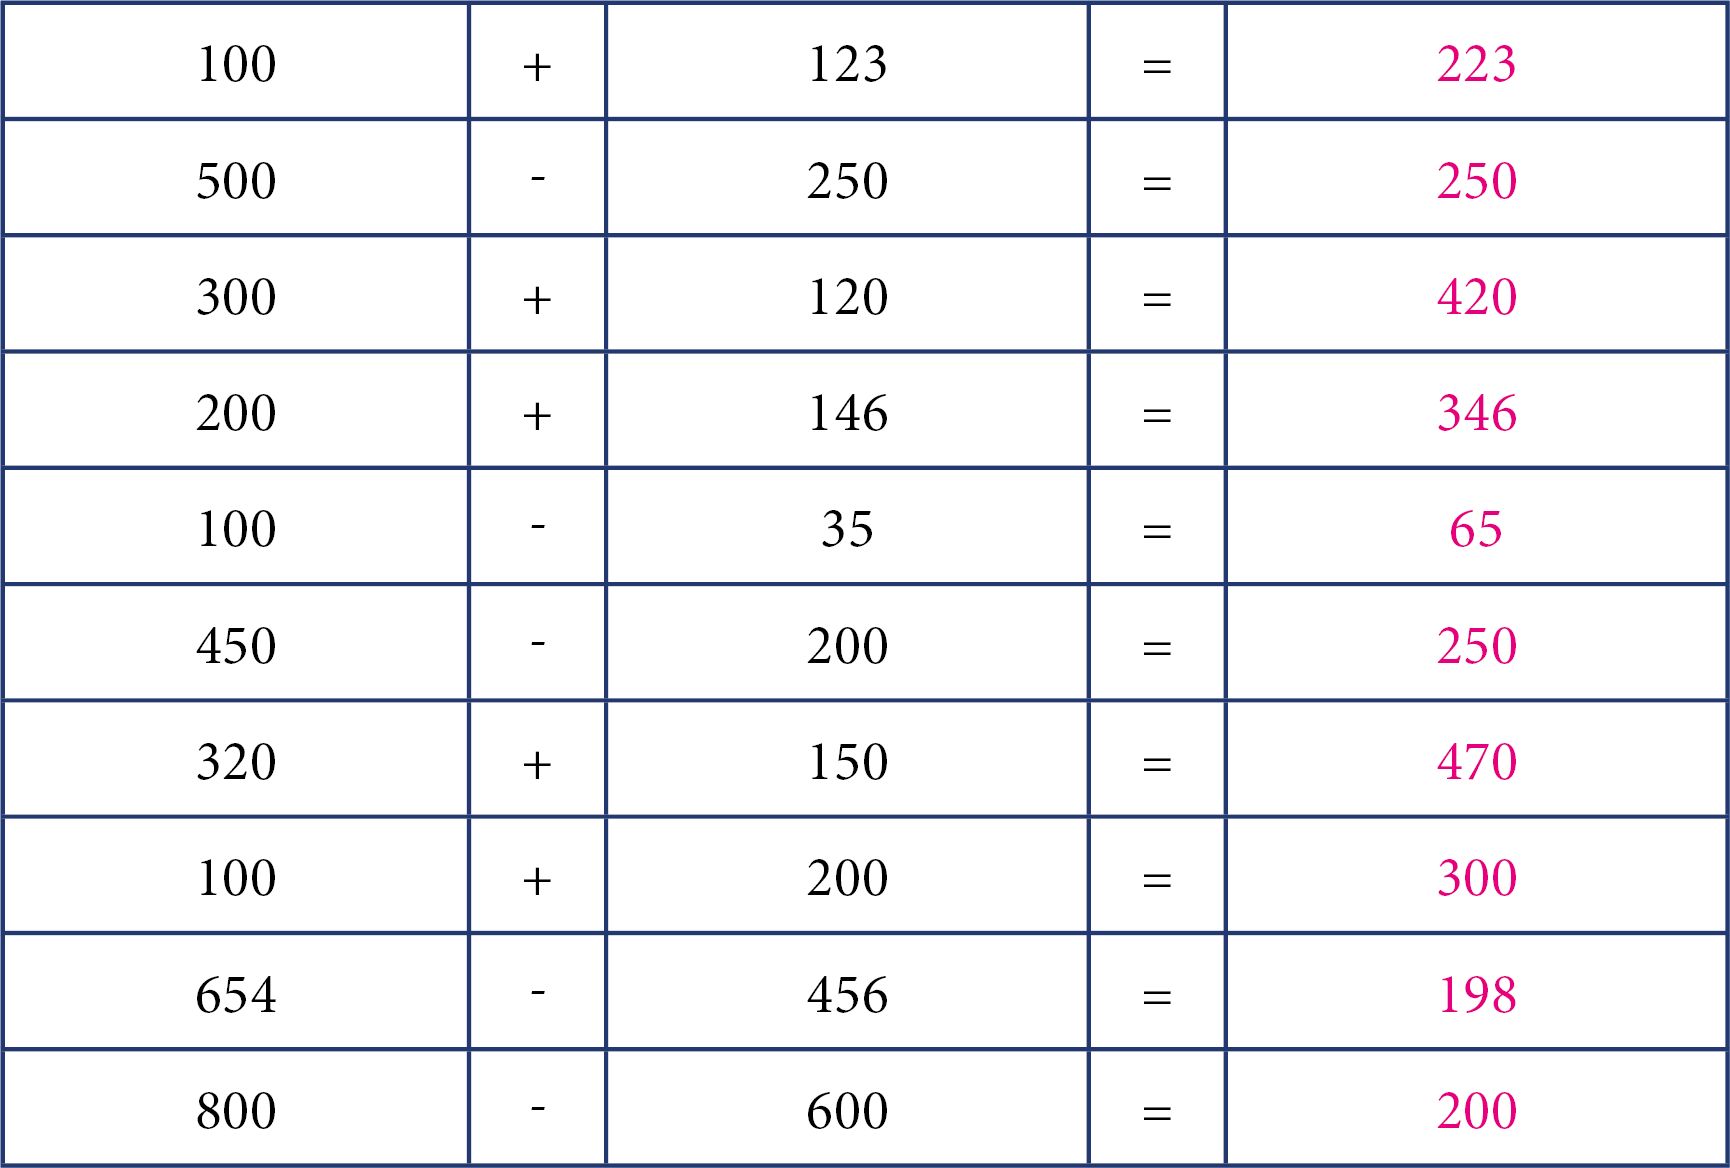
\includegraphics[width=2.55128in,height=1.04961in]{media/image19.png}

Multiplicação:

%Fazer a imagem abaixo segundo os padrões do projeto.
%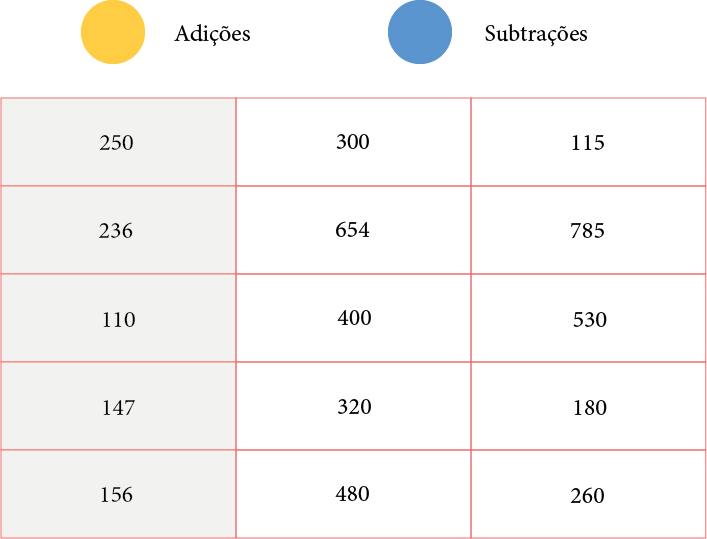
\includegraphics[width=1.92308in,height=1.09649in]{media/image20.png}

Divisão:

%Fazer a imagem abaixo segundo os padrões do projeto.
%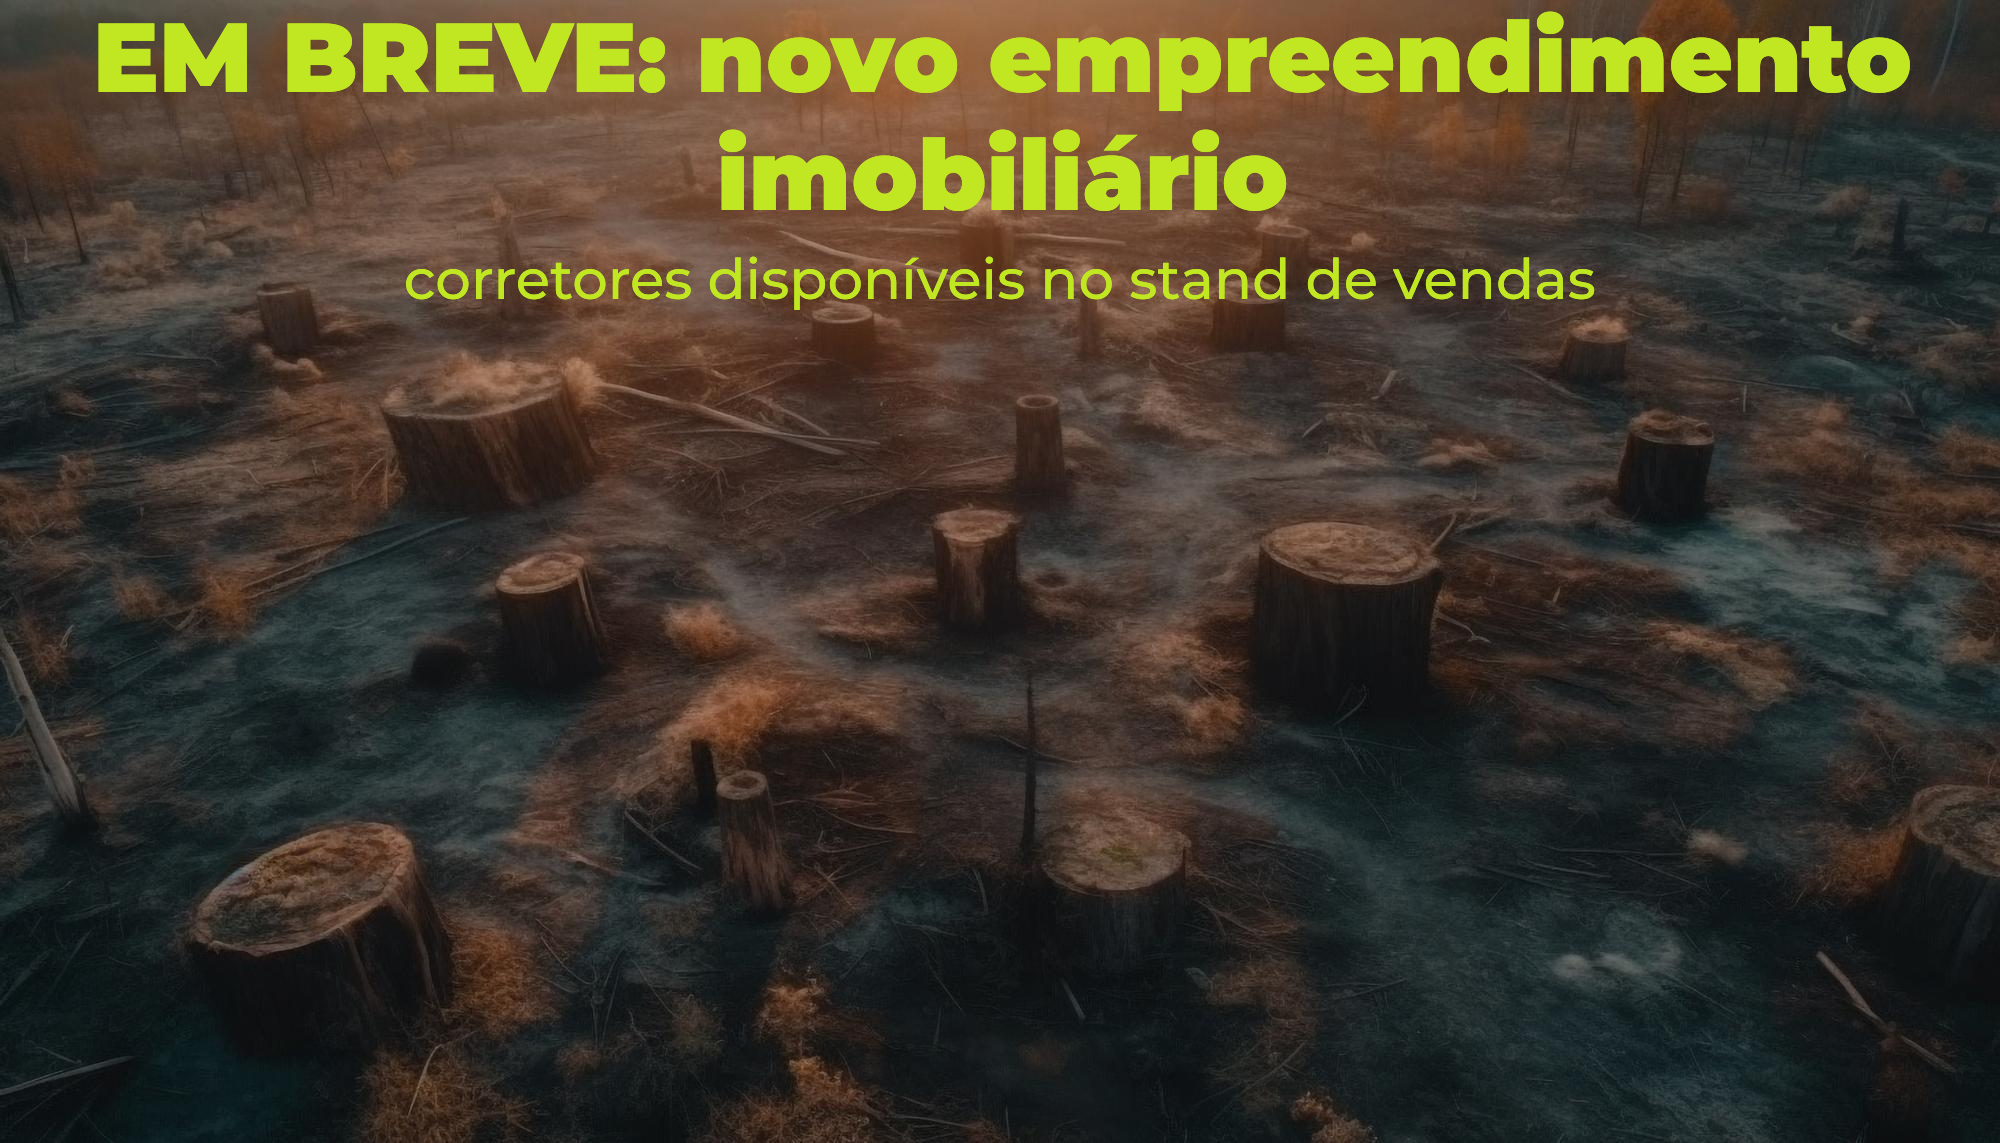
\includegraphics[width=2.26923in,height=1.66995in]{media/image21.png}
}

\colorsec{Atividades}

\num{1} Ligue cada operação que está na coluna 1 com o seu resultado correto na coluna 2.

\begin{multicols}{2}
584 -- 249 

960 -- 723 

767 -- 158 

50 -- 2 x (5 + 15) + 2 x 3 -- 2 x 2) + 3 x (10 -- 4 x 2) 

2 + 8 x 2 -- 2(1 + 2 x 3) 

50 -- {[}24 + 3 x (2 + 3 x 2{]} 

2 x 3 -- {[}10 -- 2 x (1 + 1 x 3){]} 

\columnbreak


237

609

335

4

6

18

2
\end{multicols}

\matlinhas{10}

\coment{
Professor, explore ao máximo com os alunos o conceito de quais operações
devem ser realizadas primeiro para, assim, fixar o conceito da ordem das operações.

584 -- 249 = 335

960 -- 723 = 237

767 -- 158 = 609

50 -- 2 x (5 + 15) + 2 x (3 -- 2 x 1) + 3 x (10 -- 4 x 2) = 50 -- 40 + 2
+ 6 = 18

2 + 8 x 2 -- 2(1 + 2 x 3) = 2 + 16 -- 14 = 4

50 -- {[}24 + 3 x (2 + 3 x 2{]} = 50 -- 48 = 2

2 x 4 -- {[}10 -- 2 x (1 + 1 x 3){]} = 8 -- 2 = 6}

%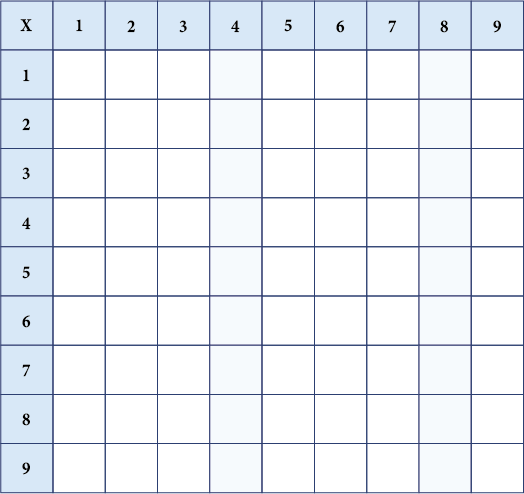
\includegraphics[width=3.00000in,height=2.02528in]{media/image22.png}

\num{2} A receita de um bolo diz que inicialmente devemos colocar 260 g de
farinha de trigo e misturar com outros ingredientes como ovos, açúcar e
leite. Um seguida, devemos colocar mais 135 g de farinha de trigo para a
massa ficar no ponto ideal. Qual foi a quantidade total de farinha
utilizada nessa receita?

%https://img.freepik.com/fotos-premium/chef-cozinheiro-confeiteiro-ou-padeiro-em-t-shirt-branca-toque-chefs-chapeu-cozinhando-na-mesa-isolada-em-fundo-rosa-pastel-em-estudio-aplicacao-de-creme-processo-de-confeccao-de-bolos-mock-up-conceito-de-comida-de-espaco-de-copia_365776-27137.jpg?w=1060

\matlinhas{3}

\coment{260 + 135 = 395 g.}

\num{3} O estado de São Paulo tem muitas cidades, sendo que muitas delas com
centenas de milhares de habitantes. A tabela mostra a população estimada
de algumas cidades paulistas.

\begin{longtable}[]{@{}ll@{}}
\toprule
Município & População estimada\tabularnewline
\midrule
\endhead
São Paulo & 12.396.372\tabularnewline
Campinas & 1.223.237\tabularnewline
Ribeirão Preto & 720.116\tabularnewline
Franca & 358.539\tabularnewline
São Carlos & 256.915\tabularnewline
\bottomrule
\end{longtable}

\fonte{Dados IBGE.}

Sem considerar a cidade de São Paulo, a soma da população estimada das
outras quatro cidades é maior ou menor do que a quantidade de habitantes
da cidade de São Paulo? Justifique com cálculos.

\matlinhas{5}

\coment{1.223.237 + 720.116 + 358.539 + 256.915 = 2.558.807.

Portanto, a soma das populações estimadas dos municípios apresentados na
tabela, exceto São Paulo, é menor que a população da cidade de São Paulo.}

\num{4} Raquel sempre gostou muito de cozinhar e,
querendo muito trabalhar com isso, ela decidiu começar uma pequena
empresa que faz doces para festas. Para o próximo final de semana, recebeu a seguinte encomenda por mensagem de texto em seu celular:

%Colocar os dados abaixo em um celular e na tela a seguinte mensagem de texto

Encomenda para a festa da Maria:

275 brigadeiros

165 beijinhos

245 cajuzinhos

Calcule o total de unidades de doces que Raquel terá que fazer para entregar essa encomenda completa.

\matlinhas{4}

\coment{275 + 165 + 245 = 685 unidades de doces.}

\num{5} Veja a pilha de caixas que Juliano guarda na garagem de sua casa.

%
\includegraphics[width=1.25000in,height=1.75995in]{media/image23.png}
%Construir uma imagem semelhante a de cima contendo três caixas e as respectivas alturas indicadas

\begin{escolha}
\item
  Qual a altura da pilha de caixas?

\matlinhas{3}

\coment{81 + 108 + 99 = 288 cm = 2,88 m}

\item
  Se Juliano inverter a ordem das caixas na hora de empilhar a altura
  total será alterada? \preencher \coment{Não}
\end{escolha}

\coment{Explorar com os alunos as propriedades das operações, principalmente a
comutativa e a associativa. Deixar que os alunos troquem a ordem das caixas
no item b para perceberem que nada será alterado na soma.}

\num{6} Observe as balanças de pratos em equilíbrio representadas a seguir e, então, responda ao que se pede.

%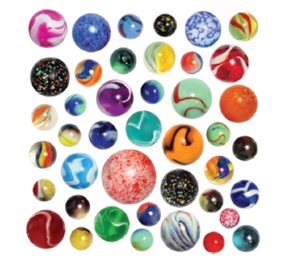
\includegraphics[width=4.04487in,height=1.57069in]{media/image24.png}
%Construir uma imagem semelhante a essa e nessa ilustração deve-se colocar:
%Colocar no lugar de 27 o 37 e no lugar de 65 o 75.
%Colocar no lugar de 78 o 83.

\begin{escolha}
\item Quantos quilogramas tem a caixa A?

\matlinhas{3}

\coment{75 -- 37 = 38 kg}

\item Sabendo a massa da caixa A, é possível encontrar a da caixa B? Se sim,
  calcule qual a massa da caixa B em quilogramas.

\matlinhas{3}

\coment{O cálculo é possível.

83 -- 37 = 46 Kg

Professor, comece a explorar o conceito de igualdade e, aos poucos, os conceitos primários de equações.}
\end{escolha}

%
\includegraphics[width=3.00278in,height=1.75833in]{media/image25.png}

\num{7} João possui uma distribuidora de ovos e acabou de receber 14 caixas
com 300 ovos cada uma. Para que João venda essa mercadoria, ele faz
embalagens com 12 ovos cada uma. Quantas embalagens João conseguirá
fazer para colocar à venda utilizando os ovos que acabou de receber em
sua loja?

%https://img.freepik.com/fotos-gratis/ovos-na-superficie-rosa_58702-1950.jpg?w=1060\&t=st=1677435684~exp=1677436284~hmac=6c6204dcded4c4d80a06169fee49d53df4b2636105a2c7b3dbe5365007ceae9a

\matlinhas{3}

\coment{(14 x 300):12 = 350 embalagens com 12 ovos cada uma.

Professor, sempre escreva a expressão formada pela interpretação do
enunciado, pois, assim, os alunos compreendem com mais clareza a transformação de textos em linguagem
matemática.}

\num{8} Brenda se deparou com uma divisão em sua prova de matemática. Para
esse cálculo, tínhamos 5.654 como dividendo e 24 como divisor. Sabendo-se
que Brenda acertou essa questão, qual foi o quociente encontrado por ela?

\matlinhas{4}

\coment{5.664 : 24 = 236.

Explore também divisões com dividendos maiores.}

\num{9} O pai de Pedro propôs um grande desafio para ele. O desafio
consistia em o pai fornecer uma conta com um número escondido e o filho descobrir qual seria esse número secreto. Ajude Pedro com esse
desafio e encontre o número que está escondido pelo quadrado.

%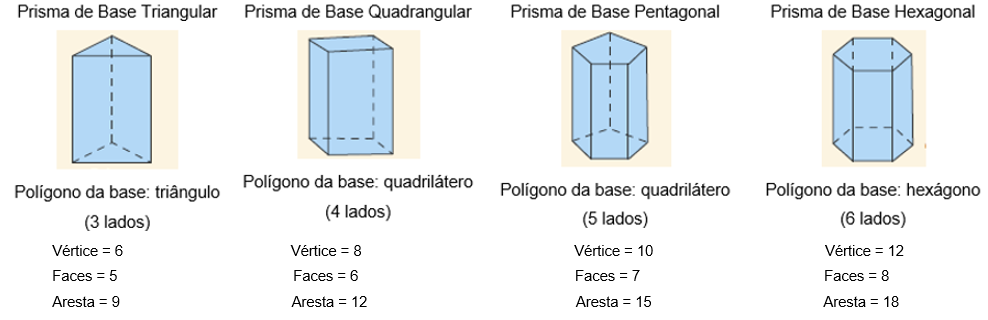
\includegraphics[width=1.85000in,height=1.43762in]{media/image26.png}
%Trocar estrela por um quadrado e colocar a conta acima como se estivesse em uma folha de caderno.

\coment{Realizando a conta de subtração, percebe-se facilmente que o número escondido pelo quadrado é o algarismo 1.}

\num{10} A mãe de Beatriz comprou uma caixa de bombons para presentear seus
quatro filhos. Na caixa os bombons estavam distribuídos em 3 fileiras
com 12 bombons em cada. Se ela irá dividir a quantidade total de bombons
igualmente entre seus filhos, quantos bombons Beatriz receberá?

\matlinhas{3}

\coment{(3 x 12) : 4 = 9 bombons para cada um de seus filhos.}

\colorsec{Treino}

\num{1} Verificando algumas atividades realizadas na escola no ano anterior
Gustavo se deparou com a seguinte conta em que um dos números estava
coberto por um retângulo.

%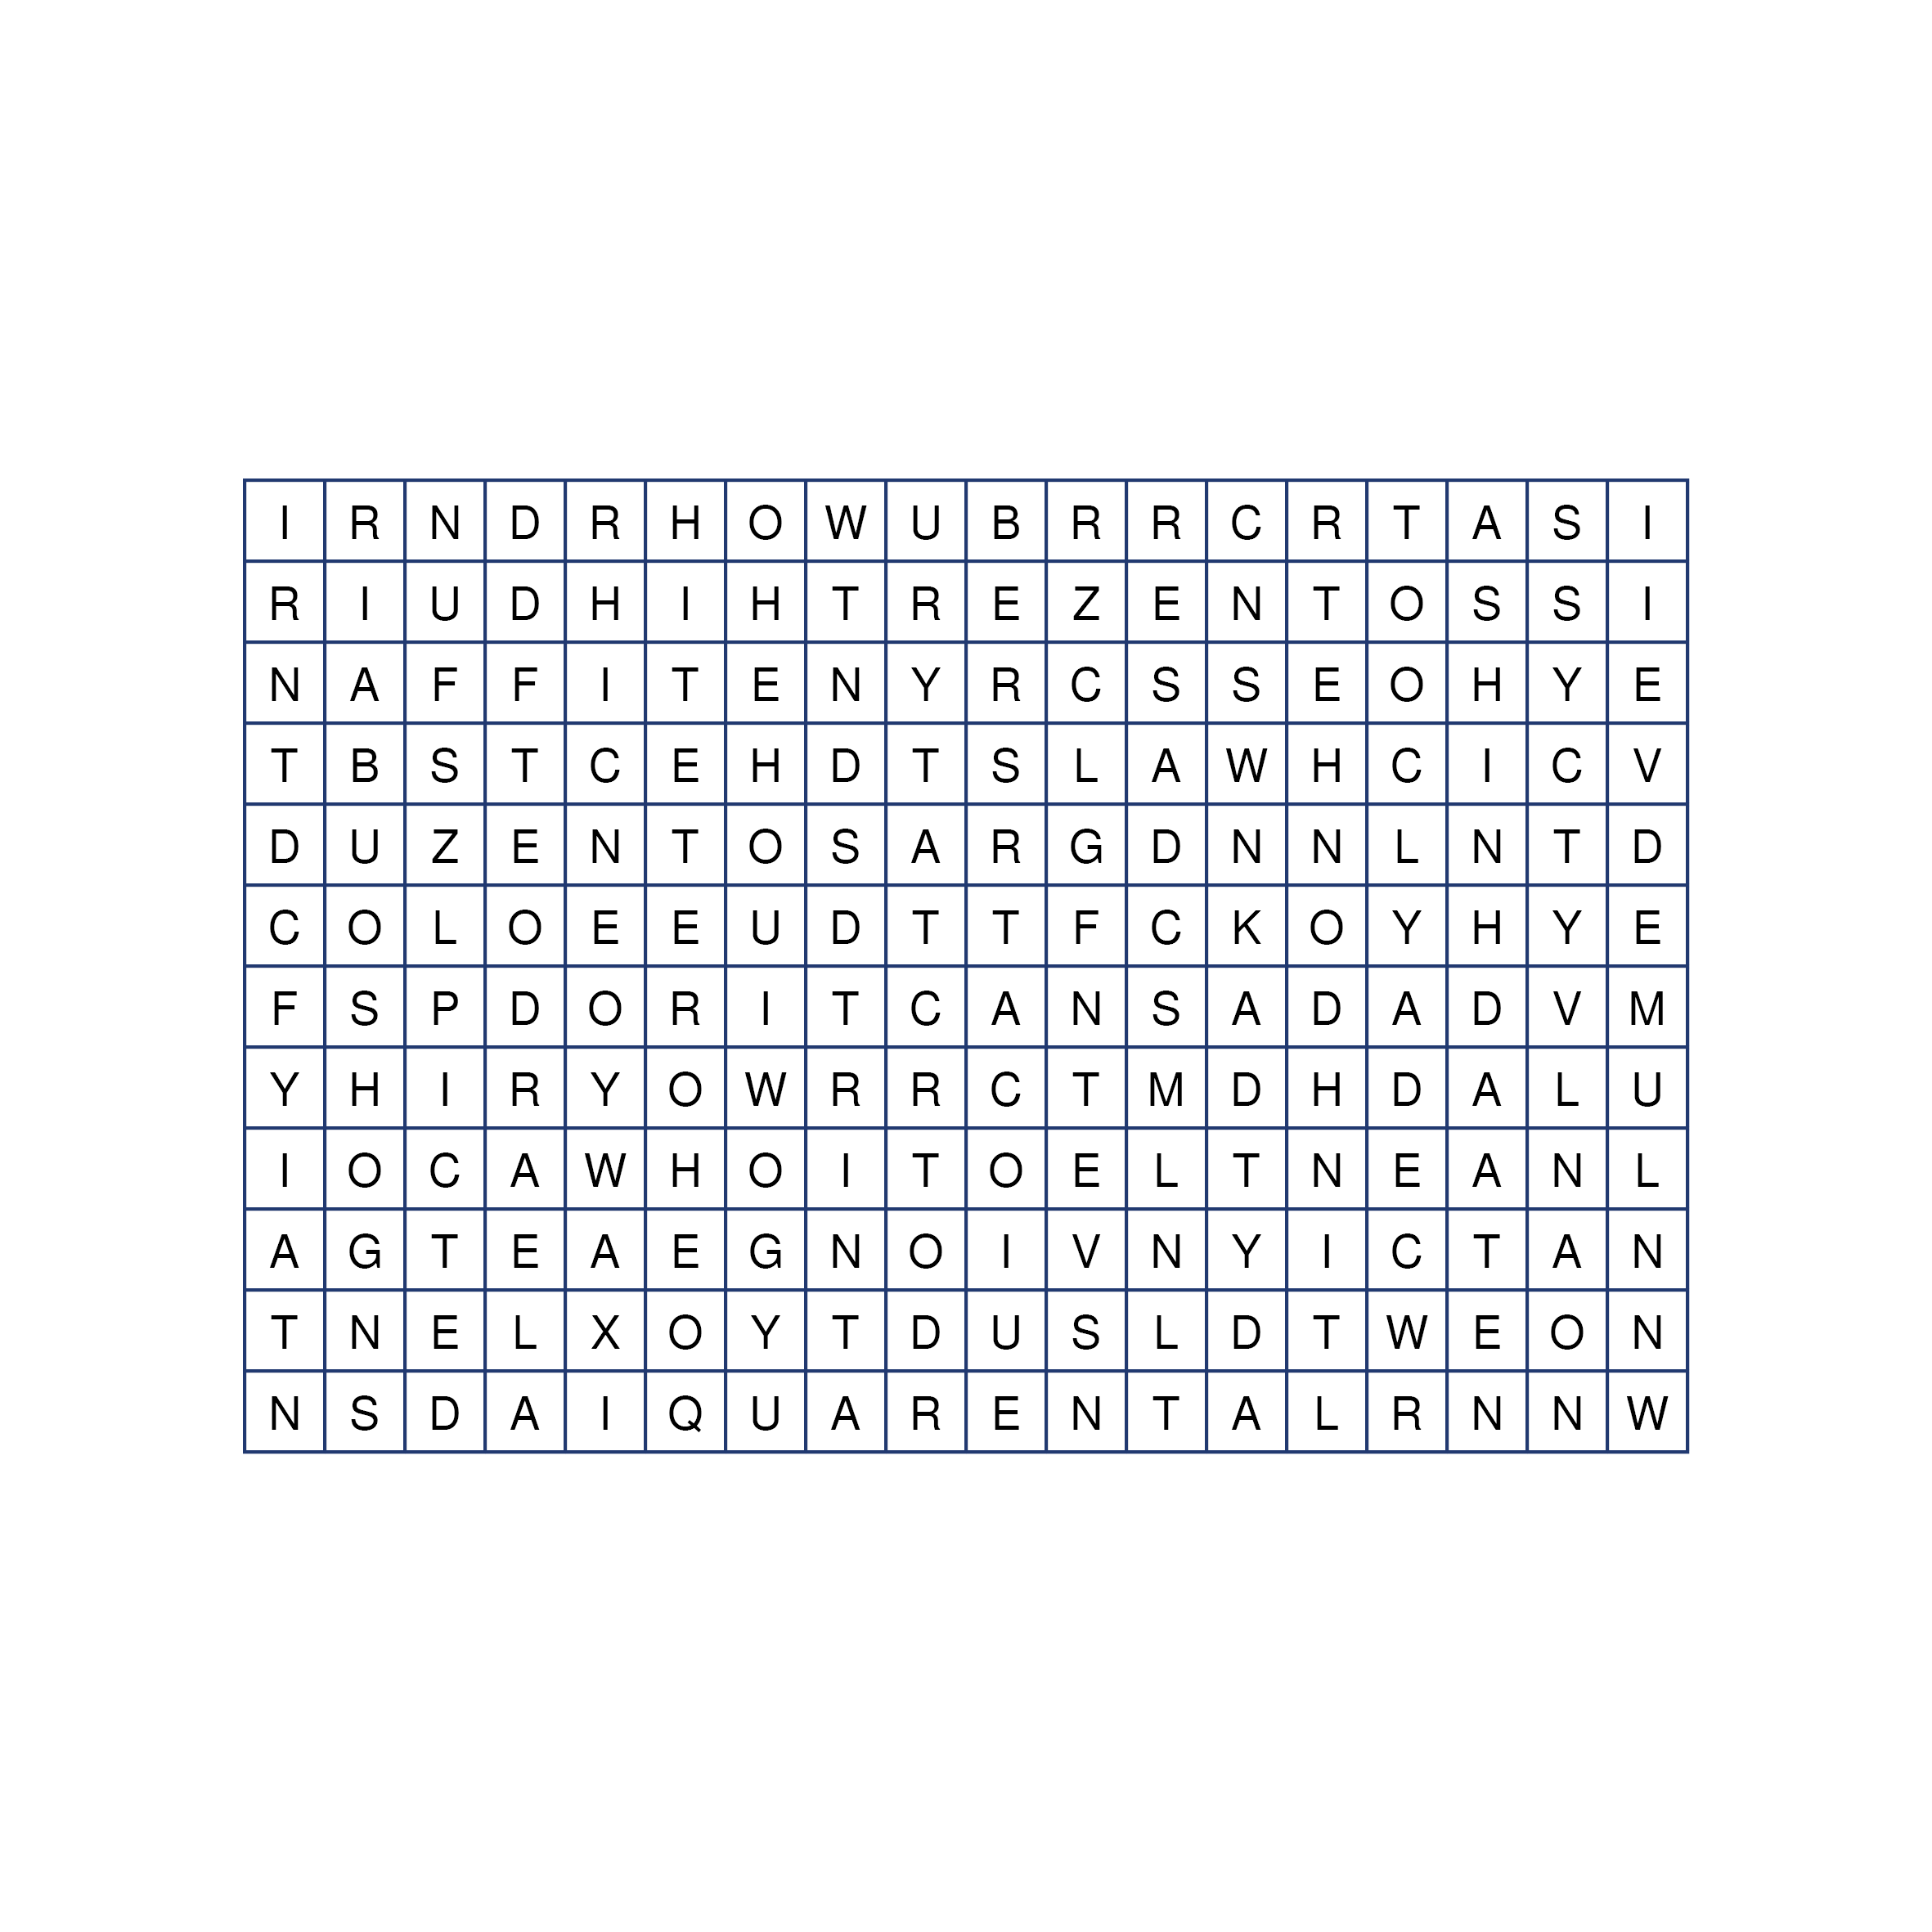
\includegraphics[width=5.39213in,height=1.80849in]{media/image27.png}
%Fazer uma ilustração nos moldes da acima e nela, trocar o número 178 pelo número 105

Gustavo ficou curioso e resolveu refazer a atividade para descobrir o
número que faltava e, após alguns minutos, conseguiu descobrir. Qual o número que Gabriel encontrou?

\begin{escolha}
\item
  128
\item
  312
\item
  158
\item
  256
\end{escolha}

\coment{SAEB: Calcular o resultado de adições ou subtrações envolvendo números naturais de até 6 ordens.
Não há correspondência com a BNCC do quinto ano.

a) Incorreta. Se  o número escondido fosse 128, o resultado seria 289.
b) Correta. 417 -- 105 = 312.
c) Incorreta. Se  o número escondido fosse 158, o resultado seria 259.
d) Incorreta. Se  o número escondido fosse 256, o resultado seria 161.}

\num{2} Isac estava conferindo o estoque de mercadorias de sua loja e
percebeu que, inicialmente, ele tinha 200 peças; depois, vendeu 2 caixas com peças para Carlos.

Em cada uma das caixas vendidas, havia um pacote com 5 unidades de peças e dois
pacotes com 7 peças.

Para saber a quantidade de peças que restavam no estoque Isac fez a
seguinte anotação:

\begin{quote}
200 -- 2 x (1 x 5 + 2 x 7)
\end{quote}

O resultado dessa expressão era exatamente igual à quantidade de peças
que restavam em seu estoque após a venda para Carlos. Qual é a
quantidade de peças que Isac tem agora em seu estoque?

\begin{escolha}
\item
  72
\item
  94
\item
  126
\item
  162
\end{escolha}

\coment{SAEB: Calcular o resultado de multiplicações ou divisões envolvendo números naturais de até 6 ordens.
Não há correspondência com a BNCC do quinto ano.

a) Incorreta. Para restarem 72 peças, teriam de ter sido vendidas 128.
b) Incorreta. Para restarem 94 peças, teriam de ter sido vendidas 106.
c) Incorreta. Para restarem 126 peças, teriam de ter sido vendidas 74.
d) 200 -- 2 x (1 x 5 + 2 x 7) = 200 -- 38 = 162 peças.}

\num{3} Um grande espetáculo chegou à cidade em que Rafael mora e, logo, uma fila
enorme se formou com pessoas querendo assistir. Os
ingressos começaram a ser vendidos e as pessoas começaram a entrar no
recinto. Em certo instante, sabia-se que 540 pessoas já tinham
entrado e que a capacidade máxima por espetáculo era de 1.200 pessoas. Como ainda temos 932 pessoas na fila, quantas pessoas não
conseguirão entrar para assistir à atração?

\begin{escolha}
\item
  268
\item
  272
\item
  294
\item
  1.440
\end{escolha}

\coment{SAEB: Resolver problemas de adição ou de subtração, envolvendo números naturais de até 6 ordens, com os significados de juntar, acrescentar, separar, retirar, comparar ou completar.
Não há correspondência com a BNCC do quinto ano.

a) Incorreta. Para restarem 268 pessoas na fila, deveriam estar aguardando 928 pessoas.
b) Correta.
1.200 -- 540 = 660.
932 -- 660 = 272 pessoas não conseguirão assistir a essa sessão.
c) Incorreta. Para restarem 294 pessoas na fila, deveriam estar aguardando 954 pessoas.
d) Incorreta. Para restarem 1.440 pessoas na fila, deveriam estar aguardando 2.100 pessoas.}


\chapter{3. Sequências}

\colorsec{Habilidades do SAEB}

\begin{itemize}
\item Inferir ou descrever atributos ou propriedades comuns que os elementos
que constituem uma sequência recursiva de números naturais apresentam.

\item Inferir o padrão ou a regularidade de uma sequência de números
naturais ordenados, objetos ou figuras.

\item Inferir os elementos ausentes em uma sequência de números naturais
ordenados, objetos ou figuras.
\end{itemize}

\coment{Professor, durante este módulo, explore bastante a percepção de seus
alunos, deixando realmente durante a algum tempo que eles tentem
descobrir a lógica de cada sentença, possibilitando, assim, que consigam descobrir os próximos números de cada uma. Esse é um conceito essencial
para estimular a criatividade e encontrar regras ``escondidas'' entre os números.}

\conteudo{Uma sequência ou sucessão é um conjunto numérico ordenado, em que há sempre uma lógica de formação e continuidade.

Exemplos:

\begin{itemize}
\item
  A escalação de um time de futebol de salão em ordem alfabética:
Alan; Bruno, Fernando, Igor, Tácio.

\item
  Sequência de números naturais pares:
(0; 2; 4; 6; 8; 10; 12; ...)
\end{itemize}

Podemos ainda classificar as sequências quanto ao número de elementos:

\begin{itemize}
\item
  Finitas: Sequências que apresentam um número de termos bem definido.
  ou seja: 10 termos, 20 termos, 8 termos.
\item
  Infinitas: Sequências que apresentam infinitos números de termos como é o caso da sequência dos números naturais.
\end{itemize}

Ainda podemos classificar as sequências em:

\begin{itemize}
\item
  Crescentes: aquelas em que cada termo sucessor é maior que seu antecessor.
Exemplo: (5, 10, 15, 20, 25)

\item
  Decrescentes: aquelas em que cada termos sucessor sempre é menor do que seu antecessor.
Exemplo: (9, 7, 5, 3)
\end{itemize}
}

\colorsec{Atividades}

\num{1} Observe as sequências dadas e determine, sem fazer desenhos, a
quantidade de bolinhas que a figura 8 de cada sequência terá.

\begin{escolha}
\item\preencher\coment{25} bolinhas

%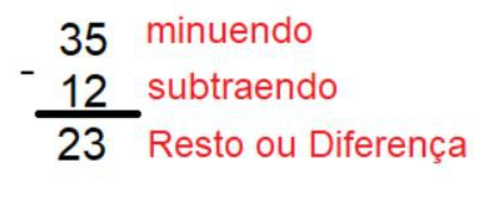
\includegraphics[width=4.09202in,height=0.85841in]{media/image28.png}
%Construir uma figura como a acima nos padrões cores do projeto

\matlinhas{2}

\coment{(4; 7; 10; 13; 16; 19; 22; 25) ou (8 x 3) + 1 = 25}

\item\preencher\coment{24} bolinhas

%
\includegraphics[width=2.38354in,height=0.81674in]{media/image29.png}
%Construir uma figura como a acima nos padrões cores do projeto

\matlinhas{2}

\coment{(3; 6; 9; 12; 15; 18; 21; 24) ou 8 x 3 = 24}

\item\preencher\coment{32} bolinhas

%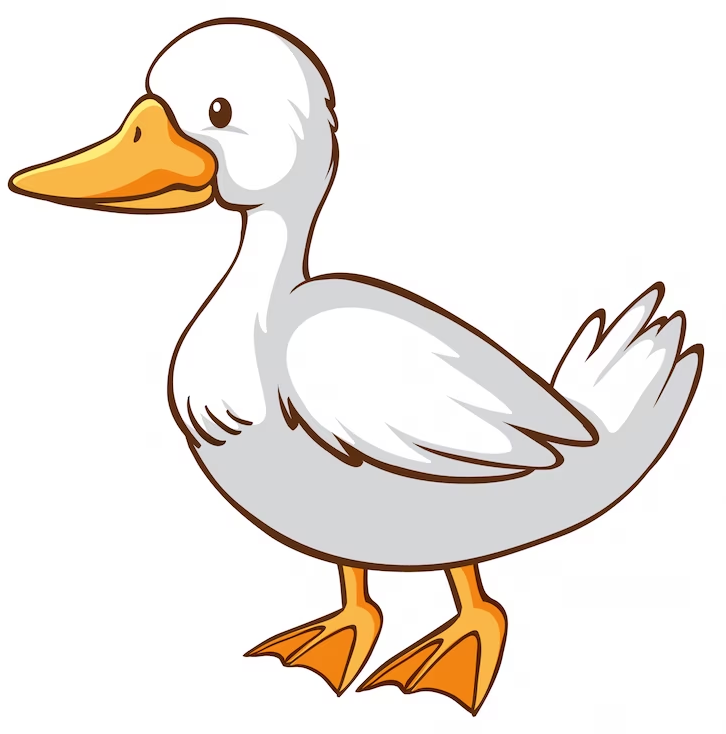
\includegraphics[width=2.38354in,height=0.85007in]{media/image30.png}
%Construir uma figura como a acima nos padrões cores do projeto.

\matlinhas{2}

\coment{(4; 8; 12; 16; 20; 24; 28; 32) ou 8 x 4 = 32}

\item\preencher\coment{40} bolinhas

%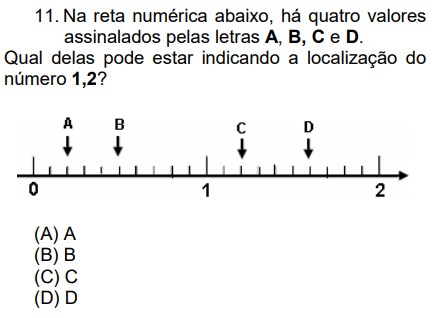
\includegraphics[width=2.35854in,height=0.94175in]{media/image31.png}
%Construir uma figura como a acima nos padrões cores do projeto

\matlinhas{2}

\coment{(5; 10; 15; 20; 25; 30; 35; 40) ou 8 x 5 = 40}
\end{escolha}

\num{2} Genivaldo, um adulto de 45 anos, adora participar de corridas de
rua. Em uma delas ele correu com mais 49 pessoas e utilizou uma camiseta
de identificação com o número 28.

\begin{escolha}
\item
  Qual dos números que estão no texto acima representa uma
  quantidade? \preencher \coment{49}
\item
  Qual dos números que estão no texto acima representa um
  código? \preencher \coment{28}
\item
  Qual dos números que estão no texto acima representa uma
  medida? \preencher \coment{45}
\item
  Represente os números presentes no texto na forma de uma sequência
  decrescente e diga se ela é finita ou infinita.

\linhas{1}
\end{escolha}

\coment{a) 49, pois representa a quantidade de pessoas que correrem além de Genivaldo.
b)  28, pois é o código de identificação da camiseta de Genivaldo.
c)  45, pois mede a quantidade de anos que Genivaldo tem.
d)  (49; 45; 28), que é uma sequência finita.}

\num{3} Encontre o número pedido em cada item a seguir.

\begin{escolha}
\item
  O sucessor de 3.089: \preencher\coment{3.090}
\item
  O antecessor de 4.301: \preencher\coment{4.300}
\item
  O sucessor e antecessor do número 3.259: \preencher\coment{3.258} e \preencher\coment{3.260}
\end{escolha}

\coment{
a)  3.090 aparece, em sequência crescente, após 3.089.
b)  4.300 aparece, em sequência crescente, antes de 4.301.
c)  Antecessor: 3.258. Sucessor: 3.260. São os números que, em sequência crescente, aparecem antes e depois de 3.259.

Professor, explore bastante os conceitos de sucessor e antecessor com
seus alunos, pois isso facilitará muitos entendimentos em módulos e anos futuros.}

\num{4} Ana Clara encontrou o papel representado a seguir entre os cadernos de seu irmão mais velho.

%
\includegraphics[width=3.30833in,height=2.17391in]{media/image15.png}
%Na folha colocar bem grande a sequência :(23; 60; 97; 134; ...)
%https://img.freepik.com/vetores-gratis/vetor-de-fundo-de-design-de-pedaco-de-papel-rasgado_1055-13108.jpg?w=900\&t=st=1677434705~exp=1677435305~hmac=787f679840c02b57af4cb87ef851030bb83880366602641e4486462d6d3553f8

Ela ficou muito curiosa, pois entendeu que essa era uma sequência
numérica e queria encontrar qual o próximo número dela.

Ajude Ana Clara a descobrir qual é o próximo número da sequência e o escreva no espaço que segue.

\linhas{1}

\coment{A sequência foi montada sempre somando 37 ao número anterior para
encontrar o próximo. Portanto, o próximo número da sequência será: 134 + 37 = 171.}

\num{5} Utilizando apenas os algarismos 2, 3 e 4, escreva a sequência de
todos os números com 3 algarismos que podemos formar utilizando esses
três números sem que eles apareçam mais de uma vez em cada número.

\linhas{3}

\coment{(234, 243, 324, 342, 423, 432)}

\num{6} O Pai de André montou a sequência de figuras a seguir.

%
\includegraphics[width=4.30871in,height=1.10010in]{media/image32.png}
%Construir uma figura como essa nos moldes e cores do projeto. A figura tem que seguir o mesmo padrão;

Então, ele disse ao filho que o levaria ao cinema caso ele acertasse
qual seria o décimo termo dessa sequência. André, muito empolgado, começou a
pensar e logo deu a resposta a seu pai. O pai analisou a resposta e
disse que estava correta.

Qual a resposta que André deu a seu pai sobre qual era o décimo elemento da sequência?

\linhas{3}

\coment{Só teremos triângulos em múltiplos de 3 e, portanto, como 10 não é um
múltiplo de 3, a figura será um quadrado.

Professor, é possível que o aluno continue a sequência com desenhos até
chegar à resposta. Não há problema algum e é muito válido, pois assim entenderá a lógica envolvida.}

\num{7} Relembre os conceitos de números naturais pares e ímpares e, em
seguida, resolva a atividade.

\begin{escolha}
\item
  Escreva os 10 primeiros números naturais pares em sequência crescente.
  Essa sequência é finita ou infinita? Como ela é formada?

\matlinhas{3}

\coment{(0; 2; 4; 6; 8; 10; 12; 14; 16; 18). Essa é uma sequência finita e sempre
somamos 2 ao termo anterior para encontrar o próximo.}

\item
  Escreva os 12 primeiros números naturais ímpares em sequência
  crescente. Essa sequência e finita ou infinita? Como ela é formada?

\matlinhas{3}

\coment{(1; 3; 5; 7; 9; 11; 13; 15; 17; 19; 21; 23). Essa é uma sequência finita
e sempre somamos 2 ao termo anterior para encontrar o próximo.

Professor, explorar como os alunos o conceito de que, na sequência dos
números naturais, após um número par sempre vem um numero ímpar; ou seja, eles se intercalam.}
\end{escolha}

\num{8} Estudando com a sua filha para a prova de matemática da semana
seguinte, Laura propõe a Luísa o seguinte exercício:

Escreva uma sequência de 6 números que aumentam de 2 em 2 unidades,
começando pelo número nove mil e novecentos e noventa e nove.

Ajude Luísa a resolver esse exercício, escrevendo os seis números pedidos no espaço demarcado.

\linhas{2}

\coment{(9.999; 10.001; 10.003; 10.005; 10.007; 10.009)}

\num{9} Monte cada uma das sequências a seguir, com seis números cada uma,
prestando muita atenção em qual número começam e qual a regra elas devem
seguir.

\begin{enumerate}
\item
  Sequência de números que começa no 22 e cujos números aumentam de 9 em 9 unidades.

\linhas{2}

\item
  Sequência de números que começa no 30 e cujos números aumentam de 40 em 40 unidades.

\linhas{2}

\item
  Sequência de números que começa no 220 e cujos números diminuem de 5 em 5 unidades.

\linhas{2}
\end{enumerate}

\coment{a) (22; 31; 40; 49; 58; 67);
b)  (30; 70; 110; 150; 190; 230);

c) (220; 215; 210; 205; 200; 195).}

\num{10} Observe as sequências apresentadas e complete-as com os números que estão faltando.

\begin{longtable}[]{@{}llllll@{}}
\toprule
19 & 22 & 25 & \rosa{28} & \rosa{31} & 34\tabularnewline
\bottomrule
\end{longtable}

\begin{longtable}[]{@{}llllll@{}}
\toprule
198 & 194 & \rosa{190} & 186 & \rosa{182} & \rosa{178}\tabularnewline
\bottomrule
\end{longtable}

\coment{
(19; 22; 25; 28; 31; 34) - os números aumentam de 3 em 3.
(198; 194; 190; 186; 182; 178) - os números diminuem de 4 em 4.}

\colorsec{Treino}

\num{1} Observe a sequência a seguir e marque a alternativa que corresponde ao número de elementos que a figura 6 terá.

%Construir uma figura conforme a abaixo nos padrões do projeto
%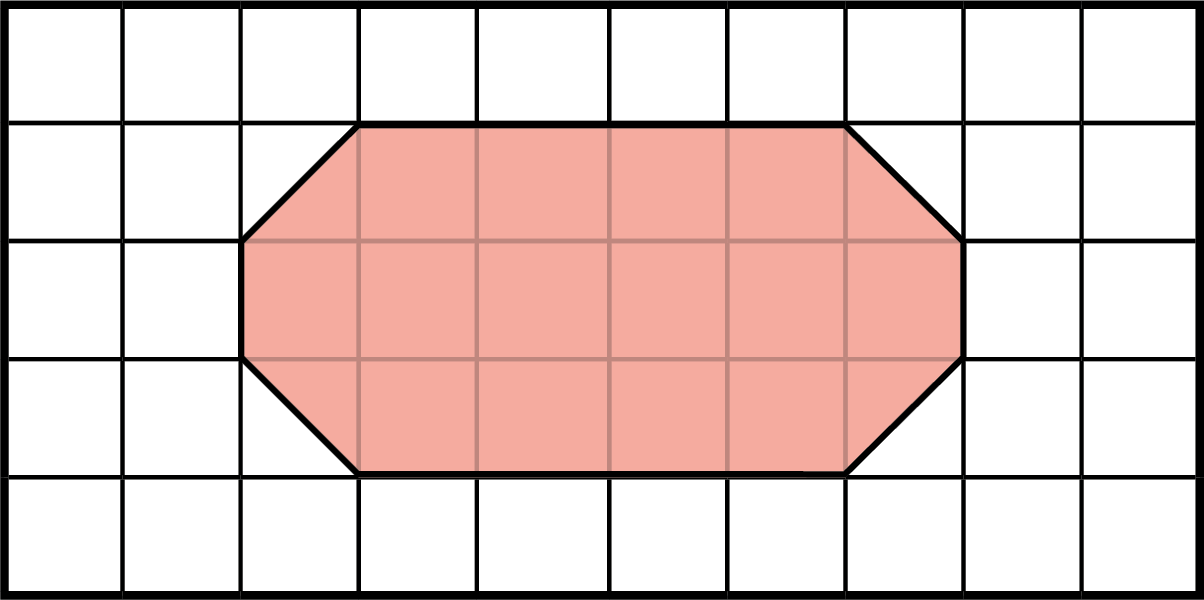
\includegraphics[width=4.75875in,height=1.35012in]{media/image33.png}

\begin{escolha}
\item
  25
\item
  30
\item
  35
\item
  42
\end{escolha}

\coment{SAEB: Inferir os elementos ausentes em uma sequência de números naturais ordenados, objetos ou figuras.
Não há correspondência com a BNCC do quinto ano.

a) Incorreta. 25 não é o resultado de 6, multiplicado por ele mesmo, mais ele mesmo.
b) Incorreta. 30 será o número de elementos da figura 5.
c) Incorreta. 35 não faz parte da sequência, em nenhuma posição.
d) Correta. (2; 6; 12; 20; 30; 42).


Professor, a sequência é dada por n² + n =
6² + 6 = 42 (sendo n o número da figura. 1² + 1 = 2; 2² + 2 = 6; 3² + 2 = 12; 4² + 4 = 20...)}

\num{2} Analise com muita atenção a sequência apresentada e assinale a
alternativa que traz, de acordo com o padrão de formação, a classificação em crescente ou decrescente e
em finita ou infinita.

\begin{quote}
(66, 55, 44, 33, 22, 11)
\end{quote}

\begin{escolha}
\item
  Crescente e infinita.
\item
  Crescente e finita.
\item
  Decrescente e finita.
\item
  Decrescente e infinita.
\end{escolha}

\coment{SAEB: Inferir ou descrever atributos ou propriedades comuns que os elementos que constituem uma sequência recursiva de números naturais apresentam.
Não há correspondência com a BNCC do quinto ano.

a) Incorreta. A sequência é decrescente e finita, ao contrário do que se afirma.
b) Incorreta. A sequência é realmente finita, mas decrescente.
c) Correta. Pela análise da sequência dada, percebemos que ela é finita e
decrescente.
d) Incorreta. A sequência é realmente decrescente, mas finita.

\num{3} Dois aplicativos exigem uma senha numérica para serem acessados.
Breno
criou a senha 6.081 para o primeiro e, para o segundo, utilizou como senha
o sucessor do sucessor do número escolhido para a primeira senha. Qual a
senha utilizada por Breno para o segundo aplicativo?

\begin{escolha}
\item
  6.079
\item
  6.080
\item
  6.082
\item
  6.083
\end{escolha}

\coment{SAEB: Inferir o padrão ou a regularidade de uma sequência de números naturais ordenados, objetos ou figuras.
Não há correspondência com a BNCC do quinto ano.

a) Incorreta. 6.079 é o antecessor do antecessor de 6.081.
b) Incorreta. 6.080 é o antecessor de 6.081.
c) Incorreta. 6.082 é o sucessor de 6.081.
d) Correta. Sucessor do sucessor de 6.081 = 6.081 +1 +1 = 6.083.}

\chapter{4. Medindo o mundo}

\coment{Habilidade da BNCC: EF05MA19.}

\colorsec{Habilidades do SAEB}

\begin{itemize}
\item Reconhecer a unidade de medida ou o instrumento mais apropriado para
medições de comprimento, área, massa, tempo, capacidade ou temperatura.

\item Estimar/inferir medida de comprimento, capacidade ou massa de objetos,
utilizando unidades de medida convencionais ou não ou medir comprimento,
capacidade ou massa de objetos.

\item Explicar que o resultado de uma medida depende da unidade de medida utilizada.

\item Resolver problemas que envolvam medidas de grandezas (comprimento,
massa, tempo e capacidade) em que haja conversões entre as unidades mais
usuais.

\item Determinar o horário de início, o horário de término ou a duração de
um acontecimento.
\end{itemize}

\conteudo{Professor, durante todo este módulo, trabalhe com os alunos outras
unidades e medidas não tratadas nos exercícios, como
jardas, alqueires, hectares, milhas, milhas náuticas, medidas de som, entre outras.}

%Construir os quadros abaixo seguindo o padrão de cores do material.
%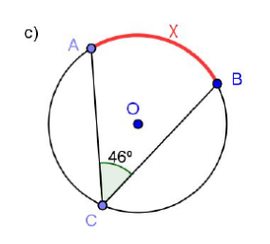
\includegraphics[width=4.23370in,height=2.06685in]{media/image34.png}
%
\includegraphics[width=4.25870in,height=1.18344in]{media/image35.png}

\colorsec{Atividades}

\num{1} Relacione as quantidades que estão na coluna 1 com a leitura correta correspondente.

\begin{multicols}{2}
\red{1,935 kg} 

\red{2,340 km} 

\red{0,400 g} 

\red{0,35 m} 

\blue{Trinta e cinco centímetros.}

\blue{Um quilo e novecentos e trinta e cinco gramas.}

\blue{Dois quilômetros e trezentos e quarenta metros.}

\blue{Quatrocentos miligramas.}
\end{multicols}


\coment{
1.935 kg = um quilo e novecentos e trinta e cinco gramas.

2,340 km = Dois quilômetros e trezentos e quarenta metros.

0,400 g = quatrocentos miligramas.

0,35 m = trinta e cinco centímetros.}

\num{2} Relacione a primeira com a segunda coluna levando em conta qual
valor pode corresponder à medida mostrada.

\begin{multicols}{2}

Altura aproximada de uma porta (\coment{2 m})

Comprimento aproximado de um lápis (\coment{20 cm})

Comprimento médio de um quarteirão (\coment{90 m})

Comprimento aproximado de uma quadra de basquete (\coment{30 m})

\columnbreak

20 cm
 
90 m

30 m
 
2 m
\end{multicols}

\coment{Professor, explore bastante com os alunos esse senso de tamanho, pois 
é um conceito extremamente importante para eles.}

\num{3} Pinte a opção que corresponde à capacidade total de líquido que
há em:

%Construir essas imagens no padrão e cores do projeto. Atenção aso textos pois são essenciais para a resolução.
%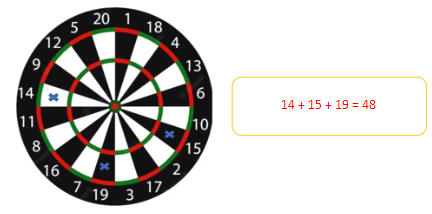
\includegraphics[width=4.17536in,height=3.42530in]{media/image36.png}

\coment{
2 unidades de limpador multiuso de 500 ml = 1 l

3 unidades de loção hidratante de 150 ml = 450 ml, que é menos que 0,5 l

4 unidades de água de coco de 330 ml = 1.320 ml = 1,32 l que é
menos do que 1,5 l

4 unidades de amaciante de roupas de 1 000 ml = 4 000 ml = 4 l, que é mais
do que 3,5 l}

\num{4} Débora decidiu estimar a medida do lápis com sua borracha.

%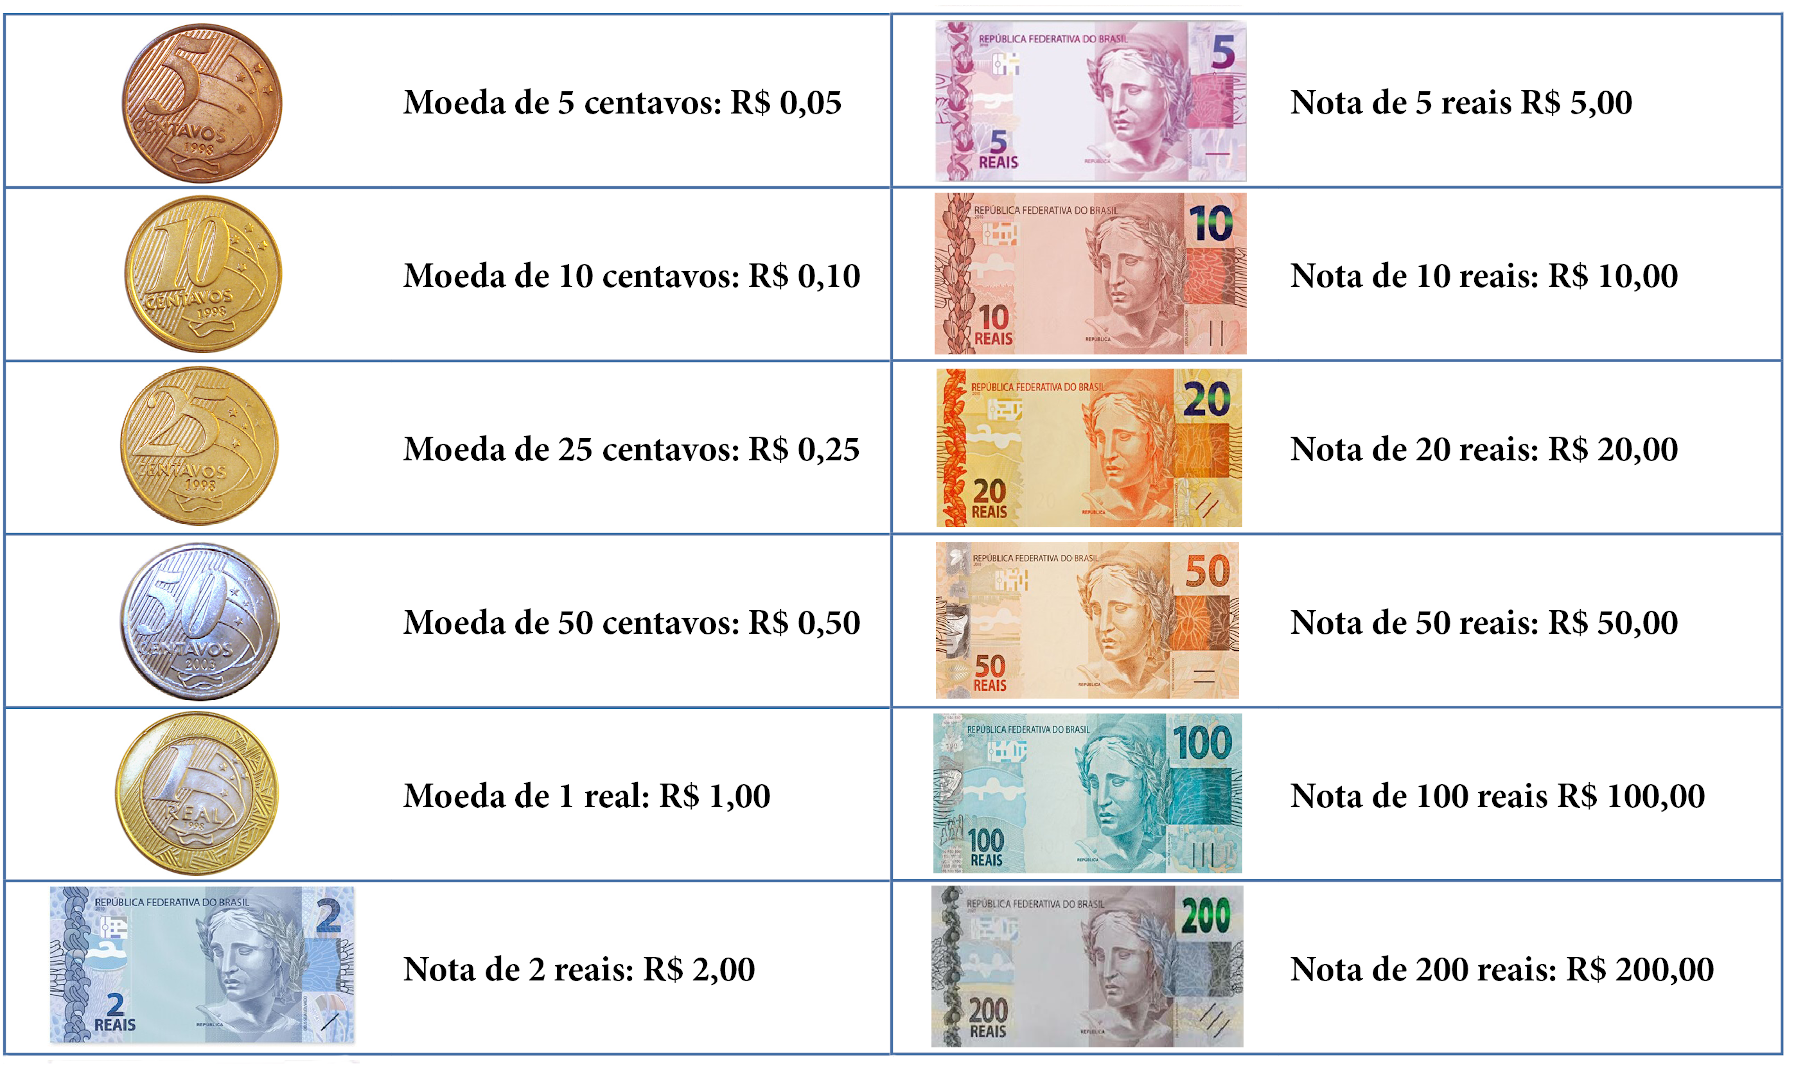
\includegraphics[width=3.84200in,height=1.23344in]{media/image37.png}
%Construir essa imagem nos padrões do projeto.
%O lápis e a borracha devem ter tamanhos de forma que no comprimento de um lápis caibam de 4 a 5 borrachas. O desenho é fundamental para a resolução dessa questão.

Quantas borrachas, considerando a figura dada, aproximadamente, mede o
lápis de Débora?

\begin{escolha}
\item
  Entre 2 e 3.
\item
  Entre 4 e 5.
\item
  Entre 6 e 7.
\item
  Mais que 9.
\end{escolha}

\coment{Resposta: B.
Através da percepção de comparação de comprimentos, percebe-se que. no
comprimento de um lápis. cabem cerca de 4 a 5 borrachas conforme a figura
dada.}

\num{5} Um dos brinquedos do parque de diversões permanente de uma cidade
proíbe que crianças com uma altura menor que 1,20 m possam brincar nessa
atração. Manoel mediu sua altura e ele está com 93 cm. Quanto ele
precisa crescer para poder realizar seu sonho de andar nesse brinquedo?

\matlinhas{2}

\coment{
1,20 m = 120 cm

120 -- 93 = 23 cm

Portanto, Manoel ainda precisará crescer 23 cm para que esteja apto a brincar
nessa atração.}

\num{6} Roberto está com sintomas de dor de garganta e sua mãe decidiu leválo ao
médico. Chegando lá, sua temperatura foi medida e a foto do termômetro
está a seguir.

%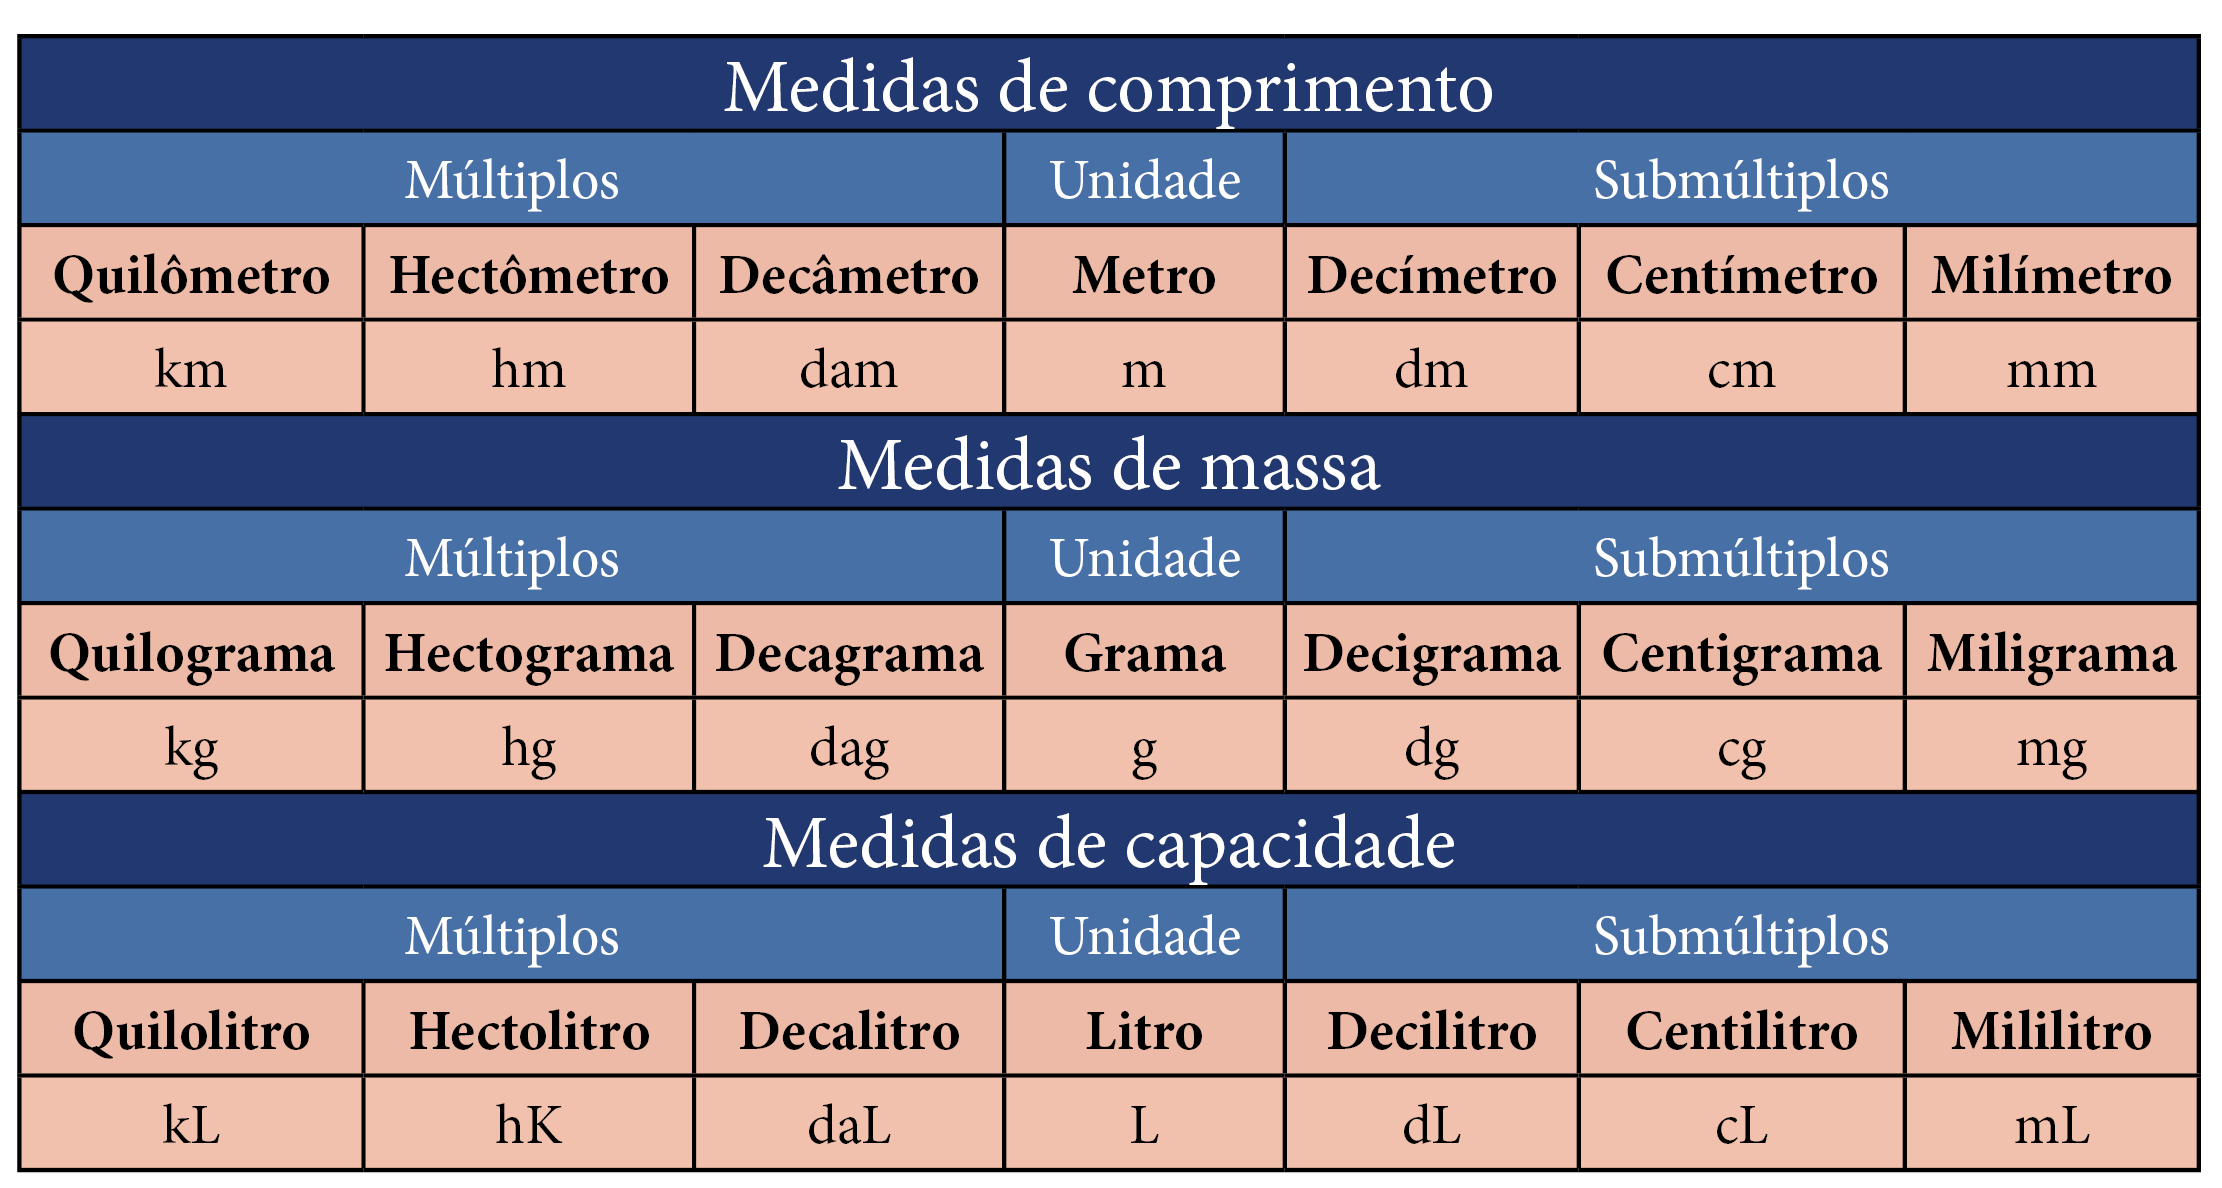
\includegraphics[width=3.15000in,height=1.59426in]{media/image38.png}
%https://img.freepik.com/vetores-gratis/elemento-termometro-digital-38-5-graus-celsius_53876-119949.jpg?w=1380\&t=st=1677436599~exp=1677437199~hmac=efddbcbdae2d4d75bd1e8476eee389a985a191d57800533acdff847111e69669

Analisando a imagem do termômetro, podemos concluir que a temperatura de
Roberto, naquele instante, era de quanto?

\coment{38,5° C.
Observando a figura percebemos que o termômetro está marcando exatamente
38,5° C}

\num{7} Dados da prefeitura de uma determinada cidade revelam que cada
habitante, em média, produz 500 g de lixo por dia. Quantas toneladas de lixo,
aproximadamente, são produzidas, por dia, nessa cidade, que
possui uma população de 28.165 habitantes?

\matlinhas{3}

\coment{28.165 x 500 = 14.082.500 g = 14.082,50 kg = 14,0825 toneladas.}

\num{8} Para a festa de aniversário de Arthur, seu pai encomendou 24
garrafas de refrigerante. Dessas garrafas, 10 continham, cada uma, 3
litros. Nas demais garrafas, havia dois litros em cada uma. Com base
nessas informações, responda ao que se pede.

\begin{escolha}
\item
  Qual a quantidade, em mililitros, encomendada pelo pai de Arthur?

\matlinhas{3}

\item
  Se cada pessoa consumiu exatamente 400 mililitros de refrigerante e
  todo o refrigerante foi consumido durante a festa, quantas pessoas
  foram ao aniversário de Arthur?

\matlinhas{2}
\end{escolha}

\coment{
a) (10 x 3) + (14 x 2) = 30 + 28 = 58 l = 58.000 ml.
b) 58.000 : 400 = 145 pessoas compareceram à festa.}

\num{9} O comprimento de uma escrivaninha é de 1,6 m. Quantos palmos,
aproximadamente, mede a escrivaninha se, em média, um palmo tem 23 cm?

\coment{Resposta: 7.

1,6 m = 160 cm

160 : 23 = 6,95 palmos. Aproximadamente 7 palmos.}

\num{10} Uma série de televisão proporciona episódios com duração de 45
minutos. Se Jorge terminou de assistir a um desses episódios às 18 horas, qual
foi o horário em que ele começou a assistir a esse episódio, considerando que tenha assistido
no início ao fim sem parar nenhuma vez?

\matlinhas{2}

\coment{Ele começou a assistir ao episódio às 17 horas e 15 minutos, pois, se a esse
horário somarmos a duração do episódio, que é de 45 minutos, teremos o
horário final, que foi às 18 horas.}

\section{Treino}

\num{1} Reinaldo foi contratado por uma empresa que possui um horário bem
rígido e semanal que deve ser cumprido corretamente. No período da manhã,
ele deve cumprir 4 horas e 30 minutos de trabalho. Qual será o horário em que
Reinaldo sairá para almoçar nesses dias?

\begin{longtable}[]{@{}lll@{}}
\toprule
& Entrada & Saída\tabularnewline
\midrule
\endhead
Manhã & 8:00 & ?\tabularnewline
Tarde & 14:00 & 17:30\tabularnewline
\bottomrule
\end{longtable}

\begin{escolha}
\item
  11:00
\item
  11:30
\item
  12:00
\item
  12:30
\end{escolha}

\coment{SAEB: Determinar o horário de início, o horário de término ou a duração de um acontecimento.
BNCC: EF05MA19 -- Resolver e elaborar problemas envolvendo medidas das grandezas comprimento,
área, massa, tempo, temperatura e capacidade, recorrendo a transformações entre as unidades
mais usuais em contextos socioculturais.}

a) Incorreta. Saindo a esse horário ele completará 3h de trabalho.
b) Incorreta. Saindo a esse horário ele completará 3h30min de trabalho.
c) Incorreta. Saindo a esse horário ele completará 4h de trabalho.
d) Correta. Como pela manhã ele entra às 8:00 e deve cumprir nesse período 4 horas e
meia de trabalho antes de sair para o almoço, conclui-se que ele sairá
para o almoço às 12:30.}

\num{2} Em uma receita médica que Marcela recebeu, o médico recomenda que ela tome um xarope 3
vezes ao dia e que, a cada vez, ela tome a quantidade de 10 ml. Isso deve se repetir durante 7
dias. Um frasco do remédio contém 100 ml. Sendo assim, qual a quantidade
de frascos que a mãe de Marcela terá que comprar para que todo o
tratamento seja concluído?

\begin{escolha}
\item
  1
\item
  2
\item
  3
\item
  4
\end{escolha}

\coment{SAEB: Reconhecer a unidade de medida ou o instrumento mais apropriado para medições de comprimento, área, massa, tempo, capacidade ou temperatura.
BNCC: EF05MA19 -- Resolver e elaborar problemas envolvendo medidas das grandezas comprimento,
área, massa, tempo, temperatura e capacidade, recorrendo a transformações entre as unidades
mais usuais em contextos socioculturais.

a) Incorreta. Um frasco contém 100 ml; menos do que a quantidade de que ela precisa.
b) Incorreta. Com a compra de 2 frascos faltará uma dose; ou seja, 10 ml.
c) Correta. 
3 x 10 x 7 = 210 ml. Como cada frasco contém 100 ml, ela terá que
comprar 3 frascos e haverá uma sobra de xarope.
d) Incorreta. Na compra de 4 frascos, um restará fechado e inutilizado; não há essa necessidade.}

\num{3} Vicente teve que fazer uma viagem para fechar um grande negócio. Seu
voo saiu do aeroporto às 10 horas e 42 minutos e chegou ao seu destino
às 14 horas e 8 minutos. Qual foi o tempo de duração do voo?

\begin{escolha}
\item
  12.300 segundos
\item
  9.542 segundos
\item
  5.364 segundos
\item
  2.500 segundos
\end{escolha}

\coment{SAEB: Determinar o horário de início, o horário de término ou a duração de um acontecimento.
BNCC: EF05MA19 -- Resolver e elaborar problemas envolvendo medidas das grandezas comprimento,
área, massa, tempo, temperatura e capacidade, recorrendo a transformações entre as unidades
mais usuais em contextos socioculturais.

a) Correta. 
Saída: 10 horas e 42 minutos;
Chegada: 14 horas e 8 minutos;
Tempo de voo: 3 horas e 26 minutos = 206 minutos = 12.300 segundos.
b) Incorreta. Trata-se de mais do que esse tempo.
c) Incorreta. Trata-se de mais do que o dobro desse tempo.
d) Incorreta. Trata-se de algo próximo de cinco vezes esse tempo mencionado.}

\chapter{5. Áreas, espaços, tamanhos}

\colorsec{Habilidades do SAEB}

\begin{itemize}
\item Medir ou comparar perímetro ou área de figuras planas desenhadas em
malha quadriculada.

\item Identificar horas em relógios analógicos ou associar horas em relógios
analógicos e digitais.

\item Resolver problemas que envolvam perímetro de figuras planas.

\item Resolver problemas que envolvam área de figuras planas.
\end{itemize}

\conteudo{Professor, explore bastante os conceitos de identificação de horas e
relógio analógico e também a utilização da malha quadriculada para
identificação do perímetro e de área de figuras planas.

Ampliação: é o processo que realizamos quando queremos aumentar algo (como figuras planas, por exemplo) sem que suas características essenciais
sejam alteradas.

A figura representada teve seus lados dobrados e manteve as mesmas
características. Observe.

%Fazer a figura a seguir sem marcar os ângulos e a primeira deve ter lado 3 cm e a segunda lado 6 cm.
%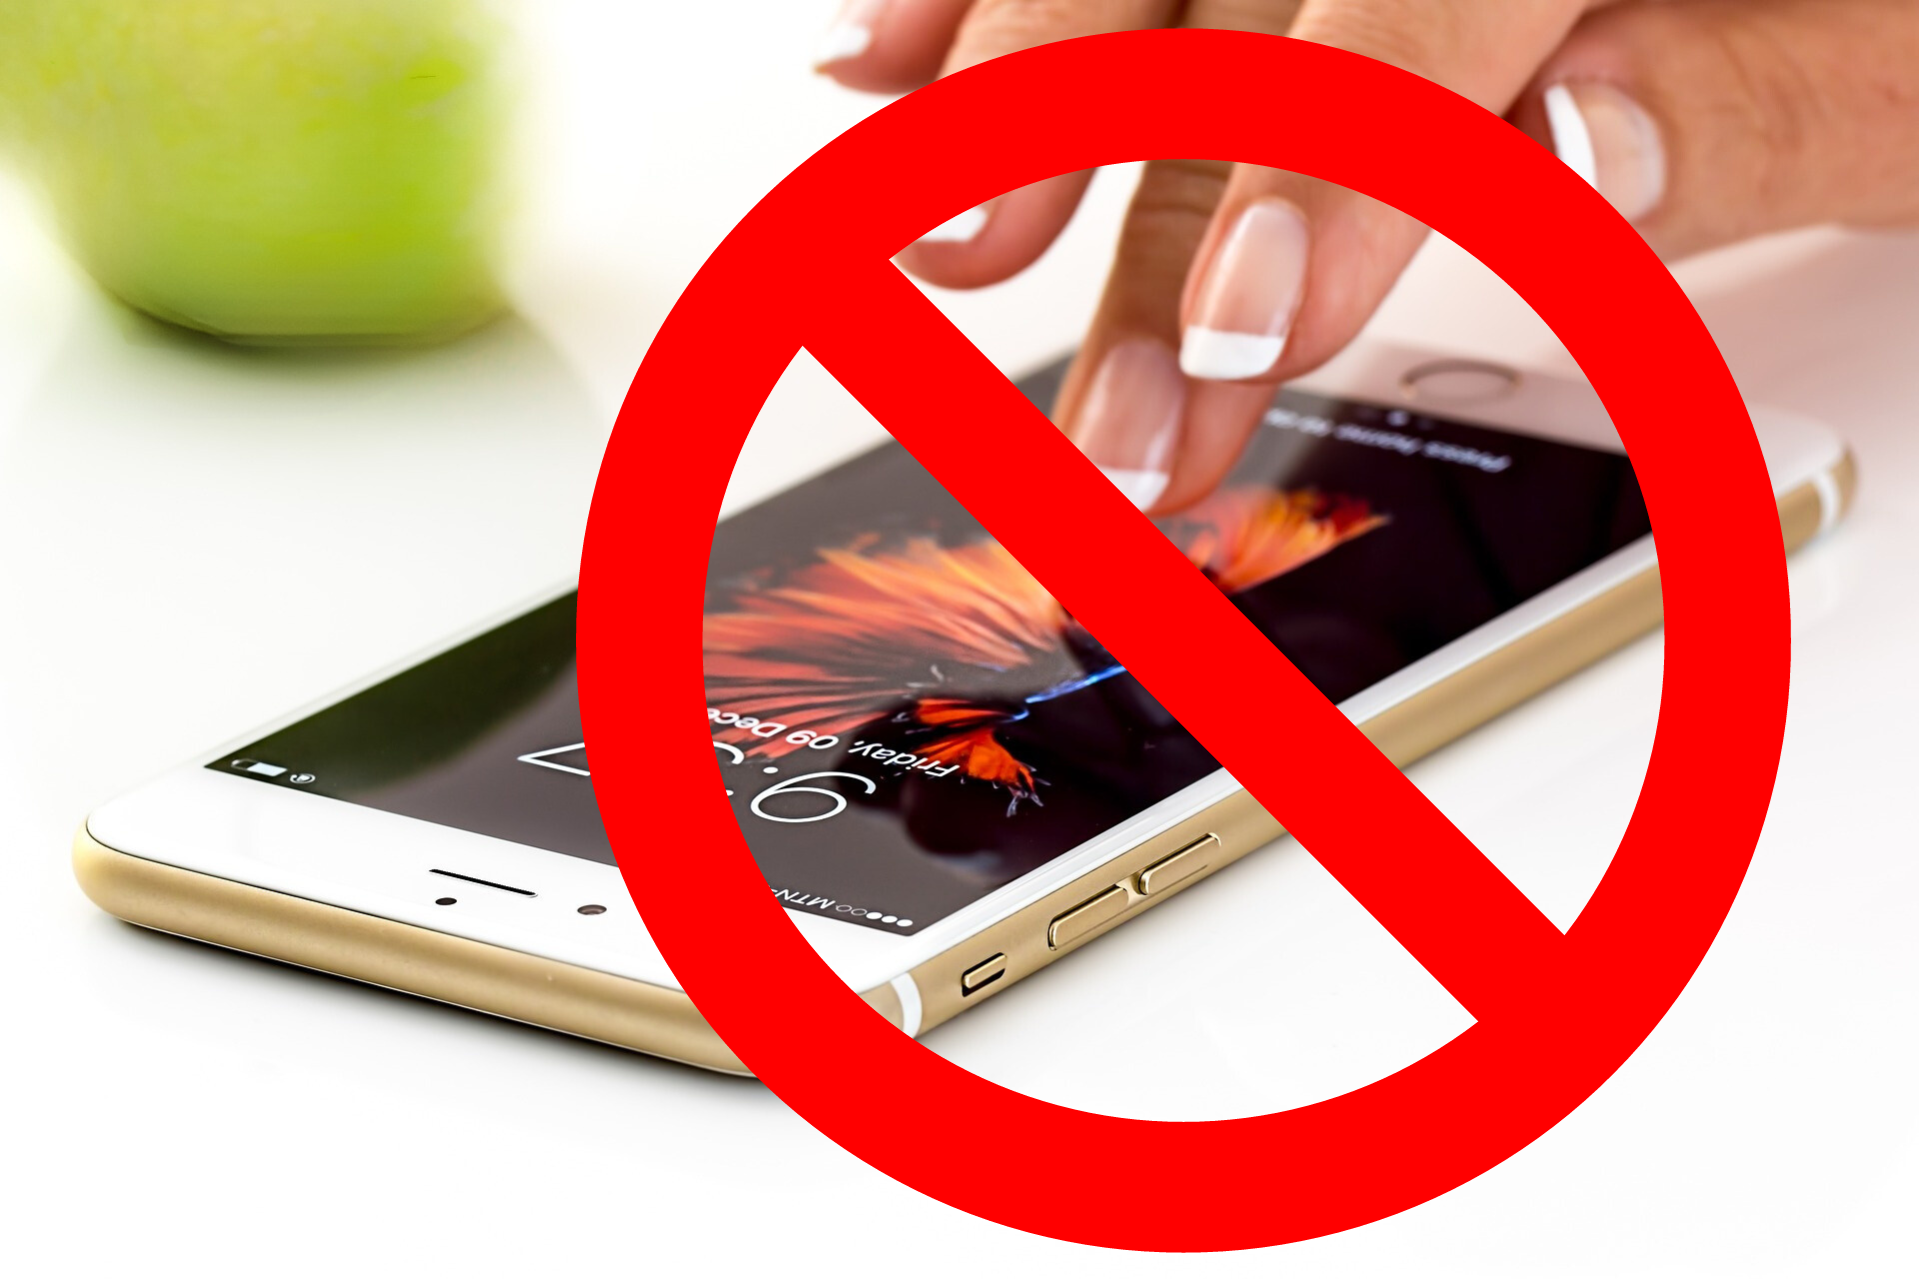
\includegraphics[width=2.21154in,height=1.55185in]{media/image39.png}

Redução: é o processo que realizamos quando queremos diminuir algo (como figuras planas, por exemplo) sem que suas características essenciais
sejam alteradas.

A figura representada teve seus lados divididos pela metade e manteve as mesmas
características. Observe.

%Fazer a figura a seguir sem marcar os ângulos e a primeira deve ter lado 6 cm e a segunda lado 3 cm.
%
\includegraphics[width=2.44231in,height=1.44820in]{media/image40.png}

Muitas vezes recorremos ao auxílio de malhas quadriculadas para nos
ajudar nesse processo.}

\colorsec{Atividades}

\num{1} Renato, aos finais de semana, anda de bicicleta ao redor da praça
que fica no bairro em que mora.

%Construir uma figura como essa nos padrões do projeto.
%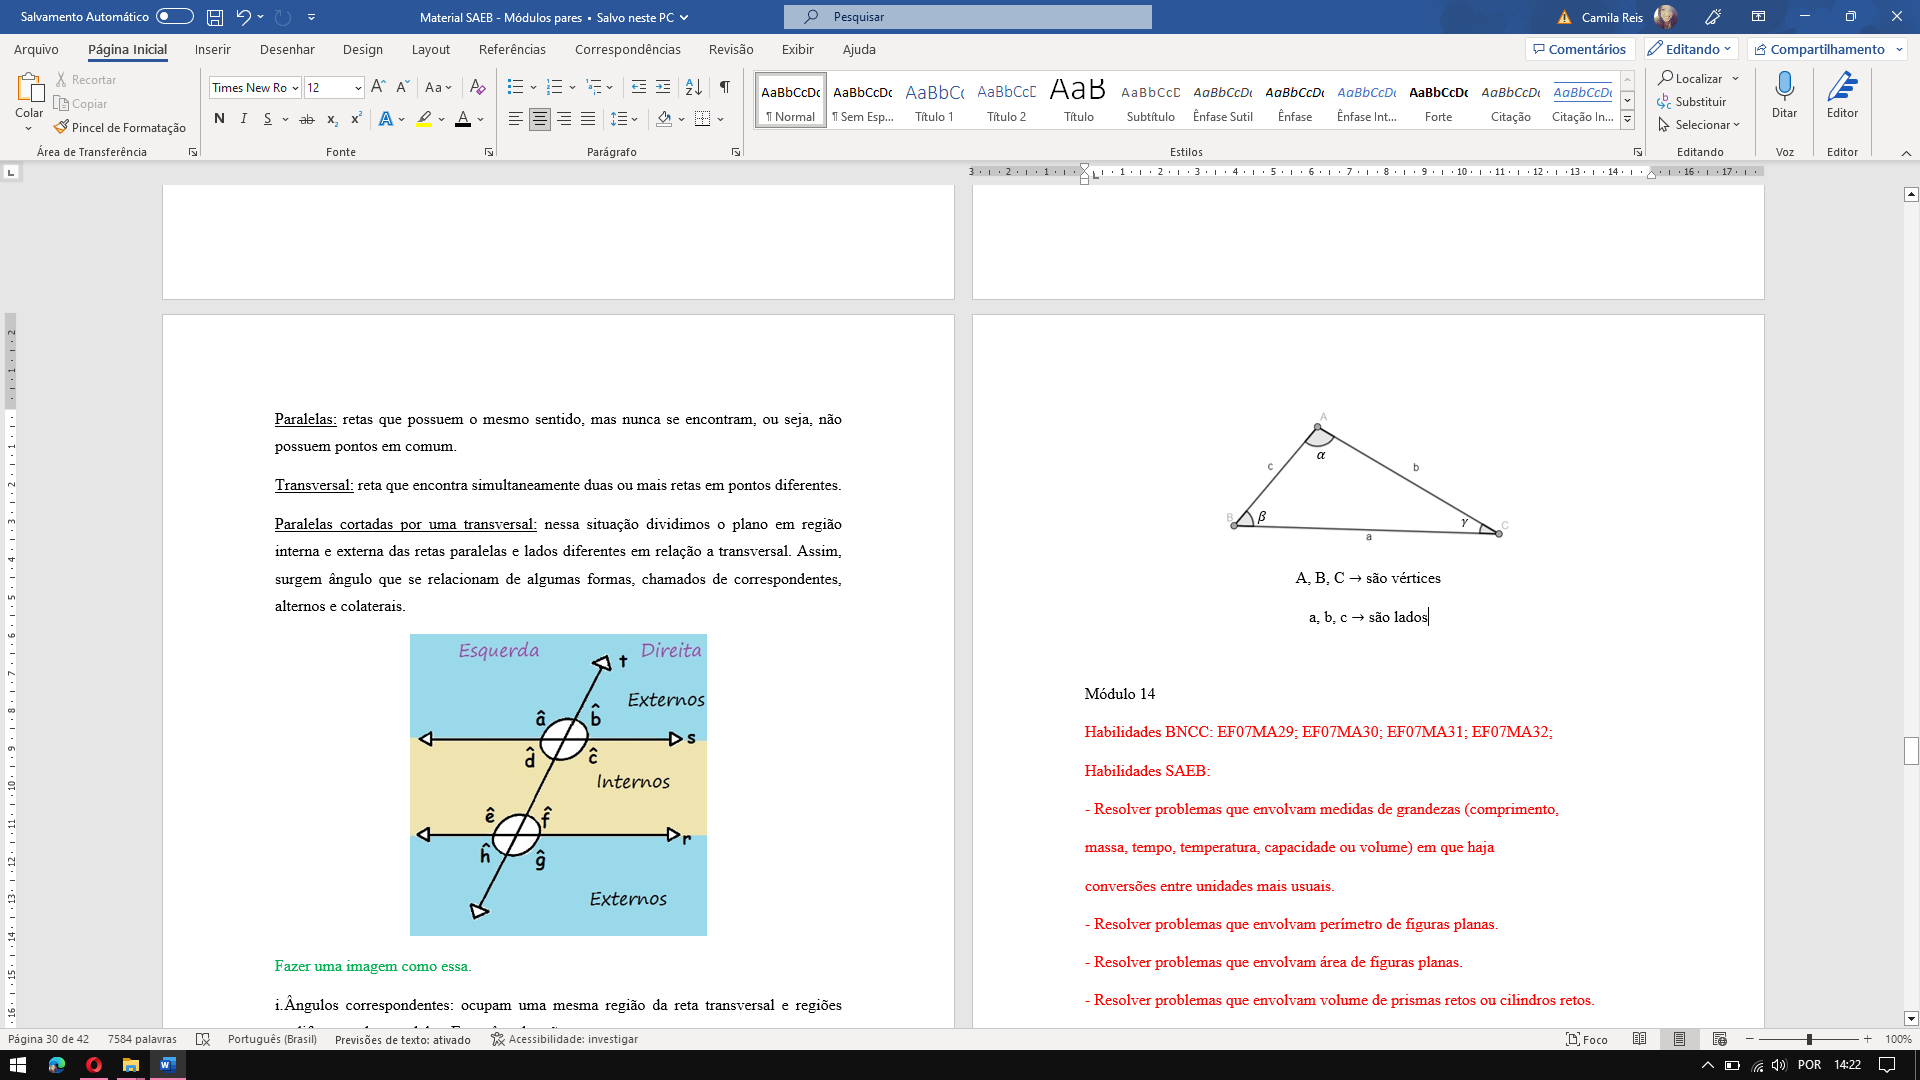
\includegraphics[width=2.35256in,height=2.20730in]{media/image41.png}

Se ele der duas voltas completas ao redor da praça, ele percorrerá qual
distância?

\matlinhas{2}

\coment{(2 x 30 + 2 x 50) x 2 = 320 m

Professor, sempre que possível, estimule a montagem da expressão para que
os alunos comecem a se acostumar.}

\num{2} Em uma atividade escolar a professora Helena forneceu uma figura e
seus alunos Ana, Rosa, Bernardo e Daiane deveriam realizar uma ampliação. Após algum tempo, os alunos entregaram seus desenhos.

%
\includegraphics[width=4.00833in,height=1.98932in]{media/image42.png}
% Construir uma figura conforme a anterior de acordo com os padrões do projeto.
% Colocar no lugar de Célia e Diana, os nomes Rosa e Daiane respectivamente.

Quem ampliou corretamente a imagem foi

\begin{escolha}
\item
  Ana.
\item
  Rosa.
\item
  Bernardo.
\item
  Daiane.
\end{escolha}

\coment{Resposta: Daiane, pois foi a única que manteve a proporcionalidade durante o
processo de ampliação.

Professor, devemos reforçar e discutir com os alunos os conceitos e
regras de ampliação e de redução.}

\num{3} Leandro resolveu cobrir de azuleijos o fundo de sua piscina, de tal
forma que apareça, nesse fundo, a letra inicial do nome de seu filho,
Arnaldo. Sabendo-se que cada quadradinho corresponde a um azuleijo,
quantos azuleijos foram utilizados para cobrir a letra inicial do nome
de seu filho?

%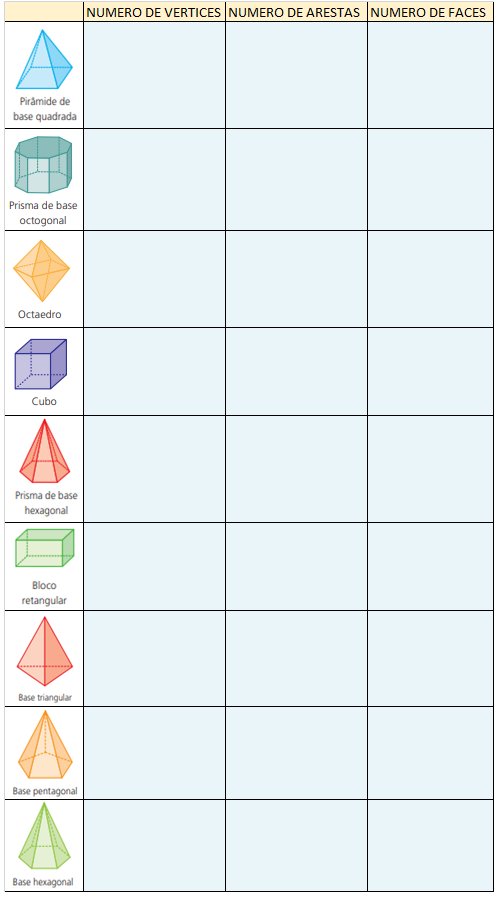
\includegraphics[width=1.42949in,height=1.25160in]{media/image43.png}
%Construir uma figura conforme a anterior de acordo com os padrões do projeto.


\coment{Resposta: 14.
Realizando a contagem do número de quadradinhos que formam a letra A,
percebemos que são 14 quadradinhos.}

\num{4} A entrada de um edifício está sendo reformada de tal forma que se
criem duas hortas comunitárias nas laterais; o restante do piso será coberto por um revestimento ecológico que permite a entrada da água da chuva no solo. Veja
a figura:

%
\includegraphics[width=2.49359in,height=1.70763in]{media/image44.png}
%Construir uma figura conforme a anterior de acordo com os padrões do projeto.

Estime a área que será destinada às duas hortas comunitárias.

\matlinhas{3}

\coment{
Podemos efetuar o cálculo correto de área: 2 x [(1 x 3)/2] = 3 metros
quadrados.
Mas, como o exercício pede para estimar, pode-se simplesmente
contar o número de quadradinhos que as áreas destinadas às hortas
ocuparão.

Professor, devemos estimular os dois cálculos, principalmente o segundo,
pois foge um pouco das formas tradicionais de cálculo e aguça percepção.

\num{5} Os desenhos representam os formatos, inicial  final, de uma praça que será construída em uma
área central de uma cidade. Inicialmente a previsão era de uma praça
pequena, mas, como a prefeitura conseguiu uma área maior ao lado da
primeira, optou-se por realizar a construção de uma praça maior.

%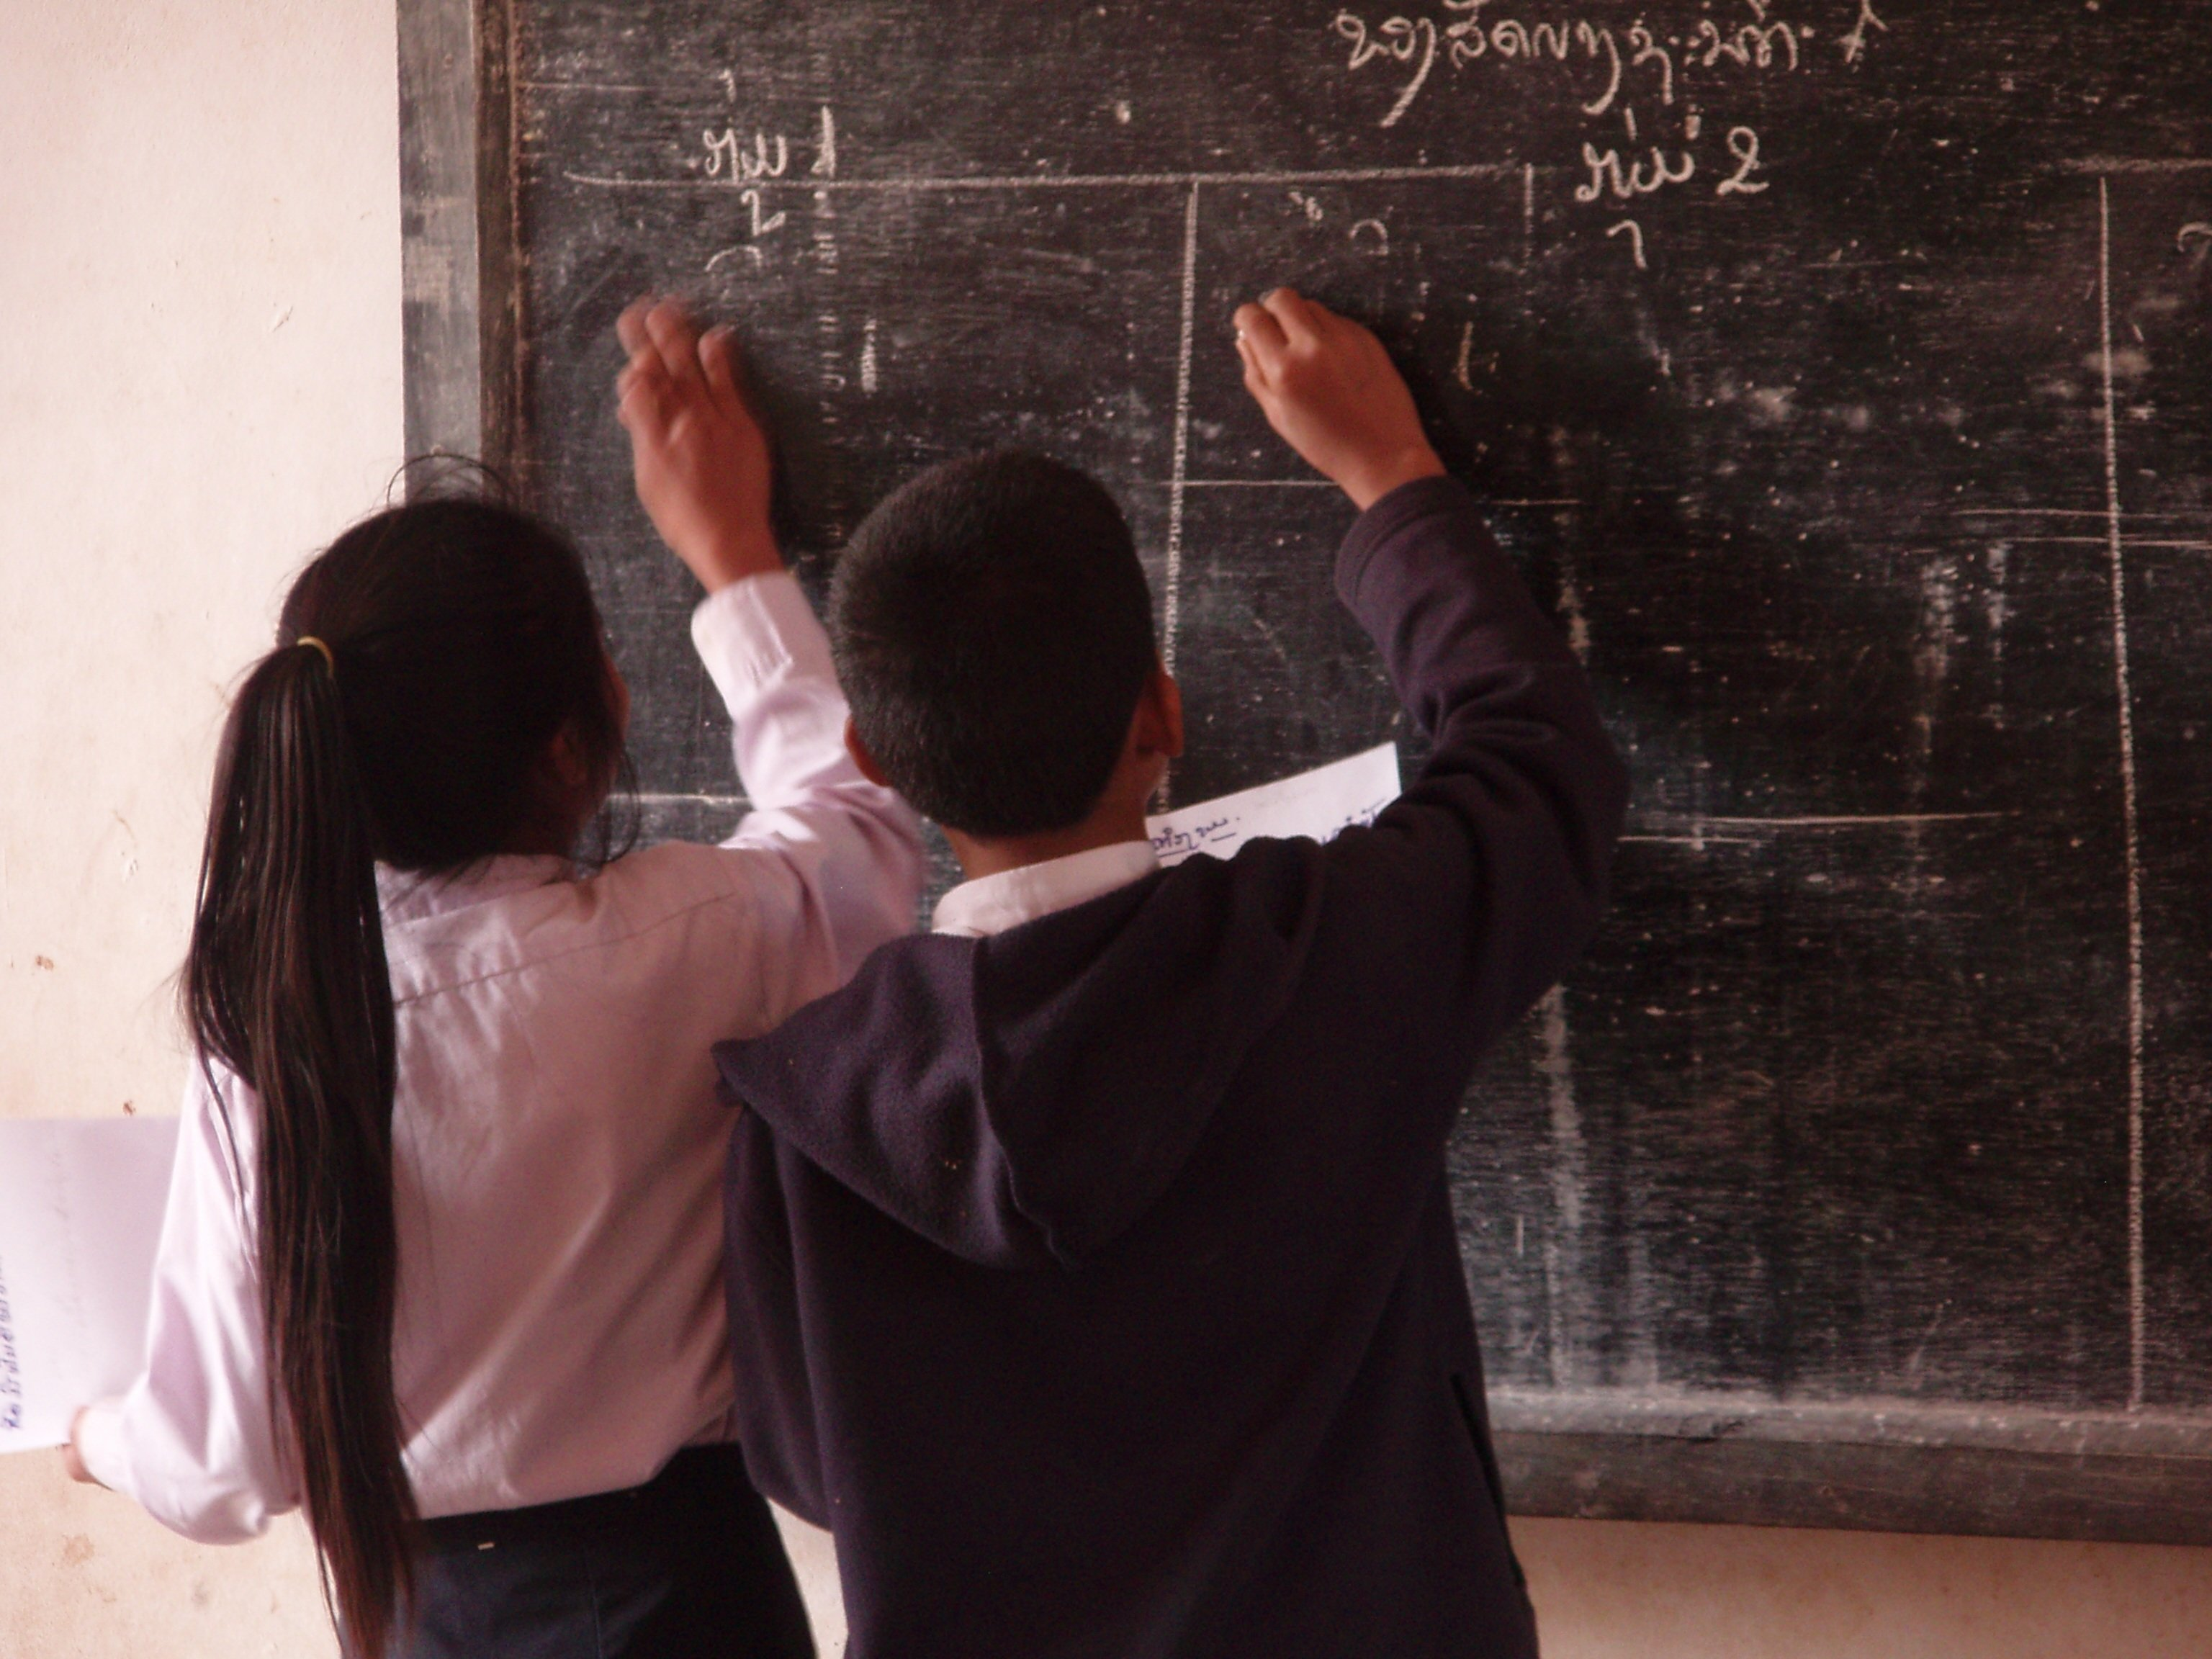
\includegraphics[width=5.00877in,height=1.80849in]{media/image45.png}
%Construir uma figura conforme a anterior de acordo com os padrões do projeto.

Sendo assim, a nova praça terá, com relação à praça que se
desejava construir iniciamente, uma área

\begin{escolha}
\item
  2 vezes maior.
\item
  3 vezes maior.
\item
  4 vezes maior.
\item
  5 vezes maior.
\end{escolha}

\coment{Resposta: C.
A praça menor teria 6 quadradinhos preenchendo sua área, enquanto a
grande terá 24 quadradinhos; sendo assim, a área da praça maior é
quatro vezes a área da praça menor.}

\num{6} Observando atentamente as figuras, pode-se perceber que a figura com a menor área é:

%
\includegraphics[width=5.12179in,height=1.48342in]{media/image46.png}
%Construir uma figura conforme a anterior de acordo com os padrões do projeto.


\coment{
A figura 2, composta por 4 quadradinhos.

A figura 1 é composta por 6 quadradinhos.
A figura 3 é composta por 5 quadradinhos.
A figura 4 é composta por 7 quadradinhos.

Como os quadradinhos são de mesmo tamanho, pode-se concluir que a figura
que possui a menor área é a figura 2, por ser composta por um número
menor de quadradinhos.

Professor, explore bastante esse conceito de percepção por meio da divisão
em pedaços menores de mesma medida, estimulando o senso de
comparação.}

\num{7} Um arquiteto fez um primeiro esboço de uma construção no formato de
cruz que teria que executar.

%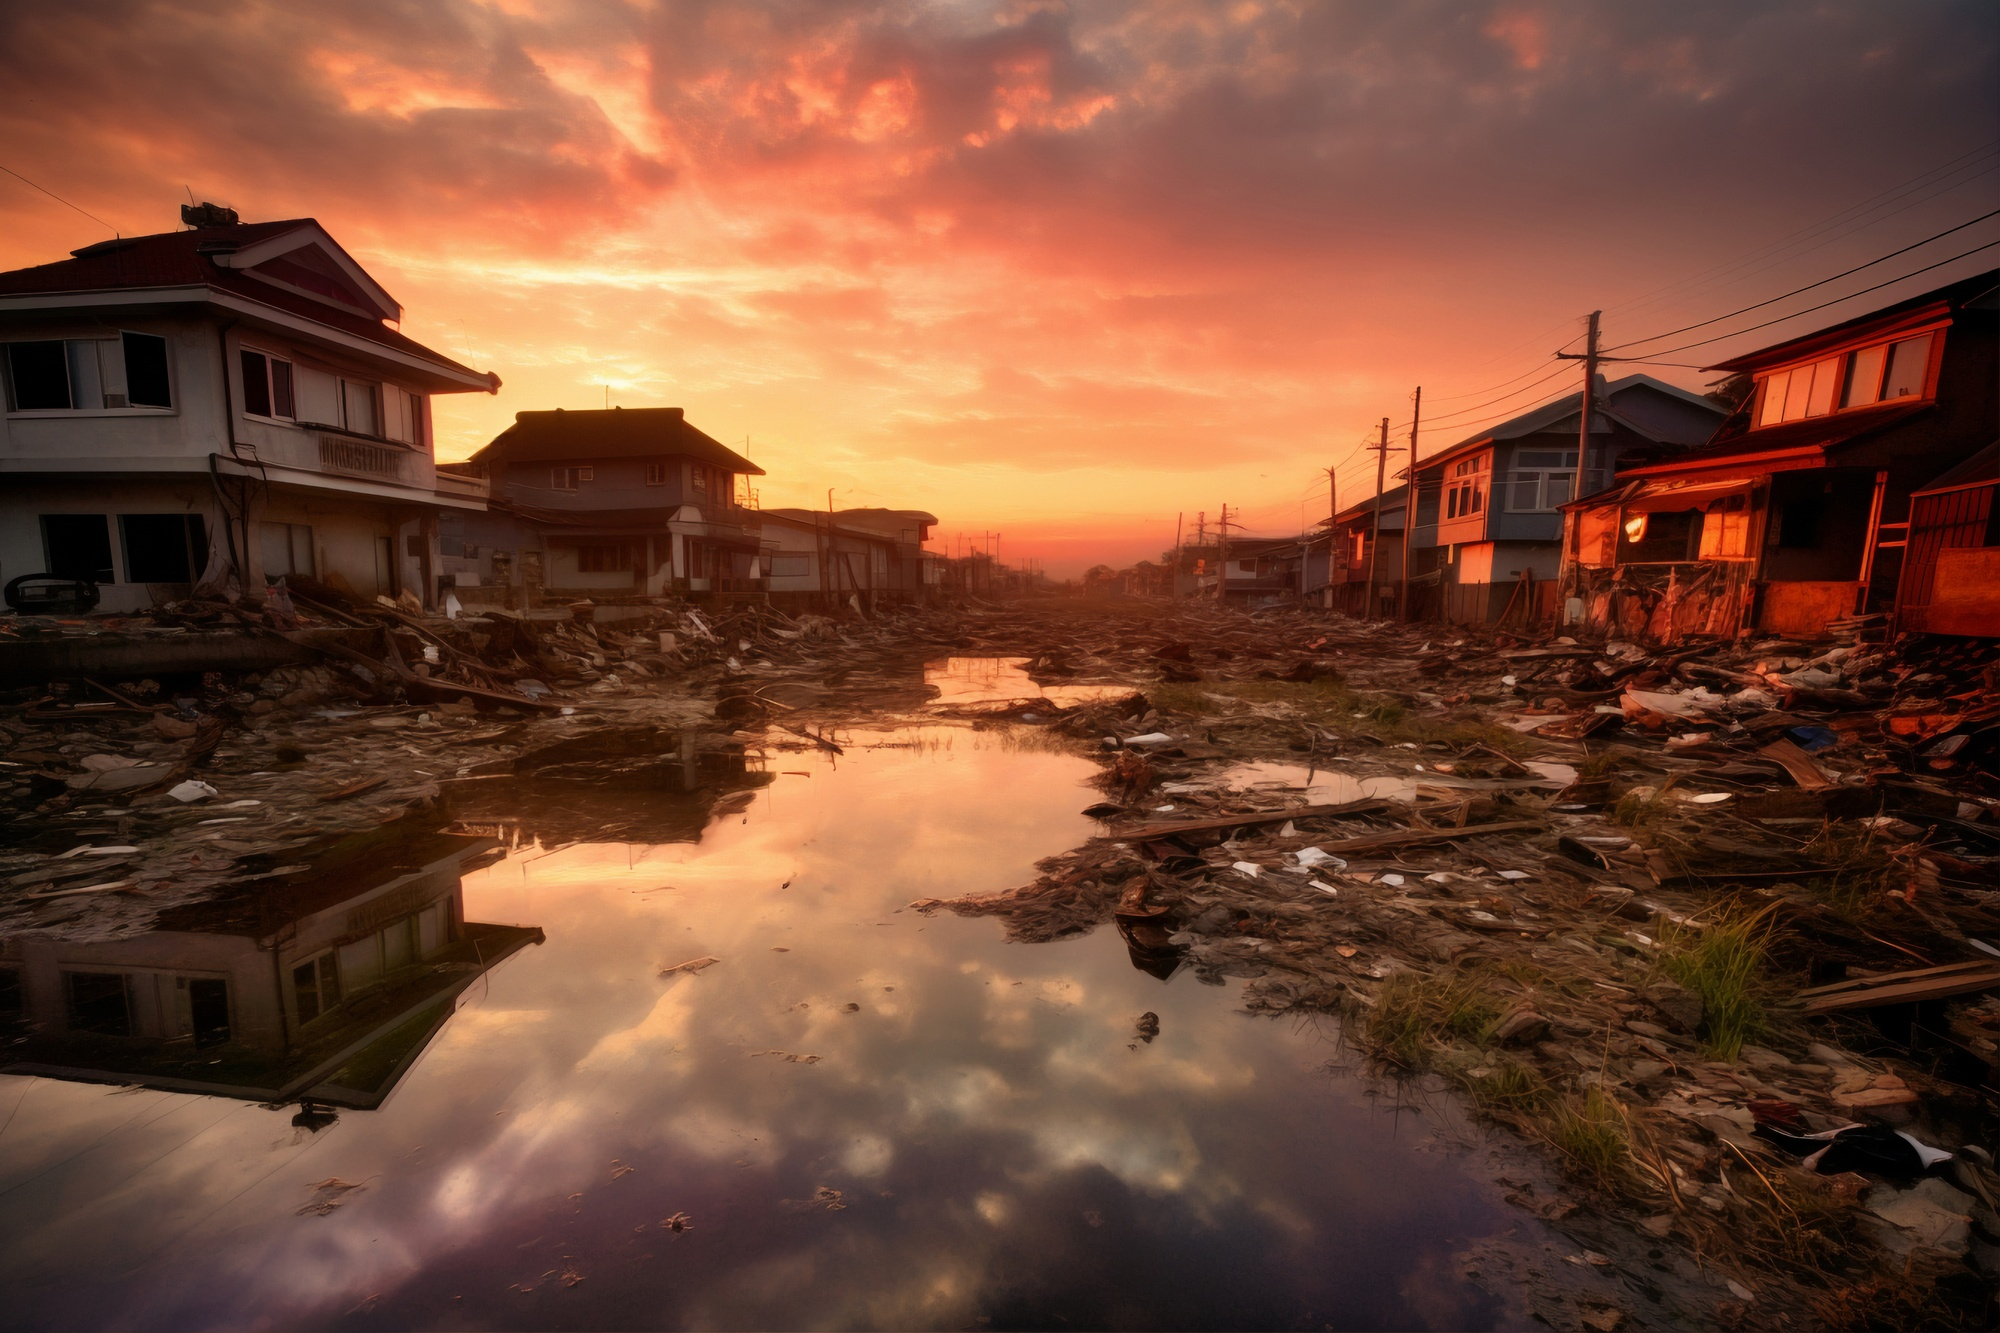
\includegraphics[width=2.27520in,height=1.51680in]{media/image47.png}
%Construir uma figura conforme a anterior de acordo com os padrões do projeto.

Mas, no projeto final, todos os lados foram reduzidos à metade. Qual das
figuras a seguir representa a nova construção em cruz?

%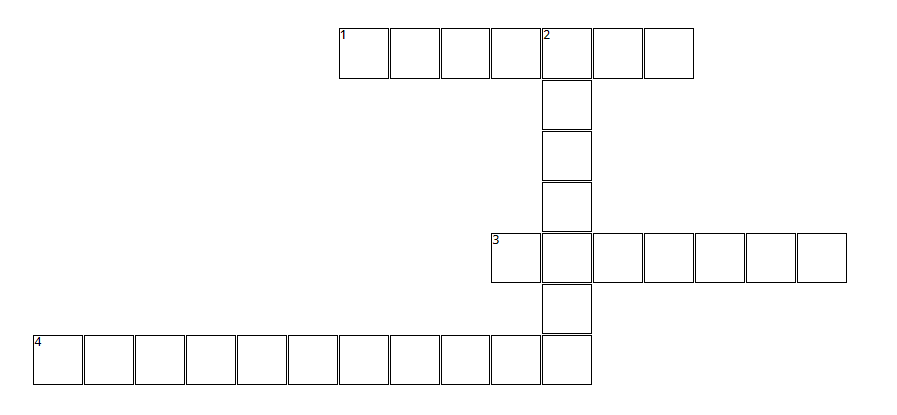
\includegraphics[width=5.90556in,height=1.42639in]{media/image48.png}
%Construir uma figura conforme a anterior de acordo com os padrões do projeto.

\coment{Figura A.
Reduzindo todos os lados pela metade e mantendo-se a proporção, conclui-se
que a figura correta é a representada na alternativa A.}

\num{8} Na malha quadriculada, cada quadrado representa uma área de
20 metros quadrados.

%\includegraphics[width=3.33333in,height=1.50517in]{media/image49.png}
%Construir uma figura conforme a anterior de acordo com os padrões do projeto.

Qual área da malha quadriculada a figura destacada ocupa?

\linhas{2}

\coment{
Realizando a contagem de quadradinhos que preenchem a figura, chega-se à conclusão de que,
que para o preenchimento dela, são necessários 16 quadradinhos.

Portanto, 16 x 20 = 320 metros quadrados.}

\num{9} Gabriel achou nas coisas guardadas de seu irmão mais velho a
seguinte malha quadriculada com letras destacadas:

%\includegraphics[width=4.36538in,height=1.60417in]{media/image50.png}
%Construir uma figura conforme a anterior de acordo com os padrões do projeto.

Dentre elas existem duas que ocupam superfícies de mesmo tamanho, que são

  A e E


\coment{Resposta: A e E.
Letra A: 14 quadradinhos.
Letra C: 11 quadradinhos.
Letra D: 13 quadradinhos.
Letra E: 14 quadradinhos.
Portanto, as duas letras que o cumpam asuperfícies de mesmo tamanho são A
e E.}

\num{10} Observe o terreno que Raimunda comprou representado em uma malha
quadriculada.

%\includegraphics[width=2.85256in,height=1.83420in]{media/image51.png}
%Construir uma figura conforme a anterior de acordo com os padrões do projeto.

Considerando que o lado de cada quadradinho representa 1 unidade de
medida de comprimento, o que deve acontecer com a medida de cada lado
para que o perímetro do terreno se reduza à metade, já que Raimunda quer
dar de presente para seu filho metade do terreno e ficar com a outra
parte?

\coment{Cada lado deve ser dividido por 2.
Para que o perímetro se reduza à metade, cada lado deve ser dividido por 2.}

\colorsec{Treino}

\num{1} Paulo resolveu ir a uma exposição e, no momento, está na bilheteria. Quanto ele precisará andar para chegar à exposição,
considerando o caminho destacado, sabendo-se que o lado de cada quadradinho da malha tem medida de 2m?

%\includegraphics[width=2.60897in,height=1.46587in]{media/image52.png}
%Construir uma figura conforme a anterior de acordo com os padrões do projeto.

\begin{escolha}
\item
  8 m.
\item
  10 m.
\item
  12 m.
\item
  14 m.
\end{escolha}

\coment{SAEB: Medir ou comparar perímetro ou área de figuras planas desenhadas em malha quadriculada.
Não há correspondência com a BNCC do quinto ano.

a) Incorreta. Nesse caso, seriam 4 lados de quadrado.
b) Correta. Ele deverá andar 5 lados de quadrado. Como cada lado de quadrado possui
medida igual a 2 m, ele deverá andar 10 metros.
c) Incorreta. Nesse caso, seriam 6 lados de quadrado.
d) Incorreta. Nesse caso, seriam 7 lados de quadrado.}

\num{2} O triângulo representado na malha quadriculada terá seus lados ampliados em duas vezes.

%\includegraphics[width=1.84615in,height=2.86967in]{media/image53.png}
%Construir uma figura conforme a anterior de acordo com os padrões do projeto.

As dimensões (lados) do novo triângulo terão que ser

\begin{escolha}
\item
  multiplicadas por 2.
\item
  divididas por 2.
\item
  subtraídas em duas unidades.
\item
  divididas por 4.
\end{escolha}

\coment{SAEB: Medir ou comparar perímetro ou área de figuras planas desenhadas em malha quadriculada.
Não há correspondência com a BNCC do quinto ano.

a) Correta. Como cada lado será ampliado em duas vezes, as medidas dos lados do novo
triângulo deverão ser dobradas, ou seja, multiplicadas por 2.
b) Incorreta. Nesse caso, o triângulo seria reduzido.
c) Incorreta. Nese caso, o triângulo sofreria diminuição.
d) Incorreta. Nesse caso, a redução no tamanho do triângulo seria muito significativa.}

\num{3} Maria começou a se arrumar para um passeio com suas amigas na hora
em que o relógio estava marcando as horas da forma que aparece a seguir.

%\includegraphics[width=1.29487in,height=1.32633in]{media/image54.png}
%Construir uma figura conforme a anterior de acordo com os padrões do projeto.

Sabendo-se que ela terminou de se arrumar em 35 minutos, qual o horário
que o relógio estava marcando quando ela terminou de se arrumar?

\begin{escolha}
\item
  11 horas e 50 minutos.
\item
  12 horas.
\item
  12 horas e 5 minutos.
\item
  12 horas e 10 minutos.
\end{escolha}

\coment{SAEB: Identificar horas em relógios analógicos ou associar horas em relógios analógicos e digitais.
Não há correspondência com a BNCC do quinto ano.

a) Incorreta. Nesse caso, ela teria gastado apenas 15 minutos para se arrumar.
b) Incorreta. Nesse caso, ela teria gastado 25 minutos para se arrumar.
c) Incorreta. Nesse caso, Maria teria se arrumado em 30 minutos.
d) Correta. O relógio está marcando 11 horas e 35 minutos; se acrescentarmos a esse
horário 35 minutos, teremos no relógio 12 horas e 10 minutos.}

\chapter{6. Nosso dinheiro}

\colorsec{Habilidades do SAEB}

\begin{itemize}
\item Relacionar valores de moedas e/ou cédulas do sistema monetário
brasileiro, com base nas imagens desses objetos.

\item Resolver problemas que envolvam moedas e/ou cédulas do sistema
monetário brasileiro.
\end{itemize}

\conteudo{Professor, talvez este módulo esteja entre os mais essenciais no estudo da matemática do quinto ano. É muito
importante que os alunos comecem a entender como lidar com o dinheiro.
Explore ao máximo as atividades, além de outras situações que podem
despertar o interesse e promover um início da educação e da conscientização
financeira.

Conhecendo nosso dinheiro

%\includegraphics[width=1.80833in,height=1.75637in]{media/image55.png}Moeda
%de 5 centavos: R\$ 0,05
%https://img.freepik.com/fotos-gratis/dinheiro-moedas-brasileiras-5-centavos_58702-6209.jpg?w=1060\&%t=st=1677437125~exp=1677437725~hmac=c640dd9c5a2963fb4f314f44e074b714cda9416e178bd281b3d494e8262ac50e
%
%\includegraphics[width=1.50833in,height=1.45668in]{media/image56.png}Moeda
%de 10 centavos: R\$ 0,10
%
%\includegraphics[width=1.52500in,height=1.24749in]{media/image57.png}Moeda
%de 25 centavos: R\$ 0,25
%https://img.freepik.com/fotos-gratis/dinheiro-moedas-brasileiras-25-centavos_58702-6230.jpg?w=1060\&%t=st=1677437194~exp=1677437794~hmac=db98c5063a731e98b23627749d52c094bab4a2f113240f1f248ee1be7074b235
%
%\includegraphics[width=1.56667in,height=1.61849in]{media/image58.png}Moeda
%de 50 centavos: R\$ 0,50
%https://img.freepik.com/fotos-gratis/dinheiro-moedas-brasileiras-50-centavos_58702-6291.jpg?w=1060\&%t=st=1677437366~exp=1677437966~hmac=a914e13013ee69679658ce52473a57d18d6d23ed6356e75e5d5a34316e88cd82
%
%\includegraphics[width=2.11667in,height=2.01180in]{media/image59.png}Moeda
%de 1 real: R\$ 1,00.
%https://img.freepik.com/fotos-gratis/dinheiro-moedas-brasileiras-1-real_58702-6210.jpg?w=1060\&%t=st=1677437258~exp=1677437858~hmac=3314b729d5619da0bffa3b7ce7fe354ae155c324f94ca82e2cb356693ffc25dc
%
%\includegraphics[width=2.71068in,height=1.97500in]{media/image60.png}Ao
%lado de cada nota colocar: Nota de 2 reais: R\$ 2,00; Nota de 5 reais
%R\$ 5,00; Nota de 10 reais: R\$ 10,00; Nota de 20 reais: R\$ 20,00. Nota
%de 50 reais: R\$ 50,00
%https://img.freepik.com/vetores-gratis/ilustracao-gradiente-de-caixa-brasileira_52683-78831.jpg?w=996\&%t=st=1677437712~exp=1677438312~hmac=c23ec28122c2591b7b261ceca09eb7c0a64059387f9729dc642986ca98524f1c
%n
%
%\includegraphics[width=3.18285in,height=1.50833in]{media/image61.png}Nota
%de 100 reais R\$ 100,00
%
%https://img.freepik.com/fotos-premium/cem-reais-contas-dinheiro-brasileiro_499484-1535.jpg?w=1060
%
%\includegraphics[width=2.68333in,height=1.88913in]{media/image62.png}Nota
%de 200 reais: R\$ 200,00
}

\colorsec{Atividades}

\num{1} Marta foi à papelaria comprar uma caneta de que estava precisando para continuar seus estudos. Ela comprou uma caneta que custava 7 reais e 25
centavos. Sabendo-se que ela pagou com uma nota de 10 reais, quais
cédulas e moedas ela recebeu de troco?

\linhas{2}

\coment{Como o enunciado esclarece que são cédulas e moedas, ela deve ter recebido de troco uma nota de 2 reais, 1 moeda de 50 centavos e uma moeda de 25
centavos.

Existem outras opções; explore as outras combinações com seus alunos.

Professor, explore com os alunos outras situações para que treinem um pouco esse conceito. Além disso, converse um pouco com os alunos sobre
outras moedas que existem no mundo e sobre qual o seu valor em relação ao real e vice-versa.}

\num{2} Caíque economizou muito dinheiro, pois queria comprar um videogame
usado que custava R\$ 2.490,00 à vista. Ele conversou com o vendedor, pediu um desconto extra e foi atendido com um desconto de R\$ 250,00.
Quanto ele pagou pelo videogame?

\matlinhas{3}

\coment{R\$ 2.490,00 -- R\$ 250,00 = R\$ 2.240,00}

\num{3} A contadora de uma empresa está conferindo o saldo da conta
bancária e está desconfiado de que existe erro, pois o valor não bate com
os lançados em sua planilha.

%\includegraphics[width=3.32591in,height=1.58974in]{media/image63.png}
%Os valores devem ser colocados em um papel que imite um extrato bancário. Para facilitar como os números estão meio apagados, coloquei eles abaixo.

Saldo anterior: R\$12.350,34

Transferência depósito R\$ 1.230,90

Saque R\$ 350,00

Compra débito: R\$ 231,05

Ajude a contadora, descobrindo qual o erro que há no extrato da conta para, assim, saber o saldo correto.

\matlinhas{3}

\coment{
O saldo anterior era de R\$ 12.350,34 e, logo em seguida, tivemos um
depósito de R\$ 1.230,90, ficando o saldo igual a R\$ 13.581,24. Logo após, tivemos um saque de R\$ 350,00 e uma compra em débito de R\$ 231,05. Isso deixou o saldo igual a R\$ 13.000,19.}

\num{4} Em muitas compras a prazo é exigida uma entrada, que é paga no ato
da compra. O restante do valor pode ser dividido em um número combinado
de parcelas mensais. Veja o exemplo.

%Construir uma imagem conforme a abaixo
%\includegraphics[width=2.90025in,height=0.89174in]{media/image64.png}

%O escrito deve ser: 

Entrada de R\$ 25.000,00 e o restante dividido em 24
parcelas de R\$ 1.500,00 cada uma.

\begin{escolha}
\item
  Qual o valor que será dividido em 24 vezes?

\matlinhas{3}

\item
  Qual o valor que cada parcela terá?

\matlinhas{3}

\item
  Se à vista a loja fornece um desconto de R\$ 2. 580,00, quem optar por
  pagar à vista pagará quanto pela mercadoria?

\matlinhas{3}
\end{escolha}

\coment{
a) 24 x 1.500,00 = R\$ 36 000,00.
b) Lendo atentamente o texto, sabe-se que será de R\$ 1 500,00.
c) 25.000,00 + (24 x 1.500,00) -- 2.580,00 = R\$ 58 420,00.

Professor, incentive os alunos a fazer a montagem da expressão, mesmo que
encontrem outra saída de resolução. Não devemos inibir outras resoluções, mas sim mostrar várias formas e, dentre elas, a montagem da expressão.}

\num{5} Complete os quadros com as quantidades de cada nota para que se obtenham os valores estipulados.

%\begin{enumerate}
%\def\labelenumi{\alph{enumi})}
%\item
%\end{enumerate}
%
%\includegraphics[width=4.14203in,height=1.14177in]{media/image65.png}
%
%Construir a imagem acima. No lugar de R\$ 836,00 colocar R\$ 966,00
%
%\begin{enumerate}
%\def\labelenumi{\alph{enumi})}
%\item
%\end{enumerate}
%
%\includegraphics[width=4.10036in,height=1.20844in]{media/image66.png}
%
%Construir a imagem acima. Deixar só o valor R\$ 3 940,00 e deletar o de
%R\$ 1 700,00

\coment{
Professor, podem surgir outras combinações para a resposta. Incentive e estimule essa criatividade.

a) Uma possibilidade para R\$ 966,00 podem ser 48 notas de 20 reais e 3 notas de 2 reais.
b) Uma possibilidade para R\$ 3.940,00 podem ser 15 notas de 200 reais, 9 notas de 100 reais e 2 notas 20 reais.}

\num{6} Complete a tabela, levando em conta o valor real de cada
moeda, conforme o que aparece na primeira linha como exemplo.

%Construir a imagem abaixo atento a quantidade pois são importantes na
%resolução.
%
%\includegraphics[width=2.82051in,height=3.34367in]{media/image67.png}


Mariana está pesquisando em um site de compras on-line o preço de
algumas coisas de que está precisando.

%Construir a imagem abaixo nos moldes do projeto:
%
%\includegraphics[width=3.75866in,height=1.47513in]{media/image68.png}

\num{7} 
  Qual a menor quantidade de moedas de 1 real de que ela precisará para
  pagar 2 unidades de cada item, caso decida comprar?

\matlinhas{3}

\num{8} 
  Qual o troco que ela deverá receber?
\end{escolha}

\matlinhas{2}

\coment{
Preço a pagar: 2 x (0,80 + 0,50 + 0,95 + 0,35) = R\$ 5,20. apara esse
valor ela precisará de 6 moedas de 1 real e terá R\$ 0,80 de troco.}

\num{9} Observe atentamente a propaganda de determinado supermercado.

%Construir a imagem abaixo nos moldes do projeto:
%\includegraphics[width=4.00868in,height=1.94184in]{media/image69.png}

\begin{enumerate}
\item
  Escreva como deve ser lido o preço de cada um dos produtos anunciados.

\linhas{5}

\item
  Construa uma sequência decrescente com os preços dos produtos anunciados.

\linhas{1}

\item
  Quantas notas de 20 reais são necessárias para adquirir uma unidade de
  cada produto anunciado?

\matlinhas{3}

\item
  Qual o troco que essa pessoa receberá se pagar conforme a situação anterior?

\matlinhas{3}
\end{enumerate}

\coment{
a)  R\$ 3,75: três reais e setenta e cinco centavos.
R\$ 7,30: sete reais e trinta centavos.
R\$ 3,25: três reais e vinte e cinco centavos.
R\$ 3,99: três reais e noventa e nove centavos.
R\$ 15,80: quinze reais e oitenta centavos;
b)  (15,80; 7,30; 3,99; 3,75; 3,25);
c) 3,75 + 7,30 + 3,25 + 3,99 + 15,80 = R\$ 34,09. Portanto, 2 notas de 20 reais são necessárias;
d)  40 -- 34,09 = R\$ 5,91.}

\num{10} Valentina vendeu algumas coisas que não utilizava mais e, como
pagamento, recebeu um cheque em que estava escrito: "doze mil quatrocentos
e cinquenta e nove reais". Como sua conta estava sem dinheiro algum, ela
resolveu depositar o cheque. No dia seguinte, realizou uma compra no cartão de débito no valor de R\$ 12.305,92. Após essa operação, qual o
saldo de Valentina em sua conta bancária?

\matlinhas{3}

\coment{R\$ 12.459,00 -- R\$ 12.305,92 = R\$ 153,08}

\colorsec{Treino}

\num{1} Maria Luísa resolveu trocar as moedas que ganhou de seu avô por
notas de 2 reais com seu primo, Francisco. Em seu cofre havia 12 moedas de 50 centavos e 8 moedas de 25 centavos. Quantas notas de 2
reais ela recebeu de seu primo nessa troca?

\begin{escolha}
\item
  4
\item
  6
\item
  8
\item
  20
\end{escolha}

\coment{SAEB: Resolver problemas que envolvam moedas e/ou cédulas do sistema monetário brasileiro.
Não há correspondência com a BNCC do quinto ano.

a) Correta.
12 x 0,50 + 8 x 0,25 = 6 + 2 = R\$ 8,00. Portanto, 4 notas de 2 reais.
b) Incorreta. 6 notas de 2 reais totalizariam R\$ 12,00.
c) Incorreta. 8 notas de 2 reais totalizariam R\$ 16,00.
d) Incorreta. 20 notas de 2 reais totalizariam R\$ 40,00.}

\num{2} Letícia resolveu arrumar as coisas que estavam em sua bolsa e
encontrou os seguintes valores:

%Construir a imagem abaixo nos moldes do projeto. \textbar{}Atento as quantidades pois fazem parte do exercício. \includegraphics[width=5.90556in,height=1.78681in]{media/image70.png}

Após uma contagem rápida, ela concluiu que possuía em sua bolsa a quantia de

\begin{escolha}
\item
  R\$ 9,00.
\item
  R\$ 9,90.
\item
  R\$ 10,10.
\item
  R\$ 10,15.
\end{escolha}

\coment{SAEB: Relacionar valores de moedas e/ou cédulas do sistema monetário brasileiro, com base nas imagens desses objetos.
Não há correspondência com a BNCC do quinto ano.

a) Incorreta. R\$ 9,00 é o valor somente das células.
b) Incorreta. R\$ 9,90 seria o valor das células mais R\$ 0,90 em moedas.
c) Incorreta. R\$ 10,10 seria um valor R\$ 0,05 menos que o total encontrado.
d) Correta. 
R\$ 9,00 em cédulas e R\$ 1,15 em moedas. Portanto, no total, ela
encontrou em sua bolsa R\$ 10,15.}

\num{3} Na lanchonete a que Augusto costuma ir com seus amigos, encontra-se a
seguinte tabela de preços:

\begin{longtable}[]{@{}ll@{}}
\toprule
Produtos & Valor por unidade\tabularnewline
\midrule
\endhead
Pão de queijo & R\$ 3,00\tabularnewline
Bombom & R\$ 5,00\tabularnewline
Suco & R\$ 6,00\tabularnewline
Doce & R\$ 4,50\tabularnewline
Refrigerante & R\$ 4,50\tabularnewline
Cachorro-quente & R\$ 12,00\tabularnewline
\bottomrule
\end{longtable}

Na última vez que Augusto foi a esse lugar, ele comprou 2 bombons, 1
suco e 1 cachorro-quente. Qual o valor gasto por Augusto nesse dia?

\begin{escolha}
\item
  R\$ 18,00.
\item
  R\$ 22,00.
\item
  R\$ 28,00.
\item
  R\$ 30,00.
\end{escolha}

\coment{SAEB: Resolver problemas que envolvam moedas e/ou cédulas do sistema monetário brasileiro.
Não há correspondência com a BNCC do quinto ano.

a) Incorreta. R\$ 18,00 seriam R\$ 10,00 a menos do que o valor pago.
b) Incorreta. R\$ 22,00 seriam R\$ 6,00 a menos do que o valor pago.
c) Correta. 2 x 5,00 + 1 x 6,00 + 1 x 12,00 = 10,00 + 6,00 + 12,00 = R\$ 28,00.
d) Incorreta. R\$ 30,00 seriam R\$ 2,00 a mais do que o valor pago.

Professor, você pode utilizar este exercício e estimular os alunos a
realizarem outras combinações conforme a preferência de cada um e
encontrarem qual o valor que eles pagariam nessa lanchonete pelo respectivo pedido.}

\chapter{7. Chances e possibilidades}

\coment{Habilidades da BNCC: EF05MA22, EF05MA23.}

\colorsec{Habilidades do SAEB}

\begin{itemize}
\item Identificar, entre eventos aleatórios, aqueles que têm menos, maiores ou
iguais chances de ocorrência, sem utilizar frações.

\item Determinar a probabilidade de ocorrência de um resultado em eventos
aleatórios, quando todos os resultados possíveis têm a mesma chance de
ocorrer (equiprováveis).
\end{itemize}

\conteudo{Probabilidade é um conceito extremamente importante
em provas futuras que os alunos farão. Explore ao máximo os conceitos com eles,
falando de uma maneira leve e interessante para que desperte o gosto da maioria.

PROBABILIDADE: é um número p, , que indica a chance de um determinado
resultado ocorrer. O número 0 representa uma probabilidade de 0\%, ou
seja, chance nenhuma de o resultado ocorrer; o número 1
corresponde à probabilidade do 100\%, o que quer dizer que certamente o evento ocorrerá.

FENÔMENOS ALEATÓRIOS: são fenômenos sobre os quais, mesmo com conhecimento de todos os
resultados possíveis, não podemos, a cada ocorrência, precisar o
resultado final.

ESPAÇO AMOSTRAL (E): é o conjunto que reúne todos os resultados
possíveis de um fenômeno aleatório.

EVENTO (A): é o conjunto que reúne todos os resultados de interesse.}

\colorsec{Atividades}

\num{1} Em um estojo há 25 lápis coloridos e 18 lápis pretos. Retirando-se, ao
acaso, um lápis desse estojo, qual é a maior chance: retirar um lápis
colorido ou um preto? Justifique sua resposta.

\matlinhas{3}

\coment{Como há mais lápis coloridos do que pretos no estojo, a maior chance
quando se retira um único lápis desse estojo é que saia um lápis
colorido.

Professor, aproveite este exercício para dar outros exemplos e, aos poucos,
ir trabalhando esse conceito em seus alunos devido à importância de eles
desenvolverem essa habilidade para encontrarem maiores chances através de uma
simples análise.}

\num{2} Daniel joga um dado honesto. Calcule a probabilidade de Daniel:

\begin{escolha}
\item
  Tirar, na face voltada para cima, um número par.

\matlinhas{2}

\item
  Tirar, na face voltada para cima, um número ímpar.

\matlinhas{2}

\item
  Tirar, na face voltada para cima, um número menor do que 3.

\matlinhas{2}
\end{escolha}

\coment{
a)  Temos 6 possibilidades de números que podem sair: 1, 2, 3, 4, 5 e 6.
Interessa um número par: 2, 4 e 6.
Portanto, a probabilidade será de 3/6 = ½ = 0,50 = 50\%.
b)  Temos 6 possibilidades de números que podem sair: 1, 2, 3, 4, 5 e 6.
Interessa um número ímpar: 1, 3 e 5.
Portanto, a probabilidade será de 3/6 = ½ = 0,50 = 50\%.
c)  Temos 6 possibilidades de números que podem sair: 1, 2, 3, 4, 5 e 6.
Interessa um número menor que 3: 1 e 2.
Portanto, a probabilidade será de 2/6 = 1/3.

Professor, deixe bem claro para os alunos que podemos representar o
resultado com uma fração, com um decimal ou com uma porcentagem.}

\num{3} Uma sacola escura, que não permite visualizar o que há dentro,
contém 20 bolas idênticas, mas de cores diferentes. Sabe-se que 6 são
azuis, 8 são pretas, 4 são vermelhas e 2 são amarelas. Retirando-se uma
bola ao acaso, calcule:

\begin{escolha}
\item
  A probabilidade de ela ser azul.

\matlinhas{2}

\item
  A probabilidade de a bola não ser da cor preta.

\matlinhas{2}.
\end{escolha}

\coment{
a) 6/20 = 3/10 = 0,30 = 30\%.
b) (6 + 4 + 2)/20 = 12/20 = 6/10 = 0,60 = 60\%.

Professor, comece a mostrar para o aluno os conceitos de probabilidade
complementar e deixe bem claro que a probabilidade máxima de algo
acontecer é 100\%, assim como a mínima é 0\%.}

\num{4} Lucas tem guardados em uma caixa 12 livros de matemática, 3 de
história e 5 de Geografia. Retirando-se um desses livros, ao acaso, da
caixa, calcule:

\begin{escolha}
\item
  A probabilidade de ele ser um livro de matemática.

\matlinhas{2}

\item
  A probabilidade de ele ser um livro de português.

\matlinhas{2}
\end{escolha}

\coment{
a) 12/(12 +3 + 5) = 12/20 = 6/10 = 0,60 = 60\%.
b) A probabilidade é de 0\%; ou seja, é impossível sair um livro de
  português, visto que na caixa não há livros dessa disciplina.}

\num{5} Na sala em que Clarissa estuda há 26 alunos, dos quais 18 são
meninas. A professora irá escolher um aluno para verificar se este fez a
tarefa. Qual a probabilidade de um menino ser escolhido?

\matlinhas{3}

\coment{
Total de alunos: 26.
Número de meninos: 26 -- 18 = 8.
Portanto, a probabilidade será de 8/26 = 4/13.}

\num{6} Uma letra é escolhida ao acaso dentre as que formam a palavra
FUNDAMENTAL. Qual a probabilidade de a letra escolhida ser uma vogal?

\matlinhas{3}

\coment{
Total de letras: 11.
Vogais: 4.
Portanto, a probabilidade pedida será de 4/11.}

\num{7} O baralho convencional é composto por 52 cartas divididas em quatro
naipes (copas, paus, ouros e espadas), sendo 13 de cada naipe. Dessa
forma, se retirarmos uma carta ao acaso, qual a probabilidade de sair
uma carta do naipe de copas?

\matlinhas{3}

\coment{
Total de cartas: 52.
Cartas de copas: 13.
Probabilidade = 13/52 = ¼ = 0,25 = 25\%.}

\num{8} Vítor quer escolher um número para sua camiseta do time de futebol
e ele pode escolher qualquer número de 1 a 16. Qual a probabilidade de
que ele escolha um número maior que 8 e menor que 14?

\matlinhas{3}

\coment{
Total de números: 16.
Total de números que interessam: 5.
Probabilidade = 5/16}

\num{9} Os 500 estudantes de um colégio responderam a uma pergunta sobre
qual a sua área de conhecimento preferida (entre Exatas, Humanidades e
Biológicas). As respostas foram computadas e alguns dados foram colocados
na tabela.

\begin{longtable}[]{@{}ll@{}}
\toprule
Área & Sexo\tabularnewline
& Masculino (M)\tabularnewline
Exatas (E) & 120\tabularnewline
Humanas (H) & 45\tabularnewline
Biológicas (B) & 100\tabularnewline
Total & 265\tabularnewline
\bottomrule
\end{longtable}

Um estudante é escolhido ao acaso. Determine a probabilidade de esse
estudante preferir Humanidades.

\matlinhas{3}.

\coment{
Total de estudantes: 500.
Preferência por Humanidades: 125.
Probabilidade: 125/500 = ¼ = 0,25 = 25\%.}

\num{10} Carlos tem duas urnas com bolas que só são diferenciadas pela
cor. A distribuição das bolas nas urnas e por cor se encontra na tabela
a seguir.

\begin{longtable}[]{@{}lll@{}}
\toprule
Cor & Urna 1 & Urna 2\tabularnewline
\midrule
\endhead
Amarela & 4 & 0\tabularnewline
Azul & 3 & 1\tabularnewline
Branca & 2 & 2\tabularnewline
Verde & 1 & 3\tabularnewline
Vermelha & 0 & 4\tabularnewline
\bottomrule
\end{longtable}

Carlos colocará todas as bolas dessas duas urnas em uma única urna 3. Em
seguida, retirará uma bola, ao acaso, dessa última urna. Qual a
probabilidade de que ele retire uma bola verde?

\matlinhas{3}

\coment{
Total de bolas: 20.
Bolas verdes: 4.
Probabilidade: 4/20 = 2/10 = 0,20 = 20\%}

\colorsec{Treino}

\num{1} Mateus precisa ir ao dentista nesta semana. Escolhendo ao acaso um
dia da semana para ir ao dentista, qual a probabilidade de Mateus
escolher uma segunda-feira ou uma quinta-feira?

\begin{escolha}
\item
  1/7
\item
  2/7
\item
  1/5
\item
  2/5
\end{escolha}

\coment{SAEB: Determinar a probabilidade de ocorrência de um resultado em eventos aleatórios, quando todos os resultados possíveis têm a mesma chance de ocorrer (equiprováveis).
BNCC: EF05MA23 -- Determinar a probabilidade de ocorrência de um resultado em eventos aleatórios,
quando todos os resultados possíveis têm a mesma chance de ocorrer (equiprováveis).

a) Incorreta. Nesse caso, trata-se da chance de escolha de apenas um dia da semana.
b) Correta. 
Dias da semana: 7.
Escolhas determinadas: 2.
Probabilidade: 2/7.
c) Incorreta. Essa seria a chance de uma escolha dentre 5 possibilidades.
d) Incorreta. Nesse caso, as chances são maiores do que as reais.}

\num{2} Em determinado momento, um restaurante está com 28 clientes e 7
garçons. Se escolhermos uma pessoa que está no restaurante, ao acaso,
qual a probabilidade de ser um garçom?

\begin{escolha}
\item
  20\%
\item
  50\%
\item
  70\%
\item
  100\%
\end{escolha}

\coment{SAEB: Determinar a probabilidade de ocorrência de um resultado em eventos aleatórios, quando todos os resultados possíveis têm a mesma chance de ocorrer (equiprováveis).
BNCC: EF05MA22 -- Apresentar todos os possíveis resultados de um experimento aleatório,
estimando se esses resultados são igualmente prováveis ou não.

a) Correta. 
Total de pessoas: 28 + 7 = 35.
Número de garçons: 7.
Probabilidade: 7/35 = 1/5 = 0,2 = 20\%.
b) Incorreta. Trata-de de mais que o dobro das chances reais.
c) Incorreta. Trata-se de 7 chances em 10.
d) Incorreta. Trata-se de totais chances de ocorrência, como se todas as pessoas presentes no restaurantes fossem garçons.}

\num{3} André, Benício e Carol foram selecionadas para um
concurso promovido por uma rádio. O apresentador faz um sorteio entre
André e Benício e o sorteado participará de outro sorteio, mas agora com
Carol. O vencedor deste último sorteio começará a disputa do concurso. Sabendo-se
que todos possuem a mesma chance de sorteio ao participarem de um, qual a probabilidade de Carol iniciar a disputa?

\begin{escolha}
\item
  12,5\%
\item
  25\%
\item
  33\%
\item
  50\%
\end{escolha}

\coment{SAEB: Determinar a probabilidade de ocorrência de um resultado em eventos aleatórios, quando todos os resultados possíveis têm a mesma chance de ocorrer (equiprováveis).
BNCC: EF05MA23 - Determinar a probabilidade de ocorrência de um resultado em eventos aleatórios,
quando todos os resultados possíveis têm a mesma chance de ocorrer (equiprováveis).

a) Incorreta. Trata-se de apenas um quarto das chances reais.
b) Incorreta. Trata-se de apenas metade das chances reais.
c) Incorreta. Trata-se de aproximadamente uma chance em três possibilidades.
d) Correta. Como Carol participará apenas do sorteio final, ela pode ser sorteada ou
não e isso no leva a concluir que ela terá 50\% de chance de iniciar a
disputa.}


\chapter{8. Estatisticamente}

\coment{Habilidade da BNCC: EF05MA24.}

\colorsec{Habilidades do SAEB}

\begin{itemize}
\item Ler/identificar ou comparar dados estatísticos expressos em tabelas
(simples ou de dupla entrada).

\item Ler/identificar ou comparar dados estatísticos expressos em gráficos
(barras simples ou agrupadas, colunas simples ou agrupadas, pictóricos
ou de linhas).

\item Resolver problemas que envolvam dados apresentados tabelas (simples ou
de dupla entrada) ou gráficos estatísticos (barras simples ou agrupadas,
colunas simples ou agrupadas, pictóricos ou de linhas).
\end{itemize}

\conteudo{Tipos de gráficos mais utilizados em estatística:

\begin{itemize}
\item
  Gráfico de colunas ou barras
\end{itemize}

%Fazer a figura abaixo nos moldes do projeto.
%\includegraphics[width=2.58333in,height=1.61458in]{media/image73.png}

\begin{itemize}
\item
  Pictograma
\end{itemize}

%Fazer a figura abaixo nos moldes do projeto.
%Além disso ao invés de raparigas colocar meninas e no lugar de rapazes colocar meninos.
%\includegraphics[width=4.18370in,height=2.21686in]{media/image74.png}

\begin{itemize}
\item
  Gráfico de linhas
\end{itemize}

%Fazer a figura abaixo nos moldes do projeto.
%
%Retirar da legenda o nome das emissoras e colocar A, B, C e D.
%
%\includegraphics[width=3.19872in,height=2.19483in]{media/image75.png}

\begin{itemize}
\item
  Gráfico de setores
\end{itemize}

%Fazer a figura abaixo nos moldes do projeto.
%
%No lugar de autocarro colocar ônibus
%
%\includegraphics[width=2.42308in,height=1.74971in]{media/image76.png}
}

\colorsec{Atividades}

\num{1} Após um longo período de férias, as aulas de Regina voltaram a
acontecer. No primeiro dia de aula a professora fez uma pesquisa sobre
onde seus alunos tinham passado esse período gostoso de férias. Cada
aluno foi orientado a escolher somente um lugar e, após escutar todas as
respostas, a professora montou o seguinte gráfico sobre a pesquisa:

%\includegraphics[width=4.23077in,height=2.15071in]{media/image77.png}

Qual foi a resposta menos dada pelos alunos segundo esse gráfico?

%deixar 2 linhas para a resposta.

\coment{Resposta: Fazenda do tio.
Observando o gráfico, percebemos que a resposta que menos apareceu foi a
fazenda do tio, com 5 aparições.}

\num{2} Durante uma aula de matemática sobre estatística, os alunos fizeram
uma pesquisa entre eles para consolidar seus aprendizados. A turma fez
uma pergunta a todos os alunos sobre o tipo de filme preferido e cada
aluno poderia dar apenas uma resposta. Após essa coleta de respostas,
eles fizeram a tabela a seguir, mostrando as respostas dos meninos e das meninas.

%\includegraphics[width=3.42308in,height=1.97646in]{media/image78.png}

Construir uma tabela acima com os seguintes valores em colunas:

\begin{multicols}{2}
6

4

6

1

\columnbreak

 15

 2

 1

 1
\end{multicols} 

Observando a tabela, conclui-se que qual é o tipo de filme preferido dos meninos?

%deixar 2 linhas para a resposta.

\coment{
Através da análise da tabela, conclui-se que o tipo de filme preferido
dos meninos é o de aventura, com 10 votos.}

\num{3} Após todas as rodadas de um campeonato de futebol, os organizadores
apresentaram o gráfico abaixo sobre o número de pontos ganhos por cada time.

%\includegraphics[width=3.19194in,height=2.04184in]{media/image79.png}

Observando atentamente o gráfico, podemos concluir que o time C fez quantos pontos?

% deixar 1 linha para a resposta.

\coment{
Olhando atentamente para o gráfico, temos que o time C fez 40 pontos
durante esse campeonato.}

\num{4} Um empresa de doces resolveu contratar um matemático que realizasse
uma pesquisa para verificar o tipo preferido de sobremesa das pessoas
que frequentavam determinado supermercado. Os entrevistados poderiam dar
apenas uma resposta dentre as oferecidas na pesquisa e, após contagem dos
votos sobre a preferência, o matemático apresentou o gráfico a seguir
para a empresa que o contratou.

%\includegraphics[width=4.04202in,height=1.46679in]{media/image80.png}

\begin{longtable}[]{@{}ll@{}}
\toprule
Sobremesa & Total de votos\tabularnewline
\midrule
\endhead
Pudim & 35\tabularnewline
Sorvete & 20\tabularnewline
Doce de leite & 22\tabularnewline
Goiabada com queijo & 10\tabularnewline
Salada de frutas & 13\tabularnewline
\bottomrule
\end{longtable}

Analisando o gráfico apresentado, resolva as atividades.

\begin{escolha}
\item
  Qual a sobremesa menos votada?

\matlinhas{1}

\item
  Qual a sobremesa mais votada?

\matlinhas{1}

\item
  Construa uma sequência crescente dos números apresentados na tabela.

\matlinhas{1}

\item
  Após construir a sequência crescente, qual número ficou na posição
  central?

\matlinhas{1}
\end{escolha}

\coment{
a) A sobremesa menos votada foi a goiabada com queijo.
b)  A sobremesa mais votada foi o pudim.
c)  (10; 13;20;22;35).
d)  O número que ocupa a posição central na sequência é o 20.}

\num{5} O professor de educação física apresentou os dados da quantidade de
gols marcados pelos 4 times que dispuraram o interclasses de futebol no
ano.

%\includegraphics[width=3.30769in,height=1.97201in]{media/image81.png}

Analisando atentamente o gráfico, responda:

\begin{escolha}
\item
  Qual turma fez a maior quantidade de gols? E qual foi a quantidade que
  fizeram?

\matlinhas{1}

\item
  Quais turmas fizeram um número de gols maior que 6?

\matlinhas{1}

\item
  Qual turma fez a menor quantidade de gols?

\matlinhas{1}
\end{escolha}

\coment{
a)  A turma que fez a maior quantidade de gols foi a B, com 9 gols.
b)  As turmas que fizeram um número de gols maior que 6 foram as turmas B e D.

Professor, reforce com os alunos que maior que 6 não que dizer igual a 6; ou seja, o 6 não entra na contagem.
c)  A turma C foi a que fez a menor quantidade de gols, pois marcou apenas 2 vezes.}

\num{6} A tabela mostra parte do cadastro de uma escola.

%\includegraphics[width=5.90556in,height=1.93264in]{media/image82.png}
%Tabela não deve ter essa cor, nem esse tamanho de espaço de célula e os dados devem estar centralizados.

Trata-se dos dados sobre o nascimento dos pais de quatro alunos da sala
de João. Analisando os dados, responda: quem é a pessoa mais jovem,
dentre as apresentadas na tabela?

% deixar 2 linhas para a resposta.

\coment{
Como todos nasceram em abril do mesmo ano, a pessoa mais jovem será
aquela que nasceu no maior valor que representa os dias. Sendo assim,
o mais jovem é o Samuel.}

\num{7} O IBGE (Instituto Brasileiro de Geografia e Estatística) publicou a
seguinte tabela com os dados da população brasileira.

%\includegraphics[width=5.80884in,height=1.54180in]{media/image83.png}
%Tabela não deve ter essa cor, nem esse tamanho de espaço de célula e os dados devem estar centralizados.

Analisando a tabela, pode-se perceber que a população brasileira
ultrapassou a marca de 150 milhoes de habitantes em que ano? Circule-o.

\begin{escolha}
\item
  1890
\item
  1940
\item
  1980
\item
  2000
\end{escolha}

\coment{Resposta: 2000.
No ano 2000 foi a primeira vez em que apareceu um número maior do que 150 milhões.}

\num{8} Os dados fornecidos na tabela abaixo começaram ser passados para um
gráfico pictórico.

%\includegraphics[width=3.47436in,height=0.75022in]{media/image84.png}
%
%\includegraphics[width=3.86538in,height=2.63899in]{media/image85.png}

Utilizando os dados da tabela e a legenda que o gráfico fornece,
complete o gráfico desenhando as bolas de sorvete que faltam.

\coment{
No sorvete do dia 04/02 deveremos ter 5 bolas de sorvete, já que cada
bola representa 6 sorvetes.
No sorvete do dia 05/02 deveremos ter 7 bolas de sorvete, já que cada
bola representa 6 sorvetes.
No sorvete do dia 06/02 deveremos ter 6 bolas de sorvete, já que cada
bola representa 6 sorvetes.
No sorvete do dia 07/02 deveremos ter 8 bolas de sorvete, já que cada
bola representa 6 sorvetes.}

\num{9} Utilizando conceitos modernos de educação, a professora de Leonardo
pediu que eles realizassem uma pesquisa com 50 pessoas acreca da
preferência sobre determinados esportes. Sabendo que cada pessoa
escolheu uma única opção, os dados da pesquisa foram colocados em uma tabela.

%\includegraphics[width=5.39213in,height=1.22511in]{media/image86.png}

Em seguida, a professora pediu que os alunos contruíssem um gráfico de
colunas para representar os números da tabela. Construa o gráfico pedido
e ajude Leonardo a concluir a tarefa.

\matlinhas{10}

\num{10} Vanessa tem o hábito de realizar corridas diárias e construiu o
seguinte gráfico de barras com relação à distância percorrida em alguns dias.

%\includegraphics[width=5.22545in,height=2.25853in]{media/image87.png}

Observe atentamente o gráfico e responda:

\begin{escolha}
\item
  Em quais dias da semana ela percorreu a mesma distância?

\matlinhas{1}

\item
  Quantos quilômetros ela percorreu na sexta-feira?

\matlinhas{1}

\item
  Em que dia ela percorreu exatamente 10 km?

\matlinhas{1}

\item
  Quantos quilômetros, no total, ela percorreu nesses dias apresentados no gráfico?

\matlinhas{1}
\end{escolha}

\coment{
a)  Segunda-feira e quinta- feira ela percorreu a mesma distância: 14 km.
b)  Na sexta-feira ela percorreu 16 km.
c)  Na quarta-feira ela percorreu 10 km.
d)  16 + 2 x 14 + 10 + 12 = 16 + 28 + 10 +12 = 66 km.}

\colorsec{Treino}

\num{1} Uma lanchonete construiu um gráfico sobre a quantidade de
sanduíches naturais vendidos em alguns dias.

%\includegraphics[width=2.05128in,height=1.61850in]{media/image88.png}
%Na legenda do gráfico trocar mês 3 por mês 4

Através da análise dos dados apresentados no gráfico, podemos concluir
que o dia em que se teve a maior quantidade de vendas foi:

\begin{escolha}
\item
  05/03.
\item
  06/03.
\item
  07/03.
\item
  08/03.
\end{escolha}

\coment{SAEB: Ler/identificar ou comparar dados estatísticos expressos em gráficos (barras simples ou agrupadas, colunas simples ou agrupadas, pictóricos ou de linhas).
BNCC: EF05MA24 -- Interpretar dados estatísticos apresentados em textos, tabelas e gráficos (colunas
ou linhas), referentes a outras áreas do conhecimento ou a outros contextos, como saúde e
trânsito, e produzir textos com o objetivo de sintetizar conclusões.

a) Incorreta. No dia 05/03 foram vendidos apenas 18 sanduíches.
b) Incorreta. No dia 06/03 foram vendidos apenas 16 sanduíches.
c) Correta. O dia com a maior quantidade vendas foi o dia 07/03, com 25 produtos
vendidos.
d) Incorreta. No dia 08/03 foram vendidos apenas 14 sanduíches, tendo sido o dia com as menores vendas.
}

\num{2} O gráfico mostra a quantidade de bolas que uma loja de
artigos espeortivos conseguiu vender durante os meses que antecederam e no mês em que aconteceu uma edição da copa do mundo de futebol.

%\includegraphics[width=3.36538in,height=2.00040in]{media/image89.png}

Analise o gráfico e responda:

Em qual mês a quantidade de bolas vendidas foi exatamente o triplo da vendida em algum outro mês?

\begin{escolha}
\item
  Abril.
\item
  Maio.
\item
  Junho.
\item
  Julho.
\end{escolha}

\coment{SAEB: Ler/identificar ou comparar dados estatísticos expressos em tabelas (simples ou de dupla entrada).
BNCC: EF05MA24 - Interpretar dados estatísticos apresentados em textos, tabelas e gráficos (colunas
ou linhas), referentes a outras áreas do conhecimento ou a outros contextos, como saúde e
trânsito, e produzir textos com o objetivo de sintetizar conclusões.

a) Incorreta. Trata-se do mês com as menores vendas.
b) Incorreta. 45 não é o triplo das vendas de nenhum dos outros meses.
c) Incorreta. 62 não é o triplo das vendas de nenhum dos outros meses.
d) Correta. Em julho, com uma venda de 72 bolas, que é o triplo das 24 unidades vendidas em abril.
}

\num{3} Uma loja de brinquedos efetuou uma pesquisa para
saber a faixa etária das crianças que visitaram a loja e os dados foram colocados em um gráfico.

%\includegraphics[width=3.77564in,height=1.60972in]{media/image90.png}

Através da análise do gráfico, podemos afirmar que o total de crianças de 7 a 12 anos que visitaram a loja é de:

\begin{escolha}
\item
  7
\item
  12
\item
  16
\item
  21
\end{escolha}

\coment{SAEB: Resolver problemas que envolvam dados apresentados tabelas (simples ou de dupla entrada) ou gráficos estatísticos (barras simples ou agrupadas, colunas simples ou agrupadas, pictóricos ou de linhas).
BNCC: EF05MA24 -- Interpretar dados estatísticos apresentados em textos, tabelas e gráficos (colunas
ou linhas), referentes a outras áreas do conhecimento ou a outros contextos, como saúde e
trânsito, e produzir textos com o objetivo de sintetizar conclusões.

a) Incorreta. Trata-se do número de crianças de 4 a 6 anos.
b) Incorreta. Trata-se do número de crianças de 7 a 9 anos, apenas.
c) Incorreta. Trata-se da soma entre as quantidades de crianças de 4 a 6 anos e de 10 a 12 anos.
d) Correta. Segundo o gráfico apresentado, 12 + 9 = 21 crianças de 7 a 12 anos
visitaram a loja.}

\chapter{9. Frações e partes}

\coment{Habilidades da BNCC: EF05MA03, EF05MA04, EF05MA06.}

\colorsec{Habilidades do SAEB}

\begin{itemize}
\item Representar frações menores ou maiores que a unidade (por meio de
representações pictóricas) ou associar frações a representações pictóricas.

\item Identificar frações equivalentes.

\item Resolver problemas que envolvam fração como resultado de uma divisão
(quociente).

\item Resolver problemas que envolvam 10\%, 25\%, 50\%, 75\% e 100\%,
associando essas representações, respectivamente, a décima parte, quarta parte, metade,
três quartos e um inteiro.
\end{itemize}

%\coment{Todas as frações deste módulo devem ser colocadas em pé.}

\conteudo{Algumas frações e frações equivalentes.

Professor, durante todo este módulo, explore bastante as operações entre
frações, pois esses conceitos são essenciais aos alunos em todas as
fases de aprendizado que ainda terão. Isso evitará problemas futuros com
esses tipos de operações, que serão cada vez mais recorrentes.

%Construir uma figura similar a abaixo nos moldes do projeto.
%
%\includegraphics[width=4.12179in,height=3.54348in]{media/image91.png}
}

\colorsec{Atividades}

\num{1} Uma escola, em período de copa do mundo, resolveu fornecer aos
alunos um álbum coletivo de figurinhas. Eles deveriam contribuir com o
preenchimento do álbum fornecendo as figurinhas. Sabe-se que Cássia
contribuiu com 1/6 da quantidade total de figurinhas enquanto Marcos doou 2/4 do total.

\begin{escolha}
\item
  Qual a fração do total de figurinhas do álbum que os dois juntos doaram?

\matlinhas{3}

\item
  Qual a fração do total de figurinhas do álbum que ainda falta para que os
  alunos o completem?

\matlinhas{3}
\end{escolha}

\coment{
a) 1/6 + 2/4 = 1/6 + ½ = 4/6 = 2/3 do total de figurinhas foram doadas por Cássia e por Marcos.
b)  1 -- 2/3 = 3/3 -- 2/3 = 1/3.}

\num{2} Durante uma campanha de recapeamento dos ruas de uma cidade, a rua
em que André mora começou a ser consertada. Até hoje, 5/9 dessa rua já
foram arrumados. Qual a fração da extensão total da rua que ainda falta para ser totalmente recapeada?

\matlinhas{3}

\coment{1 -- 5/9 = 9/9 -- 5/9 = 4/9}

\num{3} Em quais das imagens a parte destacada representa 50\% da figura?

%\includegraphics[width=4.27537in,height=0.84174in]{media/image92.png}
%Colocar figura 1, figura 2, figura 3, figura 4, figura 5 e figura 6 da esquerda para a direita.

\linhas{1}

\coment{50\% = 50/100 = ½.

Portanto, procuramos pelas figuras que tenham exatamente metade pintada.
Nesse contexto, teremos as figuras 1, 3, 5 e 6 com 50\% de sua área pintada.

Professor, trabalhe bastante com os alunos o conceito de frações
equivalentes, essencial para a compreensão do conceito de forma mais ampla.}

\num{4} Em cada item temos duas figuras. Analise com calma e escreva no
espaço entre elas se a primeira figura tem área pintada maior ou menor
do que a região destacada na segunda figura.

%Entre as figuras de cada item devemos ter um pedaço de linha para que eles possam escrever menor ou maior.

%\begin{enumerate}
%\def\labelenumi{\alph{enumi})}
%\item
%\end{enumerate}
%
%\includegraphics[width=2.55022in,height=0.55005in]{media/image93.png}
%
%\begin{enumerate}
%\def\labelenumi{\alph{enumi})}
%\item
%\end{enumerate}
%
%\includegraphics[width=2.75857in,height=0.60005in]{media/image94.png}
%
%\begin{enumerate}
%\def\labelenumi{\alph{enumi})}
%\item
%\end{enumerate}
%
%\includegraphics[width=2.55022in,height=0.75006in]{media/image95.png}

\coment{
a) Na primeira figura temos 4/9 pintados e na segunda 3/9; sendo assim, a
  área pintada da primeira é maior do que a área pintada da segunda.
b)  Na primeira figura temos 5/12 pintados e na segunda 9/12; sendo assim,
  a área pintada da primeira é menor do que a área pintada da segunda.
c)  Na primeira figura temos 4/15 pintados e na segunda 7/15; sendo assim,
  a área pintada da primeira é menor do que a área pintada da segunda.}

\num{5} Pinte a quantidade de itens solicidada em cada caso e escreva qual fração do total você pintou.

\begin{escolha}
\item
  Um quarto das lapiseiras.

%Construir a figura abaixo respeitando o número de unidades que cada figura apresenta.

%\includegraphics[width=4.09202in,height=1.08343in]{media/image96.png}

\item
  Um terço das borrachas.

%Construir a figura abaixo respeitando o número de unidades que cada figura apresenta.

%\includegraphics[width=4.08369in,height=0.81674in]{media/image97.png}

\item
  A quinta parte das canetas.

%Construir a figura abaixo respeitando o número de unidades que cada figura apresenta.

%\includegraphics[width=4.06702in,height=0.89174in]{media/image98.png}

\item
  Um décimo das esferas.

%Colocar 20 bolas em colunas conforme desenhos dos outros itens.
\end{escolha}

\coment{
a) Como temos 24 lapiseiras e queremos pintar ¼ delas, deveremos pintar 6 lapiseiras.
b)  Como temos 42 borrachas e queremos pintar 1/3 delas, deveremos pintar 14 borrachas.
c)  Como temos 35 canetas e queremos pintar 1/5 delas, deveremos pintar 7 canetas.
d)  Como temos 20 esferas e queremos pintar 1/10 delas, deveremos pintar 2 esferas.}

\num{6} Identifique a fração da figura estipulada em cada item, colorindo a
quantidade indicada. Em seguida, complete a frase com o número correto de unidades que você pintou.

%Na frase que cada item possui, deixar um espaço com um pedaço de linha conforme figura para que os alunos coloquem o número correspondente. Figuras devem possuir as mesmas quantidades de repartições em que aparecem nas figuras e as repartições cada figura precisam ser iguais.

%\begin{enumerate}
%\def\labelenumi{\alph{enumi})}
%\item
%\end{enumerate}
%
%\includegraphics[width=3.79199in,height=0.43337in]{media/image99.png}
%
%\begin{enumerate}
%\def\labelenumi{\alph{enumi})}
%\item
%\end{enumerate}
%
%\includegraphics[width=3.83367in,height=0.72506in]{media/image100.png}
%
%\begin{enumerate}
%\def\labelenumi{\alph{enumi})}
%\item
%\end{enumerate}
%
%\includegraphics[width=3.95868in,height=0.48337in]{media/image101.png}
%
%\begin{enumerate}
%\def\labelenumi{\alph{enumi})}
%\item
%\end{enumerate}
%
%\includegraphics[width=4.09202in,height=0.70839in]{media/image102.png}

\coment{
a) Devem-se pintar 6 quadradinhos e colocar o número 6 no espaço em branco da frase.
b)  Devem-se pintar 16 quadradinhos e colocar os números 24 e 16, respectivamente, nos espaços em branco da frase.
c)  Devem-se pintar 8 retângulos e colocar os números 16 e 8, respectivamente, nos espaços em branco da frase.
d)  Devem-se pintar 10 retângulos e colocar os números 25 e 10, respectivamente, nos espaços em branco da frase.}

\num{7} Observe a quantidade total de ovos contida em cada uma das caixas
representadas nos itens e escreva no local destinado a fração que
representa os ovos de cada cor com relação ao total contido na caixa.

%Nesse exercício as cores importam. Se por uma acaso não for colorido, deixar o vermelho em branco e azul em preto. Aí devemos trocar a legenda da resposta.

%\begin{enumerate}
%\def\labelenumi{\alph{enumi})}
%\item
%\end{enumerate}
%
%\includegraphics[width=1.37512in,height=1.31678in]{media/image103.png}
%
%\begin{enumerate}
%\def\labelenumi{\alph{enumi})}
%\item
%\end{enumerate}
%
%\includegraphics[width=1.64181in,height=1.30845in]{media/image104.png}
%
%\begin{enumerate}
%\def\labelenumi{\alph{enumi})}
%\item
%\end{enumerate}
%
%\includegraphics[width=1.63347in,height=1.39179in]{media/image105.png}
%
%\begin{enumerate}
%\def\labelenumi{\alph{enumi})}
%\item
%\end{enumerate}
%
%\includegraphics[width=1.60014in,height=1.16677in]{media/image106.png}

\coment{
a)  Vermelhos: 12/16 = 3/4 Azuis: 4/16 = ¼.
b)  Vermelhos: 12/32 = 3/8 Azuis: 20/32 = 5/8.
c)  Vermelhos: 10/25 = 2/5 Azuis: 15/25 = 3/5.
d)  Vermelhos: 15/24 = 5/8 Azuis: 9/24 = 3/8.}

\num{8} Renato percebeu que, na sua coleção de cards, havia 2/5 do total que eram de carros. Se a coleção dele tem ao todo 25 cards,
quantos são os cards de carros?

\matlinhas{3}

\coment{2/5 de 25 = 2 x 5 = 10.

Professor, comece a trabalhar com os alunos o conceito de simplicação por meio de frações equivalentes.}

\num{9} Um centro comunitário resolveu realizar uma campanha do agasalho.
Dos 100 agasalhos arrecadados, 10/50 foram doados para uma instituição
que cuida de idosos e o restante foi doado a uma instituição que acolhe
crianças carentes.

\begin{escolha}
\item
  Qual a quantidade doada aos idosos?

\matlinhas{3}

\item
  Qual a quantidade doada às crianças?

\matlinhas{3}
\end{escolha}

\coment{
a) 10/50 x 100 = 1/5 x 100 = 20 agasalhos para idosos.
b) 100 -- 20 = 80 agasalhos para crianças.}

\num{10} Na classe em que Ana Luísa estuda há 36 alunos. Desses alunos, 2/3 são meninas.

\begin{escolha}
\item
  Qual o número total de meninas na sala em que Ana Luísa estuda?

\matlinhas{3}

\item
  Qual o número de colegas (meninos) que Ana Luísa tem em sua sala de aula?

\matlinhas{3}
\end{escolha}

\coment{
a) 2/3 x 36 = 24 meninas.
b)  36 -- 24 = 12 meninas.}

\colorsec{Treino}

\num{1}Lúcia faz bombons e os vende em caixas iguais à representada.

%\includegraphics[width=3.43363in,height=0.77507in]{media/image107.png}
%Produzir uma imagem de uma caixa de chocolates com 4 bombons brancos e 8 bombons marrons.

Qual das frações abaixo representa a relação entre a quantidade de
bombons de chocolate branco e a quantidade de bombons de chocolate ao leite?

\begin{escolha}
\item
  3/3
\item
  2/5
\item
  1/2
\item
  4/6
\end{escolha}

\coment{SAEB: Resolver problemas que envolvam fração como resultado de uma divisão (quociente).
BNCC: EF05MA03 - Identificar e representar frações (menores e maiores que a unidade),
associando-as ao resultado de uma divisão ou à ideia de parte de um todo, utilizando a reta
numérica como recurso.

a) Incorreta. 3/3 representa todos os bombons.
b) Incorreta. 2/5 é menos do que a metade.
c) Correta. Chocolate branco/ chocolate ao leite = 4/8 = ½.
d) Incorreta. 4/6 é mais do que a metade.

Professor, reforce com os alunos a diferença entre a razão de componentes e a razão com relação ao total.}

\num{2} Assinale a alternativa que traz corretamente a divisão das partes e a fração correspondente escrita.

%Construir as figuras abaixo conforme o representado em cada uma.
%
%\begin{escolha}
%\item
%\end{enumerate}
%
%\includegraphics[width=1.55847in,height=1.26678in]{media/image108.png}
%
%\begin{enumerate}
%\def\labelenumi{\alph{enumi})}
%\item
%\end{enumerate}
%
%\includegraphics[width=1.55847in,height=1.27511in]{media/image109.png}
%
%\begin{enumerate}
%\def\labelenumi{\alph{enumi})}
%\item
%\end{enumerate}
%
%\includegraphics[width=1.56680in,height=1.31678in]{media/image110.png}
%
%\begin{enumerate}
%\def\labelenumi{\alph{enumi})}
%\item
%\end{enumerate}
%
%\includegraphics[width=1.58347in,height=1.30845in]{media/image111.png}

\coment{SAEB: Representar frações menores ou maiores que a unidade (por meio de representações pictóricas) ou associar frações a representações pictóricas.
BNCC: EF05MA03 -- Identificar e representar frações (menores e maiores que a unidade),
associando-as ao resultado de uma divisão ou à ideia de parte de um todo, utilizando a reta
numérica como recurso.

a) Incorreta. As partes não são iguais.
b) Incorreta. As partes não são iguais entre si.
c) Correta. A única que contém divisões iguais e que condizem com a divisão é a figura que aparece nesta alternativa.
d) Incorreta. Há, de fato, divisão em três partes, mas elas não são iguais.

Professor, reforce bastante com os alunos que as partes devem ser de
mesmo tamanho para representarem uma parte do todo.}

\num{3} Uma professora fará uma excursão com seus alunos para um museu. No
planejamento da visita, foi informada de que, em cada sessão de visita, só
pode levar 25\% de seus alunos. Como a turma a que ela proporcionará a
visita tem 36 alunos, qual o número de alunos poderão ir a cada sessão,respeitando o limite imposto?

\begin{escolha}
\item
  8
\item
  9
\item
  10
\item
  11
\end{escolha}

\coment{SAEB: Resolver problemas que envolvam 10\%, 25\%, 50\%, 75\% e 100\% associando essas representações, respectivamente, à décima parte, quarta parte, metade, três quartos e um inteiro.
BNCC: EF05MA06 -- Associar as representações 10\%, 25\%, 50\%, 75\% e 100\% respectivamente à
décima parte, quarta parte, metade, três quartos e um inteiro, para calcular porcentagens,
utilizando estratégias pessoais, cálculo mental e calculadora, em contextos de educação
financeira, entre outros.

a) Incorreta. 8 não representam 25\% dos alunos da turma.
b) Correta. 25\% de 36 = ¼ x36 = 9 alunos por sessão.
c) Incorreta. 10 representam mais do que 25\% dos alunos.
d) Incorreta. 11 representam mais do que 25\% dos alunos. }

\chapter{10. Proporcional}

\coment{Habilidade da BNCC: EF05MA12.}

\colorsec{Habilidades do SAEB}

\begin{itemize}
\item Resolver problemas que envolvam variação de proporcionalidade direta
entre duas grandezas.

\item Resolver problemas que envolvam a partilha de uma quantidade em duas
partes proporcionais.
\end{itemize}

\conteudo{
\begin{longtable}[]{@{}l@{}}
\toprule
RAZÕES ESPECIAIS\tabularnewline
\midrule
\endhead
ESCALA é uma \emph{razão} entre um \emph{comprimento} considerado no
\emph{desenho} e o \emph{comprimento} \emph{real}, medidos na mesma
unidade.\tabularnewline
\tabularnewline
VELOCIDADE MÉDIA de um objeto em movimento é a \emph{razão} entre a
\emph{distância} percorrida pelo objeto e o \emph{tempo} gasto para
percorrer essa distância.\tabularnewline
\tabularnewline
DENSIDADE DEMOGRÁFICA de uma região é a \emph{razão} entre o
\emph{número} de \emph{habitantes} e a \emph{área} dessa
região\tabularnewline
\tabularnewline
DENSIDADE de um material é a \emph{razão} entre certa quantidade de
\emph{massa} e o \emph{volume} dessa quantidade de massa.\tabularnewline
PROPRIEDADE DAS PROPORÇÕES\tabularnewline
\bottomrule
\end{longtable}

\begin{longtable}[]{@{}l@{}}
\toprule
Grandezas DIRETAMENTE proporcionais\tabularnewline
\midrule
\endhead
Duas grandezas são diretamente proporcionais quando ambas aumentam ou
ambas diminuem na mesma proporção.\tabularnewline
Grandezas INVERSAMENTE proporcionais\tabularnewline
Duas grandezas são inversamente proporcionais quando uma aumenta e outra
diminui na mesma proporção.\tabularnewline
\bottomrule
\end{longtable}
}

\colorsec{Atividades}

\num{1} Para a festa de aniversário de Camila, sua avó preparou um bolo de tamanho adequado para receber 25 convidados, mas, olhando novamente a
lista de pessoas, percebeu que iria receber mais do que 25 e, assim, um bolo maior seria necessário.

O que a avó de Camila deverá fazer para que tenha um bolo que sirva
adequadamente o número de pessoas que irão à festa de aniversário de sua neta? Pinte a resposta correta.

%organizar as respostas em retângulos, para um deles ser pintado, sem manter como alternativas.

\begin{escolha}
\item
  Apenas comprar mais pratos descartáveis.
\item
  Aumentar a quantidade de alguns ingredientes.
\item
  Diminuir alguns ingredientes e aumentar outros.
\item
  Ampliar a quantidade de todos os ingredientes na mesma proporção inicial.
\end{escolha}

\coment{Deve-se ampliar a quantidade de todos os ingredientes seguindo a mesma
proporção inicial.

Professor, explore com seus alunos a grandeza diretamente proporcional,
explicando que, quando se aumenta o tamanho, todos os ingredientes devem ser
aumentados na mesma proporção e, se for para diminuir, todos os
ingredientes devem ser diminuídos também na mesma proporção.}

\num{2} As figuras a seguir podem ser utilizadas para medir. O que elas podem medir? Circule a resposta adequada.

%\includegraphics[width=1.22500in,height=1.79354in]{media/image113.png}
%https://img.freepik.com/vetores-premium/%icone-de-vetor-realista-estilo-dos-desenhos-animados-termometro-quente-em-chamas_134830-1444.jpg?w=740
%
%\includegraphics[width=1.29167in,height=2.33463in]{media/image114.png}
%https://img.freepik.com/fotos-gratis/vista-superior-centimetro-rosa-sobre-fundo-verde_179666-22646.jpg?w=1060\&t=st=1677438557~exp=1677439157~%hmac=a65357a78e180ff6d1282de8980ca1bfdad02d17329ce5b2620459dcac61e3b8
%
%\includegraphics[width=3.02500in,height=1.27488in]{media/image115.png}
%https://img.freepik.com/vetores-gratis/balanca-digital-em-fundo-branco_1308-58271.jpg?w=1060\&%t=st=1677438619~exp=1677439219~hmac=ed771a63a9e22f770890d0a11f428e66b0c4df467ac358bc3b1a311d5aa9ca17
%
%As imagens devem estar na lisma linha horizontal

\begin{escolha}
\item
  Grandezas
\item
  Razão
\item
  Proporção
\item
  Tempo
\end{escolha}

\coment{"Grandezas" deve ser circulada. Os objetos mostrados servem para medir diversos tipos de grandezas.
Termômetro mede a grandeza temperatura.
Fita métrica mede a grandeza comprimento.
Balança mede a grandeza massa.

Professor, tenha um diálogo com os alunos sobre outros objetos que também
servem para medir grandezas.}

\num{3} Senhor Geraldo contratou uma empresa para realizar a pintura dos 8
metros de muro da sua casa. Para realizar esse serviço, um pintor
trabalhou 5 dias. Quantos dias ele teria que trabalhar se o muro tivesse
48 metros de comprimento?

\matlinhas{3}

\coment{
Se ele gasta 5 dias para pintar 8 m e 48 m são 6 vezes mais, então seriam gastos 6 x 5 dias, ou seja, ele teria que trabalhar durante 30 dias para concluir a pintura de um muro
com 48 metros de comprimento.

Professor, explore bastante o conceito de proporção por meio de frações equivalentes, mas também comece a introduzir o conceito de incógnita
para resolver situações como esta. Não devemos fazer apenas de uma forma,
mas mostrar as duas e até outras possíveis dependendo da situação.}

\num{4} Durante uma viagem de 50 km, o automóvel de Roger consumiu 5 l de
gasolina. No dia seguinte ele realizará uma viagem mais longa, de 120 km.
Quantos litros de gasolina serão necessários para que ele faça a viagem,
considerando que o consumo não foi alterado?

\matlinhas{3}

\coment{
Situação oferecida: 50 km/5 l = 10 km por litro de combustível será o consumo do carro.
Como percorrerá 120 km, o gasto de combústivel será de 120/10 = 12
litros de gasolina.}

\num{5} O depósito de água potável da cozinha de Gabriela tem capacidade
para armazenar 20 litros. Sabendo-se que a caixa de água da casa dela tem capacidade para 500 litros, quantas vezes o depósito de
água da cozinha pode ser enchido com a água que cabe em uma caixa de completamente cheia?

\matlinhas{3}

\coment{
O número de vezes que Gabriela conseguirá encher o reservatória da cozinha será
igual a 500/20 = 25 vezes.}

\num{6} Durante a viagem de férias familiar de Gabriel, o carro de seu pai
demorou 2 horas para percorrer 120 km. Se a próxima viagem demora 6
horas, considerando que a velocidade do carro é a mesma da primeira
viagem, podemos estimar que a distância que irão percorrer nessa próxima viagem será de quanto?


\coment{
Em 6 horas cabem 3 vezes 2 horas. Portanto, podemos concluir que a
distância será a de 2 horas multiplicada por 3, já que a velocidade não
mudou.

3 x 120 = 360 km.

Professor, conforme já comentado em outros exercícios, explore muito com
os alunos estratégias diferentes de resolução, pois engrandece o conhecimento e amplia as ferramentas que o aluno terá para anos futuros.}

\num{7} Para que se iniciassem as atividades de uma empresa, foram investidos
inicialmente R\$ 200.000,00 ao todo pelos dois sócios envolvidos. O primeiro
sócio investiu R\$ 120.000,00 e o segundo, R\$ 80.000,00. Ao final do ano,
após deixarem reservado dinheiro para investimentos e para necessidades
futuras, eles perceberam que poderiam fazer uma retirada total de R\$ 800.000,00. Decidiram que a retirada seria diretamente proporcional ao que
cada uma investiu no início das atividades da empresa. Sendo assim,
calcule quanto cada sócio receberá desses R\$ 800.000,00.

\matlinhas{5}

\coment{
Primeiramente, deve-se encontar a fração do investimento inicial que
coube a cada sócio:

120.000/200.000 = 3/5; portanto, o outro sócio contribuiu com 2/5 do total investido.

Em seguinda dividimos os 800.000 proporcionalmente por meio da multiplicação pela fração encontrada para cada um.

3/5 x 800.000 = R\$ 480.000,00 para o sócio que investiu R\$ 120.000,00

2/5 x 800.000 = R\$ 320.000,00 para o sócio que investiu R\$ 80.000,00}

\num{8} Veja a tabela com a produção de pães da padaria de Manoel em relação à quantidade de fornos em operação.

%Produzir a tabela abaixo:
%\includegraphics[width=5.90556in,height=0.92222in]{media/image116.png}

\begin{escolha}
\item
  Com 32 fornos em uso, qual o máximo de pães que ele conseguirá
  produzir seguindo os dados da tabela?

\matlinhas{3}

\item
  Se a padaria está operando hoje com 6 fornos, qual a produção máxima
  de pães nesse determinado dia?

\matlinhas{3}
\end{escolha}

\coment{
a) 4/200 -- multiplicando numerador e denominador por 8, teremos: 32/1.600;
  conclui-se que ele conseguirá produzir 1.600 pães com 32 fornos.
b)  4/200 -- multiplicando o numerador e o denominador por 1,5 teremos: 6/300; conclui-se que 300 pães, no máximo, serão produzidos nesse dia.}

\num{9} Márcio pratica todo dia antes de ir ao trabalho uma corrida de 30
minutos e consegue percorrer 4,5 km. Se aos finais de semana ele aumenta o
tempo de corrida para 2 horas, quantos metros ele percorrerá se sua
velocidade for a mesma em toda corrida que realiza?

\matlinhas{4}

\coment{
O tempo que Márcio irá correr, com a mesma velocidade, será quadruplicado; sendo assim, a distância quadruplica também.

4 x 4,5 = 18 km. Isso equivale a 1.800 m.}

\num{10} A mãe de Carlos faz refresco seguindo a seguinte receita:

Para 2 litros de refresco

5 copos de água

2 copos de suco concentrado

%Colocar a receita acima em uma imagem como um caderninho de receitas

Se uma pessoa pretende seguir essa receita, mas necessita fazer 12 litros de refresco, quanto ela precisará de cada componente da receita?

\matlinhas{4}

\coment{
Quantidade de água para o total de refresco: 5/2 -- multiplicando numerador
e denominador por 6, teremos: 30/12; portanto, deverão ser utilizados 30 copos de água.

Quantidade total de suco concentrado para o total de refresco: 2/2. Multiplicando o numerador e o denominador por 6: 12/12. Portanto deverão
ser utilizado 12 copos de suco concentrado.}

\colorsec{Treino}

\num{1} Fred foi comemorar a promoção que recebeu de seu chefe em uma
pizzaria. Inicialmente resolveram pedir 2 pizzas e perceberam que o
valor total seria de R\$ 81,60. Se após alguns cálculos resolvessem
comprar 6 pizzas, o valor que seria pago passou a ser de 

%\includegraphics[width=2.80000in,height=1.66867in]{media/image117.png}
%https://img.freepik.com/fotos-gratis/pizza-de-ingredientes-misturados-em-uma-placa-de-madeira_114579-9317.jpg?w=1060\&t=st=1677438726~exp=1677439326~hmac=414162b34390b8a3e55b259971404deb4b174cfe1661757105e4ac4078bf44b1

\begin{escolha}
\item
  R\$ 40,80.
\item
  R\$ 81,60.
\item
  R\$ 120,00.
\item
  R\$ 244,80.
\end{escolha}

\coment{SAEB: Resolver problemas que envolvam variação de proporcionalidade direta entre duas grandezas.
BNCC: EF05MA12 - Resolver problemas que envolvam variação de proporcionalidade direta entre
duas grandezas, para associar a quantidade de um produto ao valor a pagar, alterar as
quantidades de ingredientes de receitas, ampliar ou reduzir escala em mapas, entre outros.

a) Incorreta. Esseé o valor de uma única pizza.
b) Incorreta. Trata-se do valor, já mencionado, de duas pizzas.
c) Incorreta. Esse é o valor aproximado de 3 pizzas.
d) Correta. Valor de cada pizza: R\$ 81,60/2 = R\$ 40,80. Valor de 6 pizzas: 6 x 40,80 = R\$ 244,80}


\num{2} José passou enfrente a uma cafeteria que tinha um cartaz com parte
da receita do cafezinho que se servia ali.

%\includegraphics[width=2.10018in,height=1.39179in]{media/image118.png}
%Na placa ao invés de colheres de pó, acrescentar: colheres de sopa de pó.

José anotou a receita e levou consigo para seu trabalho. Chegando lá,
entregou a recita para Maria, responsável por fazer o café servido no
escritório. Se ela precisa fazer 48 cafezinhos, qual a
quantidade de pó de que precisará se estiver seguindo exatamente a receita que José lhe entregou?

\begin{escolha}
\item
  9 colheres de pó de café.
\item
  18 colheres de pó de café.
\item
  24 colheres de pó de café.
\item
  48 colheres de pó de café.
\end{escolha}

\coment{SAEB: Resolver problemas que envolvam variação de proporcionalidade direta entre duas grandezas.
BNCC: EF05MA12 - Resolver problemas que envolvam variação de proporcionalidade direta entre
duas grandezas, para associar a quantidade de um produto ao valor a pagar, alterar as
quantidades de ingredientes de receitas, ampliar ou reduzir escala em mapas, entre outros.

a) Incorreta. 9 colheres fazem 3 receitas, ou seja, 24 cafezinhos.
b) Correta. Para 48 cafezinhos, ela terá que fazer 6 receitas. Sendo assim, basta multiplicar a quantidade de colheres de pó de café para 8 cafezinhos também por
6. 3 x 6 = 18 colheres de sopa de pó de café.
c) 24 colheres fariam 64 cafés.
d) 48 colheres fariam 128 cafés.}

\num{3} A gráfica responsável pela impressão do jornal que circula na
cidade de Jeremias tem uma máquina capaz de imprimir 100 folhas desse jornal por minuto. Sabendo-se que o jornal tem 5 folhas dessas, em
quanto tempo ficaria pronta a produção de 700 jornais?

\begin{escolha}
\item
  1 minuto.
\item
  15 minutos.
\item
  35 minutos.
\item
  55 minutos.
\end{escolha}

\coment{SAEB: Resolver problemas que envolvam variação de proporcionalidade direta entre duas grandezas.
BNCC: EF05MA12 - Resolver problemas que envolvam variação de proporcionalidade direta entre
duas grandezas, para associar a quantidade de um produto ao valor a pagar, alterar as
quantidades de ingredientes de receitas, ampliar ou reduzir escala em mapas, entre outros.

a) Incorreta. Em 1 minuto imprimem-se 100 folhas.
b) Incorreta. Em 15 minutos imprimem-se 1500 folhas.
c) Correta. Quantidade de folhas para 700 jornais: 5 x 700 = 3.500 folhas. Tempo gasto para a produção de 3.500 folhas = 3.500/100 = 35 minutos.
d) Incorreta. Em 55 minutos imprimem-se 5500 folhas.}

\chapter{11. Contar de várias formas}

\coment{Habilidade da BNCC: EF05MA09.}

\colorsec{Habilidades do SAEB}

\begin{itemize}
\item Resolver problemas simples de contagem (combinatória).
\end{itemize}


\conteudo{Professor, estimular bastante a criatividade nas formas de contar e
abusar da utilização do princípio multiplicativo com eles.

O Princípio Fundamental da Contagem

O princípio multiplicativo, outro nome para o princípio fundamental da
contagem, é utilizado para encontrar o número total de possibilidades
para um evento constituído de várias etapas sucessivas e independentes.

Se a primeira etapa do evento possui \textbf{n} possibilidades e a
segunda etapa \textbf{m} possibilidades, então existem \textbf{n x m}
possibilidades para que algo aconteça.

Resumindo, podemos dizer que é a multiplicação das opções dadas para
determinar o total de possibilidades.

Mas é bom ter em mente que ele nos dá o número de possibilidade e não
quais são elas. Muitas vezes se torna necessário saber quais são, então devemos
recorrer a encontrar uma a uma manualmente}

\colorsec{Atividades}

\num{1} A lanchonete de Rogéria tem um cardápio variado e as pessoas
podem escolher uma opção de pão, uma de carne, uma de queijo e uma
salada dentre as disponíveis como opção, conforme a foto do cardápio.

%Escolha seu pão:
%
%Produzir uma imagem com essa abaixo.
%
%\includegraphics[width=3.91667in,height=1.17426in]{media/image119.png}
%
%Escolha sua carne:
%
%Produzir uma imagem com essa abaixo.
%
%\includegraphics[width=3.86538in,height=1.06976in]{media/image120.png}
%
%Escolha seu queijo:
%
%Produzir uma imagem com essa abaixo.
%
%\includegraphics[width=3.64103in,height=1.02299in]{media/image121.png}
%
%Escolha sua salada:
%
%Produzir uma imagem com essa abaixo.
%
%\includegraphics[width=3.76923in,height=1.08430in]{media/image122.png}

Analise e observe com atenção o cardápio e responda:

\begin{escolha}
\item
  Quantas combinações temos nessa lanchonete se considerarmos apenas o
  pão e a carne?

\matlinhas{4}

\item
  Acrescentando agora as opções de queijo, quantas combinações temos?

\matlinhas{6}

\item
  Finalmente, quantos sanduíches diferentes podemos montar com o
  cardápio dessa lanchonete, escolhendo-se 1 pão, 1 carne,1 queijo e uma
  salada?

\matlinhas{8}
\end{escolha}

\coment{
a) 3 x 3 = 9 opções.
b)  3 x 3 x 2 = 18 opções.
c)  3 x 3 x 2 x 2 = 36 opções.

Professor, explore com os alunos o conceito do princípio multiplicativo,
já que, fazendo item a item, eles irão perceber esse fato.

Além disso, pode ser interessante resolver antes com o auxílio do
diagrama de ávore para que visualizem as opções e, depois, discutir o
princípio multiplicativo que trará o número total de opções e não quais são essas opções.}

\num{2} O diagrama de árvore a seguir mostra todas as opções de cardápio
para o almoço de Alfredo.

%Produzir uma imagem com essa abaixo.
%\includegraphics[width=3.46697in,height=4.68374in]{media/image123.png}

Quantos são os cardápios diferentes que Alfredo pode escolher, sabendo-se
que ele deve optar, obrigatoriamente, por um tipo de acompanhamento, uma
carne e uma sobremesa para compor seu almoço?

\matlinhas{2}

\coment{2 x 3 x 6 = 36 opções.

É muito possível que os alunos simplesmente contem as opçoes indo pela
última coluna, mas seria interessante frisar também o princípio
fundamental da contagem.}

\num{3} Júnior irá fazer uma viagem de 10 dias de duração com seus colegas
para uma acampamento. Nesse momento ele está arrumando sua mala e
resolveu levar 12 camisetas, 4 calças e 4 bermudas para a viagem.
Sabe-se que no acampamento é obrigatório o uso de uma camiseta combinada
com uma calça ou bermuda por dia.

Ele tem opções de roupa suficientes para os 10 dias de viagem sem
precisar repetir alguma peça de roupa? Justifique sua resposta.

\matlinhas{2}

\coment{
Não, pois, como terá somente 8 partes inferiores (calças mais bermudas) e não se
pode repetir qualquer peça, ele teria roupa só para 8 dias de viagem.}

\num{4} Em um restaurante que vende pratos prontos, os cliente podem escolher entre 4 tipos diferentes de pratos, 3 tipos de suco, 5 opções de fruta e 2 opções de brinde. Quantas combinações diferentes se podem formar escolhendo 1 prato, 1 suco, 1 fruta e um brinde para
formar seu combo?

\matlinhas{2}

\coment{4 x 3 x 5 x 2 = 120 combinações diferentes.}

\num{5} Gabriel foi à papelaria próxima de sua casa para comprar material
escolar. Ele levou consigo R\$ 3,00 e, chegando à papelaria, olhou a
prateleira com o que estava à venda e seus respectivos preços.

%Produzir uma imagem com essa abaixo.
%\includegraphics[width=3.55864in,height=0.97508in]{media/image124.png}

Ele decide, então, comprar uma unidade de algo que custe R\$ 1,00 e uma unidade de
algo que custe R\$ 2,00. Quantas combinações diferentes ele pode fazer
desses produtos da forma que ele pretende organizar sua compra?

\matlinhas{2}

\coment{
Possibilidades de escolha para o que custa R\$ 1,00: 3 opções;
possibilidade de escolha para o que custa R\$ 2,00: 2 opções.
Portanto: 3 x 2 = 6 combinações possíveis para essa compra.}

\num{6} Uma pessoa precisa inventar uma senha que utilizará no banco quando
for realizar alguma retirada de dinheiro ou pagamento. A senha que esse
banco exige é composta de 4 números e o banco pede para que os números
não se repitam. Quantas senhas diferentes essa pessoa pode inventar
utilizando os algarismos 0, 1, 2, 3, 4, 5, 6, 7, 8, 9?

\matlinhas{2}

\coment{10 x 9 x 8 x 7 = 5.040 senhas diferentes podem ser criadas.}

\num{7} Em um campeonato de xadrez, 16 pessoas participam do evento.
Sabendo-se que cada jogador joga com todos os demais duas vezes, sendo
uma com torcida para ele e outra com torcida para o adversário, quantas
partidas de xadrez teremos nesse campeonato?

\matlinhas{2}

\coment{16 x 15 = 240 jogos (lembre-se de que a pessoa não joga com ela mesma).}

\num{8} Em uma etapa do campeonato de surf, 8 competidores chegaram à fase
final. De quantas formas diferentes podemos ter os três primeiros
colocados dessa etapa (ou seja, o primeiro colocado, o segundo e,
finalmente, o terceiro colocado da competição), sabendo-se que todos
têm as mesmas chances de ganhar?

\matlinhas{2}

\coment{8 x 7 x 6 = 336 possibilidades diferentes para compor o pódio.}

\num{9}Num carro com cinco lugares mais o lugar do motorista, viajam 6
pessoas, das quais três sabem dirigir. De quantos modos podemos dispor
essas 6 pessoas em viagem?

\matlinhas{2}

\coment{3 (pessoas que sabem dirigir) x 5 x 4 x 3 x 2 x 1 = 360 maneiras de se
acomodar essas pessoas no carro, deixando uma pessoa que saiba dirigir
na posição dos comandos de direção.}

\num{10} Um trem de passageiros é constituído de uma locomotiva e 6 vagões
distintos, sendo um deles o restaurante. Sabendo que a locomotiva deve ir
à frente e que o vagão restaurante não pode ser colocado imediatamente
após a locomotiva, qual o número de modos diferentes de montar a composição?

\matlinhas{2}

\coment{1 (locomotiva) x 5 (sem o restaurante) x 5 x 4 x 3 x 2 x 1 = 600 composições diferentes para esse trem.}

\colorsec{Treino}

\num{1} Um clube de futebol está criando uma nova bandeira para o clube.
Inicialmente decidiram como ela seria e um desenho foi criado.

%\includegraphics[width=1.02511in,height=1.26282in]{media/image125.png}

Além disso, decidiram que ela seria composta por duas cores, sendo cada
região pintada de uma única cor. Sabendo-se que foram sugeridas 8 cores
diferentes para serem utilizadas, qual a quantidade total de combinações
diferentes de cores para compor essa bandeira?

\begin{escolha}
\item
  8
\item
  15
\item
  56
\item
  64
\end{escolha}

\coment{SAEB: Resolver problemas simples de contagem (combinatória).
BNCC: EF05MA09 - Resolver e elaborar problemas simples de contagem envolvendo o princípio
multiplicativo, como a determinação do número de agrupamentos possíveis ao se combinar
cada elemento de uma coleção com todos os elementos de outra coleção, por meio de
diagramas de árvore ou por tabelas.

a) Incorreta. Isso aconteceria com uso de apenas uma cor, com 8 opções de cores.
b) Incorreta. Trata-se de um número muito menor de opções do que as possibilidades reais.
c) Correta. 8 x 7 = 56 combinações diferentes de cores para a bandeira.
d) Incorreta. Não chega a haver tantas combinações assim.}


\num{2} Na sorveteria do Seu José está acontecendo uma grande promoção
para sorvetes com uma bola de sorvete e uma cobertura. Certo dia, estão disponíveis na soverteria 6 opções para cobertura e o triplo dessa quantidade de sabores de sorvete.

Quanas combinações de sorvetes diferentes compostas de uma bola de
sorvete e uma cobertura temos disponíveis nesse dia de promoção na soverteria?

\begin{escolha}
\item
  108
\item
  36
\item
  12
\item
  324
\end{escolha}

\coment{SAEB: Resolver problemas simples de contagem (combinatória).
BNCC: EF05MA09 - Resolver e elaborar problemas simples de contagem envolvendo o princípio
multiplicativo, como a determinação do número de agrupamentos possíveis ao se combinar
cada elemento de uma coleção com todos os elementos de outra coleção, por meio de
diagramas de árvore ou por tabelas.

a) Correta. 6 x 18 = 108 possibilidades.
b) Incorreta. Trata-se de um número muito menor de opções do que as possibilidades reais.
c) Incorreta. Trata-se de quase um décimos das possibilidades reais.
d) Incorreta. Não chega a haver tantas combinações assim.}

\num{3} Observe o diagrama a seguir, que Rafael criou com as possibilidades de ir da cidade X para a cidade Z:

%Produzir uma imagem com essa abaixo nos padrões do projeto. \textbar{}Os
%números de caminhos e as setas importam para a resolução;
%
%\includegraphics[width=1.68348in,height=1.18344in]{media/image126.png}

Quantos caminhos diferentes ele pode fazer para ir da cidade X para a
cidade Z?

\begin{escolha}
\item
  39
\item
  41
\item
  35
\item
  45
\end{escolha}

\coment{SAEB: Resolver problemas simples de contagem (combinatória).
BNCC: EF05MA09 - Resolver e elaborar problemas simples de contagem envolvendo o princípio
multiplicativo, como a determinação do número de agrupamentos possíveis ao se combinar
cada elemento de uma coleção com todos os elementos de outra coleção, por meio de
diagramas de árvore ou por tabelas.

a) Incorreta. Trata-se de um número muito ptóximo daquele das possibilidades reais, mas ainda um pouco menor.
b) Correta. 
Sair de X e passar por S antes de chegar a Z: 3 x 2 = 6;
Sair de X passar por S e Y antes de chegar a Z: 3 x 2 x 2 = 12;
Sair de X passar por Y antes de chegar a Z: 1 x 2 = 2;
Sair de X passar por R antes de chegar a Z: 3 x 1 = 3;
Sair de X passar por R e Y antes chegar a Z: 3 x 3 x 2 = 18;
Total: 6 + 12 + 2 + 3 + 18 = 41 caminhos diferentes.
c) Incorreta. É preciso analizar o diagrama para se chegar à conclusão.
d) Incorreta. Não chega a haver tantas combinações assim.}

\chapter{Módulo 12}

\coment{Habilidades da BNCC: EF05MA07, EF05MA08}

\colorsec{Habilidades do SAEB}

\begin{itemize}
\item Resolver problemas de adição ou de subtração, envolvendo números
racionais apenas na sua representação decimal finita até a ordem dos
milésimos, com os significados de juntar, acrescentar, separar, retirar,
comparar ou completar.

\item Resolver problemas de multiplicação ou de divisão, envolvendo números
racionais apenas na representação decimal finita até a ordem dos
milésimos, com os significados de formação de grupos iguais (incluindo
repartição equitativa de medida), proporcionalidade ou disposição
retangular.
\end{itemize}

\coment{Professor, revise com os alunos todas as operações (adição, subtração,
divisão e multiplicação) com números racionais e a colocação correta das
vírgulas, pois pode haver dificuldades que eles enfrentam com essas
operações, principalmente a divisão.
Reforce também que todos números naturais e inteiros também são
racionais.}

\conteudo{Exemplo do que são frações equivalentes:

Se dividirmos um círculo em 2 partes iguais e sombreamos 1 parte, teremos
a metade do círculo:

%Produzir uma imagem com essa abaixo.
%\includegraphics{media/image127.png}

Mas, se dividirmos o mesmo círculo em 8 partes iguais e sombreamos 4 partes, algo semelhante acontece.

%Produzir uma imagem com essa abaixo.
%\includegraphics{media/image128.png}

Percebe-se, assim, que a área pintada será a mesma em ambos os casos e,
portanto, dizemos que as frações são equivalentes.

%Produzir uma imagem com essa abaixo.
%\includegraphics{media/image129.png}

Além dos conceitos de frações equivalentes, devem-se lembrar as operações
com números racionais, ou seja, como proceder em operações que envolvam
adição, subtração, multiplicação e divisão entre frações e também entre
números decimais. Revise um pouco esses conceitos antes de partir para as atividades.}

\colorsec{Atividades}

\num{1} Observe os números escritos pelo pai de Josué em uma planilha computacional.

%Produzir uma imagem com essa abaixo.
%\includegraphics[width=3.58364in,height=0.59172in]{media/image132.png}

\begin{escolha}
\item
  Quais desses números são maiores que 1?

\matlinhas{1}

\item
  Qual é o menor valor que o pai de Josué anotou?

\matlinhas{1}

\item
  Qual a soma dos dois maiores valores que estão escritos na planilha?

\matlinhas{2}
\end{escolha}

\coment{
a) 1,7; 1,68; 7,5; 1,45; 14,5.
b)  0,28.
c)  14,5 + 7,5 = 22.}

\num{2} Eduardo e Tales estavam estudando para a prova de matemática com o
auxílio da mãe de Tales. Ela propôs a eles uma série de exercícios.
Resolva as contas propostas pela mãe de Tales em cada item.

\begin{escolha}
\item
  4,36 -- 2,501

\matlinhas{3}

\item
  9,57 + 1,04

\matlinhas{3}

\item
  20,957 + 4,58

\matlinhas{3}

\item
  36 -- 6,054

\matlinhas{3}
\end{escolha}

\coment{
a)  1,859.
b)  10,61.
c)  25,537.
d)  29,946.}

\num{3} A professora Mara corrigiu as provas de seus alunos e colocou-as em
uma reta numérica conforme a figura.

%Produzir uma imagem com essa abaixo.
%\includegraphics[width=3.40385in,height=1.76408in]{media/image133.png}

\begin{escolha}
\item
  Quais alunos tiraram nora superior a 8,3?

\matlinhas{1}

\item
  Quais alunos tiraram nota maior que nove?

\matlinhas{3}

\item
  Quantos pontos faltaram para que Mariana tirasse nota 10?

\matlinhas{3}
\end{escolha}

\coment{
a)  Pela análise da reta numérica dada, os alunos que tiraram nota acima
  de 8,3 foram Lara, Diego, Enzo e Amanda.
b)  Os alunos que obtiveram nota maior do que 9 foram Enzo e Amanda.
c)  10 -- 7,9 = 2,1.}

\num{4} Relacione a posição do número na reta numérica na coluna 1 com o
número que essa posição representa na coluna 2.

%Colocar a figura abaixo sem os pontos vermelhos para ligação
%\includegraphics[width=3.28205in,height=2.76770in]{media/image134.png}

\coment{
Pela observação das retas numéricas dadas, podemos perceber que:

A = 1,25

B = 2,4

C = 0,25

D = 0,75

E = 1,8}

\num{5} Resolva cada umas das contas indicadas no quadro, anotando o
resultado na coluna em branco. Depois, responda às perguntas propostas em cada item.

\begin{longtable}[]{@{}ll@{}}
\toprule
1/1 & 1\tabularnewline
\midrule
\endhead
1/2 & 0,5\tabularnewline
1/3 & 0,333...\tabularnewline
1/4 & 0,25\tabularnewline
1/5 & 0,2\tabularnewline
1/6 & 0,1666...\tabularnewline
1/7 & 0,142857142857...\tabularnewline
1/8 & 0,125\tabularnewline
1/9 & 0,111...\tabularnewline
1/10 & 0,1\tabularnewline
\bottomrule
\end{longtable}

\begin{escolha}
\item
  Quais números possuem uma representação decimal finita?

\linhas{1}

\item
  Quais números possuem uma representação decimal infinita?

\linhas{1}

\item
  Dos números, qual é o maior? E o menor?

\linhas{1}
\end{escolha}

\coment{
a) 1/1; ½; ¼; 1/5; 1/8; 1/10.
b)  1/3; 1/6; 1/7; 1/9.
c)  Maior: 1; menor: 0,1.}

\num{6} Complete os espaços deixados com o valor que completa corretamente cada expressão.

\begin{escolha}
\item
  44,08 + 12,43 = \preencher56,51\preencher
\item
  127,19 + 86,65 = \preencher213,84\preencher
\item
  8,23 -- 5,12 = \preencher3,11\preencher
\item
  67 -- 37,13 = \preencher29,87\preencher
\item
  54,36 + \preencher82,64\preencher = 137
\item
  148 -- \preencher40,88\preencher = 107,12
\item
  \preencher154,89\preencher + 56 = 210,89
\item
  \preencher64,49\preencher -- 28,3 = 36,19
\end{escolha}

\matlinhas{10}

\num{7} Pedro está colecionando o álbum de figurinhas de seu desenho
animado favorito. O álbum custou R\$ 3,50 e cada pacote de figurinha
saiu por R\$ 0,75. Sabendo-se que, além do álbum, ele comprou 26 pacotes
de figurinha, calcule quanto Pedro gastou nessa compra.

\matlinhas{3}

\coment{3,50 + 26 x 0,75 = R\$ 23,00.}

\num{8} Jorge é proprietário de uma lanchonete famosa em uma cidade do
litoral do Ceará. Ele foi ao supermercado repor alguns produtos e
comprou caixas de biscoito que custaram R\$ 144,65, refrigerantes no
valor de R\$ 237,35 e diversos salgadinhos por R\$ 150,00.

\begin{escolha}
\item
  Quanto ele gastou no total?

\matlinhas{3}

\item
  Sabendo-se que cada refrigerante custa R\$ 2,35, quantas unidades
  desse produto ele comprou?

\matlinhas{3}

\item
  Se cada chocolate nesse supermercado custa R\$ 3,35 e ele tivesse
  levado ao supermercado mais R\$ 120,00, quantos chocolates ele teria
  comprado se gastasse esse dinheiro extra somente com chocolates?

\matlinhas{3}
\end{escolha}

\coment{
a) 144,65 + 237,35 + 150 = R\$ 531,85.
b)  237,35/2,35 = 101 unidades de refrigerante.
c)  35 chocolates e ainda teria um troco.}

\num{9} Resolva cada umas das contas indicadas no quadro abaixo anotando o
resultado na coluna em branco.

\begin{longtable}[]{@{}ll@{}}
\toprule
8 x 1,4 & 112\tabularnewline
\midrule
\endhead
3,3 x 1,5 & 4,95\tabularnewline
0,8 x 0,92 & 0,736\tabularnewline
124,5 x 12,45 & 1 550,025\tabularnewline
4,32 : 3,08 & 1,402597...\tabularnewline
63,7 : 12,25 & 5,2\tabularnewline
0,35 : 0,4 & 0,875\tabularnewline
243 : 7,5 & 32,4\tabularnewline
\bottomrule
\end{longtable}

\num{10} Uma televisão à vista custa R\$ 5.400,00 em determinada loja.
Se o cliente quiser dividir o valor em até 5 vezes, esse valor tem um
acréscimo de R\$ 260,00. Quanto ficará o valor de cada parcela se o
cliente resolveu dividir em 4 parcelas iguais?

\matlinhas{4}

\coment{
Valar para dividir: 5.400 + 260 = R\$ 5 660,00.

Valor de cada parcela: 5.660 / 4 = RS 1.415,00.}

\colorsec{Treino}

\num{1} Adalberto tem uma coleção de carros em miniatura. Ele acabou de
comprar dois carrinhos para aumentar sua coleção.

%\includegraphics[width=2.26667in,height=2.05718in]{media/image135.png}Preço: R\$ 38,25
% https://img.freepik.com/fotos-gratis/carro-de-pascoa-verde-com-ovos-e-espaco-para-texto_23-2149301298.jpg?w=1380\&t=st=1677439015~exp=1677439615~hmac=20bd850fcc8ad4f17cba0dd52fd60c05d2d92135dc2c847fa80a04605a733710

%\includegraphics[width=2.74689in,height=1.84167in]{media/image136.png}Preço R\$ 21,55
%https://img.freepik.com/fotos-premium/carro-de-brinquedo-cabrio-vintage-em-fundo-de-madeira_90153-738.jpg?w=1060

%Abaixo de cada carrinho colocar os preços de RS 38,25 e 21,55

Considerando o preço de cada carrinho que podemos observar na figura e sabendo-se que ele pagou com uma nota de 100 reais, qual o valor
que Adalberto recebeu de troco?

\begin{escolha}
\item
  R\$ 40,20.
\item
  R\$ 52,40.
\item
  R\$ 58,60.
\item
  R\$ 158,60.
\end{escolha}

\coment{SAEB: Resolver problemas de adição ou de subtração, envolvendo números racionais apenas na sua representação decimal finita até a ordem dos milésimos, com os significados de juntar, acrescentar, separar, retirar, comparar ou completar.
BNCC: EF05MA07 - Resolver e elaborar problemas de adição e subtração com números naturais e
com números racionais, cuja representação decimal seja finita, utilizando estratégias diversas,
como cálculo por estimativa, cálculo mental e algoritmos.

a) Correta. 100 -- 38,25 -- 21,55 = R\$ 40,20.
b) Incorreta. Para sobrar esse valor de troco, a compra deveria totalizar R\$ 47,60.
c) Incorreta. Para sobrar esse valor de troco, a compra deveria totalizar R\$ 41,40.
d) Correta. Seria impossível sobrar um troco maior do que o valor pago, de cem reais.}


\num{2} Danilo precisou ir ao centro da cidade e decidiu estacionar seu
carro em um estacionamento onde havia uma placa que dizia:

Primeira hora R\$ 8,00

A partir da segunda hora R\$ 3,75 por hora.

%Colocar os dados acima em uma placa de anúncio

Ele deixou seu carro estacionado por 5 horas. Qual o valor que terá de pagar pela utilização do estacionamento?

\begin{escolha}
\item
  R\$ 18,75.
\item
  R\$ 23,00.
\item
  R\$ 26,75.
\item
  R\$ 40,00.
\end{escolha}

\coment{SAEB: Resolver problemas de multiplicação ou de divisão, envolvendo números racionais apenas na representação decimal finita até a ordem dos milésimos, com os significados de formação de grupos iguais (incluindo repartição equitativa de medida), proporcionalidade ou disposição retangular.
BNCC: EF05MA08 - Resolver e elaborar problemas de multiplicação e divisão com números naturais e
com números racionais cuja representação decimal é finita (com multiplicador natural e divisor
natural e diferente de zero), utilizando estratégias diversas, como cálculo por estimativa,
cálculo mental e algoritmos.

a) Incorreta. Nesse caso o aluno terá multiplicado o valor de R\$ 3,75 por 5, sem considerar o valor diferenciado da primeira hora.
b) Correta. 1 x 8 + (5 -- 1) x 3,75 = R\$ 23,00.
c) Incorreta. Nesse caso o aluno terá considerado o valor da primeira hora, mais 5 horas com o valor de R\$ 3,75.
d) Incorreta. Nesse caso o aluno terá multiplicado o valor da primeira hora pelas 5 horas.}

\num{3} Uma fábrica que produz suco de laranja embala todo esse suco em
garrafas com capacidade igual a 345 ml. Se ela acabou de produzir 248,40
litros de suco, quantas embalagens serão necessárias para que metade do
suco produzido seja embalado?

\begin{escolha}
\item
  180.
\item
  360.
\item
  720.
\item
  1.440.
\end{escolha}

\coment{SAEB: Resolver problemas de multiplicação ou de divisão, envolvendo números racionais apenas na representação decimal finita até a ordem dos milésimos, com os significados de formação de grupos iguais (incluindo repartição equitativa de medida), proporcionalidade ou disposição retangular.
BNCC: EF05MA08 -- Resolver e elaborar problemas de multiplicação e divisão com números naturais e
com números racionais cuja representação decimal é finita (com multiplicador natural e divisor
natural e diferente de zero), utilizando estratégias diversas, como cálculo por estimativa,
cálculo mental e algoritmos.

a) Incorreta. Nesse caso o aluno terá considerado a quantidade de um quarto da produção.
b) Correta. Metade do suco produzido: 248,40/2 = 124,20 = 124 200 ml.
c) Incorreta. Nesse caso o aluno terá multiplicado a produção por 2, em vez de dividir.
d) Incorreta. Nesse caso o aluno terá multiplicado a produção por 4, em vez de dividir por 2.}

%Fábia editou até aqui. O restante da edição de Matemática5 está com o Rogério.

%3/4/23: Vou editar tudo até o final (Rogério) 

\chapter{13. Expressões numéricas}

\colorsec{Habilidades Saeb:}

\begin{itemize}
\item Identificar/inferir a equação que modela um problema envolvendo
adição, subtração, multiplicação ou divisão.
\end{itemize}

\coment{Neste módulo é de extrema importância aprofundar-se na
montagem das expressões e equações, para que os alunos possam
desenvolver e fixar esse conceito de forma adequada.}

\conteudo{Quando temos uma relação de ordenação de dois ou mais elementos,
surgem termos como \textbf{antecessor} e \textbf{sucessor}.

O \textbf{antecessor} nada mais é do que o número que vem antes
de um outro número em uma sequência ordenada.

Quando estamos falando da sequência ordenada dos números naturais,
exceto o zero, todos os outros possuem um antecessor. O antecessor 
de 5 é o número 4; o de 8, o número 7.

Por sua vez, o \textbf{sucessor} nada mais é do que o número que
vem depois de um outro número em uma sequência ordenada.

Quando estamos falando da sequência ordenada dos números naturais, todos
os números possuem um sucessor. O sucessor de 8 é 9; o sucessor 
de 13 é 14.

Finalmente, para formar uma \textbf{expressão numérica},
é essencial saber quais operações devem ser realizadas primeiramente:
adição, subtração, multiplicação ou divisão. Mas só isso não basta, 
pois, para transformar um texto em expressão matemática, na maioria 
das vezes, temos que ter uma boa interpretação do que o texto está
dizendo. Portanto, uma leitura calma e adequada é essencial.}

\colorsec{Atividades}

\num{1} Angélica bolou um desafio para sua amiga Clara
resolver. Ela escreveu o seguinte no caderno de Clara:

``O número que quero e você deve descobrir é igual ao dobro da soma do
antecessor de 57 com o sucessor de 63''.

%PAULO:Colocar frase acima em um fundo que represente uma folha de caderno, como se fosse um enigma escrito por uma amiga a outra. Se possível, usar uma fonte que represente a letra cursiva de uma pré-adolescente. 

Ajude Clara a montar essa expressão e depois resolva encontrando o
número que Angélica quer.

\matlinhas{4}

\coment{2 x (56 + 64) = 240}

\num{2} No estoque de uma oficina foram encontradas duas caixas.
Uma delas continha 2 unidades de milhar de parafusos pequenos; a outra, 8
centenas de parafusos grandes. Escreva por extenso a quantidade total de
parafusos que foram encontrados no estoque dessa oficina.

\matlinhas{3}

\coment{(2 x 1.000) + (8 x 100) = 2 800. Dois mil e oitocentos parafusos.}

\num{3} Um comerciante estava dizendo em voz alta uma conta que precisava
resolver:

%Produzir uma imagem semelhante a essa e a fala dele deve ser igual a dessa figura.
% \includegraphics[width=3.67949in,height=1.32084in]{media/image137.png}

Ajude o comerciante a montar uma expressão numérica que resolva
essa situação descrita e, após a montagem da expressão, você deve
encontrar o número desejado pelo comerciante.

\matlinhas{3}

\coment{(81 + 32) - (51-37) = 113 -- 14 = 99.}

\num{4} Proponha a um colega uma situação-problema em que seja necessário
criar uma expressão númerica. Essa expressão deve traduzir e resolver a
situação apresentada e pode conter adições, subtrações, multiplicações 
ou divisões. Em seguida troque resolva uma situação-problema bolada por 
seu colega.

\matlinhas{6}

\coment{Resposta pessoal. O professor deve estimular a criatividade 
dos alunos durante este exercício, circulando entre eles para eventuais
orientações que solicitem.}

\num{5} Isabele comprou para sua festa de aniversário três pacotes de
bexiga. O primeiro deles contém 225 bexigas de cor azul; cada um dos
outros dois contêm 135 bexigas amarelas.

Monte uma expressão numérica que descreva a situação acima 
e, em seguida, encontre o número total de bexigas compradas por Isabele.

\matlinhas{4}

\coment{225 + (2 x 135) = 225 + 270 = 495 bexigas foram compradas.}

\num{6} Felipe tem 21 anos de idade, e seu primo Guilherme é 5 anos mais
novo. Monte e resolva a expressão númerica que revele a
idade de Guilherme.

\matlinhas{4}

\coment{21 - 5 = 16. Guilherme tem, portanto, 16 anos de idade.}

\num{7} Uma turma de 5° ano tem 31 alunos e a professora de artes, Grace,
precisa dividir essa sala em grupos menores para um trabalho em grupo.
Se inicialmente ela montou 2 grupos com 7 alunos cada e um grupo com 5,
quantos alunos ainda faltam para ela distribuir em grupos?

\matlinhas{4}

\coment{31 -- (2 x 7) + (1 x 5) = 31 -- 14 -- 5 = 12 
Existem ainda 12 alunos sem grupo.}

\num{8} Quando Ananias nasceu, 10 anos atrás, sua irmã Glória tinha 4 
anos. Hoje, após 10 anos eles se divertem juntos, brincando sem parar.

\begin{escolha}
\item
  Qual a diferença de idade entre os irmãos quando Ananias nasceu?

\matlinhas{4}

\item
  Qual a diferença de idade entre eles hoje?

\matlinhas{4}
\end{escolha}

\coment{
a) Quando Ananias nasceu, Glória tinha quatro anos, isto é: a diferença 
de idade entre eles é de quatro anos. 
b) Dez anos depois do nascimento de Ananias, a diferença de idade entre 
ele e a irmã continua sendo de quatro anos, porque ela não se altera com
a passagem do tempo, que é a mesma para os dois. 
Este exercício é importante, pois alguns alunos tendem a dizer que
a diferença de idade aumenta com a passagem do tempo.}

\num{9} A tabela abaixo contém dados sobre a quantidade de picolés que
Senhor Geraldo possui em seu carrinho para serem vendidos.

%Produzir uma imagem semelhante a essa.
%\includegraphics[width=3.17949in,height=0.80516in]{media/image138.png}

%Obs. do Rogério: não consegui editar nem avaliar o gabarito acima porque não tenho a figura e os dados. 

Sobre os dados da tabela, responda:

\begin{escolha}
\item
  Qual o número total de picolés disponíveis para venda?

\matlinhas{2}

\item
Quantos picolés de uva Senhor Geraldo possui a mais do que de chocolate
para venda?

\matlinhas{2}

\item
Monte e resolva uma expressão que dê o número total de picolés que Senhor
Geraldo terá se ele vender 5 picolés de uva e 3 picolés de chocolate.

\matlinhas{2}
\end{escolha}

\coment{
a) 29 + 15 = 44 picolés.
b)  29 -- 15 = 14 picolés de uva a mais do que os de chocolate.
c)  Uma possibilidade é montar a expressão com o número total 
de picolés: 44 -- (5 + 3) = 36.
Também é possível criar uma expressão que considere os números de 
picolés de uva e chocolate: (29-5) + (15-3) = 36}

\num{10} Henrique sacou de sua conta no banco R\$ 2.565,00 para comprar
um computador. Em seguida, retirou metade do que havia sobrado para
despesas fixas no mês. Ao final seu saldo era de R\$ 6.375,00. Quanto
Henrique tinha guardado no banco antes dessas duas operações de retirada?

\matlinhas{2}

\coment{
O valor de R\$ 6.375,00 corresponde ao saldo final da conta, depois do
pagamento das despesas fixas do mês e do computador. Podemos dizer que 
essas despesas mensais são iguais ao montante de R\$ 6.375,00, porque, 
depois de comprar o computador, Henrique sacou metade do que havia
sobrado para pagá-las. Isto é, o saldo na conta depois do pagamento do 
computador era o seguinte: R\$ 6.375,00 X 2 = R\$ 12.750,00. Somando 
esse valor com o que foi sacado para a compra do computador teremos: 
R\$ 12.750,00 + 2.565,00 = R\$ 15.315,00.

Esse raciocínio pode ser sintetizado na seguinte expressão numérica: 
(2 x R\$ 6.375,00) + R\$ 2.565,00 = R\$ 15 315,00}

\colorsec{Treino}

\num{1}Uma sala de teatro passou por uma grande reforma de modernização.
Nesse processo, todas as cadeiras foram retiradas e trocadas por outras,
mais confortáveis. Sabendo-se que no total foram instaladas 25 fileiras
com 8 cadeiras cada uma e mais 6 fileiras com 6 cadeiras cada uma,
podemos afirma que a expressão númerica que fornece o número total de
cadeiras que teremos nesse teatro após a reforma é de:

\begin{escolha}
\item
  25 x 6 + 6 x 8
\item
  31 x 7
\item
  25 x 8 + 6 x 6
\item
  25 x 14
\end{escolha}

\coment{SAEB: Identificar/inferir a equação que modela um problema
envolvendo adição, subtração, multiplicação ou divisão.}
%Segundo o projeto editorial, não há habilidades correspondentes da BNCC, por isso deixei apenas a do SAEB

\coment{a) Incorreta: é necessário multiplicar o número de fileiras
pelo número de cadeiras, isto é: 25 X 8 e 6 X 6. 
b) Incorreta: é necessário multiplicar o número de fileiras
pelo número de cadeiras, isto é: 25 X 8 e 6 X 6.  
c) Correta: o número de fileiras foi adequadamente multiplicado 
pelo número de cadeiras, isto é: 25 X 8 e 6 X 6. 
d) Incorreta: é necessário multiplicar o número de fileiras
pelo número de cadeiras, isto é: 25 X 8 e 6 X 6.  
25 x 8 + 6 x 6.}

\num{2} Para uma seção de cinema, os preços dos ingressos estão na placa
abaixo:

%Produzir uma figura semelhante a essa.
%\includegraphics[width=1.15829in,height=1.98077in]{media/image139.png}

Sabe-se que foram vendidos 87 ingressos ao preço de inteira e 65
ingressos ao preço de meia entrada. Qual o valor total arrecadado com a
venda desses ingressos?

\begin{escolha}
\item
  R\$ 2.262,00
\item
  R\$ 845,00
\item
  R\$ 1.417,00
\item
  R\$ 3.107,00
\end{escolha}

\coment{SAEB: Identificar/inferir a equação que modela um problema
envolvendo adição, subtração, multiplicação ou divisão.}

\coment{Para alcançar o valor total arrecadado com a 
venda de ingressos, é preciso somar a arrecadação de entradas inteiras
(87 X R\$ 26,00 = R\$ 2.262,00) com a de meias-entradas 
(65 X R\$ 13,00 = R\$ 845,00). O total é de R\$ 3.107,00. 
a) Incorreta: R\$ 2.262,00 corresponde apenas à arrecadação de entradas 
inteiras.  
b) Incorreta: R\$ 845,00 corresponde apenas à arrecadação de 
meias-entradas. 
c) Incorreta: R\$ 1.417,00 não corresponde à soma da arrecadação de 
entradas inteiras e meias-entradas.
d) Correta: R\$ 3.107,00 corresponde à soma da arrecadação de 
entradas inteiras e meias-entradas.}

\num{3} Marcel conversando com um amigo disse:

A quarta parte da diferença entre trinta e sete e cinco somada com a
metade da soma do dobro de cinco com seis é igual ao número que estou
pensando.

%Ilustração: colocar em um balão com um homem falando

Em que número Marcel pensou?

\begin{escolha}
\item
  16
\item
  8
\item
  4
\item
  2
\end{escolha}

\coment{SAEB: Identificar/inferir a equação que modela um problema
envolvendo adição, subtração, multiplicação ou divisão.}

\coment{a) Correta: (37 -- 5)/4 + [(2 x 5) + 6]/2 = (32)/4 + 16/2 = 8 + 8 = 16.
b) Incorreta: o valor pensado por Marcel é 16.
c) Incorreta: o valor pensado por Marcel é 16.
d) Incorreta: o valor pensado por Marcel é 16.}

\chapter{14. (Criar Nome "fantasia" para o módulo)}

\colorsec{Habilidades Saeb:}

\begin{itemize}
\item Identificar os indivíduos (universo ou população-alvo da pesquisa),
as variáveis ou os tipos de variáveis (quantitativas ou categóricas) em 
um conjunto de dados.

\item Representar ou associar os dados de uma pesquisa estatística ou
de um levantamento em listas, tabelas (simples ou de dupla entrada) ou
gráficos (barras simples ou agrupadas, colunas simples ou agrupadas,
pictóricos ou de linhas).
\end{itemize}

\conteudo{Para fazer uma pesquisa, alguns dados são fundamentais.

A \textbf{população} é composta por todos os indivíduos do 
grupo estudado.

Uma \textbf{amostra} corresponde à porção da população que represente
de forma coerente o que aconteceria se a pesquisa fosse feita como o
total da população.

%Elaborar uma figura como a abaixo:
%\includegraphics[width=3.37179in,height=1.84232in]{media/image140.png}

Uma \textbf{variável quantitativa} pode ser facilmente descritas por
números, como altura, tempo, ou quantidades de irmãos ou de animais de 
estimação.

As \textbf{variáveis qualitativas}, por sua vez, são aquelas que não
são respresentadas em quantidades, ou seja, não podem ser medidas por
números, como cor dos olhos, nível de escolaridade ou tamanho de roupa 
(P, M e G).}

\colorsec{Atividades}

\num{1} Analisando atentamente o gráfico abaixo, responda:

%Produzir uma figura semelhante a essa.
%\includegraphics[width=5.90556in,height=2.79931in]{media/image141.png}

\begin{escolha}
\item
  Que informação o gráfico apresenta?

\linhas{2}

\item
  Qual a fonte dos dados da tabela?

\linhas{1}

\item
  Que tipo de gráfico é esse?

\linhas{1}

\item
  Em que ano houve mais veículos novos emplacados?

\linhas{1}
\end{escolha}

\coment{
a) O gráfico contém informações sobre a quantidade de veículos novos emplacados anualmente entre 2014 e 2020.
b) A fonte dos dados da tabela é Fenabrave (Federação Nacional da Distribuição de Veículos Automotores).
c) Esse é um gráfico de colunas.
d) O maior número de veículos novos emplacados --- 3.497.805 --- foi
alcançado em 2014.}

\num{2} Identifique as variáveis e classifique-as em quantitativa 
discreta, quantitativa contínua ou qualitativa.

\begin{escolha}
\item
  Classificação das colunas de um jornal, por seu editor, como
  excelentes, boas ou ruins.

\linhas{1}

\item
  Grau de escolaridade dos governantes dos estados brasileiros.

\linhas{1}

\item
  Marcas de desodorante.

\linhas{1}

\item
  Tamanhos de roupa expressos em P, M e G.

\linhas{1}

\item
  Tipos de queijo vendidos em um supermercado.

\linhas{1}

\item
  Número de livros da biblioteca de uma escola.

\linhas{1}

\item
  Preços de motos.

\linhas{1}

\item
  Esferas de governo (federal, estadual e municipal).

\linhas{1}
\end{escolha}

\coment{
a) Qualitativa;
b)  Qualitativa;
c)  Qualitativa;
d)  Qualitativa;
e)  Qualitativa;
f)  Quantitativa;
g)  Quantitativa;
h) Qualitativa.}

\num{3}Uma concessionária de automóveis tem cadastrados 3 500 clientes e
fez uma pesquisa sobre a preferência de compra em relação a ``cor''
(branco, vermelho ou azul), ``preço'', ``número de portas'' (duas ou
quatro) e ``estado de conservação'' (novo ou usado). Foram consultados
210 clientes. Diante dessas informações, responda:

\begin{escolha}
\item
  Qual é o universo estatístico e qual é a amostra dessa pesquisa?

\linhas{1}

\item
  Quais são as variáveis e qual é o tipo de cada uma?

\linhas{1}

\item
  Quais os possíveis valores da variável ``cor'' nessa pesquisa?

\linhas{1}
\end{escolha}

\coment{
a) Universo 3 500 cliente. Amostra 210 clientes;
b)  Cor: Qualitativa; Número de portas: Quantitativa; Preço: Quantitativa;
  estado de conservação: Qualitativa;
c)  Branco, vermelho e azul.}

\num{4} Uma academia de ginástica tem 5 000 alunos. Seus proprietários
resolveram realizar uma pesquisa com 500 de seus alunos para identificar
a(s) modalidade(s) esportiva(s) preferida(s), o(s) período(s) (manhã,
tarde e noite) mais utilizados e a massa muscular (em Kg) adquirida
pelos alunos após um ano de exercícios. Nesse caso, quais são as
variáveis observadas? Dentre as variáveis estudadas, quais são
qualitativas e quais são quantitativas?

\linhas{3}

\coment{
Modalidade esportiva: Qualitativa

Périodo: Qualitativa

Massa muscular: Quantitativa.}

\num{5} Para saber o grau de satisfação que os habitantes da cidade de Porto
Alegre apresentam em relação ao atual governo, foram entrevistadas 9 600
pessoas. Sabendo que a cidade de Porto Alegre tem cerca de 1 492 530
habitantes, identifique a população e amostra estudadas.

\linhas{3}

\coment{População: 1 492 530

Amostra: 9 600.}

\num{6} CADASTRO DE FUNCIONÁRIOS. Observe o quadro de cadastro de
funcionários.

\begin{longtable}[]{@{}lllll@{}}
\toprule
\textbf{Nome} & \textbf{Sexo} & \textbf{Salário (R\$)} & \textbf{Grau de
Escolaridade} & \textbf{Tempo de Serviço (anos)}\tabularnewline
\midrule
\endhead
Keila & F & 1 835,00 & Ensino médio & 2\tabularnewline
Carla & F & 1 915,00 & Ensino médio & 3,5\tabularnewline
Marco & M & 4 250,00 & Universitário & 2\tabularnewline
Alex & M & 5 000,00 & Universitário & 5\tabularnewline
Bia & F & 6 350,00 & Especialização & 8\tabularnewline
\bottomrule
\end{longtable}

Identifique as variáveis qualitativas e as variáveis quantitativas.

\linhas{3}

\coment{Quantitativas: Salário e tempo de serviço.
Qualitativas: Sexo e grau de escolaridade.}

\num{7} Em um pet shop há 300 animais cadastrados. Para melhor atendê-los,
foi feita uma pesquisa sobre o porte, a raça, massa e a idade. Também
foram verificados o número de banhos e de tosas durante o semestre e o
tempo em que ficam hospedados em hotéis. Para isso, foram selecionados
de modo aleatório 160 animais.

\begin{escolha}
\item
  Determinar a população e a amostra dessa pesquisa.

\linhas{3}

\item
  Identificar as variáveis qualitativas estudadas na pesquisa.

\linhas{3}

\item
  Identificar as variáveis quantitativas estudadas nessa pesquisa.

\linhas{3}
\end{escolha}

\coment{
a) População: 300. Amostra: 160;
b)  Porte e raça são variáveis qualitativas;
c)  Idade e massa são variáveis quantitativas.}

\num{8} Observar as notas de matemática de 20 alunos da classe de Ana.

\begin{longtable}[]{@{}llllllllll@{}}
\toprule
7,0 & 5,0 & 9,0 & 5,0 & 8,0 & 5,0 & 8,0 & 9,0 & 10,0 &
8,0\tabularnewline
\midrule
\endhead
6,0 & 6,0 & 7,0 & 7,0 & 7,0 & 5,0 & 5,0 & 5,0 & 6,0 & 6,0\tabularnewline
\bottomrule
\end{longtable}

\begin{escolha}
\item
  Quantos alunos obtiveram nota 6,0, que é a nota mínima de aprovação?

\linhas{3}

\item
  Quantos alunos obtiveram nota menor ou igual a 7,0?

\linhas{3}

\item
  Quantos alunos foram aprovados se a nota mínima para aprovação é 6?

\linhas{3}
\end{escolha}

\coment{
a)  4 alunos;
b)  14 alunos;
c)  14 alunos.}

\num{9}Os conceitos dos alunos de uma turma de um curso de pós-graduação em
administração de empresas foram os seguintes:

\begin{longtable}[]{@{}lllllll@{}}
\toprule
C & A & B & C & A & B & C\tabularnewline
\midrule
\endhead
A & E & D & C & A & C & E\tabularnewline
B & B & D & E & C & D & B\tabularnewline
C & E & C & B & D & E & C\tabularnewline
C & B & B & C & A & C & A\tabularnewline
\bottomrule
\end{longtable}

\begin{escolha}
\item
  Quantos alunos obtiveram conceito A?

\linhas{3}

\item
  Sabendo que a média de aprovação é o conceito C, quantos alunos estão
  reprovados?

\linhas{3}
\end{escolha}

\coment{
a) 6 alunos;
b)  Reprovados foram os que tiraram conceito D ou E. Portanto, 9 alunos
  foram reprovados.}

\num{10} Classifique as variáveis quantitativas de cada item em discreta ou
contínuas.

\begin{escolha}
\item
  Número diário de acidentes em rodovias do país.

\linhas{1}

\item
  Quantidade de pessoas que estão em um cinema.

\linhas{1}

\item
  Altura de uma criança.

\linhas{1}

\item
  Massa corpórea de uma pessoa.

\linhas{1}
\end{escolha}

\coment{
a) Discreta;
b)  Discreta;
c)  Contínua;
d)  Contínua.}

\colorsec{Treino}

\num{1} O gerente de uma empresa, com um total de 350 funcionários,
realizou um experimento com o objetivo de verificar o consumo de água
dos funcionários durante o turno de trabalho. Foram selecionados,
aleatoriamente, 75 funcionários e medida a quantidade de água consumida
por cada um deles durante o período de 10 dias. Qual a população e qual
a amostra?

\begin{escolha}
\item
  População: 10 Amostra: 350
\item
  População: 350 Amostra: 10
\item
  População: 75 Amostra: 350
\item
  População: 350 Amostra: 75
\end{escolha}

\coment{SAEB: xxxxxxxxxxxxx.
BNCC: EFxxMAxx - Rxxxxxxxxxxxxxxxxx.}

\coment{Resposta: D.
A população é o todo, ou seja, os 350 funcionários.
A amostra é o número de candidatos que participaram da pesquisa que são
em número de 75.}

\num{2} Pretende-se fazer um estudo sobre o número de irmão dos alunos do
5º ano do ensino fundamental. Qual o tipo de variável, qualitativa,
quantitativa contínua, quantitativa discreta ou nenhum desses tipos que
será estudada nessa pesquisa?

\begin{escolha}
\item
  Qualitativa
\item
  Quantitativa discreta
\item
  Quantitativa contínua
\item
  Qualitativa e quantitativa ao mesmo tempo.
\end{escolha}

\coment{SAEB: xxxxxxxxxxxxx.
BNCC: EFxxMAxx - Rxxxxxxxxxxxxxxxxx.}

\coment{Resposta: B.
O número de irmão é uma variável qualitativa discreta.}

\num{3} As notas de Geografia de 20 alunos foram colocadas na tabela
abaixo:

\begin{longtable}[]{@{}llllllllll@{}}
\toprule
7,0 & 5,0 & 9,0 & 5,0 & 8,0 & 5,0 & 8,0 & 9,0 & 10,0 &
8,0\tabularnewline
\midrule
\endhead
6,0 & 6,0 & 7,0 & 7,0 & 7,0 & 5,0 & 5,0 & 5,0 & 6,0 & 6,0\tabularnewline
\bottomrule
\end{longtable}

Quantos alunos obtiveram nota maior ou igual a 7,0?

\begin{escolha}
\item
  4
\item
  10
\item
  6
\item
  16
\end{escolha}

\coment{SAEB: xxxxxxxxxxxxx.
BNCC: EFxxMAxx - Rxxxxxxxxxxxxxxxxx.}

\coment{Resposta: B.
Entre as notas fornecidas temos 10 notas maiores ou iguais a 7,0.}

\chapter{15. (Criar Nome "fantasia" para o módulo)}

\colorsec{Habilidades Saeb:}

\begin{itemize}
\item Inferir a finalidade de realização de uma pesquisa estatística ou de
um levantamento, dada uma tabela (simples ou de dupla entrada) ou
gráfico (barras simples ou agrupadas, colunas simples ou agrupadas,
pictóricos ou de linhas) com os dados dessa pesquisa.

\item Argumentar ou analisar argumentações/conclusões com base em dados
apresentados em tabelas (simples ou de dupla entrada) ou gráficos
(barras simples ou agrupadas, colunas simples ou agrupadas, pictóricos
ou de linhas).
\end{itemize}

\conteudo{Tipos de gráficos mais utilizados em estatística:

\begin{itemize}
\item
  Gráfico de colunas ou barras
\end{itemize}

%Fazer a figura abaixo nos moldes do projeto.
%\includegraphics[width=2.58333in,height=1.61458in]{media/image73.png}

\begin{itemize}
\item
  Pictograma
\end{itemize}

%Fazer a figura abaixo nos moldes do projeto.
%Além disso ao invés de raparigas colocar meninas e no lugar de rapazes colocar meninos.
%\includegraphics[width=4.18370in,height=2.21686in]{media/image74.png}

\begin{itemize}
\item
  Gráfico de linhas
\end{itemize}

%Fazer a figura abaixo nos moldes do projeto.
%Retirar da legenda o nome das emissoras e colocar A, B, C e D.
%\includegraphics[width=3.19872in,height=2.19483in]{media/image75.png}

\begin{itemize}
\item
  Gráfico de setores
\end{itemize}

%Fazer a figura abaixo nos moldes do projeto.
%No lugar de autocarro colocar ônibus
%\includegraphics[width=2.42308in,height=1.74971in]{media/image76.png}
}

\colorsec{Atividades}

\num{1} A tabela foi construída por uma escola com a finalidade de agrupar
os dados sobre a quantidades de alunos em alguns anos e o período em que
estudam. Observe:

\begin{longtable}[]{@{}lllll@{}}
\toprule
& 6º & 7º & 8º & 9º\tabularnewline
\midrule
\endhead
Período da manhã & 35 & 65 & 72 & 92\tabularnewline
Período da tarde & 54 & 43 & 48 & 43\tabularnewline
\bottomrule
\end{longtable}

Quantos alunos a mais o 6º ano no período da tarde tem a menos que o 9º
ano no período da manhã?

\linhas{3}

\coment{92 -- 54 = 38, Portanto o 6ºano no períoda da tarde tem 38 alunos a
menos do que o 9º no período da manhã.}

\num{2} O proprietário de uma fábrica de camisetas encomendou a um
estatístico uma análise sobre os dados das vendas em relação a alguns
meses específicos. Para isso, forneceu o gráfico abaixo ao especialista:

%Produzir uma figura semelhante a essa.
%\includegraphics[width=3.82692in,height=1.76423in]{media/image142.png}

\begin{escolha}
\item
  Ajude o profissional a completar a tabela abaixo retirando do gráfico
  dado os dados necessários.

%Produzir uma figura semelhante a essa.
%\includegraphics[width=3.78846in,height=0.86073in]{media/image143.png}

\item
  Qual o mês que a indústria teve sua maior quantidade de vendas?

\linhas{3}

\item
  De abril a junho a quantidade de camisetas vendidas sempre aumentou ou
  diminuiu?

\linhas{3}

\item
  Qual o total de vendas nos primeiro três meses?

\linhas{3}
\end{escolha}

\coment{
a) Janeiro: 120.
Fevereiro: 80.
Março: 150.
Abril: 90.
Maio: 160.
Junho: 200;
b)  O mês com a maior quantidade de vendas foi Junho com 200 unidades
  vendidas;
c)  No período indicado o número de camisetas vendidas só aumentou. (90;
  160; 200);
d)  120 + 80 + 150 = 350 unidades vendidas.}

\num{3} Após a prova bimestral realizado com uma turma do 5º ano a
professora colocou todas as notas em gráfico de barras:

%Produzir uma figura semelhante a essa.
%\includegraphics[width=3.68590in,height=2.07611in]{media/image144.png}

\begin{escolha}
\item
  Quantos alunos tiraram pelo menos nota 7 na prova?

\linhas{3}

\item
  É possível saber exatamente quantos alunos tiraram nota 10 na prova?
  Justifique sua resposta.

\linhas{3}
\end{escolha}

\coment{
a) 10 + 6 = 16;
b)  Não, pois no gráfico notas 9 e 10 aparecem juntas e assim não tem como
  sabermos quantos tiraram 9 e quantos tiraram 10.}

\num{4} Um grupo de 50 pessoas foi convidado a participar de uma pesquisa
estatística sobre a marca preferida de suco de uva e os dados coletados
foram colocados no gráfico de setores abaixo:

%Produzir uma figura semelhante a essa.
%\includegraphics[width=2.75641in,height=1.78282in]{media/image145.png}

Qual a marca que recebeu a maior quantidade de votos? Essa quantidade é
maior ou menor que 50\% das pessoas pesquisadas? Justifique sua
resposta.

\linhas{4}

\coment{
A marca A foi a que recebeu a maior quantidade de votos, ou seja, é a
preferida dos entrevistados na pesquisa.èla análise do gráfico de
setores dado percebemos que ela teve mais do que 50\% dos votos já que
sua região é maior do que a metade do cpirculo inteiro.}

\num{5} O governo realizou uma pesquisa sobre a quantidade de queimadas que
ocorreram na Amazônia do ano de 2007 até 2020.

%Produzir uma figura semelhante a essa.
%\includegraphics[width=3.71154in,height=1.76937in]{media/image146.png}

\begin{escolha}
\item
  Pesquise o significado da sigla inpe que aparece como fonte dos dados
  e anote seu significado no espaço abaixo.

\linhas{2}

\item
  Escreva por extenso o ano que mais apresentou queimadas na Amazônia.

\linhas{1}

\item
  Quais anos apresentaram um número inferior a 1 500 queimadas na
  Amazônia?

\linhas{2}
\end{escolha}

\coment{
a) INPE -- Instituro Nacional de Pesquisas Espaciais;
b)  Dois mil e sete foi o ano que apresentou a maior quantidade de
  queimadas na Amazônia;
c)  2008; 2009; 2011; 2013; 2015.}

\num{6} A tabela mostra a quantidade de alunos matriculados em 4 turmas de
uma determinada escola.

\begin{longtable}[]{@{}lllll@{}}
\toprule
& 4º Ano A & 4º Ano B & 5º Ano A & 5º Ano B\tabularnewline
\midrule
\endhead
Meninos & 19 & 14 & 17 & 18\tabularnewline
Meninas & 13 & 18 & 16 & 15\tabularnewline
\bottomrule
\end{longtable}

Analise atentamente esses dados e responda a cada uma das perguntas dos
itens abaixo.

\begin{escolha}
\item
  O número tota de meninas é maior ou menor que o número total de
  meninos nessa escola?

\linhas{2}

\item
  Qual ano possui a maior quantidade de alunos, o 4º ou o 5º? Justifique
  sua resposta.

\linhas{2}
\end{escolha}

\coment{
a) Número total de meninas: 13 + 18 + 16 + 15 = 62.
Número total de meninos: 19 + 14 + 17 + 18 = 68.
Portanto o número de meninas é menor do que o número de meninos;
b)  4º ano: 19 + 13 + 14 + 18 = 64 alunos.
5º ano: 17 + 16 + 18 + 15 = 66 alunos.
Portanto o 4º ano possui mais alunos do que o 5º ano.}

\num{7} Uma instituição ligada a preservação da água em nosso planeta
realizou uma pesquisa sobre o consumo global médio de água na produção
agropecuária.

%Produzir uma figura semelhante a essa.
%\includegraphics[width=3.82051in,height=2.56565in]{media/image147.png}

Analisando atentamente os dados, podemos afirmar que o consumo de água
para a produção de carne bovina é maior que a soma dos consumos de todos
os outros produtos apresentados no gráfico? Justifique sua resposta.

\linhas{4}

\coment{
Consumo para a produção bovina: 15 500 litros para 1 kg de carne bovina.

Consumo de todos os outros: 1 220 + 2 145 + 822 + 4 330 + 5 990 = 13 685
litros.

Portanto o consumo para produzir carne bovina é menor do que a soma de
todos os outros.}

\num{8} Preocupado comos gastos com energia elétrica Michel resolveu
analisar o gráfico de consumo mensal de sua residência:

%Produzir uma figura semelhante a essa.
%\includegraphics[width=3.00859in,height=1.66681in]{media/image148.png}

\begin{escolha}
\item
  Qual foi o mês que apresentou o maior consumo de energia?

\linhas{1}

\item
  Quais meses apontam um consumo mensal de energia entre 100 e 150?

\linhas{1}

\item
  Qual a razão entre o maior gasto e o menor gasto dentre os dados
  apresentados no gráfico?

\linhas{1}
\end{escolha}

\coment{
a) Abril de 2023;
b)  Setembro de 2022, outubro de 2022, dezembro de 2022, Janeiro de 2023 e
  Fevereiro de 2023;
c)  340/60 = 34/6 = 17/3.}

\num{9} A OMS (Organização Mundial de Saúde) realizou uma pesquisa sobre o
consumo diário de água e os dados foram apresentados no gráfico abaixo:

%Produzir uma figura semelhante a essa.
%\includegraphics[width=5.22545in,height=3.31695in]{media/image149.png}

Analisando atentamente o gráfico, qual a diferença de consumo entre o
consumo diário de um japonês e de um brasileiro?

\linhas{3}

\coment{350 -- 187 = 163 litros.}

\num{10} Uma empresa foi contratada para realizar uma pesquisa sobre o
número de horas diárias que um grupo de alunos se dedicavam aos estudos
e os resultaram foram apresentados no gráfico de colunas a seguir:

%Construir um gráfico conforme indicado abaixo nos padrões do projeto
%\includegraphics[width=4.20513in,height=2.66368in]{media/image150.png}

Analisando o gráfico, quantos alunos se dedicam aos estudos pelo 3 horas
por dia?

\linhas{2}

\coment{10 + 2 + 1 = 13.}

\colorsec{Treino}

\num{1} Pelas regras de um processo seletivo, o candidato que será aprovado
será aquele que tirar todas as notas acima de 30 e além disso obtiver o
maior número de notas iguais. As notas de 4 candidatos foram colocadas
na tabela abaixo:

\begin{longtable}[]{@{}lllll@{}}
\toprule
Candidato & Português & Matemática & Direito &
Informática\tabularnewline
\midrule
\endhead
A & 33 & 33 & 33 & 34\tabularnewline
B & 32 & 39 & 32 & 40\tabularnewline
C & 24 & 37 & 40 & 42\tabularnewline
D & 36 & 16 & 26 & 40\tabularnewline
\bottomrule
\end{longtable}

Segundo as regras do concurso, o candidato que será aprovado é a
candidato:

\begin{escolha}
\item
  A
\item
  B
\item
  C
\item
  D
\end{escolha}

\coment{SAEB: xxxxxxxxxxxxx.
BNCC: EFxxMAxx - Rxxxxxxxxxxxxxxxxx.}

\coment{Resposta: A.
Pela análise da tabela percebe-se que o candidato A teve todas as notas
acima de 30 e é o que teve mais notas iguais. Portanto, o candidato A
deverá ser aprovado.}

\num{2}Uma escola fez um levantamente sobre a quantidade de alunos em dois
anos do ensino fundamental. Os dados foram apresentados no gráfico
abaixo:

%Construir um gráfico como o abaixo na formatação do projeto
%\includegraphics[width=2.89744in,height=1.52156in]{media/image151.png}

Após analisar o gráfico, calcule e assinale a alternativa que tras o
número total de alunosdo 4 ano.

\begin{escolha}
\item
  60
\item
  86
\item
  91
\item
  150
\end{escolha}

\coment{SAEB: xxxxxxxxxxxxx.
BNCC: EFxxMAxx - Rxxxxxxxxxxxxxxxxx.}

\coment{Resposta: A.
Número de alunos do 4º ano: 32 + 29 + 25 = 86}

\num{3} A biblioteca municipal de uma cidade do interior de São Paulo fez
uma pesquisa sobre a quantidade de livros retiradas pelas pessoas em
alguns determinados meses. Veja o resultado:

%Construir um gráfico com esse mas nos padrões do projeto.
%\includegraphics[width=3.93590in,height=1.40906in]{media/image152.png}

Pela análise dos dados a razão entre o número de livros retirados em
abril e o número de livros retirados em junho é de:

\begin{escolha}
\item
  1/2
\item
  24/29
\item
  51/52
\item
  1
\end{escolha}

\coment{SAEB: xxxxxxxxxxxxx.
BNCC: EFxxMAxx - Rxxxxxxxxxxxxxxxxx.}

\coment{Resposta: C.
205/210 = 51/52.}

\chapter{Simulado 1}

\num{1} Gabriel durante sua aula estava aprendendo a montar números
utilizando o material dourado e montou a seguinte número?

%Produzir uma figura semelhante a essa.
%\includegraphics[width=3.55128in,height=1.93600in]{media/image153.png}

Qual é o número representado pelo material dourado na figura acima?

\begin{escolha}
\item
  623
\item
  423
\item
  503
\item
  523
\end{escolha}

\coment{Resposta: D. 5 x 100 + 2 x 10 + 3 x 1 = 523.

BNCC: EF05MA01, EF05MA10, EF05MA11

Habilidade Saeb: Compor ou decompor números naturais de até 6 ordens na
forma aditiva, ou em suas ordens, ou em adições e multiplicações.}

\num{2} Alex estava jogando dardos em um alvo que possuía áreas de
pontuação e durante uma rodada notou que a expressão 2 x 1 000 + 3 x 100
+ 1 x 10, quando resolvida, gerava exatamente o número de pontos que ele
havia feito naquela rodada. A pontuação de Alex naquela rodado foi:

\begin{escolha}
\item
  231 pontos
\item
  2 031 pontos
\item
  2 301 pontos
\item
  2 310 pontos
\end{escolha}

\coment{Resposta: D. 2 x 1 000 + 3 x 100 + 1 x 10 = 2 310.

BNCC: EF05MA01, EF05MA10, EF05MA11

Habilidade Saeb: Compor ou decompor números naturais de até 6 ordens na
forma aditiva, ou em suas ordens, ou em adições e multiplicações.}

\num{3} A escola em que Jack estuda está promovendo uma conscientização de
preservação do meio ambiente através do plantio de mudas de árvores
nativas. Sabe-se que já foram plantadas 359 mudas e ainda serão
plantadas 246. Quantas mudas ao todo serão plantadas durante esse evento
da escola de Jack?

\begin{escolha}
\item
  513
\item
  523
\item
  605
\item
  705
\end{escolha}

\coment{Resposta: C. 359 + 246 = 605.

BNCC: EF05MA01, EF05MA10, EF05MA11

Habilidade Saeb: - Determinar o número desconhecido que torna verdadeira
uma igualdade que envolve as operações fundamentais com números naturais
de até 6 ordens.}

\num{4} Na escola em que André estuda há 4 054 alunos. Já, na escola em que
Pedro estuda estão matriculados 2 843 alunos. Se, no próximo ano, 300
alunos se matricularem em cada uma das escolas, qual será a diferença
entre a quantidade de alunos das duas escolas?

\begin{escolha}
\item
  2 416
\item
  1 211
\item
  1 883
\item
  1 463
\end{escolha}

\coment{Resposta: B. 4 054 -- 2 843 = 1 211. Como o aumento foi o mesmo nos dois números, não
precisamos fazer a soma do aumento aos números antigos já que, a
diferença entre eles irá se manter.

BNCC: EF05MA01, EF05MA10, EF05MA11

Habilidade Saeb: - Determinar o número desconhecido que torna verdadeira
uma igualdade que envolve as operações fundamentais com números naturais
de até 6 ordens.}

\num{5} A numeração das salas de um novo prédio comercial de 5 andares
segue a numeração dos andares e com a orientação da árvore que se
localiza ao lado do prédio. Assim, em cada andar a numeração começa pela
sala mais próxima da árvore da seguinte maneira: 101, 102, 103, 201,
etc.

%\includegraphics[width=1.96154in,height=1.44792in]{media/image154.png}

Qual a numeração da sala do 3º andar que está com a janela fechada?

\begin{escolha}
\item
  301
\item
  302
\item
  303
\item
  304
\end{escolha}

\coment{Resposta: C. A sala será a 303 seguindo as instruções do enunciado.

Habilidade Saeb: Inferir o padrão ou a regularidade de uma sequência de
números naturais ordenados, objetos ou figuras.}

\num{6} Ernesto comprou para festa de aniversário de sua filha 8 litros de
refrigerante e copos descartáveis com capacidade de 200 mililitros cada.
Quantos copos, com a capacidade máxima tomada por refrigerante, poderão
ser servidos nessa festa considerando que Ernesto não comprará mais
refrigerante?

\begin{escolha}
\item
  16
\item
  20
\item
  32
\item
  40
\end{escolha}

\coment{Resposta: D. 8 l = 8 000 ml de refrigerante foram comprados.
Número máximo de copos que poderão ser servidos: 8 000/ 200 = 40.

Habilidade Saeb: - Resolver problemas de multiplicação ou de divisão,
envolvendo números naturais de até 6 ordens, com os significados de
formação de grupos iguais (incluindo repartição equitativa e medida),
proporcionalidade ou disposição retangular.}

\num{7} Observe a figura abaixo:

%\includegraphics[width=2.32692in,height=1.43990in]{media/image155.png}

Considerando tudo que esta pintado e, se precisar juntando pedaços
menores para formar quadrados, quantos quadrados estão pintados?

\begin{escolha}
\item
  24
\item
  26
\item
  29
\item
  34
\end{escolha}

\coment{Resposta: C.

Habilidade Saeb: Medir ou comparar perímetro ou área de figuras planas
desenhadas em malha quadriculada.

Observando a figura e realizando a contagem do número de quadradinhos
pintados, temos que esse número é igual a 29.}

\num{8} Ana Beatriz e Camila juntaram todo dinheiro que ganhara de seus
pais no último mês e as quantias estão representadas na figura abaixo:

%Produzir uma figura como essa. As quantidades de cada nota são importantes.
%\includegraphics[width=2.77564in,height=1.11703in]{media/image156.png}
%Colocar Ana Beatriz no lugar de Júlio Cesar e Camila no lugar de Fabrício

Somando-se os dois valores, qual o valor total que as duas conseguiram
juntar?

\begin{escolha}
\item
  R\$ 36,40
\item
  R\$ 37,70
\item
  R\$ 74,10
\item
  R\$ 85,20
\end{escolha}

\coment{Resposta: C. Ana Beatriz possui R\$ 37,70;
Camila possui R\$ 36,40;
Possuem juntas: 37,70 + 36,40 = R\$ 74,10.

Habilidade Saeb: - Relacionar valores de moedas e/ou cédulas do sistema
monetário brasileiro, com base nas imagens desses objetos.}

\num{9} A mão de Isabeli está esperando um bebê e hoje será o dia de
descobrir se será menina ou menino. Qual a probabilidade de Isabeli ter
uma irmã?

\begin{escolha}
\item
  0\%
\item
  25\%
\item
  50\%
\item
  100\%
\end{escolha}

\coment{Resposta: C. Como nesse evento só temos duas possibilidades (menino ou menina), a
probabilidade de Isabeli ter uma irmã é de 50\%.

BNCC: EF05MA22, EF05MA23

Habilidade Saeb: Determinar a probabilidade de ocorrência de um
resultado em eventos aleatórios, quando todos os resultados possíveis
têm a mesma chance de ocorrer (equiprováveis).}

\num{10} O gráfico abaixo mostra a taxa de desemprego de uma grande cidade
brasileira:

%Fazer uma figura como essa nos padrões do projeto.
% Eliminar os números eixo horizontal e no lugar deles colocar os meses do ano começando em janeiro e terminando em dezembro.
%\includegraphics[width=2.29697in,height=1.66026in]{media/image157.png}

Através da análise do gráfico, qual o mês apresentou o menor índice de
desemprego foi:

\begin{escolha}
\item
  Março
\item
  Julho
\item
  Outubro
\item
  Dezembro
\end{escolha}

\coment{Resposta: C. Analisando o gráfico percebe-se que a menor taxa de desemprego ocorreu
em outubro com 6,8\%.

BNCC: EF05MA24

Habilidade Saeb: Resolver problemas que envolvam dados apresentados
tabelas (simples ou de dupla entrada) ou gráficos estatísticos (barras
simples ou agrupadas, colunas simples ou agrupadas, pictóricos ou de
linhas).}

\num{11} Em um residencial serão plantadas ao lado da rua de comprimento
AB. Elas serão plantadas igualmente espaçadas como se fosse uma reta
numérica conforme a figura:

%Produzir uma figura semelhante a abaixo. Os espaços entre as árvores devem ser os mesmos e a quantidade de espaços não pode ser alterada.
%\includegraphics[width=5.90556in,height=1.41944in]{media/image158.png}

Qual a fração que a distância entre a segunda e a terceira árvores
representa com relação ao tamanho total?

\begin{escolha}
\item
  ¼
\item
  2/3
\item
  1/3
\item
  1/5
\end{escolha}

\coment{Resposta: D. Como o tamanho total está dividido em 5 partes iguais a fração será 1/5.

BNCC: EF05MA03, EF05MA04, EF05MA06

Habilidade Saeb: Representar frações menores ou maiores que a unidade
(por meio de representações pictóricas) ou associar frações a
representações pictóricas.}

\num{12} Juca, a uma velocidade de 80 km/h costuma gastar 1 hora e 30
minutos para ir da cidade em que mora até a cidade em que sua avó mora.
Se ele, em certo dia, reduziu a velocidade para 60 km/h, o tempo que
gastou para ir da casa em que mora até a casa em que sua avó reside foi
de:

\begin{escolha}
\item
  1 horas
\item
  1 horas e 7 minutos
\item
  2 horas
\item
  2 horas e 15 minutos
\end{escolha}

\coment{Resposta: C. Como na situação inicial ele percorre 80 km em uma hora, em uma hora e
meia percorrerá 120 km.
Sendo assim, andando a 60 km/h ele percorrerá 60 km em uma hora e
mantendo-se a proporção conseguirá percorrer 120 km em 2 horas.

BNCC: EF05MA12

Habilidade Saeb: Resolver problemas que envolvam variação de
proporcionalidade direta entre duas grandezas.}

\num{13}De quantas maneiras diferentes, uma pessoa pode se vestir tendo à
disposição 10 camisetas e 5 bermudas?

\begin{escolha}
\item
  5
\item
  10
\item
  15
\item
  50
\end{escolha}

\coment{Resposta: D. 10 x 5 = 50.

BNCC: EF05MA09

Habilidade Saeb: Resolver problemas simples de contagem (combinatória).}

\num{14} 141,1 litros de suco de laranja dever ser imediatamente colocados,
igualmente, em 17 tambores. Quantos litros de suco de laranja serão
colocados em cada tambor?

\begin{escolha}
\item
  5,3 litros
\item
  6,3 litros
\item
  7,3 litros
\item
  8,3 litros
\end{escolha}

\coment{Resposta: D. Quantidade de litros de suco de laranja que serão colocados em cada
tambor: 141,1/17 = 8,3 litros.

BNCC: EF05MA07, EF05MA08

Habilidade Saeb: Resolver problemas de multiplicação ou de divisão,
envolvendo números racionais apenas na representação decimal finita até
a ordem dos milésimos, com os significados de formação de grupos iguais
(incluindo repartição equitativa de medida), proporcionalidade ou
disposição retangular.}

\chapter{Simulado 2}

\num{1} Utilizando um ábaco Miguel representou o seguinte número:

%\includegraphics[width=2.14744in,height=0.97003in]{media/image159.png}

Qual foi o número que Miguel representou?

\begin{escolha}
\item
  1 314
\item
  4 131
\item
  10 314
\item
  41 301
\end{escolha}

\coment{Resposta: C. 1 x 10 000 + 3 x 100 + 1 x 10 + 4 x 1 = 10 314.

BNCC: EF05MA01, EF05MA10, EF05MA11

Habilidade Saeb: Compor ou decompor números naturais de até 6 ordens na
forma aditiva, ou em suas ordens, ou em adições e multiplicações.}

\num{2} Isabeli que colocar o número 380 em uma reta numérica igual a
representada abaixo:

%\includegraphics[width=5.90556in,height=0.74931in]{media/image160.png}

Entre quais números que aparecem na reta Isabeli, deverá colocar o
número?

\begin{escolha}
\item
  Entre 150 e 200
\item
  Entre 250 e 300
\item
  Entre 350 e 400
\item
  Entre 450 e 500
\end{escolha}

\coment{Resposta: C. Seguindo a sequência da reta numérica conclui-se que o número 380 deverá
ser colocado entre o 350 e o 400.

BNCC: EF05MA01, EF05MA10, EF05MA11

Habilidade Saeb: Comparar ou ordenar números racionais (naturais de até
6 ordens, representação fracionária ou decimal finita até a ordem dos
milésimos), com ou sem suporte da reta numérica.}

\num{3} Um lote de 26 104 lápis será embalado em caixas contendo 13
unidades de lápis em cada. Essas caixas serão distribuídas uma para cada
escola estadual que existe na região em que Lucas mora. Quantas escolas
receberão 1 caixa contendo lápis?

\begin{escolha}
\item
  26
\item
  28
\item
  208
\item
  2 008
\end{escolha}

\coment{Resposta: D. Número de caixas que serão produzidas é numericamente igual ao número de
escolas que receberão as caixas. Sendo assim, 26 104/13 = 2 008 escolas.

Habilidade Saeb: Resolver problemas de multiplicação ou de divisão,
envolvendo números naturais de até 6 ordens, com os significados de
formação de grupos iguais (incluindo repartição equitativa e medida),
proporcionalidade ou disposição retangular.}

\num{4} Analisando a sequência abaixo pode-se afirmar que o próximo número
será:

(240; 120; 60; 30; ...)

\begin{escolha}
\item
  20
\item
  15
\item
  10
\item
  5
\end{escolha}

\coment{Resposta: B. O próximo número da sequência será 15 pois ela tem a lógica de o próximo
elemento ser metade do antecessor.

Habilidade Saeb: Inferir o padrão ou a regularidade de uma sequência de
números naturais ordenados, objetos ou figuras.}

\num{5} Raquel completará 11 anos daqui 5 semanas e 2 dias. Quantos dias
faltam para ela completar 12 anos?

\begin{escolha}
\item
  37
\item
  27
\item
  17
\item
  7
\end{escolha}

\coment{Resposta: A. 5 x 7 + 2 = 37 dias.

Habilidade Saeb: Determinar o horário de início, o horário de término ou
a duração de um acontecimento.}

\num{6} Um marceneiro quer medir a tábua abaixo, mas esqueceu sua trena.
Dessa forma resolveu medir com seu palmo que mede aproximadamente 21 cm.

%\includegraphics[width=1.73077in,height=1.57654in]{media/image161.png}

Sabendo-se que ele chegou a conclusão que a tábua possui o comprimento
de 7 palmos seus, podemos afirmar que a tábua terá uma medida aproximada
de:

\begin{escolha}
\item
  1,10 m
\item
  1,40 m
\item
  1,50 m
\item
  1,60 m
\end{escolha}

\coment{Resposta: C. 7 x 21 = 147 cm. Portanto, aproximadamente 1,5 m.

BNCC: EF05MA19

Habilidade Saeb: Estimar/inferir medida de comprimento, capacidade ou
massa de objetos, utilizando unidades de medida convencionais ou não ou
medir comprimento, capacidade ou massa de objetos.}

\num{7} Jonas está marcando, com uma fita, no chão a letra inicial do nome
de sua mãe.

%\includegraphics[width=2.17519in,height=1.22511in]{media/image162.png}

Sabendo-se que cada lado do quadrado que forma o piso mede 1,2 m de
comprimento, quantos metros de fita Jonas precisará para concluir seu
trabalho?

\begin{escolha}
\item
  18
\item
  12
\item
  10
\item
  9
\end{escolha}

\coment{Resposta: B. Quantidade de lados de quadrados que colocará fita: 10.
Como cada lado do piso mede 1,20 m, ele precisará de 1,20 x 10 = 12
metros de fita.

Habilidade Saeb: Medir ou comparar perímetro ou área de figuras planas
desenhadas em malha quadriculada.}

\num{8} Vanessa foi a loja de material escolar e comprou os seguintes itens
pelo respectivo preço indicado na figura abaixo:

%\includegraphics[width=2.17519in,height=1.39179in]{media/image163.png}
%Abaixo da mochila trocar o preço de 23,90 para 123,90 e o da lancheira trocar de 8,9 para 49,90

Qual foi o valor da compra realizada por Vanessa?

\begin{escolha}
\item
  R\$ 92,80
\item
  R\$ 101,80
\item
  R\$ 132,80
\item
  R\$ 173,80
\end{escolha}

\coment{Resposta: D. 123,90 + 49,90 = R\$ 173,80.

Habilidade Saeb: Resolver problemas que envolvam moedas e/ou cédulas do
sistema monetário brasileiro.}

\num{9} Amanda acaba de jogar um dado, honesto, de 6 faces, em que cada
face temos um número natural distinto de 1 a 6. Qual a probabilidade de,
na face voltada para cima, sair um número menor ou igual a 6?

\begin{escolha}
\item
  0\%
\item
  25\%
\item
  50\%
\item
  100\%
\end{escolha}

\coment{Resposta: D. Todos os números escritos são menores ou igual a 6 e sendo assim, a
probabilidade será de 100\%.

BNCC: EF05MA22, EF05MA23

Habilidade Saeb: Determinar a probabilidade de ocorrência de um
resultado em eventos aleatórios, quando todos os resultados possíveis
têm a mesma chance de ocorrer (equiprováveis).}

\num{10} Três alunos realizaram 5 provas cada um e as notas obtidas por
eles se encontram na tabela abaixo:

%Fazer uma tabela conforme a abaixo nos padrões do projeto.
%\includegraphics[width=4.38462in,height=1.50708in]{media/image164.png}

Sabe-se que o aluno que será classificado será aquele que tiver a maior
soma de todas as notas, pode-se afirmar que o aluno classificado será o
aluno:

\begin{escolha}
\item
  X
\item
  Y
\item
  Z
\item
  Impossível de saber
\end{escolha}

\coment{Resposta: A. Soma das notas do aluno X: 31.
Soma das notas do aluno Y: 30.
Soma das notas do aluno Z: 29.

BNCC: EF05MA24

Habilidade Saeb: Resolver problemas que envolvam dados apresentados
tabelas (simples ou de dupla entrada) ou gráficos estatísticos (barras
simples ou agrupadas, colunas simples ou agrupadas, pictóricos ou de
linhas).}

\num{11} Gabriel ganhou de sua avó uma barra de chocolate conforme a figura
abaixo:

%Produzir uma figura semelhante a abaixo na qual o número de quadradinhos deverá ser o mesmo.
% \includegraphics[width=4.89209in,height=2.26686in]{media/image165.png}

O número de quadradinhos que ele deverá comer para consumir 2/3 do total
da barra de chocolate?

\begin{escolha}
\item
  3
\item
  9
\item
  12
\item
  15
\end{escolha}

\coment{Resposta: C. Para consumir 2/3 da barra ele terá que consumir 2/3 de 18 quadradinhos
o que dá 12 quadradinhos.

BNCC: EF05MA03, EF05MA04, EF05MA06

Habilidade Saeb: Representar frações menores ou maiores que a unidade
(por meio de representações pictóricas) ou associar frações a
representações pictóricas.}

\num{12} Maria é especialista em fazer um café delicioso. Na receita em que
ela utiliza são utilizadas uma colher de sopa de pó de café para cada
250 ml de água. Se você, utilizando a receita de Maria, pretende
utilizar 750 ml de água, quantas colheres de sopa de pó de café você
deverá utilizar para seguir a receita de Maria?

\begin{escolha}
\item
  2
\item
  3
\item
  4
\item
  5
\end{escolha}

\coment{Resposta: B. Como 750 ml é igual a 3 x 250, conclui-se que pela proporção ela
precisará do triplo de pó de café. Portanto, 3 x 1 = 3 colheres de sopa
de pó de café serão necessárias.

BNCC: EF05MA12

Habilidade Saeb: Resolver problemas que envolvam variação de
proporcionalidade direta entre duas grandezas.}

\num{13} Para uma competição de xadrez foram inscritos 10 jogadores.
Quantas são as possibilidades de se formar o pódio com o resultado
final, ou seja, primeiro, segundo e terceiro lugares?

\begin{escolha}
\item
  90
\item
  360
\item
  720
\item
  1 000
\end{escolha}

\coment{Resposta: C. 10 x 9 x 8 = 720.

BNCC: EF05MA09

Habilidade Saeb: Resolver problemas simples de contagem (combinatória).}

\num{14} Ricardo pela manhã abasteceu seu carro pois o tanque estava
totalmente vazio. Ele gastou R\$ 191,88 para encher o tanque
completamente.

Sabendo-se que o preço do litro do combustível utilizado por Ricardo
custa R\$ 3,69, quantos litros de combustível couberam no carro de
Ricardo?

\begin{escolha}
\item
  25
\item
  34
\item
  46
\item
  52
\end{escolha}

\coment{Resposta: D. Quantidade de litros que Ricardo colocou em seu carro: 175,45/3,69 = 52
litros.

BNCC: EF05MA07, EF05MA08

Habilidade Saeb: Resolver problemas de multiplicação ou de divisão,
envolvendo números racionais apenas na representação decimal finita até
a ordem dos milésimos, com os significados de formação de grupos iguais
(incluindo repartição equitativa de medida), proporcionalidade ou
disposição retangular.}

\chapter{Simulado 3}

\num{1} Durante a aula de matemática a professora colocou na lousa a
seguinte decomposição de um número:

4 x 1 000 + 3 x 100 + 3 x 10 + 5 x 1

Muito rapidamente Artur levantou a mão e disse que sabia qual era o
número. Qual o número representado por essa decomposição?

\begin{escolha}
\item
  4 035
\item
  4 335
\item
  5 034
\item
  5 304
\end{escolha}

\coment{Resposta: B. 4 x 1 000 + 3 x 100 + 3 x 10 + 5 x 1 = 4 335.

BNCC: EF05MA01, EF05MA10, EF05MA11

Habilidade Saeb: Compor ou decompor números naturais de até 6 ordens na
forma aditiva, ou em suas ordens, ou em adições e multiplicações.}

\num{2} Ricardo deseja escrever o maior número que se pode escrever
utilizando os algarismos 1, 2, 4, 5 e 7 sem repeti-los nenhuma vez. Qual
o maior número que ele irá escrever?

\begin{escolha}
\item
  Setecentos e cinquenta mil e quatrocentos e vinte um
\item
  Setenta e cinco mil e quatrocentos e vinte um
\item
  Quarenta e cinco mil e duzentos e cinquenta e sete
\item
  Dezessete mil e quinhetos e quarenta e cinco
\end{escolha}

\coment{Resposta: B. 75 421, pois basta colocar os algarismos dados em ordem decrescente para
formar o número.

BNCC: EF05MA01, EF05MA10, EF05MA11

Habilidade Saeb: Escrever números racionais (naturais de até 6 ordens,
representação fracionária ou decimal finita até a ordem dos milésimos)
em sua representação por algarismos ou em língua materna ou associar o
registro numérico ao registro em língua materna.}

\num{3} A seguinte conta foi colocada no quadro durante uma aula de
matemática.

%\includegraphics[width=1.26282in,height=1.25762in]{media/image166.png}

Qual o número devemos colocar no lugar dos quadradinhos para que a conta
fique correta?

\begin{escolha}
\item
  2
\item
  6
\item
  7
\item
  8
\end{escolha}

\coment{Resposta: D. O número escondido que torna a conta correta é o 8.

Habilidade Saeb: Calcular o resultado de multiplicações ou divisões
envolvendo números naturais de até 6 ordens.}

\num{4} Alex estava observando a sequência numérica (3; 9; 27, 81; 243;
729). Pode-se dizer que para encontrarmos um elemento qualquer da
sequência devemos a um termo anterior:

\begin{escolha}
\item
  Somar 6
\item
  Dividir por 3
\item
  Multiplicar por 3
\item
  Somar 9
\end{escolha}

\coment{Resposta: C. Observando a sequência observa-se que para descobrir um termo basta
multiplicar por 3 seu antecessor.

Habilidade Saeb: Inferir o padrão ou a regularidade de uma sequência de
números naturais ordenados, objetos ou figuras.}

\num{5} O zoológico da cidade em que Fabiana mora abre às 9 horas da manhã
e fica aberto apenas 8 horas e meia por dia. Qual o horário que o
zoológico fecha sabendo-se que ele não fecha no horário do almoço?

\begin{escolha}
\item
  16 horas e trinta minutos
\item
  17 horas e30 minutos
\item
  17 horas e 45 minutos
\item
  18 horas e 30 minutos
\end{escolha}

\coment{Resposta: B. 9 + 8,5 = 17,5 = 17 horas e 30 minutos.

Habilidade Saeb: Determinar o horário de início, o horário de término ou
a duração de um acontecimento.}

\num{6} O programa preferido de Marquinhos na internet começa pontualmente
as 14 horas e 55 minutos e termina exatamente as 15 horas e 34 minutos.
Qual a duração do programa favorito de Marquinhos?

\begin{escolha}
\item
  39 minutos
\item
  45 minutos
\item
  50 minutos
\item
  1 hora e 20 minutos
\end{escolha}

\coment{Resposta: A. A diferença entre 15:34 e 14:55 é igual a 39 minutos.

Habilidade Saeb: Determinar o horário de início, o horário de término ou
a duração de um acontecimento.}

\num{7} Marina quer colocar um carpete de madeira no quarta de sua única
filha. Para isso representou o quarto da menina na malha quadriculada
abaixo aonde a parte escura corresponde ao carpete de madeira que será
colocado.

%\includegraphics[width=2.90385in,height=1.84662in]{media/image167.png}

Como cada quadradinho possui 1 metro quadrado de área, qual a área total
de carpete de madeira que ela terá que encomendar para colocar no quarto
da filha sem que falte nenhum pedaço e também não sobre material?

\begin{escolha}
\item
  12 metros quadrados
\item
  17 metros quadrados
\item
  18 metros quadrados
\item
  20 metros quadrados
\end{escolha}

\coment{Resposta: C. Contando o númerode quadradinhos que representa o tapete chega-se a 18 e
assim, temos: 18 x 1 = 18 metros quadrados de carpete.

Habilidade Saeb: Resolver problemas que envolvam área de figuras planas.}

\num{8} Um cartão é retirado de forma aleatória de um conjunto de 50
cartões numerados de 1 a 50. Qual a probabilidade de que no cartão
retirado tenha escrito um número entre 20 e 40?

\begin{escolha}
\item
  15\%
\item
  38\%
\item
  56\%
\item
  74\%
\end{escolha}

\coment{Resposta: B. Total de números: 50.
Números de interesse: 19, pois o número 20 e o 40 não entram na
contagem.
Probabilidade: 19/50 = 38/100 = 38\%.

BNCC: EF05MA22, EF05MA23

Habilidade Saeb: Determinar a probabilidade de ocorrência de um
resultado em eventos aleatórios, quando todos os resultados possíveis
têm a mesma chance de ocorrer (equiprováveis).}

\num{9} Um Universítário recebeu seu extrato de notas:

%Eliminar a linha escrito I e refazer a tabelas nos padrões do projeto

\begin{longtable}[]{@{}ll@{}}
\toprule
Disciplinas & Notas\tabularnewline
\midrule
\endhead
II & 8,00\tabularnewline
III & 6,00\tabularnewline
IV & 5,00\tabularnewline
V & 7,50\tabularnewline
\bottomrule
\end{longtable}

Sabendo-se que a média para passar em cada disciplina é 6,00, a
disciplina em que ele foi reprovado é a:

\begin{escolha}
\item
  II
\item
  III
\item
  IV
\item
  V
\end{escolha}

\coment{Resposta: C. A única disciplina em que ele apresentou nota inferior a média que
precisava foi a IV com nota 5,00.

BNCC: EF05MA24

Habilidade Saeb: Argumentar ou analisar argumentações/conclusões com
base em dados apresentados em tabelas (simples ou de dupla entrada) ou
gráficos (barras simples ou agrupadas, colunas simples ou agrupadas,
pictóricos ou de linhas).}

\num{10} Em uma seletiva para a fase final da prova de 100 metros livres de
natação teve os seguintes tempos para os 8 atletas que disputaram:

%Refazer a tabela abaixo nos padrões do projeto.
%\includegraphics[width=5.90556in,height=1.27708in]{media/image168.png}

Sabendo-se que apenas os três mais velozes passam para a próxima fase,
podemos afirmar que pela tabela de tempo os atletas clasiificados foram
os das raias:

\begin{escolha}
\item
  3, 1 e 8
\item
  3, 5 e 6
\item
  1, 7 e 8
\item
  5, 6 e 7
\end{escolha}

\coment{Resposta: B. Os mais velozes são o que fizeram a prova em menor tempo e sendo assim,
os atletas que nadaram nas raias 3, 5 e 6.

BNCC: EF05MA24

Habilidade Saeb: Habilidade Saeb: Argumentar ou analisar
argumentações/conclusões com base em dados apresentados em tabelas
(simples ou de dupla entrada) ou gráficos (barras simples ou agrupadas,
colunas simples ou agrupadas, pictóricos ou de linhas).}

\num{11} Um prêmio de R\$ 600,00 será dividido da seguinte forma entre 3
pessoas:

\begin{itemize}
\item
  O primeiro receberá ½ do valor;
\item
  O segundo receberá 1/3 do prêmio;
\item
  O terceiro receberá o restante do prêmio.
\end{itemize}

Sendo assim, pode-se afirmar que o segundo colocado receberá:

\begin{escolha}
\item
  R\$ 300,00
\item
  R\$ 200,00
\item
  R\$ 100,00
\item
  R\$ 50,00
\end{escolha}

\coment{Resposta: B. O segundo colocado irá receber 1/3 x 600 = R\$ 200,00.

BNCC: EF05MA03, EF05MA04, EF05MA06

Habilidade Saeb: Resolver problemas que envolvam fração como resultado
de uma divisão (quociente).}

\num{12} Durante um treino de futebo Camilo acertou 8 penaltis dos 14 em
que bateu. Pode-se afirmar que a razão do número de penaltis que ele
erro em relação ao total de penaltis que ele bateu é:

\begin{escolha}
\item
  4/7
\item
  3/7
\item
  3/4
\item
  4/3
\end{escolha}

\coment{Resposta:B. Se ele acertou 8 de 14, ele então errou 6 penaltis.
Portanto a razão será: 6/14 = 3/7.

BNCC: EF05MA03, EF05MA04, EF05MA06

Habilidade Saeb: Identificar frações equivalentes.}

\num{13} Em uma cadeira reclinável o assento possui 3 opções de posições
diferentes e o encosto possui 5 opções de posições diferentes. Quantas
possibilidades de posições combinando uma posição para o assento e uma
posição para o encosto podemos formar:

\begin{escolha}
\item
  9
\item
  15
\item
  25
\item
  40
\end{escolha}

\coment{Resposta: B. Opções para o assento: 3.
Opções para o encosto: 5.
Portanto 3 x 5 = 15 maneiras diferentes de se posicionar essa cadeira.

BNCC: EF05MA09

Habilidade Saeb: Resolver problemas simples de contagem (combinatória).}

\num{14} Lucas, com o auxílio de seu professor está montando no laboratório
de robótica um super sistema de transmissão de dados. Para isso, ele
precisa de 7 metros de fio de cobre, cortados em pedaços menores de 0,14
metros de comprimento.

Ela já possui 8 pedaços no tamanho desejado. Quantos pedaços ainda
faltam para ele continuar a montar seu sistema?

\begin{escolha}
\item
  8
\item
  26
\item
  42
\item
  50
\end{escolha}

\coment{Resposta: C. Dividindo o fio de cobre em pedaços de tamanho desejado: 7/0,14 = 50
pedaços.
Como ele já possui 8 pedaços, ele precisará de mais 42 pedaços.

BNCC: EF05MA07,EF05MA08

Habilidade Saeb: Resolver problemas de multiplicação ou de divisão,
envolvendo números racionais apenas na representação decimal finita até
a ordem dos milésimos, com os significados de formação de grupos iguais
(incluindo repartição equitativa de medida), proporcionalidade ou
disposição retangular.}

\chapter{Simulado 4}

\num{1} Um jogo consiste em uma pessoa sortear um número e após ver qual
número foi, pensar por alguns instantes e dizer em qual potinho deve ser
colocado cada algarismo do número.

%\includegraphics[width=3.90833in,height=2.14168in]{media/image169.png}
%\includegraphics[width=1.10010in,height=1.54180in]{media/image170.png}
%
%Nos potinhos da esquerda para a direita escrever:
%
%No primeiro: Unidade de Milhar
%
%No segundo: Centena
%
%No terceiro: Dezena
%
%No quarto: Unidade
%https://img.freepik.com/vetores-gratis/frascos-de-vidro-vazios-com-formas-diferentes-e-tampas-douradas-isoladas_107791-4880.jpg?w=1380\&%t=st=1677441377~exp=1677441977~hmac=1a035eae808f3c24443d5c471152ea78afffe4e157b8908b4fe1c5e3648ca1d6

O número que acabou de ser sorteado foi 3 756. Qual o algarismo que será
colocado no potinho com rótulo centenas?

\begin{escolha}
\item
  7
\item
  6
\item
  5
\item
  3
\end{escolha}

\coment{Resposta: A. O algarismo que está no valor posicional de centenas e o 7.

BNCC: EF05MA01, EF05MA10, EF05MA11

Habilidade Saeb: Identificar a ordem ocupada por um algarismo ou seu
valor posicional (ou valor relativo) em um número natural de até 6
ordens.}

\num{2} Jorge foi passar férias no sítio pertencente a sua família.
Chegando lá correu até a horta e colheu 10 dezenas de pés de rúcula, 1
centena de espigas de milho, 5 dezenas de tomate, 2 unidades de cebola e
3 pepinos. Qual o total de produtos colhidos por Jorge?

\begin{escolha}
\item
  21
\item
  255
\item
  405
\item
  675
\end{escolha}

\coment{Resposta: B. 10 x 10 + 1 x 100 + 5 x 10 + 2 + 3 = 255.

BNCC: EF05MA01, EF05MA10, EF05MA11

Habilidade Saeb: Compor ou decompor números naturais de até 6 ordens na
forma aditiva, ou em suas ordens, ou em adições e multiplicações.}

\num{3} Geraldo queria enviar um presente ao amigo José que mudou de
cidade. Ele sabia a cidade para qual o amigo havia se mudado além do
nome na rua mas não sabia qual o número da casa. Geraldo então enviou
uma mensagem ao amigo perguntando o número da casa e José respondeu da
seguinte maneira:

%Construir uma figura semelhante a essa com essa frase aí. Mas no lugar de Euclides colocar Geraldo
%\includegraphics[width=4.19231in,height=1.20373in]{media/image171.png}

Qual o número da casa de José?

\begin{escolha}
\item
  13
\item
  20
\item
  22
\item
  28
\end{escolha}

\coment{Resposta: C. 4 + 2 x 7 + 8 / 2 = 4 + 14 + 4 = 22.

BNCC: EF05MA01, EF05MA10, EF05MA11

Habilidade Saeb: Resolver problemas de adição ou de subtração,
envolvendo números naturais de até 6 ordens, com os significados de
juntar, acrescentar, separar, retirar, comparar ou completar.

Resolver problemas de multiplicação ou de divisão, envolvendo números
naturais de até 6 ordens, com os significados de formação de grupos
iguais (incluindo repartição equitativa e medida), proporcionalidade ou
disposição retangular.}

\num{4} Arnaldo esqueceu um dos números que fazem parte da senha do cofre
que possui em sua casa. Ele lembra que a senha era composta por 6
números e que os números da senha formam a seguinte sequência (2, 102,
202, \_\_A\_\_, 402, 502).

Através da análise da sequência podemos afirmar que o número A, o qual
ele esqueceu é:

\begin{escolha}
\item
  O dobro de 150
\item
  O antecessor de 303
\item
  O sucessor de 251
\item
  Metade de 500
\end{escolha}

\coment{Resposta: B. O número que está faltando na sequência é o 302 (antecessor de 303),
pois a lógica embutida é a soma de 100 unidades de um número para o outro.

Habilidade Saeb: Inferir os elementos ausentes em uma sequência de
números naturais ordenados, objetos ou figuras.}

\num{5} Considerando que todos os objetos abaixo estão cheios de água, qual
deles pode conter exatamente 3 litros de água?

%\includegraphics[width=2.78846in,height=1.67526in]{media/image172.png}

\begin{escolha}
\item
  A caneca
\item
  A jarra
\item
  O garrafão
\item
  O tambor
\end{escolha}

\coment{Resposta: C. Pela análise figura podemos estimar que o garrfão será o recipiente que
pode conter exetamente 3 litos de água.

Habilidade Saeb: Estimar/inferir medida de comprimento, capacidade ou
massa de objetos, utilizando unidades de medida convencionais ou não ou
medir comprimento, capacidade ou massa de objetos.}

\num{6} Observe as figuras representadas na malha quadriculada abaixo:

%\includegraphics[width=1.48718in,height=1.19653in]{media/image173.png}

Sabe-se que a figura II é um ampliação da figura I. O perímetro da
figura II, em ralação ao perímetro da figuara I, ficou:

\begin{escolha}
\item
  Reduzido à metade
\item
  Inalterado
\item
  Duplicado
\item
  Quadruplicado
\end{escolha}

\coment{Resposta: C. Observando as figuras percebemos que o lado fou duplicado e, sendo
assim, o perímetro também será duplicado.

Habilidade Saeb: Medir ou comparar perímetro ou área de figuras planas
desenhadas em malha quadriculada.}

\num{7} Rafael foi a uma papelaria e comprou um livro por R\$ 35,00 e uma
caneta por R\$ 3,00. Das alternativas abaixo, qual pode representar as
cédulas e moedas que Rafael utilizou para pagar, sabendo-se que não terá
troco?

\begin{escolha}
\item
  1 cédula de 10 reais, 5 cédulas de 5 reais e 3 moedas de 1 real.
\item
  1 cédula de 10 reais, 4 cédulas de 5 reais e 3 moedas de 1 real.
\item
  2 cédulas de 10 reais, 1 cédulas de 5 reais e 3 moedas de 1 real.
\item
  2 cédulas de 10 reais, 2 cédulas de 5 reais e 2 moedas de 1 real.
\end{escolha}

\coment{Resposta: A. Valor gasto por Rafael: 35 + 3 = R\$ 38,00 e dentre as alternativas aque
que nos dá esse valor exato é a alternativa A.

Habilidade Saeb: Resolver problemas que envolvam moedas e/ou cédulas do
sistema monetário brasileiro.}

\num{8} Alana resolveu trocar todas as moedas que estava em seu cofrinho
por uma única cédula. Ela tinha no cofrinho 10 moedas de 5 centavos, 5
moedas de 50 centavos, 70 moedas de 10 centavos.

Marque a alternativa que trás a nota correta que substituiu em valor
todas as moedas que Alana tinha em seu cofrinho:

%\includegraphics[width=2.93590in,height=3.00930in]{media/image174.png}

\coment{Resposta: C. 10 x 0,05 + 5 x 0,50 + 70 x 0,10 = 0,50 + 2,50 + 7 = R\$ 10,00.

Habilidade Saeb: Relacionar valores de moedas e/ou cédulas do sistema
monetário brasileiro, com base nas imagens desses objetos.}

\num{9} Dentre os números naturais distintos de 1 a 20, escolhe-se um ao
acaso. Qual a probabilidade de ser escolher um número par?

\begin{escolha}
\item
  10\%
\item
  35\%
\item
  50\%
\item
  90\%
\end{escolha}

\coment{Resposta: C. No conjunto de números apresentados, a metade é par e sendo assim, a
probabilidade de se escolher um número par é 50\%.

BNCC: EF05MA22, EF05MA23

Habilidade Saeb: Determinar a probabilidade de ocorrência de um
resultado em eventos aleatórios, quando todos os resultados possíveis
têm a mesma chance de ocorrer (equiprováveis).}

\num{10} Em uma compeção de saltos ornamentais cada atleta tem direito a 3
saltos e sua pontuação final é dada pela soma dos 3 saltos. Ganha a
prova que fizer o maior número de pontos no total.

A tabela abaixo mostra as notas obtidas por 5 atletas, A, B, C, D e E,
nos seus respectivos saltos:

%Fazer uma tabela como a abaixo eleiminando a linha do E.
%No lugar da pontuação 4 do atleta D no 1º salto, substituir por 5, pois senão não terá resposta.
%\includegraphics[width=5.90556in,height=1.52431in]{media/image175.png}

Analisando as notas de cada um dos atletas, podemos dizer que o campeão
foi o atleta:

\begin{escolha}
\item
  A
\item
  B
\item
  C
\item
  D
\end{escolha}

\coment{Resposta: D. Atleta A: 18 pontos.
Atleta B: 18 pontos.
Atleta C: 18 pontos.
Atleta D: 19 pontos.

Habilidade Saeb: Argumentar ou analisar argumentações/conclusões com
base em dados apresentados em tabelas (simples ou de dupla entrada) ou
gráficos (barras simples ou agrupadas, colunas simples ou agrupadas,
pictóricos ou de linhas).}

\num{11} Em uma prova de automobilismo o competidor que estava em primeiro
lugar sofreu com falta de combustível e precisou abandonar a prova
quando já tinha completado 2/7 da prova de 77 voltas no total. Pode-se
dizer que ele abandonou a prova depois de ter percorrido:

\begin{escolha}
\item
  11 voltas
\item
  22 voltas
\item
  30 voltas
\item
  44 voltas
\end{escolha}

\coment{Resposta: B. 2/7 x 77 = 22 voltas.

BNCC: EF05MA03, EF05MA04, EF05MA06

Habilidade Saeb: Resolver problemas que envolvam fração como resultado
de uma divisão (quociente).}

\num{12} Em uma mapa a distância de 2 000 km entre duas cidades foi
representada por 16 cm. Qual a razão entre o valor que foi desenhado no
mapa e a distância real entre as cidades.

\begin{escolha}
\item
  125
\item
  1/250
\item
  1/125
\item
  250
\end{escolha}

\coment{Resposta: C. 16/2000 = 1/125.

BNCC: EF05MA12

Habilidade Saeb: Resolver problemas que envolvam variação de
proporcionalidade direta entre duas grandezas.}

\num{13} Quantos números formados por 2 algarismos podemos formar com os
algarismos 1; 2; 3; 4; 5; 6; 7; 8 e 9 de forma que nenhum algarismo seja
repetido?

\begin{escolha}
\item
  81
\item
  72
\item
  100
\item
  64
\end{escolha}

\coment{Resposta: B. Para a escolha do primeiro algarismo temos 9 opções de algarismos e para
a escolha do segundo algarismo teremos 8 já que não podemos repetir
algarismos. Sendo assim, é possível formar 72 números com essas
condições.

BNCC: EF05MA09

Habilidade Saeb: Resolver problemas simples de contagem (combinatória).}

\num{14} Alexandre foi até uma loja comprar um tênis e foi informado que o
valor era de R\$ 324,80. Após algum tempo de negociação a loja resolveu
abaixar o preço em R\$ 32,40 e ainda parcelar o restante em 4 vezes de
mesmo valor cada parcela. Alexandre aceitou a negociação.

Qual o valor de cada parcela que Alexandre irá pagar?

\begin{escolha}
\item
  R\$ 112,60
\item
  R\$ 96,54
\item
  R\$ 73,10
\item
  R\$ 32,40
\end{escolha}

\coment{Resposta: C. Valor que ele pagará pelo tênis: 324,80 -- 32,40 = R\$ 292,40.
Dividindo o valor em 3 vezes: 292,40/4 = R\$ 73,10.

BNCC: EF05MA07,EF05MA08

Habilidade Saeb: Resolver problemas de multiplicação ou de divisão,
envolvendo números racionais apenas na representação decimal finita até
a ordem dos milésimos, com os significados de formação de grupos iguais
(incluindo repartição equitativa de medida), proporcionalidade ou
disposição retangular.}



%!TEX root=./LIVRO.tex
\chapter{Práticas corporais}
\markboth{Módulo 1}{}

\section*{Habilidades do SAEB}

\begin{itemize}
\item
  Identificar elementos constitutivos dos esportes, da ginástica e das
  lutas.
\item
  Identificar a importância do respeito ao oponente e às normas de
  segurança na vivência das práticas corporais (jogos, lutas,
  ginásticas, esportes e dança).
\item
  Analisar os esportes e as lutas nas suas manifestações profissional e
  de lazer.
\item
  Avaliar situações de preconceito no contexto das práticas corporais.
\item
  Avaliar meios para superar situações de preconceito no contexto das
  práticas corporais.
\end{itemize}

%\textless{}Arte: a ideia é fazer um mapa mental com os textos a seguir\textgreater{}

\conteudo{As práticas corporais são todas as ações que fazem com que nosso
corpo se movimente – seja para fazer uma simples tarefa do dia, realizar algum
exercício físico ou praticar alguma modalidade esportiva.

\textbf{Esporte}: atividade voltada para competições que têm regras
fixas e que não podem ser alteradas. Outra característica é que, para os esportes, existem confederações que os
fiscalizam, assim como suas competições.
\marginnote{Este módulo tem o objetivo de o aluno identificar as principais
características das práticas corporais reconhecendo as modalidades que
são definidas como jogos, esportes, lutas, ginásticas e danças.\\
Habilidades da BNCC: EF35EF03, EF35EF15.}

\textbf{Dança}: atividade em que o praticante usa o corpo para se
expressar por meio de passos, necessariamente com a presença de música.
Também é usada para diversão e socialização, podendo ser realizada
individualmente, em duplas ou em grupos.

\textbf{Luta}: Prática que foi criada para a defesa pessoal e apresenta modalidades com
diferentes golpes (chutes, socos, técnicas de queda etc.). São práticas
que também transmitem, a seus praticantes, ambasamentos filosóficos que, geralmente, pregam justamente a não violência e a convivência pacífica.

\textbf{Ginástica}: prática que tem o objetivo de fortalecer o corpo por
meio de movimentos acrobáticos ou de exercícios físicos, ajudando na saúde
e na qualidade de vida. Pode-se usar algum material (bolas, bastões, halteres,
máquinas etc.) ou apenas o próprio corpo.

\textbf{Jogos e brincadeiras}: atividades que têm semelhanças com alguns
esportes e são voltadas para o lazer e a diversão. Sua principal
característica é que, no jogo, as regras podem ser modificadas. Podem
existir brincadeiras de diferentes culturas, cada uma carregando traços que são transmitidos de pessoaa pessoa dentro de uma comunidade.}

\coment{É importante que os estudantes saibam
diferenciar e identificar cada tipo de prática corporal. É possível que
a turma entenda que tudo está englobado no conceito de “esporte”, mas muitas práticas corporais não
foram criadas para o aspecto de competição, e sim para diversão ou
saúde.}

\section*{Atividades}

\num{1} Escreva exemplos de práticas corporais.

\begin{enumerate}
\item
  Esporte: \reduline{futebol, handebol, vôlei.\hfill}
\item
  Lutas: \reduline{judô, karatê, boxe.\hfill}
\item
  Danças: \reduline{samba, tango, valsa, hip-hop.\hfill}
\item
  Ginásticas: \reduline{pilates, yoga, exercícios de musculação.\hfill}
\item
  Jogos e brincadeiras: \reduline{pega-pega, esconde-esconde.\hfill}
\end{enumerate}

\coment{As respostas são pessoais para cada
estudante, então podem aparecer outras respostas. Esta atividade tem como
objetivo analisar o conhecimento prévio deles e identificar se
sabem diferenciar cada prática corporal.}

\num{2} Qual a principal diferença entre um esporte, como o futebol, e um
  jogo, como a brincadeira do “bobinho”?

\reduline{Os esportes têm regras fixas e são voltados para competições. Já os
jogos (brincadeiras) podem ter suas regras alteradas para promover a
diversão entre os praticantes.\hfill}
\linhas{1}

\num{3} Leia as afirmativas a seguir e marque V para as verdadeiras e F para
  as falsas.

\begin{boxlist}
\boxitem{F} As lutas ajudam as pessoas a brigarem.

\boxitem{V} As danças podem ajudar na socialização, mas também podem ser realizadas individualmente.

\boxitem{F} As ginásticas dificilmente melhoram a qualidade de vida do praticante.

\boxitem{V} As brincadeiras podem ser adaptadas para cada grupo de pessoas.

\boxitem{F} Os esportes têm como função incentivar discussões entre as pessoas.
\end{boxlist}

\coment{Esta atividade deve ser usada para os
estudantes identificarem cada atividade em sua prática. Caso seja necessário,
retome as principais características e os principais exemplos das práticas corporais.}

\num{4} Leia o texto a seguir e complete as lacunas com as palavras que seguem:

\begin{mdframed}[linewidth=2pt,linecolor=salmao,backgroundcolor=salmao!20]
\textbf{Segurança}\hfill
\textbf{Cuidados}\hfill
\textbf{Respeitar}\hfill
\textbf{Regras}\hfill
\textbf{Prática}\hfill
\end{mdframed}

\begin{quote}
Não importa a \preencher{prática} corporal, sempre devemos \preencher{respeitar} as pessoas que
estão participando da atividade, respeitando também as \preencher{regras}. Além
disso, também devemos realizar os devidos \preencher{cuidados} para que a atividade
praticada seja realizada com \preencher{segurança} para ninguém se machucar.
\end{quote}

\coment{Esta atividade vai ajudar o estudante a
entender que, em qualquer prática corporal, devem-se seguir as normas, ou
seja, as regras para promover a segurança e o respeito entre os
participantes.}


\num{5} Imagine a seguinte situação: um amigo da sua turma começou a praticar
  o hip-hop, mas alguns colegas falam que ele deve parar de dançar. O
  motivo é que falam que as danças só podem ser realizadas pelas
  meninas.

Com base nessa situação, podemos afirmar que existe preconceito?
Justifique sua resposta.

\reduline{Sim, pois o preconceito está no pensamento de achar que
algumas modalidades são exclusivas para meninas ou para meninos.
Esta atividade vai ajudar o estudante a
entender situações preconceituosas que podem surgir nas práticas
corporais.\hfill}

\num{6} Ligue as definições do lazer e da profissão com os exemplos das
  práticas corporais de lutas e de esportes.

\begin{multicols}{2}
Seguir as regras de uma competição

oficial de judô.\medskip

Brincar de esgrima com espadas de papel.\medskip

Treinar de 6 a 8 horas por dia para uma

partida importante. \medskip

Jogar bola no parque com os amigos.

\columnbreak

Profissão no esporte \medskip

Lazer no esporte \medskip

Profissão nas lutas \medskip

Lazer nas lutas
\end{multicols}

%Como vai aparecer o gabarito desta atividade?

\coment{Esta atividade vai ajudar o estudante a
entender que tanto o esporte quanto as lutas podem ser realizados no
âmbito profissional (realizar várias horas de treino, treinar para uma
competição e seguir regras etc.) ou para o lazer (diversão com amigos ou
família, com adaptação de regras e materiais).}

\num{7} Imagine que na sua turma entrou uma colega nova que era de outra escola, mas
  alguns colegas a excluíram durante o recreio e em algumas
  atividades em sala de aula. Sendo assim, escreva uma solução para fazer com
  que, por meio das práticas corporais, essa colega seja incorporada, da forma mais natural possível, à turma.

\reduline{Uma solução é realizar jogos ou brincadeiras com a turma toda
para ajudar na socialização entre os colegas.
Outras respostas podem surgir e devem ser acolhidas.
Esta atividade tem como objetivo o aluno
analisar uma situação preconceituosa (excluir um colega na escola) e
encontrar uma solução para acabar com esse preconceito usando as
práticas corporais.\hfill}

\num{8} Explique como as lutas podem ser compreendidas como riquezas culturais de um povo ou de um grupo.

\reduline{As lutas, ao serem transmitidas, não só representam a transmissão da cultura e da maneira de pensar e agir de um povo como também ajudam na promoção de saberes e de filosofias daquele povo.\hfill}

\reduline{O objetivo desta atividade é levar os alunos a refletirem sobre a importância das lutas, com sua enorme variedade, para as culturas daqueles que as praticam.\hfill}

\num{9} Por que algumas atividades realizadas na escola, além das aulas de educação física, podem ser consideradas práricas corporais?

\reduline{Atividades do recreio e dos intervalos, como corrida, brincadeiras de roda e pega-pega, por exemplo, trabalham o corpo sem que haja, necessariamente, relação com a aula de Educção Física.\hfill}

\reduline{Trata-se de uma boa oportunidade para abrir uma discussão com os alunos sobre como é importante colocar o corpo em movimento, mesmo além das aulas de educação física.\hfill}
\linhas{2}

\num{10} Você pratica regularmente algum esporte, alguma luta, alguma dança ou algum tipo de ginástica? Se sim, conte sobre sua experiência. Se não, cite o que gostaria de praticar.

\reduline{Resposta pessoal. É importante estimular, nas discussões, o hábito de realizar essas atividades, reafirmando sua importância.\hfill}
\linhas{2}


\section*{Treino}

\num{1} Leia o texto a seguir.

\begin{quote}
{[}\ldots{}{]} Conhecido entre os Xavantes como “tobdaé”, essa é a brincadeira com a
peteca, palavra de origem Tupi que significa “golpear com as mãos”.
Feita com areia, penas, couro ou palha de milho, na brincadeira o
desafio é tocar na peteca sem deixá-la cair no chão. Uma variação dessa brincadeira é tentar acertar a peteca em outro jogador, que deve deixar a
partida se for acertado.{[}\ldots{}{]}

\fonte{Da Redação. Centro de Referências em Educação Integral. 6 brincadeiras indígenas para divertir crianças e aproximar culturas. Disponível em: \emph{https://educacaointegral.org.br/reportagens/6-brincadeiras-indigenas-para-divertir-criancas-e-aproximar-culturas/}.
Acesso em: 13 fev. 2023.}
\end{quote}

\noindent{}O texto mostra uma atividade para o lazer, pois a prática corporal indígena tem

\begin{minipage}{.5\textwidth}
\begin{escolha}
\item variações de como pode ser realizada.

\item movimentos com golpes de lutas.

\item regras que não podem ser alteradas.

\item materiais oficiais para a prática.
\end{escolha}
\end{minipage}



\num{2} Leia o texto a seguir, que fala sobre a luta indígena.

\begin{quote}

{[}\ldots{}{]} Frente a frente, e abaixados para protegerem as pernas, os oponentes
giram em forma circular e se enfrentam primeiro pelo olhar.
Posteriormente, agarram-se para ver quem consegue levantar o adversário
e levá-lo ao chão, encostando as costas no solo {[}\ldots{}{]}

Como não há um juiz, são os próprios atletas que decidem pela vitória,
derrota ou empate: caso em que se soltam um do outro e nenhum dos dois é
derrubado. A vitória é recompensada pelo reconhecimento e respeito das
comunidades indígenas ao vencedor. {[}\ldots{}{]}

\fonte{Brasil. Ministério dos Povos Indígenas. Huka Huka, a luta corporal do Xingu, contribui para manter viva a
cultura indígena no Mato Grosso.
Disponível em: \emph{https://www.gov.br/funai/pt-br/assuntos/noticias/2022-02/huka-huka-a-luta-corporal-do-xingu-contribui-para-manter-viva-a-cultura-indigena-no-mato-grosso}.
Acesso em: 13 fev. 2023.}
\end{quote}

\noindent{}Com base no texto, podemos afirmar que a huka-huka é uma luta, pois

\begin{escolha}
\item tem regras que podem ser alteradas durante a prática.

\item prioriza o ganhador da luta com prêmios.

\item incentiva as brigas entres os indígenas.

\item promove o respeito entre os lutadores.
\end{escolha}



\num{3} Leia o texto a seguir.

\begin{quote}
\textbf{Jogos dos Povos Indígenas}

O critério para a participação desses jogos é a força cultural das
etnias, considerando tradições, como a língua, a dança, os rituais, os
cantos, as pinturas corporais, o artesanato e os esportes tradicionais.
{[}\ldots{}{]}

As lutas corporais são realizadas por homens e mulheres e o esporte está
inserido na cultura tradicional dos povos que o praticam: os povos
indígenas Xinguanos, Bakairis os Huka Hukas e os Xavantes, de Mato
Grosso. {[}\ldots{}{]}

{[}\ldots{}{]} Os lutadores se ajoelham girando em círculo anti-horário
frente ao oponente, até se entreolharem e se agarrarem, tentando
levantar o adversário e derrubá-lo ao chão. Os Karajá do Tocantins já
possuem outro estilo, pois os atletas iniciam a luta em pé, se agarrando
pela cintura, até que um consiga derrubar o outro ao chão. {[}\ldots{}{]}

\fonte{Secretaria da Educação. Jogos dos Povos Indígenas. Disponível em: \emph{http://www.educacaofisica.seed.pr.gov.br/modules/conteudo/conteudo.php?conteudo=218}.
Acesso em: 13 fev. 2023.}
\end{quote}

\noindent{}Após ler o texto, podemos concluir que as luta indígenas se tornaram um
esporte, pois

\begin{escolha}
\item são realizadas por diferentes etnias indígenas

\item estão presentes em uma competição oficial.

\item apresentam variações para iniciar a luta.

\item têm a presença de pinturas corporais.
\end{escolha}



\chapter{Jogos e brincadeiras}
\markboth{Módulo 2}{}

%\coment{Este módulo tem o objetivo de levar o aluno a reconhecer a importância dos jogos e brincadeiras para o desenvolvimento social e físico da pessoa. Também vai fazer com que ele conheça novas culturas, como a indígena e a africana. O aluno também vai perceber que muitos jogos pré-depsortivos servem como uma iniciação esportiva para alguns esportes.\\

\section*{Habilidades do SAEB}

\begin{itemize}
\item
  Identificar as brincadeiras e os jogos populares como patrimônio
  histórico-cultural.
\item
  Valorizar o patrimônio histórico representado pelas brincadeiras e
  jogos, com ênfase naqueles de origem indígena e africana.
\item
  Analisar o protagonismo do trabalho coletivo na vivência dos jogos
  populares e dos esportes.
\end{itemize}

\subsection{Habilidades da BNCC}

\begin{itemize}
\item EF35EF01

\item EF35EF06
\end{itemize}

\conteudo{Os jogos e brincadeiras que realizamos em casa ou na escola trazem
vários benefícios para as pessoas. Tais atividades podem, por exemplo,
ser usadas para promover a participação de todos, ou seja, evitar que
algum colega seja excluído. Outro benefício é ajudar as pessoas a
melhorar suas habilidades motoras, como saltar, correr, rolar, arremessar.
Afinal, trata-se de habilidades essenciais para que as pessoas possam realizar as tarefas do dia a dia.

Além disso, muitas brincadeiras são utilizadas como uma iniciação
esportiva. Um exemplo é a brincadeira de “bobinho” do futebol, uma
atividade em que as pessoas treinam os passes do futebol.

Por fim, muitas brincadeiras são consideradas como um patrimônio
cultural do país. O motivo é que muitas dessas brincadeiras, assim como jogos ou brinquedos,
foram criados na cultura africana ou na cultura indígena, ambas fortemente
presentes no nosso país. Portanto, conhecer uma brincadeira faz com que a
gente conheça um pouco de uma cultura diferente.}

\pagebreak
%https://br.freepik.com/vetores-gratis/criancas-felizes-brincando-de-amarelinha-no-playground\_24558957.htm\#page=2\&query=brincadeira\&position=10\&from\_view=search\&track=sph
\begin{figure}[htpb!]
\includegraphics[width=\textwidth]{./imgs/img7.jpg}
\end{figure}

\section*{Atividades}

\num{1} A seguir, aparecem algumas brincadeiras populares do Brasil. Escreva a cultura representada por cada brincadeira. Se necessário, peça ajuda ao seu professor.

\begin{enumerate}
\item
  Cabo de guerra: \reduline{Cultura indígena.\hfill}
\item
  Peteca: \reduline{Cultura indígena.\hfill}
\item
  Mancala: \reduline{Cultura africana.\hfill}
\item
  Terra-Mar: \reduline{Cultura africana.\hfill}
\item
  Arco e flecha: \reduline{Cultura indígena.\hfill}
\item
  Jogo da onça: \reduline{Cultura indígena.\hfill}
\item
  Mamba: \reduline{Cultura africana.\hfill}
\end{enumerate}

\coment{Nesta atividade é muito provável que os alunos precisem de atenção e de direcionamento. Ajude-os, inclusive, propondo, se possível, pesquisa em sala de aula sobre as brincadeiras mencionadas. Caso seja necessário, relembre os estudantes
de como as brincadeiras apresentadas são realizadas. Esta atividade tem
como objetivo levar o estudante a identificar a origem de algumas brincadeiras.}

\num{2} Você costuma participar de alguma dessas brincadeiras? Se sim, relate a experiência. Se não, escolha uma que lhe pareça mais divertida e justifique sua escolha.

\reduline{Resposta pessoal\hfill}
\linhas{3}

\num{3} \begingroup
%https://br.freepik.com/vetores-gratis/um-menino-jovem-jogando-voleibol\_5284614.htm\#query=v\%C3\%B4lei\%20kids\&position=10\&from\_view=search\&track=ais
\begin{wrapfigure}{r}{.13\textwidth}
\includegraphics[width=.12\textwidth]{./imgs/img8.jpg}
\end{wrapfigure}

Um jogo popular em algumas escolas é o “3 cortes”. Nesse jogo os
  participantes devem ficar passando a bola entre eles usando as mãos e,
  no terceiro passe (toque), qualquer um pode dar uma cortada para tentar
  acertar alguém.

Depois de ler o texto, reflita: a brincadeira apresenta características de qual
esporte? Justifique sua resposta.

\endgroup\bigskip

\reduline{A brincadeira “3 cortes” é um jogo pré-depsortivo do
voleibol, pelo fato de que, nela, os participantes realizam o
toque e a cortada, dois fundamentos desse esporte.\hfill}

\reduline{Os alunos podem escrever outros esportes
que usam a mão para lançar uma bola, como o basquete ou o handebol, mas a
brincadeira apresenta fundamentos do vôlei, que são a cortada e o toque.\hfill}

\num{4} Quais são as brincadeiras mais populares na sua escola?

\reduline{Resposta circunstancial. Ajude os alunos a pensarem em brincadeiras que envolvam mais claramente práticas corporais.\hfill}
\linhas{5}

\pagebreak
\num{5}
\begin{wrapfigure}{r}{.2\textwidth}
\includegraphics[width=.2\textwidth]{./imgs/img9.jpg}
\end{wrapfigure}
Uma brincadeira comum é a peteca, na qual o objetivo é acetar esse objeto, lançando-o para cima,
  para que não encoste no chão. Existem vários tipos de petecas, mas uma certeza: a de que o objeto foi
  criado pelos povos indígenas. Sendo assim, circule os materiais que
  esses povos podem usar para confeccionar a peteca.

\begin{multicols}{2}
\red{Borracha}

\red{Palha}

\red{Folhas}

\blue{Penas de animais}

\blue{Plástico}

\blue{Jornal}
\end{multicols}

%marcar como gabarito para o professor: palha, folhas, penas de animais.

\coment{Por meio dessa atividade o aluno vai
entender que muitos objetos usados na atualidade, como a peteca, podem
ser criados com elementos encontrados na natureza. }

\num{6} Você brinca de peteca? Se sim, usa as mesmas regras mencionadas na atividade anterior? Descreva as regras detalhadamente.

\reduline{Resposta circunstancial.\hfill}
\linhas{4}

\num{7} Leia as afirmativas a seguir e marque V para as verdadeiras e F para
  as falas.

\begin{boxlist}
\boxitem{V} As brincadeiras podem fazer com que as pessoas sejam incluídas.

\boxitem{F} Uma vantagem das brincadeiras é fazer com que as pessoas trabalhem sozinhas.

\boxitem{V} Muitos jogos podem ser usados para aprender um novo esporte.

\boxitem{V} O trabalho em equipe pode ser usado em qualquer brincadeira.

\boxitem{V} O pega-pega é uma brincadeira que ajuda a nossa habilidade motora de correr.
\end{boxlist}

\coment{Esta atividade tem o objetivo de o aluno
identificar outras vantagens de praticar uma brincadeira ou jogo
pré-depsortivo para promover a socialização e o trabalho em equipe.}

\pagebreak
\num{8} A seguir, é apresentada uma ilustração de bolinhas de gude. Trata-se de uma
  brincadeira popular no Brasil, na qual, dependendo da região do país, a
  maneira de brincar pode mudar. Até mesmo o nome da brincadeira pode variar. Por exemplo, no Paraná o brinquedo é chamado de “bola de búrica”, enquanto em Alagoas
  é conhecido como “ximbra”.

%https://br.freepik.com/vetores-gratis/marbles\_797023.htm\#query=marbles\%20ball\&position=2\&from\_view=search\&track=ais
\begin{wrapfigure}{r}{.2\textwidth}
\includegraphics[width=.2\textwidth]{./imgs/img10.jpg}
\end{wrapfigure}

\noindent{}Depois da leitura do texto, punte a afirmação correta sobre a
brincadeira apresentada.

\begin{escolha}
\item
  As características das bolinhas de gude podem variar para cada região
  do país.
\item
  Somente no Sul do país as bolinhas de gude são conhecidas.
\item
  As regras da brincadeira com bolinha de gude não podem mudar.
\item
  Dependendo do lugar as brincadeiras com bolinhas de gude apenas mudam
  de nome.
\end{escolha}

\coment{A resposta a ser pintada é a primeira. Por
meio dessa atividade o aluno vai analisar criticamente que muitas
brincadeiras podem mudar dependendo da região do país e, por isso, muitas
atividades são populares no Brasil por serem consideradas um
patrimônio cultural do país, estando presentes em muitas regiões.}

\num{9} Você acha possível fazer brinquedos com materiais recicláveis? Qual é a importância disso para o meio ambiente?

\reduline{É, sim, possível fazer brinquedos com materiais recicláveis. A importância disso para o meio ambiente é a diminuição de resíduos e a proteção do planeta.\hfill}
\linhas{2}

\num{10} Faça um desenho que represente a importância dos jogos e das brincadeiras.

\begin{mdframed}[linewidth=2pt,linecolor=salmao]
\coment{Resposta pessoal.}
\vspace{4cm}
\end{mdframed}

\section*{Treino}

\num{1} Leia sobre o tag rugby.
\begin{quote}
  No tag rugby, os jogadores usam um cinto com
  velcro em que está presa uma bandeirola de tecido. Quando essa bandeirinha é retirada
  por um adversário, este é obrigado passar a bola, evitando-se lances violentos.

\fonte{Fonte de pesquisa: Juliana Ribeiro. UmComo. Tag rugby: o que é e regras. Disponível em: \emph{
https://esportes.umcomo.com.br/artigo/tag-rugby-o-que-e-e-regras-30566.html}.
Acesso em: 24 mar. 2023.}
\end{quote}

\noindent{}Com base no texto, pode-se afirmar que a atividade praticada citada tem o objetivo de

\begin{escolha}
\item desenvolver novos equipamentos esportivos.

\item diminuir brigas e conflitos nos esportes.

\item criar um novo esporte.

\item incentivar a prática de um espore.
\end{escolha}



\num{2} Leia o texto.

\begin{quote}
O mancala é um jogo de tabuleiro {[}\ldots{}{]} mais antigo do mundo. É um
recurso lúdico utilizado pela Educação do Acre, em atividade
de contraturno. {[}\ldots{}{]}

O ato de semear, germinação das sementes na terra, desenvolvimento e
colheita são etapas no tabuleiro. Atualmente, é jogado em diversas
partes do mundo e possui mais de 200 variações. “Mancala” significa
mover.

\fonte{Da Redação. Governo do Acre. Mancala: Cultura africana apresentada de forma lúdica.
Disponível em: \emph{
https://agencia.ac.gov.br/mancala-cultura-africana-apresentada-de-forma-ludica/}.
Acesso em: 14 fev. 2023.}
\end{quote} \enlargethispage{\baselineskip}

\noindent{}Por meio da brincadeira apresentada, podemos

\begin{escolha}
\item adaptar a cultura para a nossa realidade.

\item aprender novas línguas.

\item conhecer tradições de diferentes locais do mundo.

\item estudar uma característica da cultura local.
\end{escolha}



\num{3} Leia um trecho de notícia.

\begin{quote}
Soltar pipa, jogar bola, pular amarelinha e brincar de pique-esconde
foram algumas das brincadeiras que se tornaram Patrimônio Cultural do
Povo Carioca {[}\ldots{}{]}

{[}\ldots{}{]} o “Poder Executivo, através de seus órgãos competentes, apoiará as iniciativas que visem à valorização e divulgação desta cultura, bem
como oferecerá áreas específicas para que a prática dessas brincadeiras
possa continuar ocorrendo na Cidade” {[}\ldots{}{]}

\fonte{G1. Brincadeiras tradicionais viram Patrimônio Cultural do Povo Carioca;
veja a lista. Disponível em: \emph{
https://g1.globo.com/rj/rio-de-janeiro/noticia/2021/11/05/brincadeiras-tradicionais-viram-patrimonio-cultural-do-povo-carioca-veja-a-lista.ghtml}.
Acesso em: 14 fev. 2023.}
\end{quote}

\noindent{}Depois da leitura do texto, as brincadeiras citadas se tornaram um
patrimônio para que elas possam

\begin{escolha}
\item ser realizas em alguns lugares do país.

\item ter novas regras e variações.

\item incentivar a venda de materiais para brincar.

\item evitar que as pessoas esqueçam essas atividades.
\end{escolha}




\chapter{Danças indígenas e africanas}
\markboth{Módulo 3}{}

%\coment{Este módulo tem o objetivo de o estudante relembrar as principias características das danças, especialmente as de origens africanas e indígenas, além de identificar os elementos constitutivos da dança (ritmo, espaço, gesto).}

\section*{Habilidades do SAEB}

\begin{itemize}
\item
  Valorizar o patrimônio histórico representado pelas danças populares,
  com ênfase naquelas de matriz indígena e africana.
\item
  Comparar os elementos constitutivos de danças populares do Brasil e do
  mundo com aqueles de danças de matrizes indígena e africana.
\end{itemize}

\subsection{Habilidades da BNCC}

\begin{itemize}
\item EF35EF09

\item EF35EF10

\item EF35EF11
\end{itemize}

\conteudo{As danças são práticas corporais que utilizam os movimentos do corpo para
as pessoas se expressarem e se comunicarem. Mesmo existindo diferentes tipos de
dança, todas elas têm três elementos comuns, que são:

\begin{itemize}
\item
  Ritmo: são as batidas fortes da música para que o dançarino possa
  realizar os movimentos de maneira coordenada e harmoniosa.
\item
  Espaço: é o trajeto que o corpo realiza ao dançar, dando a
  liberdade de a pessoa se movimentar para onde ela quiser. É próprio para
  cada um.
\item
  Gesto: são os passos de dança, que podem conter saltos, giros,
  movimentos acrobáticos. Os gestos podem ser padronizados, criados pelo
  próprio dançarino, e podem ser realizados em grupos ou
  individualmente.
\end{itemize}

É comum as pessoas conhecerem danças de outros lugares, como o tango, a
valsa etc., mas no Brasil existem muitas danças que surgiram aqui mesmo,
como o samba, o forró, entre outras. Uma curiosidade é que, no país,
existem muitas danças de origem africana e indígena.

Também devemos saber que as danças trazem vários benefícios, como cuidar
da saúde e interagir com outras pessoas.}

%https://br.freepik.com/vetores-gratis/pacote-de-silhuetas-de-danca-de-silhuetas-de-dancarinas_23885929.htm\#query=dan\%C3\%A7a\&position=1\&from_view=search\&track=sph
\begin{figure}[htpb!]
\includegraphics[width=\textwidth]{./imgs/img11.png}
\end{figure}

\section*{Atividades}

\num{1} Relacione as danças da primeira coluna com suas respectivas culturas de
  origem, que estão na segunda coluna.

\begin{multicols}{2}
(\rosa{2}) Toré

(\rosa{2}) Kuarup

(\rosa{1}) Samba

(\rosa{1}) Cateretê

(\rosa{2}) Maracatu

(\rosa{1}) Maculelê

\columnbreak

(1) Cultura africana\medskip

(2) Cultura indígena
\end{multicols}

\coment{Esta atividade tem a finalidade de levar o aluno a
identificar e relembrar as danças que são das matrizes indígena ou
africana.}

\num{2} Você tem conhecimentos de alguma das danças mencionadas na atividade anterior? Se sim, como é sua relação com essa dança? Se não, qual delas gostaria de conhecer melhor?

\reduline{Resposta pessoal.\hfill}
\linhas{3}

\num{3} Na sua escola as pessoas costumam dançar na hora do intervalo ou em festas específicas? Relate esse costume.

\reduline{Resposta pessoal.\hfill}
\linhas{4}

\num{4} Complete o texto a seguir com as palavras que estão faltando.

\begin{quote}
Não importa o tipo de dança, se é indígena, europeia ou africana, todas
elas têm algumas semelhanças!
Sabe aquelas batidas fortes que escutamos em uma música? Isso é o \preencher{ritmo}.
Ele é algo muito importante para que o dançarino consiga realizar o \preencher{gesto} de
uma determinada dança. Por fim, o praticante também deve prestar atenção ao
\preencher{espaço} para que ele possa se movimentar na melhor maneira possível.
\end{quote}

\coment{A atividade serve como uma fixação para que
o estudante consiga identificar e diferenciar os três elementos
constitutivos da dança.}

\num{5} Você já foi a um musical? Nesse tipo de espetáculo, acontecem encenações, como em um teatro, juntamente com canto e dança. Imagine um cenário para um espetáculo musical com alguma das danças mencionadas anteriormente. Desenhe um cenário que combine com esse espetáculo e, em seguida, explique a associação entre o tema proposto e seu desenho.

\begin{mdframed}[linewidth=2pt,linecolor=salmao]
\coment{A associação deve ser coerente, mas não se deve exigir muito conhecimento dos alunos em relação à dança escolhida.}
\vspace{11cm}
\end{mdframed}\pagebreak

\num{6} Observe a imagem e assinale V para as afirmativas verdadeiras e F para as falsas.

\begin{figure}[htpb!]
\includegraphics[width=\textwidth]{./imgs/img12.jpg}
\end{figure}

\begin{boxlist}
\boxitem{V} A ilustração mostra o maculelê.

\boxitem{F} As pessoas da imagem estão realizando uma luta.

\boxitem{V} Uma característica é o uso de bastões de madeira.

\boxitem{F} A prática corporal apresentada é de origem indígena.
\end{boxlist}

\coment{Essa atividade vai ajudar o estudante a
reconhecer as principais características de uma dança de origem
africana.}

\begingroup
%https://br.freepik.com/vetores-gratis/plano-de-fundo-do-carnaval-brasileiro\_3872754.htm\#query=samba\&position=8\&from\_view=search\&track=sph
\begin{wrapfigure}{r}{.25\textwidth}
\includegraphics[width=.25\textwidth]{./imgs/img13.jpg}
\end{wrapfigure}

\num{7} Sabe qual é a dança mais popular no Brasil? Se pensou no samba,\\ você
  acertou! É reconhecida internacionalmente como uma\\ dança
  afro-brasileira e está presente em algumas festas\\ populares no país.
  Além disso, as pessoas se organizam em um\\ grande círculo para dançar e
  tocar alguns instrumentos\\ musicais, como o cavaquinho e o pandeiro.


\noindent{}Com base no texto, responda às questões a seguir.

\endgroup

\begin{escolha}
\item Por que o samba é conhecido como dança afro-brasileira?\\
\reduline{O samba foi criado pelos negros escravizados que chegaram ao Brasil e
que tinha, desde sempre, influências da cultura brasileira.\hfill}

\item Em qual festa o samba é realizado de forma mais frequente?\\
\reduline{No carnaval.\hfill}

\item Qual o nome da dança de samba em que as pessoas formam um círculo?\\
\reduline{Samba de roda ou roda de samba.\hfill}
\end{escolha}

\coment{Por meio desta atividade é possível o
estudante perceber como o samba está presente na cultura brasileira e
relembrar algumas características dessa dança.}

\num{8} Por que uma dança é considerada uma prática corporal?

\reduline{Uma dança é considerada uma prática corporal poque, para que ela seja praticada, trabalha-se com o corpo.\hfill}
\linhas{3}

\num{9} Use o espaço a seguir para representar uma dança indígena ou uma dança
  africana por meio de uma colagem. Procure representar como são realizados
  os passos de dança, as vestimentas usadas e escreva o nome da dança
  que foi representada.

\begin{mdframed}[linewidth=2pt,linecolor=salmao]
\coment{As representações elaborados pelos alunos vão
ajudá-los a fixar algumas características da dança escolhida, bem como refletirem sobre sua origem.}
\vspace{5cm}
\end{mdframed}

\num{10} Você acha que danças de tradição africana devem ser praticadas apenas por descendentes de pessoas de países africanos? Por quê?

\reduline{Todas as respostas devem ser acolhidas, mas é importante mostrar aos alunos que, quanto mais pessoas praticarem uma dança, melhor para a divulgação dessa cultura e dessa dança.\hfill}
\linhas{3}

\section*{Treino}

\num{1} Leia o texto.
\begin{quote}
  {[}\ldots{}{]} A dança do \emph{toré} apresenta variações de ritmos e toadas
  dependendo de cada povo. O \emph{maracá} – chocalho indígena feito de
  uma cabaça seca, sem miolo, na qual se colocam pedras ou sementes –
  marca o tom das pisadas e os índios dançam, em geral, ao ar livre e em
  círculos. O ritual do \emph{toré} é considerado o símbolo maior de
  resistência e união entre os índios
  do Nordeste brasileiro. {[}\ldots{}{]}

\fonte{Lúcia Gaspar. Fundação Joaquim Nabuco. Danças indígenas do Brasil. Disponível em: \emph{
http://basilio.fundaj.gov.br/pesquisaescolar/index.php?option=com\_content\&view=article\&id=839:dancas-indigenas-do-brasil\&catid=39:letra-d}.
Acesso em: 14 fev. 2023.}
\end{quote}

\noindent{}Assim como qualquer dança, a prática corporal indígena citada pode ser assim classificada por

\begin{escolha}
\item variar para cada povo indígena que existe no Brasil.

\item ter instrumentos musicais para ditar o ritmo da dança.

\item ser realizada em locais abertos.

\item promover a interação entres os indígenas.
\end{escolha}



\pagebreak
\num{2} Leia com atenção infomações sobre o jongo.

\begin{quote}
Considerado, desde 2005, patrimônio cultural do Brasil pelo Iphan, o
  jongo conta agora com um centro cultural de 2 mil metros quadrados aos
  pés do Morro da Serrinha, em Madureira, zona norte do Rio. {[}\ldots{}{]}

O jongo chegou ao Brasil com os escravizados africanos de origem bantu,
vindos do Congo e de Angola, permanecendo presente entre aqueles que
trabalhavam nas lavouras de café e cana-de-açúcar no vale do Rio
Paraíba, entre São Paulo e Minas Gerais. Os proprietários das fazendas
permitiam que seus escravos dançassem jongo nos dias dos santos {[}\ldots{}{]}

\fonte{Larissa Altoé. MultiRio. Jongo, expressão da cultura afro-brasileira. Disponível em: \emph{
https://www.multirio.rj.gov.br/index.php/reportagens/8637-jongo-expressao-da-cultura-afro-brasileira}.
Acesso em: 14 fev. 2023.}
\end{quote}

\noindent{}Com base no texto, a dança apresentada é de origem africana, pois ela

\begin{escolha}
\item foi criada pelos negros escravizados.

\item surgiu no Sudeste do Brasil.

\item era praticada pelos fazendeiros de café.

\item estava relacionada com eventos religiosos.
\end{escolha}



\pagebreak
\num{3} Leia sobre o samba de roda.
\begin{quote}
O Samba de Roda no Recôncavo Baiano foi reconhecido como Patrimônio Cutural Imaterial da Humanidade.

Essa prática, hoje em dia, envolve e reúne tradições que se transmitem de geração a geração, desde os africanos escravizados até os dias de hoje. Algumas das tradiçõs envolvidas nesse samba de roda são: culto aos orixás e caboclos, jogo da capoeira e “comida de azeite”.

O que também surpreende nesse samba é como ele, vindo da África, se mesclou com a cultura trazida pelos portugueses (como o uso da viola e do pandeiro), além, claro, do uso da língua portuguesa com toda a sua potência.


\fonte{Brasil. Ministério da cultura. Samba de Roda do Recôncavo Baiano completa 18 anos como Patrimônio Cultural do Brasil. Disponível em: \emph{
https://www.gov.br/iphan/pt-br/assuntos/noticias/samba-de-roda-no-reconcavo-baiano-completa-18-anos-como-patrimonio-cultural-do-brasil}. Acesso em: 25 mar. 2023.}
\end{quote}

\noindent{}Depois da leitura do texto, é possível entender que a pessoa que pratica o samba vai

\begin{escolha}
\item realizar uma luta africana.

\item reconhecer costumes alimentares de origem europeia.

\item entender como uma atividade se torna um patrimônio.

\item conhecer diferentes culturais por meio da dança.
\end{escolha}



\pagestyle{cna}
\chapter{Água}
\markboth{Módulo 1}{}

\coment{Habilidades da BNCC: EF05CI02, EF05CI03, EF05CI04.}

\colorsec{Eixo de conhecimento do SAEB}
\begin{itemize}
	\item Matéria e energia.
\end{itemize}

\conteudo{A água presente na superfície da Terra se recicla há 
milhões de anos. 

Porções de água se movimentam ao redor do planeta, sem parar: é o 
\textbf{ciclo hidrológico da água}, que acontece por causa das 
mudanças de estado físico e é influenciado pelas movimentações 
da água na natureza ou realizadas pelos seres humanos. 

\begin{wrapfigure}{l}{.5\textwidth}
\includegraphics[width=.5\textwidth]{./imgs/img16.jpg}
\end{wrapfigure}
%\caption{https://br.freepik.com/vetores-gratis/dia-mundial-da-agua-desenhado-a-mao_12338724.htm#query=%C3%A1gua%20Planeta%20Terra&position=1&from_view=search&track=ais}

Nesse ciclo, a água é naturalmente reciclada, ao ser evaporada
de solos e rios, transpirada pela vegetação e condensada nas nuvens,
para então se precipitar e cair de volta na superfície sob a
forma de chuva. Ele pode ser alterado, a depender da realidade de 
cada região, dos hábitos da população, da preservação ambiental e
dos fenômenos naturais.

Em algumas situações, o funcionamento do ciclo hidrológico da água é
alterado por características naturais ou pela ação
humana. Problemas como a baixa qualidade dos solos, o desmatamento
e a poluição atuam na potencialização do \textbf{assoreamento dos rios}
— isto é, o depósito de sedimentos no fundo das águas —, que pode 
mudar cursos d'água, causar inundações ou mesmo inviabilizar a
sobrevivência de espécies marinhas.

Para garantir a preservação de condições ambientais adequadas, 
deve-se atentar para os usos conscientes da água, tanto em atividades
comuns do dia a dia, como escovar os dentes, tomar banho e lavar
calçadas, quanto em observar os usos do recurso natural na produção 
agrícola e industrial de larga escala.}

\colorsec{Atividades}

\num{1} Indique, nos retângulos vazios, o nome das mudanças de
estado físico no ciclo hidrológico da água.

\begin{figure}[htpb!]
\includegraphics[width=\textwidth]{./imgs/img17.jpg}
%\caption{https://br.freepik.com/search?format=search&query=ciclo%20da%20%C3%A1gua}
\end{figure}

\coment{O calor gerado pelos raios solares aquece a água dos
oceanos e a água armazenada nos solos, levando ao fenômeno da 
\textit{evaporação}, além de atuar na transpiração das árvores que absorvem
a água do solo — a chamada \textit{transpiração} ou \textit{evapotranspiração}. Ocorre \textit{condensação} quando as nuvens se carregam dos vapores
d'água, até que as gotículas se agreguem e caiam na
superfície terrestre: é a \textit{precipitação}.}

\num{2} Relacione as colunas, indicando o uso da água de acordo com
a atividade correspondente.

\begin{multicols}{2}
\red{Irrigação}

\red{Limpeza de casa}

\red{Produção de energia}

\red{Extração mineral}

\blue{Uso doméstico}

\blue{Termeletricidade}

\blue{Mineração}

\blue{Agricultura}

\end{multicols}

\coment{Relações: Irrigação-Agricultura; Limpeza de casa-Uso
doméstico; Produção de energia-Termeletricidade; Extração
mineral-Mineração.}

\num{3} Leia o texto.

\begin{quote}
Em todo o país, pouco menos da metade das escolas públicas (46,7\%) tem
acesso a saneamento básico — isso significa distribuição de água
potável, coleta e tratamento de esgoto, drenagem urbana e coleta de
resíduos sólidos.

\fonte{Mariana Tokarnia. Agência Brasil.Quase metade das escolas não
tem todos os itens de saneamento básico. Disponível em: 
\emph{https://agenciabrasil.ebc.com.br/educacao/noticia/2020-06/quase-metade-das-escolas-nao-tem-todos-os-itens-de-saneamento-basico.
Acesso em: 29 mar. 2023.}}
\end{quote}

\noindent{}Como a falta do serviço mencionado no texto afeta, além das escolas, a
vida da população?

\reduline{O serviço mencionado é o saneamento básico. As
consequências da falta desse serviço são variadas. Alguns exemplos mais graves são o seguintes: propagação de doenças a partir de uma rede de esgoto não tratada; poluição urbana;
agravamento de desigualdades sociais; aumento da mortalidade;
desequilíbrio de ecossistemas; falta de higiene pessoal; infestação de
pragas; acúmulo de lixo; enchentes; e contaminação de lençóis freáticos,
dentre outros problemas.\hfill}

\num{4} Crises hídricas no espaço urbano consistem na interrupção
do fornecimento de água tratada para a população. Elas ocorrem,
principalmente, por conta da diminuição do nível de reservatórios, em
épocas com volume de chuva escasso.

É comum observar, nestas situações, soluções alternativas da população
para lidar com a falta d'água, como recolher a água da chuva, carregar
baldes de rios e lagos e racionar a água disponível na caixa d'água.

\begin{escolha}
\item A água da chuva é potável, isto é, própria para o consumo
humano?

\reduline{A água da chuva \textbf{não é potável}. Ela é contaminada por substâncias
tóxicas presentes na atmosfera, além de conter
microrganismos como bactérias. O consumo humano dessa fonte de água pode
levar a intoxicações e doenças.\hfill}

\item Se a quantidade de água do planeta se mantém constante há
milhões de anos, como pode ocorrer a falta deste recurso para as
populações humanas?

\reduline{O planeta Terra possui água em abundância, mas apenas
uma pequena parte (0,02\%) é de fácil acesso e própria para o consumo.
As proporções de água se mantêm constantes há milhões de anos, porém a
quantidade de água de qualidade não. Fenômenos naturais e humanos podem
alterar essas proporções, principalmente quando há poluição ou mudanças climáticas
que impactam no ciclo hidrológico.\hfill}
\end{escolha}

\pagebreak
\num{5}
O assoreamento é um processo de alteração dos cursos
d'água de oceanos e rios a partir da elevação do seu leito, pelo acúmulo
de sedimentos. Apesar de natural, é potencializado pela ação humana, e
dificulta a navegação, ocasiona cheias e inundações, além da perda de
vegetação subaquática e alteração do habitat de animais marinhos.

Marque a alternativa que representa uma causa da intensificação do
assoreamento.

\begin{minipage}{.5\textwidth}
\begin{escolha}
\item Falta de chuvas.

\item Remoção da mata ciliar.

\item Contaminação da água.

\item Uso de navios.
\end{escolha}
\end{minipage}
\sidetext{Letra b. Uma das causas da intensificação do
assoreamento é a remoção da mata ciliar, ou seja, a vegetação presente
em locais próximos aos corpos de água. Essa mata é responsável por
conter o acúmulo de detritos sólidos no fundo dos rios, e, quando
removida pela ação humana, contribui para potencializar a ocorrência do
assoreamento.}

\num{6} Marque verdadeiro (\salmao{V}) ou falso (\salmao{F}):

\begin{boxlist}
\boxitem{V} A cobertura vegetal regula o ciclo hidrológico da água ao reduzir 
a erosão e o assoreamento, além de diminuir o risco de inundações.

\boxitem{F} A erosão é um processo natural de desgaste de solos e rochas, e 
não pode ser agravado pela atividade humana.

\boxitem{V} A presença de vegetação melhora a qualidade do solo, que contém 
reservas de água e de nutrientes para as plantas.

\boxitem{V} O ar atmosférico se torna mais puro em áreas com ampla presença de 
vegetação, que atua para filtrar os contaminantes.
\end{boxlist}

\coment{Ordem das respostas: V, F, V, V. A alternativa falsa
descreve o processo natural da erosão corretamente, mas descarta a
influência da atividade humana, capaz de potencializá-lo. Discuta com os
alunos as possibilidades biológicas, químicas e geográficas de
potencialização do processo de erosão, desde desmatamento, queimadas, 
a incorreta destinação de rejeitos industriais, uso excessivo de
fertilizantes, até a contaminação da atmosfera e, consequentemente,
toxicidade da chuva.}

\num{7} Leia o texto.

\begin{quote}
Além das mortes, desastres ambientais causam prejuízos materiais e
formam uma multidão de famílias sem ter onde morar. Conforme o
\textbf{Atlas Digital de Desastres no Brasil}, houve 18.551 ocorrências
de inundações, enchentes, enxurradas e deslizamentos entre os anos de
1995 e 2019, resultando em 6,629 milhões de desabrigados e desalojados e
67,516 milhões de pessoas afetadas. Já os danos materiais são calculados
em R\$59,360 bilhões, em valores corrigidos. Se considerar outros
desastres, como incêndios florestais, os prejuízos são ainda maiores.
\end{quote}

\fonte{Júlia Marques, Marcio Dolzan, Paulo Favero e Priscila Mengue. Portal Terra.
Brasil tem quase 4 mil mortes por deslizamentos de terra.
Disponível em:
\emph{https://www.terra.com.br/noticias/brasil/cidades/brasil-tem-quase-4-mil-mortes-por-deslizamentos-de-terra,43b8e0c71f1d32c1a69b88fbcc4b0ede40xtezym.html}.
Acesso em: 29 mar. 2023.}

Como consequência direta de fortes chuvas, deslizamentos de terra são
frequentes e causam danos materiais e sociais profundos quando ocorrem.
Esses fenômenos, no entanto, poderiam ser evitados com a preservação da
vegetação no entorno de encostas, morros e serras.

Qual o papel da cobertura vegetal em evitar desastres como os
deslizamentos de terra?

\reduline{A cobertura vegetal, quando preservada, pode
funcionar como barreira para o arraste de sedimentos pela chuva,
evitando ou reduzindo os impactos de um deslizamento de terra,
principalmente em locais íngremes, morros e serras. Além disso, a
preservação do solo é primordial para que parte da água da chuva seja
absorvida.\hfill}

\num{8} Ao realizar colheitas de safras de café, um fazendeiro
notou que a qualidade do solo empobreceu no decorrer dos anos,
totalizando grandes perdas por efeitos naturais causados pelo vento e a
chuva, e infestação de pragas. Ao pesquisar sobre formas de combater o
processo de erosão observado, ele chegou às seguintes opções:

\begin{center}
\begin{tabular}{|l|l|l|}
\hline
\textbf{Ação} & \textbf{Custo} & \textbf{Tempo/Condições} \\ \hline
\begin{tabular}[c]{@{}l@{}}1 - Plantar vegetais como\\ eucalipto e cana-de-açúcar\\ ao redor da lavoura, para\\ protegê-la da erosão eólica\\ e pluvial, além de inserir\\ insetos predadores para\\ eliminar as pragas.\end{tabular} & Baixo & \begin{tabular}[c]{@{}l@{}}O resultado só poderá ser\\ avaliado dentro de alguns\\ meses, mas diminuirá\\ significativamente o\\ processo erosivo.\end{tabular} \\ \hline
\begin{tabular}[c]{@{}l@{}}2- Plantar somente em\\ curvas de nível, para\\ limitar a velocidade e\\ evitar que a água da\\ chuva provoque a erosão.\end{tabular} & Alto & \begin{tabular}[c]{@{}l@{}}O resultado aparece em\\ algumas semanas, pois\\ exige grandes adaptações\\ no formato de toda a\\ lavoura e diminui a\\ capacidade produtiva.\end{tabular} \\ \hline
\begin{tabular}[c]{@{}l@{}}3- Usar, além de barreiras\\ de contenção de madeira e\\ concreto, substâncias para\\ controlar a proliferação\\ de pragas, os chamados\\ defensivos agrícolas.\end{tabular} & Baixo & \begin{tabular}[c]{@{}l@{}}O resultado é rápido. As\\ contenções podem atuar\\ assim que forem\\ construídas, mas o\\ concreto agride o solo\\ ao redor da lavoura e os\\ defensivos agrícolas podem\\ conter componentes tóxicos.\end{tabular} \\ \hline
\end{tabular}
\end{center}

\noindent{}O fazendeiro pode escolher qualquer uma das opções, ou combiná-las, se
necessário. Qual é a melhor escolha, observando os ganhos para a produção
e a preservação do solo?

\reduline{As opções 1 e 2 são as melhores escolhas, pois
garantem soluções diretas para os principais problemas que acometem a
lavoura, sem deixar de observar que a preservação do ambiente é
importante para as cadeias produtivas; além disso,
mesmo com as limitações produtivas de tempo, a longo prazo essas medidas
são mais benéficas ao solo. A opção 3, apesar de ser barata e rápida,
agride o ambiente, pode acelerar o processo erosivo em outras frentes e
ainda expõe o produto aos efeitos de um agente tóxico, representando uma
solução imediatista.\hfill}

\num{9} Apesar de não potável, a água da chuva pode ser reutilizada
em atividades em que o gasto de água limpa é excessivo. A principal
recomendação é que se descarte a primeira porção de água da chuva
recolhida, pois nela estão concentradas as maiores quantidades de
impurezas.

Descreva duas situações cotidianas para a reutilização não potável da
água.

\reduline{O uso não potável da água deve ser abordado
principalmente em atividades em que o gasto de água potável é excessivo.
A água da chuva pode ser reaproveitada em atividades como a lavagem de
calçadas e superfícies, costumeiramente realizada com mangueiras. Além
disso, não há problema em reutilizar a água da chuva para a irrigação de
plantas e demais tipos de vegetação.\hfill}

\num{10} O consumo consciente da água deve ser, segundo a ONU, de
110 litros em média per capita. Isso significa dizer que, no decorrer de
um dia, devem-se observar as atividades que desperdiçam água em excesso.
A tabela abaixo traz informações sobre algumas dessas atividades:

\begin{center}
\begin{tabular}{|l|l|}
\hline
\textbf{Atividade} & \textbf{Consumo de água} \\ \hline
Escovar os dentes & \begin{tabular}[c]{@{}l@{}}Torneira aberta: 18 litros\\ Abrindo e fechando a torneira: 2 litros\end{tabular} \\ \hline
Banho & \begin{tabular}[c]{@{}l@{}}20 minutos: 120 litros\\ 5 minutos: 30 litros\end{tabular} \\ \hline
Lavar a calçada & Em média 120 litros \\ \hline
Torneiras pingando & \begin{tabular}[c]{@{}l@{}}Gotas de água: 48 litros\\ Água em filetes: 180 a 750 litros\end{tabular} \\ \hline
Lavar a louça & \begin{tabular}[c]{@{}l@{}}Água aberta continuamente: 240 litros\\ Abrindo e fechando a torneira: 70 litros\end{tabular} \\ \hline
\end{tabular}
\end{center}

\fonte{Companhia de Saneamento Ambiental do Distrito Federal (CAESB). Dicas importantes da Caesb para um consumo de água mais consciente. Disponível em: \emph{https://www.caesb.df.gov.br/dicas-consumo-agua.html}. Acesso em: 29 mar. 2023.}

Para se adequar à recomendação da ONU, uma pessoa deve escolher quais
atividades e qual modelo de consumo de água?

\reduline{Para se adequar à média de 110 litros de consumo,
uma pessoa deve optar por escovar os dentes abrindo e fechando a
torneira, tomar banhos de até 5 minutos, e lavar a louça abrindo e
fechando a torneira, totalizando cerca de 102 litros gastos por dia.
Além disso, não se deve desperdiçar água lavando calçadas e
deve-se atentar para vazamentos em torneiras e consertá-los o quanto
antes, pois mesmo o gotejamento pode gastar uma grande quantidade de
água.\hfill}

\num{11} O consumo de água na produção de alguns itens não é
verificado diretamente, por isso chama-se de \textbf{água invisível ou virtual}
a quantidade gasta em processos como a produção de alimentos e as 
atividades industriais. Segundo estimativas, produzir 1kg de carne bovina consome,
em média, 15.000 litros de água, enquanto a produção de um smartphone
pode consumir 12.600 litros de água, o equivalente à capacidade de um
caminhão-pipa.

\begin{escolha}
\item Cite formas de economizar água invisível.

\reduline{Nos casos citados, a água invisível pode ser
economizada ao reduzir o consumo de carnes vermelhas e preservar objetos
como smartphones, evitando as trocas desnecessárias. Esse tipo de
consumo também se apresenta na produção de alimentos variados,
cosméticos, roupas, carros. Debata com a turma outras formas de
utilização da água invisível e oriente uma pesquisa sobre outros bens do
cotidiano em que esse recurso é utilizado.\hfill}

\item Em processos industriais, a água é consumida em grandes
volumes. O que é necessário fazer caso se deseje devolver águas
residuais para o meio ambiente?

\reduline{As águas residuais devem ser sempre tratadas antes de
serem devolvidas ao meio ambiente ou reutilizadas de maneira a entrarem
no ciclo hidrológico da água. O tratamento se dá de diversas maneiras,
objetivando-se a remoção de impurezas, componentes tóxicos e
microrganismos da água residual.\hfill}
\end{escolha}

\pagebreak
\colorsec{Treino}

\num{1} Leia o texto.

A Amazônia é um bioma de floresta tropical, e além da
cobertura no noroeste do Brasil, se estende para países como Bolívia,
Colômbia, Equador, Peru e Venezuela. Uma das características mais
marcantes da região é a elevada umidade do ar, consequência da ação de
árvores que absorvem a água dos solos e transportam-na até as folhas. É
comum, em locais da região Norte do Brasil, a ocorrência de chuvas
diariamente.

O fenômeno descrito no texto é chamado de\bigskip

\begin{minipage}{.5\textwidth}
\begin{escolha}
\item ebulição.

\item evapotranspiração.

\item condensação.

\item precipitação.
\end{escolha}
\end{minipage}
\sidetext{BNCC: EF05CI02 - Aplicar os conhecimentos sobre as mudanças de estado
físico da água para explicar o ciclo hidrológico e analisar suas
implicações na agricultura, no clima, na geração de energia elétrica, no
provimento de água potável e no equilíbrio dos ecossistemas regionais
(ou locais).}

\num{2} Leia o texto.

\begin{quote}
Os mapas e dados atualizados do MapBiomas mostram que o Brasil perdeu
87,2 milhões de hectares de áreas de vegetação nativa, de 1985 a 2019.
Isso equivale a 10,25\% do território nacional. O ritmo de perda de
vegetação nativa acelerou no Brasil entre 2018 e 2019.

\fonte{Instituto de Pesquisa Ambiental da Amazônia (IPAM). Brasil perdeu 10\% do território em vegetação nativa entre 1985 e 2019.
Disponível em:
\emph{https://ipam.org.br/brasil-perdeu-area-de-vegetacao-nativa-equivalente-a-10-do-territorio-nacional-entre-1985-e-2019/}.
Acesso em: 29 mar. 2023.}
\end{quote}

As consequências desse problema podem resultar na\bigskip

\begin{minipage}{.5\textwidth}
\begin{escolha}
\item regulação do regime de chuvas.

\item eliminação de poluentes das florestas.

\item diminuição das reservas de água.

\item erosão de solos e inundação de rios.
\end{escolha}
\end{minipage}
\sidetext{Saeb: Eixo cognitivo B.

BNCC: (EF05CI03) Selecionar argumentos que justifiquem a importância da
cobertura vegetal para a manutenção do ciclo da água, a conservação dos
solos, dos cursos de água e da qualidade do ar atmosférico.}

\pagebreak

\num{3} Operários de um conglomerado industrial perceberam que, ao
fim da produção de alimentos, as quantidades residuais de água eram
despejadas no esgoto, e que, para a higienização das superfícies
internas e externas, bombeava-se uma grande quantidade de água potável.
Pensando nisso, elaboraram um material estimativo comparando as
atividades, de forma a reduzir o gasto de água potável e reaproveitar a
água residual. Eles organizaram as informações na seguinte tabela:

\begin{center}
\begin{tabular}{|l|l|l|}
\hline
\textbf{Atividade} & \textbf{Uso} & \textbf{Economia} \\ \hline
\begin{tabular}[c]{@{}l@{}}Reaproveitamento da água\\ residual em todos os\\ processos, e\\ armazenamento em tanques.\end{tabular} & \begin{tabular}[c]{@{}l@{}}Limpeza das superfícies da\\ fábrica com o uso de uma\\ bomba, refrigeração e\\ geração de energia.\end{tabular} & 70\% da água potável gasta. \\ \hline
\end{tabular}
\end{center}

Impressionados com as possibilidades de reúso da água, os chefes
ordenaram que todos os percentuais de resíduos
aptos para o reúso fossem calculados, interessados em criar um ciclo hidrológico dentro da
indústria. Contudo, foram advertidos de que nem todos os usos poderiam
ser estimulados, exigindo maiores adaptações para fins potáveis.

As advertências foram necessárias pois

\begin{escolha}
\item a água residual pode contaminar as superfícies metálicas.

\item o descarte de água residual no meio ambiente não contamina os mananciais.

\item a água reutilizada para o consumo humano deve ser tratada adequadamente.

\item o reaproveitamento da água traz poucos benefícios.
\end{escolha}

\coment{Saeb: Eixo cognitivo C.

BNCC: (EF05CI04) Identificar os principais usos da água e de outros
materiais nas atividades cotidianas para discutir e propor formas
sustentáveis de utilização desses recursos.}

\chapter{Corpo humano}
\markboth{Módulo 2}{}

\colorsec{Eixo de conhecimento do SAEB}
\begin{itemize}
	\item Vida e evolução.
\end{itemize}

\conteudo{O corpo humano possui diversos órgãos que funcionam em sistemas. O
\textbf{sistema digestório} é responsável pelas etapas de digestão dos alimentos,
processo que se inicia na boca e termina no intestino grosso. É nesse
sistema que acontecem as divisões dos alimentos em porções menores,
absorção de diferentes tipos de nutrientes nos órgãos e separação e
eliminação das sobras. A ação do sistema digestório é essencial para a
nutrição do organismo e produção de energia.

\begin{wrapfigure}{l}{.5\textwidth}
\includegraphics[width=.5\textwidth]{./imgs/cna1.jpg}
\end{wrapfigure}

No \textbf{sistema respiratório}, num circuito desde as fossas nasais até as
estruturas do pulmão, ocorre a inspiração de gás oxigênio e expiração de
gás carbônico. Enquanto o gás oxigênio é incorporado ao sangue, o gás
carbônico, produto de processos energéticos do organismo humano, é
eliminado. Nesse sistema, há o provimento de oxigênio que será utilizado
nos processos de divisão dos alimentos, gerando energia.

O transporte de oxigênio e de nutrientes é realizado pelo \textbf{sistema
circulatório}, que incorpora essas substâncias na corrente sanguínea,
transportada pelas veias e artérias e bombeadas para todas as partes do
corpo pelo coração. A atuação em conjunto com outros sistemas garante
que os tecidos do corpo humano sejam nutridos após a alimentação.}

\marginnote{Habilidades da BNCC: EF05CI06, EF05CI07, EF05CI08.}
\conteudo{
\includegraphics[width=.5\textwidth]{./imgs/cna2.jpg}
\includegraphics[width=.5\textwidth]{./imgs/cna3.jpg}

O funcionamento regular dos sistemas depende da alimentação saudável em
boas fontes de nutrientes. Alimentos com quantidades balanceadas de
carboidratos e gorduras, e ricos em fibras, proteínas e vitaminas são
essenciais para garantir que o máximo de nutrientes seja absorvido pelo
organismo, enquanto alimentos com calorias baseadas no excesso de
carboidratos e gorduras podem fazer com que o organismo se torne
deficiente em nutrientes e armazene gordura.

\includegraphics[width=\textwidth]{./imgs/cna4.jpg}
}

\pagebreak
\colorsec{Atividades}

\num{1} Complete o texto com as palavras disponíveis.

\begin{mdframed}[linewidth=2pt,linecolor=salmao,backgroundcolor=salmao!20]
Boca \hfill Estômago \hfill Saliva \hfill Esôfago \hfill Quilo \hfill

\noindent{}Intestino delgado \hfill Quimo \hfill Intestino grosso \hfill Fezes \hfill Suco gástrico \hfill
\end{mdframed}

\begin{quote}
A digestão começa na \preencher{boca}, onde os alimentos ingeridos são triturados e envolvidos pela \preencher{saliva}, responsável por digerir o amido. O alimento é engolido e passa pelo \preencher{esôfago}, que faz movimentos peristálticos para empurrá-lo até o \preencher{estômago}. Depois, o alimento é amassado e se mistura com o \preencher{suco gástrico}.

Alguns nutrientes são absorvidos no estômago, enquanto o resto do bolo alimentar, chamado de \preencher{quimo} segue para o \preencher{intestino delgado}. Lá, parte dos nutrientes é aproveitada para a produção de energia, e o restante passa a ser chamado de \preencher{quilo}. No \preencher{intestino grosso}, a água e os nutrientes restantes são levados para o organismo, e a sobra é eliminada no formato de \preencher{fezes} pelo ânus.
\end{quote}

\num{2} O corpo humano precisa de energia para funcionar, e ela é
produzida com a junção de sistemas do organismo. Um desses sistemas, o
digestório, é responsável por processar os alimentos depois da ingestão.

\begin{escolha}
\item Como a alimentação participa da produção de energia para o corpo humano?

\reduline{A partir da alimentação, são absorvidos nutrientes
essenciais para a produção de energia pelo corpo humano, como proteínas,
fibras, vitaminas e gorduras.\hfill}

\item Como os bebês, apesar de não terem dentes, conseguem energia para
sobreviver?

\reduline{O aleitamento materno garante a nutrição dos bebês
por conter água e todos os nutrientes necessários para o desenvolvimento
saudável. Como eles não possuem dentes, teriam dificuldades em mastigar
alimentos maiores.\hfill}
\end{escolha}

\pagebreak
\num{3} Observe a imagem e responda.

\begin{figure}[htpb!]
\includegraphics[width=.5\textwidth]{./imgs/img1.png}
\end{figure}
%\fonte{\emph{https://pixabay.com/pt/vectors/sistema-respirat\%c3\%b3rio-respirat\%c3\%b3rio-4869736/}}

\begin{escolha}
\item Quais são os órgãos representados na imagem?

\reduline{Os pulmões.\hfill}

\item Esses órgãos são os únicos responsáveis pela respiração humana?

\reduline{Os pulmões não são os únicos responsáveis pela respiração humana. Além deles, participam da respiração as
fossas nasais, faringe, traquéia, brônquios, bronquíolos, e alvéolos.\hfill}
\end{escolha}

\num{4} Durante a respiração, são realizados movimentos pelos
pulmões. Num deles, o nariz puxa o oxigênio do ar, os pulmões enchem e
ficam inflados, como um balão. Depois, esvaziam, com a liberação de gás
carbônico para o meio ambiente pelo nariz ou pela boca.

Como são chamados esses movimentos?

\reduline{Inspiração e Expiração.\hfill}

\num{5} Complete a tabela com as informações corretas\medskip

\begin{tabular}{|l|l|l|}
\hline
\textbf{Processo} & \textbf{O que ocorre?} & \textbf{Onde ocorre?} \\ \hline
Troca gasosa & \begin{tabular}[c]{@{}l@{}}O oxigênio presente no ar\\ é inspirado e levado até\\ a corrente sanguínea,\\ enquanto o gás carbônico\\ é liberado via expiração\end{tabular} & \rosa{Pulmões} \\ \hline
Circulação sanguínea & \begin{tabular}[c]{@{}l@{}}\rosa{O sangue, concentrado em}\\ \rosa{oxigênio e nutrientes, é}\\ \rosa{bombeado para todas as}\\ \rosa{extremidades do corpo}\end{tabular} & \begin{tabular}[c]{@{}l@{}}Coração e\\ \rosa{vasos sanguíneos}\end{tabular} \\ \hline
\begin{tabular}[c]{@{}l@{}}Transporte de nutrientes,\\ como a glicose, para a célula\end{tabular} & \begin{tabular}[c]{@{}l@{}}\rosa{Os nutrientes são levados a}\\ \rosa{todos os órgãos, assim é gerada}\\ \rosa{energia ou se formam}\\ \rosa{reservas de gordura}\end{tabular} & No sistema circulatório \\ \hline
\end{tabular}\medskip

\num{6} Marque verdadeiro (V) ou falso (F):

\begin{boxlist}
\boxitem{V} Fazem parte do sistema circulatório o sangue, os vasos sanguíneos e o coração.

\boxitem{F} O sangue percorre todo o organismo, mas somente os pulmões transportam oxigênio.

\boxitem{V} O coração bombeia o sangue para todas as extremidades do corpo humano.

\boxitem{F} Os vasos sanguíneos podem se dilatar em temperaturas muito baixas.

\boxitem{V} Quando praticamos atividades físicas, o coração bombeia mais rápido 
o sangue contendo nutrientes e oxigênio por todo o organismo.
\end{boxlist}

\coment{V, F, V, F, V. Na primeira afirmação falsa, afirma-se erroneamente
que somente os pulmões transportam oxigênio, mas, na verdade, o sangue transporta
oxigênio por todo o organismo. Na segunda afirmação falsa, afirma-se que os vasos 
sanguíneos se dilatam em temperaturas baixas; na verdade, eles \textit{se contraem}
em temperaturas muito baixas e \textit{se dilatam} com o aumento de temperatura.}

\num{7} Quando o corpo humano entra em contato com alguma doença e
desenvolve uma infecção, uma defesa é produzida e depois transportada
pelo sangue para combater o efeito das células malignas.

\begin{escolha}
\item Como são chamadas as células defensivas?

\reduline{As células de defesa capazes de combater uma infecção
são chamadas de anticorpos.\hfill}

\item Como essas células atuam?

\reduline{Os anticorpos são liberados na corrente sanguínea
pelo sistema imune após a detecção de um invasor pelos macrófagos e
atuam cercando as células malignas, destruindo-as.\hfill}

\item Qual a importância da vacinação para a produção de defesas do organismo?

\reduline{As vacinas estimulam a liberação de anticorpos para
combater uma infecção bem mais fraca, incapaz de deixar uma pessoa
doente. Mas, como o organismo possui memória imunológica, quando uma
infecção verdadeira ocorrer, os anticorpos estarão presentes e prontos
para combatê-la.\hfill}
\end{escolha}

\pagebreak
\num{8} Marque a alternativa que descreve as funções do sistema circulatório corretamente.

\begin{escolha}
\item transporte de sangue por todas as extremidades do corpo, contendo
oxigênio, nutrientes e separação de toxinas para eliminação.

\item filtragem de alimentos e do oxigênio respirado, e produção de gás
carbônico para expiração.

\item limpeza das impurezas do organismo, produção do suco gástrico e
remoção de células malignas do corpo.

\item regulagem das fezes produzidas pelo intestino grosso, separando
componentes a serem eliminados.
\end{escolha}

\coment{Alternativa A: correta. A descrição das funções do sistema
circulatório abarca o transporte de sangue por todo o corpo, contendo
oxigênio e nutrientes, além da separação de toxinas a serem excretadas.
Dessa maneira, o sistema circulatório se integra ao sistema respiratório
e digestório. 
Alternativa B: incorreta. O sistema circulatório não é responsável pela
filtragem de alimentos. 
Alternativa C: incorreta. O sistema circulatório não é responsável pela
produção do suco gástrico
Alternativa D: incorreta. O sistema circulatório não é responsável pela 
regulagem das fezes.}

\num{9} A glicose é um dos principais nutrientes utilizados como
fonte de energia pelos seres humanos. Ela é aproveitada ao ser dividida
e convertida em outras substâncias para produção de energia. Entretanto,
algumas pessoas sofrem com o excesso da presença desse nutriente no
sangue.

Cite uma doença relacionada com o excesso de glicose na corrente
sanguínea.

\reduline{A doença relacionada com o excesso de glicose no
sangue é o \textit{diabetes mellitus}. Discuta com os alunos possíveis conhecimentos
que eles tenham sobre essa doença e explique que ela ocorre por conta da falha
no organismo em produzir a substância capaz de dividir ou quebrar a glicose.\hfill}

\pagebreak
\num{10} A figura a seguir representa um exemplo de pirâmide
alimentar.

\begin{figure}[htpb!]
\centering
\includegraphics[width=.8\textwidth]{./imgs/img2.png}
\end{figure}

%\fonte{Imagem: Freepik / \emph{https://br.freepik.com/vetores-gratis/conceito-de-nutricao-de-design-de-piramide-alimentar\_7371729.htm\#query=pir\%C3\%A2mide\%20alimentar\&position=1\&from\_view=search\&track=ais}}

Observe a imagem e responda atentamente às perguntas:

\begin{escolha}
\item Por que alguns itens estão na base da pirâmide?

\reduline{Os alimentos da base da pirâmide representam as 
principais fontes de energia para o corpo humano, como os
carboidratos, em que são ricos os pães, bolos, batatas e grãos.\hfill}

\item Por que alguns itens estão no topo da pirâmide?

\reduline{Foram colocados no topo da pirâmide os alimentos de menor
importância para uma alimentação saudável e, sugestivamente, de menor
valor nutricional. São eles os doces, chocolates, frituras e demais
alimentos processados.\hfill}

\item Qual a recomendação para uma alimentação saudável, observando 
os alimentos da pirâmide?

\reduline{Observa-se que a alimentação deve ser balanceada, sem
exagerar em nenhum dos níveis da pirâmide, mas composta principalmente
pelos alimentos da base, com participação fundamental, também, de outras
classes representadas, como legumes, laticínios, peixes e carnes, que são fontes
de proteína.\hfill}
\end{escolha}

\num{11} Durante um processo de reeducação alimentar, uma pessoa
estimou que precisava consumir cerca de 1800 kcal por dia, resultado
compatível com a sua altura e peso. Para controlar a alimentação, anotou
as informações de alguns alimentos.

\begin{center}
\noindent\resizebox{\textwidth}{!}{
\begin{tabular}{@{}llllll@{}}
        \toprule
        \textbf{Alimento (porção de 100g)} & \textbf{Energia (calorias)} & \textbf{Carboidratos} & \textbf{Gorduras} & \textbf{Proteínas} & \textbf{Fibra alimentar} \\ \midrule
        Batata frita & 250kcal & 33g & 12g & 4g & 3g \\
        Batata cozida & 50kcal & 12g & 0g & 1g & 1g \\
        Biscoito doce & 440kcal & 76g & 11g & 8g & 3g \\
        Banana prata & 105kcal & 26g & 0g & 1g & 2g \\
        Salada de legumes & 35kcal & 7g & 0g & 2g & 3g \\
        Pizza calabresa & 260kcal & 33g & 10g & 10g & 2g \\
        Hambúrguer fast food & 261kcal & 30g & 10g & 13g & 1g \\
        Risoto de legumes com arroz & 140kcal & 14g & 8g & 3g & 2g \\ \bottomrule
    \end{tabular}
}
\end{center}

\fonte{Tabela Brasileira de Composição de Alimentos (TBCA) da Universidade de São Paulo (USP). Disponível em: \emph{http://www.fcf.usp.br/tbca}. Acesso em: 29 mar.23}

A pessoa notou que, mesmo se a alimentação diária fosse baseada em
alimentos como batata frita, biscoito doce, pizza e hambúrguer \textit{fast
food}, não ultrapassaria as necessidades calóricas diárias.

\begin{escolha}
\item Apenas o controle da quantidade de calorias ingeridas é
suficiente para manter uma alimentação saudável?

\reduline{O controle da quantidade de calorias ingeridas \textbf{não é}
suficiente para manter uma alimentação saudável. Além das calorias ingeridas,
a proporção de nutrientes é fundamental para o equilíbrio da alimentação. 
Batata frita, biscoito doce, pizza e hambúrguer \textit{fast food} são 
alimentos com grande quantidade de carboidratos e gorduras, e recomenda-se
que não haja exagero na ingestão desses nutrientes para a manutenção da saúde.\hfill}

\item Como uma dieta balanceada deve funcionar?

\reduline{Uma dieta balanceada deve equilibrar o consumo de
carboidratos, gorduras, proteínas e fibras, de acordo com as
necessidades de cada indivíduo. A alimentação com as chamadas calorias
podres, como alimentos ultraprocessados, deve ser reduzida.\hfill}

\item Monte, no espaço abaixo, um cardápio para uma alimentação
com base nos alimentos da tabela. Pesquise outros alimentos importantes
para o consumo diário, sem esquecer de anotar as informações
nutricionais.

\begin{mdframed}[linewidth=2pt,linecolor=salmao,roundcorner=20pt]
\coment{Espera-se que os alunos observem as informações
disponíveis em rótulos nutricionais para construir um cardápio
equilibrado, sem exageros ou cortes radicais.}
\vspace{8cm}
\end{mdframed}
\end{escolha}

\colorsec{Treino}

\num{1} A alimentação é uma fonte essencial de nutrientes para o
corpo humano. Diversos órgãos necessitam da energia gerada a partir da
digestão, na qual ocorre a separação do que pode ser aproveitado pelo organismo
e do que deve ser descartado. Os nutrientes, como a glicose e as
proteínas, são levados para todas as extremidades do corpo e,
incorporados aos músculos, estocados na forma de gordura ou degradados.

O transporte dessas substâncias é realizado no

\begin{minipage}{.5\textwidth}
\begin{escolha}
\item sistema circulatório.

\item sistema digestório.

\item sistema respiratório.

\item sistema reprodutivo.
\end{escolha}
\end{minipage}
\sidetext{BNCC: (EF05CI06) Selecionar argumentos que justifiquem por que os
sistemas digestório e respiratório são considerados corresponsáveis pelo
processo de nutrição do organismo, com base na identificação das funções
desses sistemas.}

\pagebreak
\num{2} Segundo dados da Fiocruz e da UNICEF, em 2022 a taxa de
vacinação infantil no Brasil sofreu uma queda brusca: a média de 90 a 95\%,
registrada nas últimas décadas, caiu para cerca de 71,49\%. Esse processo
foi acelerado nos últimos anos, aumentando o risco do retorno de doenças
que já tinham sido erradicadas, ou seja, que tinham desaparecido por conta
da vacinação. 

A falta de vacinação de doenças erradicadas põe uma pessoa em risco pois

\begin{escolha}
\item a estrutura de defesa do corpo só existe com a vacina.

\item a vacina regula sistemas do corpo humano.

\item o organismo fica mais vulnerável a infecções.

\item o sangue precisa levar a vacina para os locais infectados.
\end{escolha}

\coment{BNCC: EF05CI07 - Justificar a relação entre o funcionamento do sistema
circulatório, a distribuição dos nutrientes pelo organismo e a
eliminação dos resíduos produzidos.}

\num{3} Leia o texto.

\begin{quote}
No final das contas, as calorias importam, sim, mas nunca sozinhas.
Nosso corpo precisa ser nutrido, algo que algodão doce, batata frita e
outros alimentos ultraprocessados não farão por nós. Eles não estão
proibidos, mas devem ser consumidos com moderação.

\fonte{Marcella Garcez. Veja Saúde. O que a contagem de calorias pode esconder.
Disponível em:
\emph{https://saude.abril.com.br/coluna/com-a-palavra/o-que-a-contagem-de-calorias-pode-esconder/}.
Acesso em: 29 mar. 2023.}
\end{quote}

Uma alimentação balanceada deve considerar fatores além da contagem de
calorias, pois

\begin{escolha}
\item as informações dos rótulos nutricionais não são estimativas confiáveis.

\item as necessidades calóricas variam de corpo a corpo.

\item os demais nutrientes, como carboidratos, gorduras e proteínas, devem ser observados.

\item os alimentos ultraprocessados também podem ser benéficos ao organismo.
\end{escolha}

\coment{BNCC: (EF05CI08) Organizar um cardápio equilibrado com base nas
características dos grupos alimentares (nutrientes e calorias) e nas
necessidades individuais (atividades realizadas, idade, sexo etc.) para
a manutenção da saúde do organismo.}

\chapter{Sistema solar}
\markboth{Módulo 3}{}

\coment{Habilidades da BNCC: EF05CI11, EF05CI12.}

\colorsec{Eixo de conhecimento do SAEB}
\begin{itemize}
	\item Terra e universo.
\end{itemize}

%Felipe Augusto: aqui fiz a seguinte padronização:
% Terra, Lua e Sol em letras maiúsculas, salvo em referências genéricas
% As fases da lua estão em letras minúsculas
% Os movimentos de Rotação, Translação e Revolução estão em maiúsculas
% Hemisfério Sul e Hemisfério Norte estão em maiúsculas

\conteudo{
\begin{wrapfigure}{l}{.4\textwidth}
\includegraphics[width=.4\textwidth]{./imgs/img18.jpg}
\end{wrapfigure}
%caption{https://br.freepik.com/vetores-gratis/terra-isolada-em-branco_13774164.htm#query=Planeta%20Terra&position=4&from_view=search&track=ais}
A Terra é um corpo celeste que faz parte do sistema solar.
Os movimentos de nosso planeta em torno do Sol e do próprio eixo 
garantem a manutenção da sobrevivência dos seres humanos. Essa complexa 
dinâmica regula a duração dos dias e das noites, além dos fusos horários
em diferentes localidades e estações do ano, nos Hemisférios Sul e Norte.

A Lua é um satélite natural que também realiza movimentos constantes 
em torno do Sol, da Terra e do seu próprio eixo. Enquanto o Sol é visível
durante o dia, a Lua pode ser observada à noite, a depender da posição
que ocupa em relação aos outros dois corpos celestes.

\begin{wrapfigure}{l}{.4\textwidth}
\includegraphics[width=.4\textwidth]{./imgs/img19.jpg}
\end{wrapfigure}
%caption{https://br.freepik.com/fotos-gratis/closeup-tiro-da-lua-isolado-em-um-fundo-preto-otimo-para-artigos-sobre-espaco_9283057.htm#query=terra%20lua&position=14&from_view=search&track=ais}

Como a movimentação da Lua em torno da Terra é periódica, suas formas
aparentes representam quatro fases de um ciclo lunar: lua crescente,
lua cheia, lua minguante e lua nova. Essas diferentes fases contribuem 
para a compreensão de fenômenos naturais, como marés e eclipses, além de
se relacionarem a costumes e culturas milenares, que duram até hoje.}

\colorsec{Atividades}

\num{1} O planeta Terra é um corpo celeste que se movimenta em
torno de seu próprio eixo. O movimento é importante para todos os seres
vivos, pois garante a existência dos dias e das noites.

\begin{escolha}
\item Qual o nome desse movimento?

\reduline{Rotação.\hfill}

\item Qual a duração desse movimento?

\reduline{23 horas e 56 minutos.\hfill}
\end{escolha}

\num{2} Dois amigos decidiram observar o céu em diferentes horas do
dia, e anotaram suas impressões sobre os fenômenos ocorridos.

\begin{mdframed}[linewidth=5pt,linecolor=salmao!20,backgroundcolor=salmao!20,roundcorner=20pt]
\textbf{Observação 1}\\
Está muito calor, mas consigo ver as nuvens
do céu. Elas estão se movimentando a todo momento, e o restante
da Terra fica parado.
\end{mdframed}

\begin{mdframed}[linewidth=5pt,linecolor=azul!20,backgroundcolor=azul!20,roundcorner=20pt]
\textbf{Observação 2}\\
O movimento das estrelas, caso eu esteja
parado observando, é aparente. Mas, na verdade, a Terra está se
movimentando junto comigo, e não só as estrelas!
\end{mdframed}

\noindent{}Os dois trocaram suas observações e perceberam que tinham noções
diferentes sobre o que foi visto.

\begin{escolha}
\item Qual das duas observações está correta?

\reduline{A observação correta é a de número 2, pois nela está descrito 
corretamente o movimento de rotação da Terra. Para um observador que
se mantém parado, observando as estrelas de um ponto fixo, a sensação
de que só as estrelas estão se movimentando é ilusória. Na verdade, o
movimento é do planeta, inclusive do observador.\hfill}

\item Qual o erro da observação incorreta?

\reduline{O erro da observação 1 é imaginar que a Terra não está se
movimentando devido ao movimento aparente das nuvens. Por mais que
não seja perceptível para o observador, o movimento de Rotação está 
acontecendo.\hfill}
\end{escolha}

\pagebreak
\num{3} Observe a imagem.

%(pedido do autor) IMAGEM DO SOL CONTRA UM FUNDO ESCURO, COM QUATRO VERSÕES DA TERRA REALIZANDO O MOVIMENTO DE VOLTA EM TORNO DO SOL. INDICAR O SENTIDO DA VOLTA COM SETAS, BEM COMO TOMAR CUIDADO PARA MOSTRAR A TERRA EM POSIÇÕES DIFERENTES; SE POSSÍVEL, DEMONSTRAR QUE A TERRA ESTÁ GIRANDO EM TORNO DE SEU PRÓPRIO EIXO. PEGUEI UMA IMAGEM DA INTERNET COMO REFERÊNCIA, MAS NÃO ACHEI NENHUMA LIVRE DE DIREITOS.

\begin{figure}[htpb!]
\includegraphics[width=\textwidth]{./imgs/img3.png}
\end{figure}
%Fonte: Getty Images / \href{https://www.gettyimages.com.br/fotos/earth-sun-rotation}{\emph{https://www.gettyimages.com.br/fotos/earth-sun-rotation}}

\begin{escolha}
\item Qual o nome do movimento ilustrado?

\reduline{Translação.\hfill}

\item O movimento da Rotação ocorre ao mesmo tempo que o movimento indicado na imagem?

\reduline{Os movimentos de Rotação e Translação são simultâneos:
enquanto cada Rotação completa descreve um dia de aproximadamente
24 horas, as 365 rotações ocorrem durante a volta da Terra ao redor
do sol.\hfill}
\end{escolha}

\num{4} Os anos terrestres duram aproximadamente 365 dias, 5 horas
e 48 minutos. O período de um ano nesse ciclo representa a movimentação
da Terra em torno do Sol, sendo assim, a volta só termina no último dia.

Por que, a cada quatro anos, ocorre um ano bissexto?

\reduline{As horas e os minutos acumulados durante as voltas da
Terra em um ano regular totalizam, em quatro anos, a duração aproximada
de um novo dia de 24 horas. Portanto, nesse período ocorre um ano
bissexto, com um dia a mais no mês de Fevereiro.\hfill}

\num{5} São conhecidas 4 estações do ano: verão, outono, inverno e
primavera. No verão, os dias são mais iluminados e mais quentes; no
outono, caem as folhas e temperaturas; no inverno, predomina o frio; na
primavera, crescem as folhas.

\begin{escolha}
\item Qual a relação entre movimento da Terra e as estações do ano?

\reduline{A variação das estações do ano ocorre de acordo com a
posição da Terra em relação ao sol e aos hemisférios e com a inclinação
do eixo de rotação. Durante o movimento de Translação, ocorrem as estações
conhecidas, pois cada uma delas descreve um quarto da movimentação do
planeta em torno do sol.\hfill}

\item Como os movimentos da Terra determinam o clima em todas as regiões do planeta?

\reduline{De acordo com a distribuição da energia solar, em
forma de luz e calor, os movimentos de Rotação e Translação determinam
um padrão climático para as regiões da Terra nas respectivas estações do
ano. Fatores regionais variados podem modificar o clima esperado e
característico da cada região.\hfill}
\end{escolha}

\num{6} Quando é dia em São Paulo, no Brasil, é noite em Osaka, no
Japão. Esse fenômeno pode ser representado por duas imagens comparando
os centros comerciais dessas cidades:

\begin{figure}[htpb!]
\includegraphics[width=.5\textwidth]{./imgs/img4.png}
\includegraphics[width=.5\textwidth]{./imgs/img5.png}
\end{figure}
%Imagens do Pixabay
%Imagem 1: \href{https://pixabay.com/pt/photos/s\%c3\%a3o-paulo-dia-da-sa\%c3\%bade-brasil-4958304/}{\emph{https://pixabay.com/pt/photos/s\%c3\%a3o-paulo-dia-da-sa\%c3\%bade-brasil-4958304/}}
%Imagem 2: \href{https://pixabay.com/pt/photos/jap\%c3\%a3o-osaka-pedestres-cruzando-2014616/}{\emph{https://pixabay.com/pt/photos/jap\%c3\%a3o-osaka-pedestres-cruzando-2014616/}}

\noindent{}Como é possível, ao mesmo tempo, que numa parte do planeta seja dia,
enquanto em outra seja noite?

\reduline{A Terra, durante o movimento de Rotação, não recebe a
luz solar da mesma maneira em todos os pontos de sua superfície
esférica. Enquanto em algumas regiões é dia, em outras, em lugares
opostos, não há incidência da luz solar. O Brasil e o Japão tem fusos
horários muito distintos por conta desse fenômeno.\hfill}

\pagebreak
\num{7} Complete as duas lacunas a seguir.

No solstício de verão, a luz solar incide com \preencher{maior\hspace{.5cm}} intensidade em um dos hemisférios da terra. A principal característica desse período é a \preencher{maior\hspace{.5cm}} duração dos dias.\bigskip

\num{8} Relacione os itens:

{\setlength{\columnsep}{-5cm}
\begin{multicols}{1}
1. Solstício de inverno.

2. Equinócio.

3. Rotação da Lua.

4. Solstício de verão.

5. Revolução da Lua.

6. Rotação da Terra.

7. Translação da Lua.

\columnbreak

({\rosa{4}}) os dias duram mais do que as noites.

({\rosa{3}}) movimento da Lua em torno do seu próprio eixo.

({\rosa{1}}) as noites duram mais do que os dias.

({\rosa{7}}) movimento da Lua em torno do Sol.

({\rosa{2}}) os dias e as noites possuem a mesma duração.

({\rosa{6}}) movimento da Terra em torno do seu próprio eixo.

({\rosa{5}}) giro da Lua em torno da Terra.
\end{multicols}
}

\num{9} Marque verdadeiro (V) ou falso (F)

\begin{boxlist}
\boxitem{V} A Lua é um satélite natural da Terra.

\boxitem{F} A luz emitida pela Lua é responsável por iluminar as noites.

\boxitem{V} Rotação, Revolução e Translação são movimentos realizados pela Lua.

\boxitem{V} Sem a Lua, as noites seriam totalmente escuras.
\end{boxlist}

\coment{V, F, V, V. A segunda afirmação é falsa, porque a luz da Lua é
reflexo da luz solar; a rigor, portanto, a iluminação noturna não é
\textit{emitida} pela Lua, mas pelo Sol.}

\num{10} Apesar de não emitir luz própria, a Lua é capaz de
refletir a luz solar. Por conta desse fenômeno, conseguimos entender as
fases lunares de acordo com o que é visível na Terra. Quando a Terra está
entre a Lua e o Sol, temos a lua cheia, na qual o satélite natural é
totalmente visível a partir da superfície terrestre. Nessa mesma fase,
ocorrem os chamados eclipses lunares.

O que são eclipses lunares?

\reduline{São fenômenos astronômicos que ocorrem quando a
sombra do planeta Terra, posicionado entre a Lua e o Sol, bloqueia a
chegada de luz na superfície lunar, ou seja, quando há um alinhamento
perfeito entre Terra, Sol e Lua.\hfill}

\pagebreak
\num{11} Um cientista observou as noites durante uma semana, a fim
de entender as fases da Lua, e registrou as seguintes ocorrências:

\begin{longtable}[]{@{}ll@{}}
\toprule
\textbf{Dias} & \textbf{Descrição}\tabularnewline
1 e 2 & Tamanho da lua pequeno, imagem côncava e
decrescente.\tabularnewline
2 e 3 & Lua não visível.\tabularnewline
3 e 4 & Lua não visível.\tabularnewline
4 e 5 & Pequena parte da lua visível.\tabularnewline
5 e 6 & Pequena parte da lua visível.\tabularnewline
6 e 7 & Pequena parte da lua visível. Imagem côncava e
crescente.\tabularnewline
\bottomrule
\end{longtable}

Mesmo que não observasse todos os dias, a que conclusão o cientista
poderia chegar sobre as fases da Lua nos três primeiros dias?

\reduline{O cientista teria percebido que a fase da Lua nos
dois primeiros dias era a lua minguante, enquanto no dia seguinte,
quando não havia lua visível, a indicação era a de lua nova. Nessa
situação, a Lua se põe entre a Terra e o Sol, e, caso fosse um período
sinódico, se manteria nessa posição por até 8 dias.\hfill}

\conteudo{Os ciclos lunares sinódicos
duram cerca de 29,5 dias, descrevendo um mês lunar. É nesse período de
tempo que se considera um ciclo lunar completo, no qual as fases da Lua
duram em torno de 7 a 8 dias.

Já os ciclos lunares siderais duram aproximadamente 27,3 dias. Algumas
fases da Lua podem ser incompletas, por conta dos movimentos de Rotação
e Revolução realizados pela Lua.}

\num{12} Observe a imagem que descreve o ciclo lunar em Janeiro de 2023:

%\textbf{Calendário: 1-31/01/2023}
\begin{figure}[htpb!]
\centering
\includegraphics[width=.6\textwidth]{./imgs/img6.png}
\end{figure}
%\textbf{Fonte:} Moon Connection \textbf{/ \href{https://www.moonconnection.com/moon_phases_calendar.phtml}{\emph{https://www.moonconnection.com/moon\_phases\_calendar.phtml}}}

\begin{escolha}
\item Complete a tabela abaixo para cada uma das quatro fases da Lua:

\begin{tabular}{|l|l|}
\hline
\textbf{Fase} & \textbf{Dia} \\ \hline
\rosa{Lua cheia} & 7 \\ \hline
Lua minguante & \begin{tabular}[c]{@{}l@{}}\rosa{Mais perceptível nos dias}\\ \rosa{13, 14, 15, 16, 17, 18, 19, 20, 21}\\ \rosa{(Qualquer um desses pode ser citado)}\end{tabular} \\ \hline
\rosa{Lua nova} & 22 \\ \hline
\rosa{Lua crescente} & 27 \\ \hline
\end{tabular}

\item Qual dos ciclos da Lua pôde ser observado em janeiro de 2023?

\reduline{Em janeiro de 2023 ocorreu o ciclo lunar sideral, pois se
observaram fases da Lua
incompletas, como no caso da lua nova. Esse ciclo dura, aproximadamente,
27,3 dias, tendo se iniciado entre 5 e 7 de janeiro de 2023 e encerrado,
provavelmente, entre 31 de janeiro de 2023 e 02 de fevereiro de 2023.\hfill}
\end{escolha}

\colorsec{Treino}

\num{1} No mês de fevereiro, às 16h de uma tarde ensolarada no
Brasil, o Japão está mergulhado na escuridão da madrugada. Ao mesmo
tempo, um novo dia começa na Austrália, enquanto, nos
Estados Unidos, faz frio.

Esse fenômeno é explicado pela

\begin{escolha}
\item irradiação do sol nas regiões da Terra.

\item diminuição das camadas de proteção solar.

\item elevação do nível d'água no Hemisfério Sul.

\item consolidação das mudanças climáticas na superfície terrestre.
\end{escolha}

\coment{Habilidade da BNCC: EF05CI11 - Associar o movimento diário
do Sol e das demais estrelas no céu ao movimento de rotação da Terra.}

\pagebreak
\num{2} Terra e Lua estão sempre em movimento. O planeta gira em
torno do próprio eixo e completa uma Rotação em torno do sol em 365
dias. A Lua, além de girar em torno do próprio eixo, gira em torno da
Terra e também em torno do Sol durante o ano.

Quais são os movimentos descritos no texto?

\begin{escolha}
\item Rotação terrestre, Revolução terrestre, Rotação lunar e Translação lunar.

\item Revolução terrestre, Rotação lunar, Translação lunar e Revolução lunar

\item Rotação terrestre, Translação terrestre, Rotação lunar, Translação lunar e Revolução lunar.

\item Rotação solar, Translação terrestre, Rotação lunar e Revolução lunar.
\end{escolha}

\coment{Habilidade da BNCC: EF05CI12 - Concluir sobre a periodicidade
das fases da Lua, com base na observação e no registro das formas 
aparentes da Lua no céu ao longo de, pelo menos, dois meses.}

\num{3}

\begin{quote}
É também no verão que, ao mesmo tempo em que o Sol nasce mais cedo, ele
também se põe mais tarde, o que faz com que os dias sejam mais longos. A
latitude — a distância do local em que se está até a Linha do Equador
— determina se um dia é mais curto ou mais longo. Quando mais próxima
uma localidade estiver desse marco, menos variações vai sofrer com as
estações do ano.

\fonte{Ivana Fontes. Portal Terra. Por que o dia escurece mais tarde no verão?.
Disponível em:
\emph{https://www.terra.com.br/byte/por-que-o-dia-escurece-mais-tarde-no-verao,1e91be126b75b69e68da0d8e27e6764bq9m733uq.html}.
Acesso em: 29 mar. 2023.}
\end{quote}

O fenômeno que inicia a estação do ano citada no texto é chamado de

\begin{minipage}{.5\textwidth}
\begin{escolha}
\item equinócio de primavera.

\item solstício de verão.

\item solstício de inverno.

\item equinócio de outono.
\end{escolha}
\end{minipage}
\sidetext{Habilidade BNCC: EF05CI11 - Associar o movimento diário do Sol e das
demais estrelas no céu ao movimento de rotação da Terra.}



%REFERÊNCIAS

%DÂNGELO, J. G.; FATTINI, C. A. Anatomia humana sistêmica e segmentar. 2a
%ed. Rio de Janeiro: Atheneu, 2011.
%
%FERREIRA, P. F.; LEITE, C. A FORMA E OS MOVIMENTOS DA TERRA: PERCEPÇÕES
%DE PROFESSORES ACERCA DAS RELAÇÕES ENTRE OBSERVAÇÃO COTIDIANA E OS
%MODELOS CIENTÍFICOS. \textbf{Revista Latino-Americana de Educação em
%Astronomia - RELEA}, n. 19, p. 123-146, 2015
%
%GONÇALVES, P. C. DA S.; BRETONES, P. S.. O ensino sobre a Lua e suas
%fases: uma proposta observacional para os Anos Iniciais do Ensino
%Fundamental. \textbf{Ensaio Pesquisa em Educação em Ciências (Belo
%Horizonte)}, v. 23, n. Ens. Pesqui. Educ. Ciênc. (Belo Horizonte), 2021.
%
%HORNIK, G. G.; HENRIQUE, A.; HORNIK, E. N. H\textsubscript{2}O - O Ciclo
%da Vida. Alfenas: Independente, 2016.
%
%MIRANDA, R. A. C.; OLIVEIRA, M. V. S.; SILVA, D. F. CICLO HIDROLÓGICO
%PLANETÁRIO: abordagens e Conceitos. \textbf{Geo UERJ}, Rio de Janeiro -
%RJ, ano 12, v. 1, n. 21, 2010.
%
%TONEL, A. P.; MARRANGHELLO, G. F.. O movimento aparente da Lua. Revista
%Brasileira de Ensino de Física, v. 35, n. \textbf{Rev. Bras. Ensino
%Fís.}, 2013 35(2), abr. 2013.

\pagestyle{baruch}

%\pagebreak

\ifodd\thepage\blankpage\fi

\parindent=0pt
\footnotesize\thispagestyle{empty}

% \noindent\textbf{Dados Internacionais de Catalogação na Publicação -- CIP}\\
% \noindent\textbf{(Câmara Brasileira do Livro, SP, Brasil)}\\

% \dotfill\\

% \hspace{20pt}ISBN 978-65-86238-31-0 (Livro do Estudante)

% \hspace{20pt}ISBN 978-65-86238-30-3 (Manual do Professor)\\[6pt]

% \hspace{20pt}\parbox{190pt}{1. Crônicas Brasileira. 2. Contos Brasileiro. 3. Rosa, Alexandre. I. Título.}\\[6pt]

% \hspace{188pt}\textsc{cdd}-B869.8

% \dotfill

% \noindent{}Elaborado por Regina Célia Paiva da Silva CRB -- 1051\\

\mbox{}\vfill
\begin{center}
		\begin{minipage}{.7\textwidth}\tiny\noindent{}
		\centering\tiny
		Adverte-se aos curiosos que se imprimiu este 
		livro na gráfica Meta Brasil, 
		na data de \today, em papel pólen soft, composto em tipologia Minion Pro e Formular, 
		com diversos sofwares livres, 
		dentre eles Lua\LaTeX e git.\\ 
		\ifdef{\RevisionInfo{}}{\par(v.\,\RevisionInfo)}{}\medskip\\\
		\adforn{64}
		\end{minipage}
\end{center}		   % [colofon]